\documentclass[12pt]{book}
\usepackage{comment}
\usepackage{times}
\usepackage{natbib}
\usepackage{fullpage}
\usepackage{amsmath}
\usepackage{lscape}
\usepackage{float}

%\usepackage{fancyheadings}
%\pagestyle{fancy}
%\lhead{}
%\lfoot{\today}
%\lfoot{STAT 133, SPRING '08}
%\cfoot{\thepage}
%\rfoot{DRAFT: DO NOT CIRCULATE}

\usepackage{moreverb}

\bibliographystyle{plain} % prsty, unsrt
%\usepackage[gather]{chapterbib}
\usepackage{bibunits}

\usepackage{hyperref}
\input{WebMacros}
\input{SMacros}
\input{XMLMacros}
\input{HTMLMacros}
%\input{ShellMacros}

\def\Rcode#1{\texttt{#1}}

\def\lt{$<$}
\def\gt{$>$}

%\floatstyle{boxed}
%\newfloat{figbox}{h}{chapter}

%\floatstyle{ruled}
%\newfloat{figure}{h}{chapter}

\usepackage[pdftex]{graphicx}

\def\url#1{\textbf{#1}}
\def\red{}

\def\SQLVar#1{\textit{#1}}
\def\SQLvar#1{\textit{#1}}
\def\SQLTable#1{\textit{#1}}
\def\SASName#1{\textit{#1}}
\def\SFunctionRef#1{\textit{#1}}
\def\SValue#1{\texttt{#1}}
\def\SVar#1{\textit{#1}}
\def\Svar#1{\textit{#1}}
\def\Sfunc#1{\textbf{#1()}}
\def\Sclass#1{\textit{#1}}
\def\Rpkg#1{\textsl{#1}}
\def\charClass#1{\textit{#1}}
\def\remind#1{\textsl{#1}}
\def\Key#1{\textit{#1}}
\def\SFunc#1{\texttt{#1}}
\def\Rfunc#1{\SFunc{#1}}
\def\RCode#1{\texttt{#1}}
\def\SCode#1{\texttt{#1}}
\def\File#1{\texttt{#1}}
\def\FileName#1{\texttt{#1}}
\def\Title#1{\textit{#1}}
\def\Directory#1{\texttt{#1/}}
\def\Email#1{\texttt{#1}}
\def\Verbatim#1{\verbatim{#1}}

\newenvironment{summary}{
\textbf{{\Large Summary}}\\
\begin{it}
}
{\end{it}
}



\title{Scientific Computing with Data}
%\title{\Large{Data Technologies}\\
%Concepts in Computing with Data\\
%\\DRAFT 
%\\Please do not circulate
%}
\author{Deborah Nolan \& Duncan Temple Lang}
%\affiliation{University of California, Berkeley}
%\author{Duncan Temple Lang}
%\affiliation{University of California, Davis}

\begin{document}
\maketitle

\tableofcontents
\cleardoublepage

\subsection*{Preface} 
\addcontentsline{toc}{subsection}{Preface}

The aim of this book is to provide a text for both upper-division
undergraduates and graduate students in the area of statistical and
scientific computing with data.  The emphasis is on both the
high-level concepts and practical idioms of programming languages for
scientific computing, and both data and Web technologies, and
visualization that are increasingly important in the practice of
science.  We are in a remarkable era where data for so many
interesting and important problems are immediately available via the
Web to anyone who is interested.  To make use of it, however, we need
to have a modern vocabulary and set of skills to be able to access and
manipulate such data.  These skills are novel for statisticians as
they are rarely part of the curricula for either undergraduates or
graduates.  For the good of our field and science generally, however,
this has to change. We hope this book will prove to be useful in this
modernization of both the statistics curricula and also the way and
spirit at which statisticians view their discipline as transforming
into data and information science.


Originally, this book was aimed at upper-division undergraduates.  The
intent was to teach them the basics of statistical computing so that
they would be able to access, explore and present real data in the
context of meaningful investigations.  We wanted them to be able to be
productive and engaged in analyzing data and exploring statistical
methodology via simulation.  We hoped that the material would both
provide a strong foundation in being able to work with data, but also
teach them how to learn about new technologies in this fast changing
environment.

We subsequently decided to grow the book to contain additional, less
fundamental but important topics for more advanced students. The aim
was to address Master's students interested in more advanced
computational topics. This subsequently grew into additional topics
that are of interest to PhD students also and on into new technologies that
we envisage becoming increasingly relevant and popular for
statisticians (e.g. visualization with Google Earth, Web based
interactive graphics and composition, inter-system interfaces).  Some
of this material is recent research but very relevant and practical
for the practice of statistics.

We believe that the book will also be of interest to students and
practitioners in other fields.  We cover many fundamental tools of
scientific computing and programming generally.  These include core
tools that are hidden from casual users but which are important to
understand generally as one becomes more sophisticated.  These include
advanced topics such as the UNIX shell, make, linking and loading
compiled code, etc., but also new paradigms for data visualization
using Web technologies and data acquisition.

There are several books that cover many of the topics we
cover. However, there are very few books that cover all, or even a
significant subset of, the topics we present. Secondly, many books
that cover these topics act as relatively brief introductions or
references.  In this book, we have strived to present not only the
technical details and the how-to of the technologies, but also discuss
how to think about them, when to use them, compare different idioms,
paradigms and approaches.  Generally, we try to engage the reader in
thinking about the material and why it was designed that way, what
alternatives might be, and to be able to think about it rather than
simply mimic and connect lines of code.  The hope is that the reader
will have a deeper understanding and an ability to reason about
problems and approaches because of this understanding.  This is an
ambitious goal and may not be the aim of all readers.  However, we do
think that it is important for more statisticians and scientists
generally to become much more expressive computationally and this
requires not just learning the vocabulary, but style and presentation.
Other books very understandbly focus on 

This book is intended to be a textbook but also a guide for
practitioners.  We do not expect that an instructor would teach more
than half of the material in any course.  We do think however it is
useful to illustrate to students that there is more to scientific and
statistical computing than any of basic programming, simple
visualization, data technologies, Web services, advanced computing
techniques, algorithms and computational statistical methods.  We
expect that a curious student might read this book by herself to learn
important foundational material that we would like our good students
to know so that they can be complete statisticians who can exploit the
power of computing to do good data analysis and statistical research.







\setcounter{chapter}{0}

\chapter{Introduction}
The field of statistics has undergone fundamental changes in the past
twenty years as computers have made significant gains in memory,
processing speed, and storage capacity: we can now collect ever
greater quantities and varieties of data and analyze these data with
complex, computationally intensive methods.  As a result, it is
increasingly important for statisticians to have basic skills and
literacy in data technologies.  In this book we examine how
statisticians use the computer expressively to analyze data.  Our
approach blends modern statistical methods with the computational
aspects of acquiring, analyzing, and reporting data.

The emphasis here is on the statistical thought process in the context
of computing with data.  We use case studies to highlight some of the
exciting research currently being done in the field of statistics as
well as to exemplify the interplay between scientific context,
statistical concepts and computation.  In these real-world
applications we see how statistical concepts guide our investigations
and how these investigations rely fundamentally on our abilities to
interface with data in a technological context.

While our focus will be on data and data technologies, we will also
explore statistical techniques that have emerged because of the
improved performance of the computer.  Techniques such as
cross-validation, the bootstrap and classification trees are examples of
methodology that exist in statistical practice only because computing
is so ubiquitous and powerful.  These techniques give us much more
flexibility when analyzing data.

In addition to new statistical methodology, the computer provides us
with an auxiliary tool for statistical investigations that complements
mathematical understanding.  Simulation allows us to explore
existing methodologies in a ``hands on'', practical manner in order  to
understand their characteristics.  We can generate numerous samples
under different contexts and see how different methodologies
perform.  And we can investigate hypotheses about potential new
methodologies before we attempt to understand them mathematically.
This two-fold approach of mathematics and simulation can be very
empowering as it gives alternative ways to explore and understand
statistical concepts.

Before we proceed, we should point out that while this book is about
computing, the goal is to provide a solid basis for the fledgling
statistician so that she can make good use of the computer to
understand statistical concepts and approach data analysis with
confidence.  For this reason, the focus here is on data analysis and
answering scientific questions, rather than on computing for its own
sake. The view here is of computing as a tool, complimentary to
mathematics tools, that leads to our main goal: to better understand data and
statistical concepts and to improve our contributions to  answering scientific
questions.


\section{Data} 
% Taken from Mark's summer.stat.ucla.edu website
Today, almost every aspect of our lives is rendered in data.  New data
collection technologies have made it easy to record continuous,
high-resolution measurements of our physical environment (weather
patterns, seismic events, the human genome). We're also constantly
monitoring our movements through and interactions with our physical
surroundings (automobile and air traffic, large-scale land use,
advanced manufacturing facilities). In computer-mediated settings, our
activities either depend crucially on or consist entirely of complex
digital data (networked games, peer-to-peer technologies, Web site and
Internet usage).  As a reflection of the diversity and variety of the
``systems'' under study, these data-based descriptions of our world
tend to be massive in size, dynamic in character, and replete with
rich structures.    That is, the data available often depart from  the traditional 
notion simple rectangular arrays of numbers.  Simple alternatives to
the matrix or numbers  are data as ragged arrays of numeric measurements, 
free-formatted text, or images and video.  We describe a few examples 
where such data arise.    


\subsection{Rainfall: Numeric data with many missing values}

Whether rainfall comes in a limited series of intense events or is
more evenly distributed over many days impacts how land and roadways
are developed for agricultural, industrial, and social purposes.  The
flooding of New Orleans in 2005 from Hurricane Katrina and the
resulting breaks in the levee system offers one devastating example.
Meteorological data, and, in particular, precipitation data, help us
develop dam specifications and plan for floods in urban areas.  The
study of precipitation also plays an important role in the study of
global warming because changes in the level of precipitation can have
a large economic and ecological impact.


Extreme weather events are by their nature rare events that we do not
have the opportunity to observe many times, but nonetheless we need to
prepare for them.  For example, scientists are faced with the problem
of determining an extreme rainfall event that may happen once in a
hundred years from only fifty years of data.  At the U.S. National
Center for Atmospheric Research, meteorologists, earth and planetary
scientists, and statisticians analyze rainfall data to better predict
these extreme rainfall events.  An example of the data that these
scientists use in making their predictions is the daily precipitation
records measured in a network of 56 weather stations in the Colorado
Front Range.\footnote{These data  have been made
 available to us by Doug Nychka, National Center for Atmospheric
  Research.}  Altogether there are about 400,000 measurements observed
in this network, with the earliest recordings dating back to 1948.
However, these data do not make up a neat rectangular array of numbers
because while some weather stations have been in regular operation
since 1948, others are no longer in operation, and many others are
only been collecting data for about 30 years.

A snippet of the data is presented in Figure~\ref{fig:rainData}, where
the daily precipitation is reported in hundredths of an inch, i.e.\
112 denotes 1.12 inches of rain in a 24 hour period.
Figure~\ref{fig:rainMissing} gives a visual display of the times that
the weather stations were in operation.  Each row of dashes in the
figure corresponds to one weather station, and the gaps between the
dashes denote the times when the station was not recording rainfall.
The regularly patterned vertical white strips correspond to the winter
months, i.e. when precipitation is in the form of snow rather than
rain. This figure helps show the structure of the data; in particular
it is easy to see that there are many missing values due to the
varying operating periods of the stations.


\begin{table}
{\footnotesize
\begin{verbatim}
  [1]   0  10  11   1   0   0   0   0   0   0   0   0  10   0   0   0   0   0
 [19]   0   0   0   7  18   0   0   0   0   0   0   0   0   0   0   0   0   0
 [37]   4  15   0   0   0   0   0   0   0   0   0   0   0   3   0   0   0   0
 [55]   0   0   0  45   0   3  28   0   0   0   0  41   2   0   0   0   0   3
 [73]   0   0   0   0 112   0   0   0   0   0   0   0   0   0   0   0   9   2
 [91]   0   0   2  18   0   0   0   0   0   8   7   3   0   0  14  53   0   0
[109]   0   0   0  10   0   0   0   0   0  63   5   0   0   6   0   0   0   0
[127]  66  76   5  13   2   2 103   8  25   0   1   2   0   0   0   0   0   0
[145]   0   0   0   0   4   0   0   0   0   4   6  90 257   2 159   6  18  30
[163]  55   5  33  16   1   0   0   0   0   0   0   0   0   0   0   1  11   4
[181]   0   0   0   0   0  18  22  31  16  25  42   0   2   9   0   0   0  19
[199]   0   0  16   0   0   0   0   0  30   0   0   0   0   0   0   0   0   0
[217]   9   0   9   0   0  25  32   1   9   5   0   0   0   0   4   0   0   0
\end{verbatim}
}
\caption{A few observations from daily rainfall, measured in 
  hundredths of an inch (e.g. 103 represents 1.03 inches), 
  on 9,838 days from 1948 to 2002 at one of the 56 weather stations 
  in the Colorado Front Range.  A zero indicates no rainfall for that
  day, whereas a day when the weather station is not in operation is left 
  out of the array of values.}
\label{fig:rainData}
\end{table}

\begin{center}
\begin{figure}
 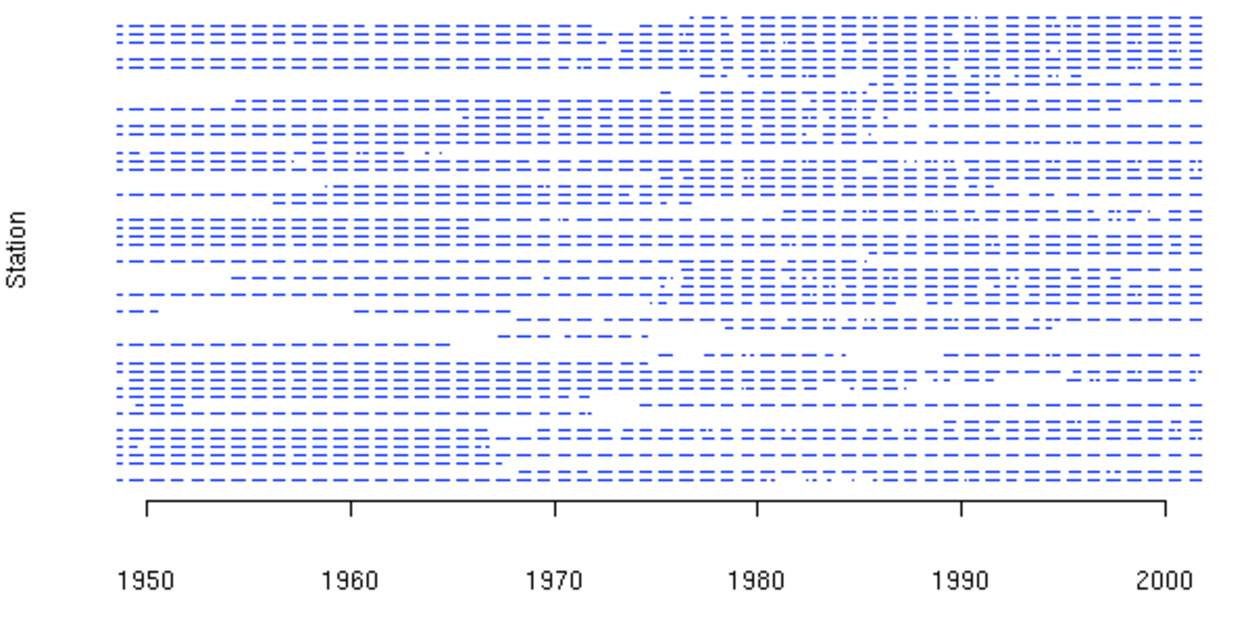
\includegraphics[width=5.5in]{Introduction/images/rainImg/operatingStations.pdf}
 \caption{Each row in this strip chart correspond to one of the 56
   weather stations in the Colorado Front Range. Blue indicates the
   days when the station was in operation, and white represents the
   days when it was not in from 1948 to 2002.  We see that some
   stations have been regularly recording rainfall since 1948, others
   have only been in operation since the mid 1970s, and still others
   have been in and out of operation over this fifty-year period.  The
   regularly spaced vertical white stripes correspond to the winter
   months when rainfall is not recorded.}
\label{fig:rainMissing}
\end{figure}
\end{center}


In addition to the precipitation values for each day, the NCAR
scientists use other information about the weather stations in their
work such as the location of the weather station, i.e.\ latitude,
longitude and elevation.

With these data, scientists examine the distribution of large
precipitation events and how this distribution may vary over
geographic location.  These are first steps toward answering important
questions such as how to assess the ability of computer climate models
to predict rainfall when they have to extrapolate irregularly located
station observations and many missing observations.  To address these
questions, statisticians use modern statistical mapping techniques and
surface fitting techniques, such as thin plate splines, in their
analyses of the rainfall data.

\subsection{Spam: Free-formatted text as data}
Well over half of the electronic email messages moving through the
Internet are ``spam'', unsolicited bulk electronic mailings.  These
unwanted messages are often offensive to read and it can be time
consuming and aggravating to sort through your inbox to delete them.
To reduce the amount of unwanted electronic mail in your inbox,
Internet providers deploy automatic spam filters (software) to
separate spam from regular email communications before it reaches a
client's inbox.  These filters need to determine whether or not an
email message is spam according to various characteristics of the
message.  Statisticians and computer scientists have had some success
with this prediction problem by using modern statistical techniques
such as Naive Bayes estimation and artificial neural networks.  For
example, Spam Assassin, a company which has developed a filter which
they describe as an
\begin{quote}
  intelligent email filter which uses a diverse range of tests to
  identify unsolicited bulk email, more commonly known as Spam.  These
  tests are applied to email headers and content to classify email
  using advanced statistical methods \textit{including a Bayesian
    statistical learning component}...
\end{quote}
Spam Assassin's email filter took top honors in 2005 in the Anti-Spam
category of Datamation's Product of the Year for their email filter,


\begin{figure}
{\footnotesize
\begin{verbatim}
Return-Path: whisper@oz.net
Delivery-Date: Fri Sep  6 20:53:36 2002
From: whisper@oz.net (David LeBlanc)
Date: Fri, 6 Sep 2002 12:53:36 -0700
Subject: [Spambayes] Deployment
In-Reply-To: <LNBBLJKPBEHFEDALKOLCIEJABCAB.tim.one@comcast.net>
Message-ID: <GCEDKONBLEFPPADDJCOECEHJENAA.whisper@oz.net>

You missed the part that said that spam is kept in the "eThunk" and was
viewable by a simple viewer for final disposition?

Of course, with Outbloat, you could fire up PythonWin and stuff the spam
into the Junk Email folder... but then you loose the ability to retrain on
the user classified ham/spam.

David LeBlanc
Seattle, WA USA

> -----Original Message-----
> From: spambayes-bounces+whisper=oz.net@python.org
> [mailto:spambayes-bounces+whisper=oz.net@python.org]On Behalf Of Tim
> Peters
> Sent: Friday, September 06, 2002 12:24
> To: spambayes@python.org
> Subject: RE: [Spambayes] Deployment
>
> [Guido]
> > ...
> > - A program that acts both as a pop client and a pop server.  You
> >   configure it by telling it about your real pop servers.  You then
> >   point your mail reader to the pop server at localhost.  When it
> >   receives a connection, it connects to the remote pop servers, reads
> >   your mail, and gives you only the non-spam.
>
> FYI, I'll never trust such a scheme:  I have no tolerance for false
> positives, and indeed do nothing to try to block spam on any of my email
> accounts now for that reason.  Deliver all suspected spam to a Spam folder
> instead and I'd love it.
> _______________________________________________
\end{verbatim}
}
\caption{An example of an e-mail message from the set of approximately
  9,000 classified messages provided by Spam Assassin for testing new
  statistical techniques and algorithms for filtering email. This
  particular mail message is not Spam.}
\label{fig:sampleEmail}
\end{figure}


To develop filtering algorithms, test cases are needed where the
electronic mail messages have been manually classified as spam or ham
(regular mail).  The collection of mail messages is used to see how
well a filter does at identifying spam as spam and ham as ham.
Spam Assassin\\
\texttt{http://spamassassin.apache.org/} has classified and made
publicly available over 9,000 mail messages, of which about 2,500 are
spam.  One of these messages appears in Figure~\ref{fig:sampleEmail}.
Spam Assassin provides each mail message in a plain text file that
includes the header, body and any attachments in the email. These
emails are organized into separate directories for spam and ham
messages.  Although these messages do not conform to our typical sense
of scientific data, they make the basis for test data required to
validate the performance of filtering algorithms.

To develop and test models and rules for predicting spam, we convert
these text messages into a format that would facilitate in-depth
statistical analysis.  For example, we might examine the body of a
mail message and record how many occurrences of various words (or even
all possible words) appear in the message.  Additionally, we might
derive variables that measure certain characteristics of the message,
such as the use of exclamation marks in the subject line, capitals in
the body of the message, and the time of day the message was sent or
received.  The task of determining which variables to create also
requires statistical investigation.  Modern statistical classification
methods have proven quite successful in all of these endeavors.

\subsection{Search and rescue: Satellite images}
On the morning of January 28, 2007, Jim Gray set sail, heading out San
Francisco's Golden Gate to the Farallon Islands, a wildlife refuge 27
miles offshore. Gray was last seen that afternoon a mile or two from
the Farallons by a naturalist who was on one of the islands, then he
disappeared.

In an article written by Steve Silberman about Gray's disappearance,
Silberman describes Gray as a ``computing legend'' whose
\begin{quote}
  work helped make possible such mainstays of modern life as cash
  machines, ecommerce, online ticketing, and deep databases like
  Google.  ``Jim's work inspired us and many other computer scientists
  to seek out and tackle very ambitious projects,'' says Google
  cofounder Sergey Brin. ``He never shied away from problems involving
  large-scale data and computation.''
  ...\\
  The notion of searching for Gray with tools he helped invent struck
  a deep chord in the online world.
\end{quote}

Friends and collaborators of Gray's got to work searching for signs of
his boat, called the Tenacious, in satellite images taken a few days
after his disappearance.  The Canadian Space Agency flew the
Radarsat-1 satellite over the area taking pictures with radar.  Then
Digital Globe's QuickBird and GeoEye's Ikonos satellites made several
passes over the San Francisco Coastline.  NASA had one of its ER-2
planes fly about 20 kilometers above the ocean taking pictures with
its near-infrared camera.  All together hundreds of gigabytes of image
data were collected.

For example, each image from the ER-2 was $4072 \times 4072$
pixels. Collaborators of Gray's at Johns Hopkins used the computer to
break up these images into smaller tiles and look for the Tenacious,
which would only be a few pixels large.  They used statistical
techniques to search the images for clusters of a few pixels with high
intensities, possibly denoting the white boat, but not too many
clusters, as that probably denoted clouds. Likely images were then
reviewed by eye to confirm whether there was something in the image
that could potentially be a sailboat.  Figure~\ref{fig:tenacious}
shows one of the tiles found through this computer vision approach.

\begin{figure}
 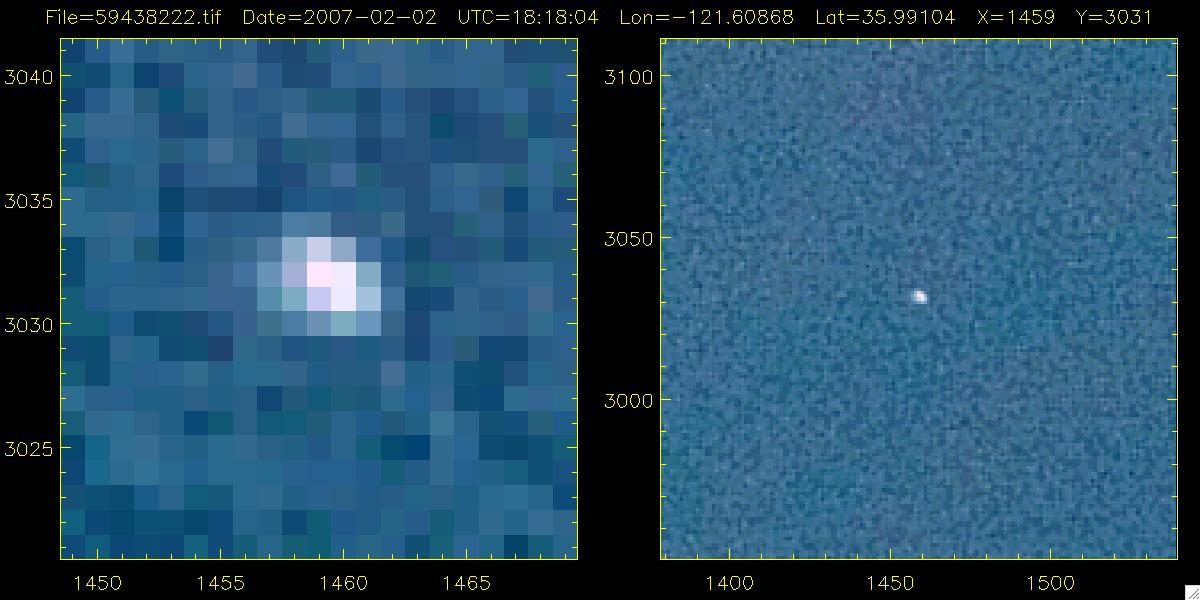
\includegraphics[width=6in]{Introduction/images/tenacious/ER-2.jpg}
  \caption{ (\url{http://skydev.pha.jhu.edu/nieto/Tenacious/images/ER-2/})}
\label{fig:tenacious}
\end{figure}

The search was particularly difficult due to the cloud cover, white
caps, wakes, and other whitish blotches on the mostly gray images.
Given the difficulty of finding ``interesting objects'' using the
computer's ``eyes'', a second effort was mounted by another
collaborator of Gray's to search through the images.  This effort, led
by a scientist at Amazon, used human eyes, or ``artificial artificial
intelligence''.  Amazon's service, called Mechanical Turk, organized
thousands of volunteers to sift through hundreds of thousands of
images looking for any sign of the Tenacious.

The Coast Guard pledged to follow any lead that any group turned up.
Several images looked promising, and ocean modelers at NASA's Jet
Propulsion Lab (also associates of Gray's) used data from Coast Guard
buoys to predict where the boat might have drifted from the time that
the pictures were taken.  Unfortunately, despite these amazing
efforts, the Tenacious was not found. Although the search failed, it
is widely recognized that these new data analysis tools that use
remote sensing images for search and rescue efforts have great
potential.


\begin{comment}
\subsection{Traffic: Video}

\begin{figure}
  \begin{tabular}{cc}
 \includegraphics[angle=90,width=3in]{Introduction/images/trafficImg/aViewfromCamera6.png}
&
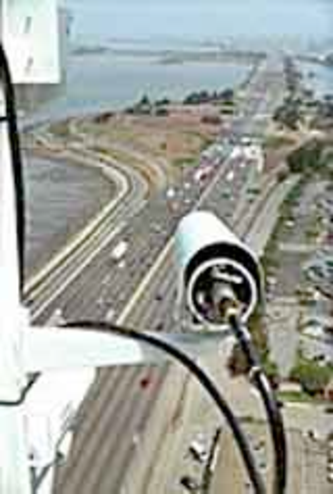
\includegraphics{Introduction/images/trafficImg/videoCam.pdf}
  \end{tabular}
  \caption{The Berkeley Highway Laboratory is a 2.7 mile section of
    Interstate 80 that's observable with a bank of twelve video
    cameras on the roof of Pacific Park Plaza, a 30-story building
    beside the freeway. The video frame from the camera shown here is
    looking north; the field of view is furthest down the freeway.  It
    covers the longest stretch (about one mile) from the Ashby Avenue
    on-ramp to University Avenue
    off-ramp. (\texttt{http://www.stat.berkeley.edu/users/fspe/I80/movie2-new.mpg})}
\label{fig:videoCam}
\end{figure}

\begin{figure}
  \begin{center}
   \leavevmode
 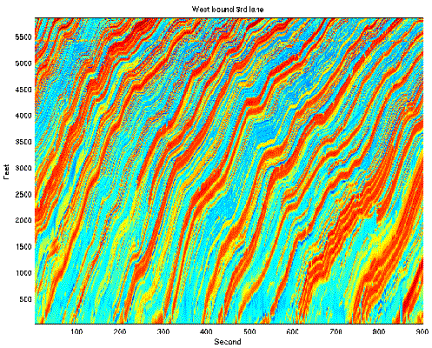
\includegraphics[width=5.5in]{Introduction/images/trafficImg/westboundLane3.png}     
\caption{A multi-colored intensity profile for a short section of 
Interstate 80 over a 15 minute time period.  (Rice and Cho \texttt{http://www.stat.berkeley.edu/users/fspe/I80/I80.htm})}
\label{fig:intensityProfile}
  \end{center}
\end{figure}


Some one about to travel on the California freeway system typically
wants to know how long it will take to arrive at their destination
and which alternate routes would be the fastest.
Transportation engineers and statisticians use a network of 
$22,000$ loop detectors located throughout the freeway system to
monitor traffic and develop such predictions. 
These detectors are embedded in the road surface and 
provide information such as the number of cars crossing over the
detector every 30 seconds, which amounts to 2GB of information 
collected a day.  
Using past traffic patterns and current condition as supplied by these 
detectors, statisticians fit models to predict the fastest route
from one location to another.


To improve the quality of the predictions, scientists are now exploring
the use of video cameras to complement existing loop detectors. 
The Berkeley Highway Laboratory has mounted video cameras on top of buildings
near a section of Interstate 80 to monitor traffic on the freeway
(see Figure~\ref{fig:videoCam}).

These video data have the advantage over loop detectors in that they
are easy to maintain and they provide better spatial coverage.
However, they present real challenges related to computer vision,
i.e.\ how can computers ``see'' the cars on the freeway in the video
recordings?  Statisticians have developed techniques based on the
behavior of stochastic processes to convert these low-resolution
images into information about traffic intensity across time and space.
For example, the multi-colored intensity profile in
Figure~\ref{fig:intensityProfile} describes the aggregate behavior of
vehicles in a stretch of the middle lane of the westbound traffic over
a brief fifteen minute time period. With this information in hand,
algorithms can be developed and tested that pull out useful
information such as the speed of traffic at a particular location.
\end{comment}

\section{The  Data Analysis Process}
None of the data in the examples of  the previous section come in
a traditional row-column format that is ready for statistical
analysis.  The missing recordings of rainfall need to be carefully
investigated before proceeding with a more in-depth analysis of the
distribution of extreme weather events.  The email messages require a
lot of processing in order to extract useful information for
developing a prediction procedure, and the cloud cover and temporal
nature of the images needs to be considered when searching
for small, high-intensity clusters.  Most
statistics texts limit their exposition of data analysis to examples
where data have already been distilled into a rectangular table of
numbers that are prepared for the application of a particular
statistical method.  To use common statistical methods, we may end up
projecting the raw data into a rectangular array of numeric values.
However, the process of figuring out how to create these variables
from raw input is an important part of the data analysis process.  Our
goal here is to bring to the forefront this entire process, which
includes the need to be able to acquire, clean, and summarize data,
as well as to model and validate the model with data, and to 
report findings from the analysis.

Handling raw data is both interesting and non-trivial.  It requires a
facility with data analysis and also the ability to express
computations that help readily explore the many different ways to
reduce the information into a format for further, deeper analysis.
Curtailing the data analysis process in this way can greatly impact a
statistician's ability to do interesting, high-qualilty analysis.
That is, not being able to work directly with the raw data limits a
scientist greatly.  Analyzing data requires knowledge about the
particular topic being studied and of appropriate statistical methods,
and it also requires the ability to be able to apply those methods to
the relevant data.  This includes accessing the data values,
transforming them into the appropriate form, applying statistical
methods to the data and exploring the results.  Computing and data
technologies are as essential for data analysis as understanding what
statistical methods are appropriate for the data.  Computation is the
vehicle by which we move data into information.

One must be able to access data in different forms, examine them to
see what one has, find relevant subsets, model them or find the
``signal'' and iterate these steps and ultimately report ones
findings.  This iterative cycle of data analysis requires facility
with one or more computer languages so that expressing the
computations fades into the background and becomes a means to an
end. It should not be a hurdle that diverts one from the data analysis
task and scientific question.  For this to be true, one must take
learning computing seriously and try to understand it rather than
simply parrot examples. A good understanding of these fundamental
ideas and concepts will be of immense value to you in whatever field
you pursue as it will surely involve decision making, data and
computation.


Even when our focus is not on a particular scientific problem or set
of data, but rather in understanding characteristics of mathematical
or statistical methodology itself, the computer is a terrific new tool
at our disposal.  In the past, we relied almost exclusively on
mathematical techniques to explore a particular method and how it
would behave under different circumstances.  When doing research, we
might have attempted to prove a mathematical result without really
knowing if it were true or not.  We can now use the computer to
simulate the behavior of a method to gain a better understanding and
to gain intuition about its behavior.  With intelligent experimental
design, we can vary the inputs to a simulation to more efficiently
understand the different characteristics of a computational approach.
And the computer therefore serves as an additional tool along with the
more traditional mathematical approach.  And these two serve as
complementary media for describing and discussing scientific research.



\begin{comment}
\section{Overview of material covered}

As we mentioned above, we will discuss the different stages in the
data analysis cycle from start to end.  We won't emphasize the
statistical methodology, but we will introduce both general
computational techniques such as the bootstrap and cross
validation. Also, we will make use of methodology that you may not
have seen in other statistics classes and we will provide a brief,
heuristic introduction to each of these.

We focus on scientific questions and how we might acquire, summarize,
clean, model and report the data and results.  This is not about
applying statistical methods to example data. Rather the question
tells us what statistical techniques might be relevant and
appropriate. Some of these are complex and some are simple. We prefer
the simple approach if it is adequate and in keeping with the
scientific question and the accuracy and precision needed in the
answer.  Please don't use statistical techniques that are not
appropriate or overkill for the task at hand. Start by looking at the
data and producing interesting, meaningful graphical summaries.  Well
composed (the thinking process) and created (via software) plots are
often the most compelling answers.  Blind use of linear models tend to
be superficial and associated with a mechanized response rather than
an understanding of the particular data.

These examples all have a similar structure when it comes to answering
a question with data --

     \begin{itemize}
     \item Data ACQUISITION --- Input/output, regular expressions 
     \item Data CLEANING, verification, and manipulation --- graphics, exploratory data analysis
     \item Data ORGANIZATION --- data frames, XML, databases
     \item MODEL the data --- fit statistical models to the data 
     \item Data as a PSEUDO-POPULATION --- assess the fit of the model via the
     bootstrap, cross-validation 
     \item SIMULATED data --- simulation studies 
     \end{itemize}

In this cycle we encounter: 
\begin{itemize}
\item Statistical Concepts
\item Computing Concepts
\item Software
\end{itemize}

These three concepts will be interwoven throughout 
the text. 

In the book, we will look at various data and computing technologies.
These include
\begin{itemize}
\item the R statistical computing language and environment;
\item simulation and random number generation;
\item bootstrapping for estimation, and cross valdation for model selection;
\item processing text with pattern matching via regular expressions;
\item simple data manipulation and analysis using shell tools;
\item parsing structured data in the form of XML --- the eXtensible Markup Language;
\item accessing remote, structured data in relational database
  management systems via the client-server model of computing
and SQL --- the Structured Query Language.
\end{itemize}
This involves at least five different languages.
We could explore other languages such as Perl
and Python, but we won't as we can do most things using
R and the shell tools.  But one should be aware of these
other languages and tools.

We will also cover aspects of visualization, both the basic aspects of
using R to produce plots and also how to think about what plots to
create.  And we will encounter some non-classical, even modern,
statistical methods such as classification and regression trees, k-th
nearest neighbor classification, Bayesian models, thin plate splines
(TSP).



\subsection{Statistical Concepts}

\begin{itemize}
\item Graphics
        \begin{itemize}
        \item elements of graphing data
        \item grammar of graphics
        \item advanced plotting
        \end{itemize}

\item Computationally intensive methods
        \begin{itemize}
        \item Classification and Regression Trees
        \item Kth Nearest Neighbor clustering
        \item Thin plate splines 
        \end{itemize}

\item Simulation tools 
        \begin{itemize}
        \item Bootstrap
        \item Cross-validation
        \item Monte Carlo Markov Chain 
        \end{itemize}
\end{itemize}

\subsection{Computing Concepts}

\begin{itemize}
\item Programming concepts - e.g. loops, recursion, trees

\item Regular expressions and text manipulation

\item Relational Databases

\item Random number generation

% \item Representation of numbers in the computer 

% \item Event handling and GUI development
\end{itemize}

\subsection{Software}

\begin{itemize}
\item R - statistical software
\item Unix - shell commands
\item Regular expressions
% \item Perl 
\item SQL - Structured Query Language for relational databases 
\item XML - Extensible Markup language
% \item Gtk - GNU Toolkit for creating graphical user interfaces
\end{itemize}

\end{comment}

\begin{comment}
\section{Goals of the Course}
\begin{itemize}
\item
  Focus:  use existing software and functionality
   for context-specific analyses.
\item
  Learn about: box of tools and how to use them
   to create things, and even build new tools.
   \\
   Learn about currently emerging technologies
\item
   De-emphasize: understanding the existing algorithms.
  \\
     Be able to intelligently discuss different 
     technologies and tools, knowing when to use them and what are
     the trade-offs

\item
    Understanding fundamental algorithms is important 
    if you need to
\begin{itemize}
\item
    recreate them in a new language
\item
    use them in new ways when developing new algorithms.
\end{itemize}

\item Practical: how statistical methodology is used
    in Industry, Laboratory, Research 

\item
  Focus: overall task not just on the application of 
  specific statistical methodology but on 
  how to think about approaching problems related to
  computing on data
\end{itemize}

 

\begin{itemize}
\item
  How to think about approaching problems related to
          computing on data
\item
  Learn about currently emerging technologies
\item
  Be able to intelligently discuss different 
     technologies and tools, knowing when to use them and what are
     the trade-offs
\item
  Be able to find out about and learn other technologies
\end{itemize}
\end{comment}


\setcounter{chapter}{1}
\chapter{Computing with Digital Information}
It is common knowledge that personal computers have become faster at
an incredible rate since they were first introduced in the mid-1970s.
But how fast are they, and how fast were they even five years ago?  A
quick Internet search leads us to the ``How Stuff Works'' Web page at
microprocessors\\
{\footnotesize{\texttt{http://computer.howstuffworks.com/microprocessor1.htm}}}\\
where we find the table shown in Figure~\ref{fig:HowStuffWorks}.  Run
your eyes down the columns of numbers and it's clear that the chips
have grown tremendously in terms of numbers of transistors, clock
speed, and MIPS.  But, it's difficult to see the rate of change,
e.g. Has the growth been exponential? Have these various measures
grown at the same rate?


\begin{figure}
\begin{center}
\begin{tabular}{c}
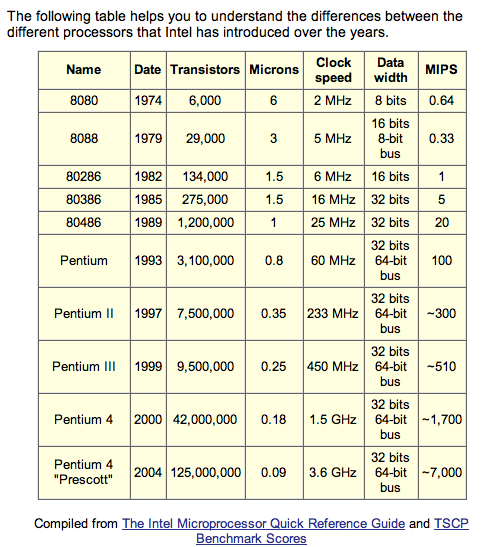
\includegraphics[width=5in]{computerIntro/images/howStuffWorks.png}
\end{tabular}
\caption{This screenshot taken from the ``How Stuff Works'' Web page
  {\footnotesize{\texttt{http://computer.howstuffworks.com/microprocessor1.htm}}}
  compares the various Intel chips since the 8080 chip was first
  introduced in 1974.  The Intel microprocessor has become much
  faster, smaller, and more powerful in the past thirty years, as seen
  by several measures.  From left to right, these measures are the
  number of transistors on the chip, the width in microns of the
  smallest wire on the chip, the clock speed (number of cycles per
  second), the number of bits used for addressing data in RAM, and the
  number of instructions processed per second (in millions).  The plot
  in Figure~\ref{fig:chip} shows a comparative picture of the changes
  in these variables over time.}
\label{fig:HowStuffWorks}
\end{center}
\end{figure}


To answer these questions, we need to get the data out of the Web page
in order to plot or compute rates of change from these measurements.
To extract the data, we could copy and paste from the browser into an
Excel spreadsheet or a plain text file, and then edit a bit to fix up
any errors made in the copy and paste.  Or, we could simply type the
numbers into Excel or a plain text file.  Table~\ref{tab:chip} and
Figure~\ref{fig:csvExcel} show the data in these new formats.  Neither
of these approaches are necessarily recommended because they are prone
to error, do not leave a trail of the process used to create the data,
and can be cumbersome if the process needs to be repeated in the
future (e.g. when a new processor is introduced).  Later chapters will
provide alternative ways to get data out of a table on the Web page
and into a format more conducive to further analysis.

\begin{table}
{\footnotesize{
\begin{verbatim}
Name       Date  Transistors Microns  Speed Units Data 	MIPS
8080       1974       6000     6        2   MHz    8       0.64
8088       1979      29000     3        5   MHz   16       0.33
80286      1982     134000     1.5      6   MHz   16       1
80386      1985     275000     1.5     16   MHz   32       5
80486      1989    1200000     1       25   MHz   32      20 
Pentium    1993    3100000     0.8     60   MHz   32     100
PentiumII  1997    7500000     0.35   233   MHz   32     300
PentiumIII 1999    9500000     0.25   450   MHz   32     510
Pentium4   2000   42000000     0.18     1.5 GHz   32    1700 
Pentium4x  2004  125000000     0.09     3.6 GHz   32    7000
\end{verbatim}
}}
  \caption{An alternative format for the data in Figure~\ref{fig:HowStuffWorks}: a plain text table, where the measurements are separated by blank spaces.}\label{tab:chip}
\end{table}

\begin{figure}
\begin{center}
\begin{tabular}{c}
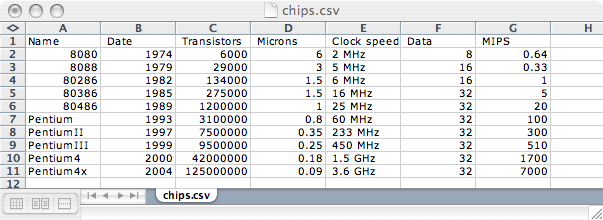
\includegraphics[width=5in]{computerIntro/images/excelScreenshot.png}
\end{tabular}
\caption{A screen shot of an alternative format for the data in
  Figure~\ref{fig:HowStuffWorks}: an Excel spreadsheet of the data.}
\label{fig:csvExcel}
\end{center}
\end{figure}

With the plain text file, we can easily read the data into the
statistical software R, and examine graphically the changes in the
number of transistors, the width of the smallest wire, the clock
speed, etc. of the Intel chip.  Figure~\ref{fig:chip} shows how the
Intel chip has experienced exponential growth according to all of
these measures, with the change in the width of the smallest wire
having the slowest growth (Note that it is the rate at which the
thickness has decreased which is plotted for this variable).  In a
way, it is not all that surprising that the other three measures are
very similar because clock speed and MIPS are directly related to the
number of transistors on the chip.

\begin{comment}
The code for preparing the data to make the plot appears below.  In
later chapters, we will cover the R statistical software in greater
detail, but for now notice that the five lines of code do the
following tasks: read in the data from a plain-text file; change the
values in Speed so that they all have the same units, i.e. MHz; select
the variables to be examined; normalize these variables by the value
in the initial year so the measurements become relative to 1974; and,
finally, invert the Microns measurement so it is increasing rather
than decreasing. Once the data have been transformed, they can be
plotted as in Figure~\ref{fig:chip}.
{\footnotesize{
\begin{verbatim}
chips = read.table("Chip.txt", header = TRUE, row.names = 1)
chips$Speed[ chips$Units == "GHz" ] = 
     1000* chips$Speed[chips$Units =="GHz"]
measures = c("Transistors", "Speed", "Microns", "MIPS")
chipsRate =  chips[measures]/as.numeric(chips[1, measures])
chipsRate$Microns = 1/chipsRate$Microns
\end{verbatim}
}}
\begin{verbatim}
matplot(chips$Date, chipsRate, 
  type="l",  log="y", lwd=2, lty=1, 
   ylab= "Growth in comparison to 1975 - log scale",
   xlab= "Date", col= c("black","red","green","blue"))

varl = names(chipsRate)
legend(1976, 1000, legend=varl, fill=coll, bty="n")

 abline(v=1993, col="grey")
  mtext(text="Pentium", side=3, line=-1.2, at=1993+0.1,adj=0)
 abline(v=1985, col="grey")
 mtext(text="32 bit processor", side=3, line=-1.2,at=1985+0.1,adj=0)
\end{verbatim}
\end{comment}

\begin{figure}
\begin{center}
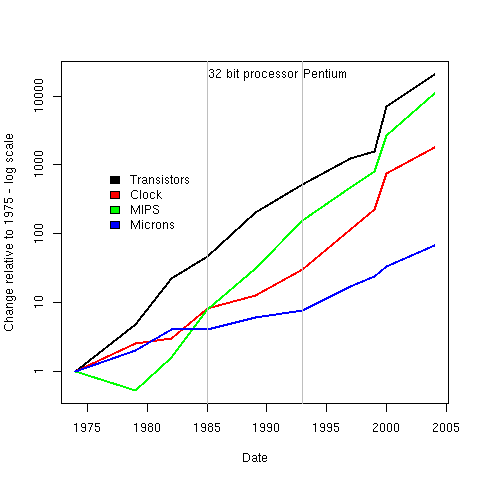
\includegraphics[height=4in]{computerIntro/images/bestChips.png}
\caption{This graphical display of the data from the plain-text table
  of values in Table~\ref{tab:chip} shows how the computational
  power of the Intel microprocessor has grown exponentially over the
  past thirty years. The grey lines mark the introduction of the
  32-bit processor and the Pentium processor in 1985 and 1993,
  respectively.}
\label{fig:chip}
\end{center}
\end{figure}

By now, you may be wondering: What is a microprocessor and what are
MIPS and Clock speed?  What is the difference between a table in a Web
page, an Excel spreadsheet, and a plain-text table?  What are these
computation in R doing?  These questions are important to
understanding basic notions in data technology.  One doesn't need to
be a techno-wizard to use a computer to analysze data, but there are
some fundamental concepts that can make a big difference in helping
you take full advantage of the tools available for handling data.
Addressing these questions are the topic of this chapter.

In Section~\ref{sec:computation} we introduce some terminology that we
use to describe computations and the basic syntax for carrying out
statistical computations in R.  This section leads into a brief
overview of the various types of computing languages, e.g. compiled
and interpreted languages, and examples of them
(Section~\ref{sec:languages}).  Next we examine how information, such
as text, numbers, and images are represented in a computer and how
they are organized into files and directories
(Section~\ref{sec:digital}).  The chapter concludes with a brief
description of basic the components of a computer
(Section~\ref{sec:components}). If you are already quite familiar with
these topics then you may want to skim this chapter.


\section{Computations}\label{sec:computation}
The instruction set on a computer chip provides the basic primitives
with which we can build more sophisticated, higher-level computations
to, for example, add a vector of numbers, sort a list of names, and
make a plot.  Whether primitive, complex, or high-level, a computation
acts on one or more inputs to create an output, and it can be thought
of as a transition from an old state to a new state: to add a set of
numbers, we take the various numbers as inputs and create one output
-- the sum; to sort a list of names, the input list of names
transitions to an alphabetically sorted list; and to make a plot of
the change in microprocessors in the past thirty years, the computer
acts on the data (Table~\ref{tab:chip}) to produce the image shown
in Figure~\ref{fig:chip}.

In general, we \Key{invoke} a computation with an
\Key{expression}. For example, the expression \RCode{17 + 100} is
handed off to the computer for \Key{evaluation}; the inputs, $17$ and
$100$, are acted on, and the \Key{return} value of the expression is
$117$.  The plus sign \RCode{+} is an \Key{infix operator}, meaning
that it comes between its inputs ($17$ and $100$).  The R language
uses both infix operators such as $+$, $*$, \verb+^+, $/$ for
addition, multiplication, exponentiation and division, respectively,
and it uses \Key{function style computations}.  Function style
computations in R have the general format,
\begin{verbatim}
functionName(argument, ... , argument)
\end{verbatim}
For example, \RCode{rnorm(3)} invokes the \RCode{rnorm} computation to
generate three random normal values. That is, the input to the
function \RCode{rnorm} is $3$, and the output is $3$ numeric values
that are randomly generated from the normal distribution.
\begin{verbatim}
-2.2994024 -0.4127883  0.1197349
\end{verbatim}

The arguments in a function-style computation can also be identified by
name.  The computation below provides the inputs $3$, $2$ and $1$ to
the computation in order to generate $3$ random values from a normal
distribution with mean $2$ and standard deviation $1$.
\begin{verbatim}
rnorm(3, mean = 2, sd = 1)
2.8913993 -0.4770861  2.7620108
\end{verbatim}
The details of the syntax for the R language are covered in greater
detail in Chapter~\ref{chap:RIntro}.

The \Key{single expression} \RCode{rnorm(3, mean = 2, sd = 1)} can be
nested within another expression to create a \Key{compound expression}
such as
\begin{verbatim}
mean(rnorm(3, mean = 2, sd = 1))
\end{verbatim}
which returns $0.7153243$, the mean of three random normal values
(notice that we get a new set of three random normals when we invoke
the \RCode{rnorm} computation again).  Here the output from the \RCode{rnorm}
expression becomes the input to the \RCode{mean} function.

If an expression is \Key{ill-formed} then the output will typically be
an error message.  The output from the computation,
\begin{verbatim}
mean(rnorm(3, mean = 2; sd = 1))
\end{verbatim} 
is the text message
\begin{verbatim}
Error: syntax error in "mean(rnorm(3, mean = 2;"
\end{verbatim}
Rather than returning the mean of three random normal values, the
output of the computation indicates we have not properly written the
expression.  Computing languages are not very forgiving when we make simple
typing errors.  Although most people would understand that the
semicolon and the comma in the expression most likely mean the same
thing, the computer language does not make such guesses or
assumptions.  It has very specific rules for breaking down an
expression into parts to determine what to do.  This \Key{parsing} of
the expression into \Key{tokens} is based on particular syntax
rules. To separate out the pieces of an expression, R uses a variety
of techniques.

\begin{itemize}
\item An \Key{atomic token}, such as \verb-+-, separates the
                                            expression $2+3$ into the
                                            three tokens, $2$, $+$,
                                            and $3$.
\item \Key{White space} or blank spaces between digits and characters
  split an expression into sub-pieces.  If blanks are added to the
  above expression, e.g. $2~~+~~3$, the expression is divided into the
  same three tokens.  In this example, the white space helps us read
  code more easily, and the R language does not care whether there are
  extra blanks between the tokens.
\item \Key{Parentheses} determine the order of execution in an
  expression, e.g. $(2+3)*6$ is $30$, not $20$. They are also used to
  mark the inputs to a function-style expression as in
  \RCode{rnorm(3)}.
\item \Key{Commas} separate the inputs to a function-style expression,
  e.g.  \RCode{rnorm(3, 1)}.
\item A \Key{new line} typically separates expressions.  However, more
  than one expression can appear on one line, provided the expressions
  are separated by \Key{semicolons}. The two expressions below are
  evaluated and both of their outputs returned.
\begin{verbatim}
rnorm(3) ; 17 + 100
 -0.7120203 -0.1849239  1.4615504
 117
\end{verbatim}
\item \Key{Naming conventions} also aid in parsing.  Names must begin
  with a letter or a period and may contain upper and lower case
  letters, numbers, and a few special characters such as the period
  and underscore.  So \RCode{2*rnorm} cannot be a name, but instead
  must be the expression \RCode{2 * rnorm}.
\item \Key{Quotation marks} distinguish character values from names of
  functions and variables.  The style of beginning and ending quotation marks
  must match.  For example, \verb+"Hi"+ and \verb+'Bye'+ are valid
  character values, but \verb+"My'+ is not.
\end{itemize}

When we evaluate an expression in R, the result prints to the screen
as output.  If we want to use the result in another expression, we can
form a compound expression.  However, if we need to use the result in
more than one subsequent expression, then we must \Key{assign} the
output from an expression to a \Key{variable}. The statement 
\begin{verbatim}
 x = rnorm(4)
\end{verbatim} 
assigns the four numeric values from the \RCode{rnorm} computation to the variable
called \SVariable{x}.  Note that the equal sign takes a very special
meaning in R, and in many other programming languages as well.  The
variable named on the left-hand side of the equal sign is assigned the
output value returned from the expression on the right-hand side of
the equal sign. So, $=$ is an infix operator itself that assigns the
input on the right-hand side to a location with name provided on the
left-hand side of the operator.

Variables have a \Key{name} and a \Key{value}.  To access the value we
use the name.  That is, we can see the value of $x$ via the simple
expression
\begin{verbatim}
x
\end{verbatim}
It returns
\begin{verbatim}
0.04850939 -1.25439102  0.68716756 -2.35116688
\end{verbatim}
the four random normal values.  The simple expression \RCode{x}, is a
computation that is the equivalent of: evaluate x and print the
result.  In other words, provide the current contents of the variable
\SVariable{x}.

Variables allow us to:
\begin{itemize}
\item store state on the computer
\item store a value without needing to recompute it
\item write a general expression, e.g. sqrt(a\^~2 + b\^~2)
\item reduce redundancy (and mistakes)
\end{itemize}
For example, in the R code below, the variable \SVariable{n} is
assigned the value $10$, then \SVariable{n} is used twice: once to
specify the number of random normal values to generate and a second
time as the divisor in the mean computation.
\begin{verbatim}
n = 10
x = rnorm(n)
sum(x) / n
\end{verbatim}
Of course, we could have used the value $10$ in the \RCode{rnorm} and
\RCode{sum} expressions, but then if we want to change the computation
to instead generate $100$ random normals and take the average, then we
need to change the $10$ to $100$ in two places.
\begin{verbatim}
x = rnorm(100)
sum(x) / 100
\end{verbatim}
Although this is a simple example, we can imagine how it would be easy
to make a mistake and only change one of the two $10$s to $100$, which
would lead to an incorrect answer which may even go undetected.

A few words of advice on variable names: they must follow the naming
conventions described earlier, and in addition, it is helpful to use
meaningful names because it makes it easier to understand code.  Also,
it is best to avoid names that have a special meaning in R because
they can be confusing when reading code and they can lead to
unexpected undetected errors if there is an error in your code.  For
example, the function names such as \RCode{c}, \RCode{t}, \RCode{s}
are best avoided.

\subsection{Example: Generating Pseudo-random Numbers}
An \Key{algorithm} is a set of directions for carrying out a computation in
terms of other simpler computations. One example is the algorithm that
a computer uses to generate random numbers.  In fact, most computers
do not generate truly random numbers.  Rather, they generate numbers
that ``look'' random, using numerical algorithms.  These pseudo-random
numbers are in fact deterministic; when you start the algorithm at a
particular initial value, then the random-number generator produces
the same deterministic sequence of numbers.  However, the numbers
produced look very much like random numbers, and this determinism can
be very useful when we want to be able to reproduce our ``random''
results at a later time.


\begin{comment}
  For example, consider the two coin tossing sequences in
  Figure~\ref{fig:coinflip} produced by an eighth grade class.  One
  half of the class flipped a coin $100$ times and recorded a $1$ or
  $0$ according to how the coin landed.  The other half of the class
  concocted a pseudo-random sample.  Many people incorrectly identify
  these two sequences.  This very simple probability distribution
  where $0$ and $1$ each occur with chance $1/2$ and where one toss
  does not depend on the next, can produce random sequences that do
  not look random to the casual observer because there are often
  longer than expected runs of $0$s or $1$s.  If we count the number
  of switches from one to zero and zero to one and the length of the
  longest run for each of the sequences in Figure~\ref{fig:coinflip}
  and compare them to what we would expect to get if the sequence
  really were random, then the fake sequence stands out.
  Surprisingly, it is the sequence with the shorter runs. It is
  important to have good, well-tested pseudo-random number generators.

\begin{figure}
   \begin{center}
   \begin{tabular}{ccc}
   00111000110010000100 & \ \ \ \ \ \ \ \ \ \ & 01000101001100010100 \\
   00100010001000000001 &                     & 11101001100011110100 \\
   00110010101100001111 &                     & 01110100011000110111 \\
   11001100010101100100 &                     & 10001001011011011100 \\
   10001000000011111001 &                     & 01100100010010000100
   \end{tabular}
   \end{center}
   \caption{Two binary sequences produced by students in an eighth
     grade class. One sequence was generated by one group of students
     flipping a coin 100 times and recording $1$ for Heads and $0$ for
     Tails.  Another group of students who were instructed to fake the
     $100$ flips.  Can you figure out which is the actual sequence of
     $100$ coin flips and which is the fake?}
\label{fig:coinflip}
\end{figure}
\end{comment}

Pseudo-random number generators are put through a battery of
statistical tests to evaluate their randomness.  
\begin{comment}The typical computer
does not have a coin flipping mechanism within it, and instead we rely
on numerical algorithms to generate fake random numbers.  
\end{comment}
One well
known algorithm is the \Key{congruential generator}.  The congruential
method uses modular arithmetic to generate ``random'' numbers.  From
inputs $a$ and $b$ and an initial value, $x_0$, the first ``random
number'' is generated as follows:
$$ x_1 = a * x_0 \mod b, $$
and subsequent numbers are generated recursively,
$$ x_{n+1} = a * x_n \mod b .$$
In R, the modulo function is represented by the infix operator
\verb+%%+, i.e. 
\begin{verbatim}
NextValue = (a * CurrentValue) %% b
\end{verbatim}

So, for example, if $a=3$, $b=64$, and our starting value, which is
called the \Key{seed}, is $17$ then the sequence of values produced by
the congruential method for these inputs appears below.

\medskip

\begin{tabular}{l|ccccccccccc}
iteration & 0 & 1 & 2 & 3 & 4 & 5 & 6 & 7 &  8 & 9 & 10 \\
\hline
value &17 & 51 & 25 & 11 & 33 & 35 & 41 & 59 & 49 & 19 & 57 \\
\\
iteration &11 & 12 & 13 & 14 & 15 & 16 \\
\hline
value & 43 & 1 &  3 & 9 & 27 & 17 \\
\end{tabular}

\medskip

Notice that by the $16^{th}$ iteration the sequence has repeated.
With proper choice of the constants $a$ and $b$, it takes longer for
the numbers to repeat and they have a more random appearance. See
Figure~\ref{fig:congPlot} for an example.

\begin{figure}
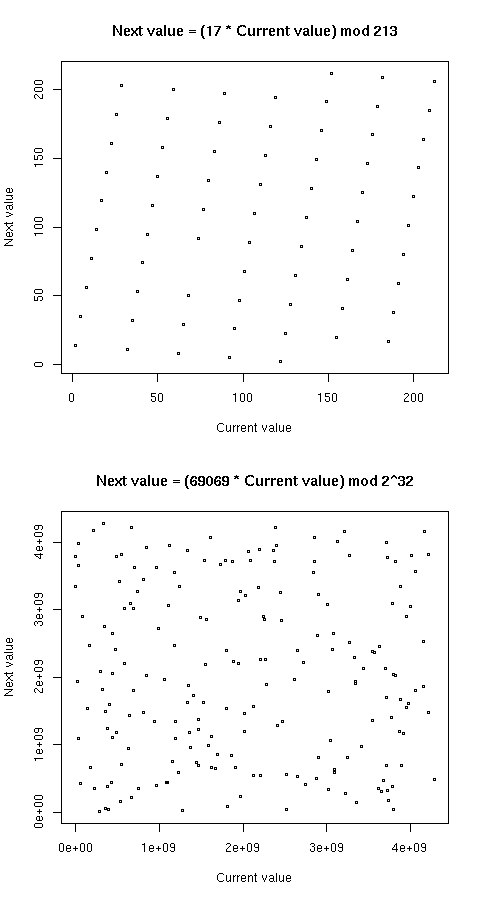
\includegraphics[height=6in]{computerIntro/images/cong.png}
\caption{For each scatter plot, two hundred values, $x_1$, $x_2$,
  \ldots, $x_{200}$ are generated according to the congruential
  method.  The points represent successive pairs of numbers,
  e.g. $(x_1, x_2)$, $(x_2, x_3)$, etc.  In the top plot, the method
  uses the algorithm $x_{n+1} = 17x_n~mod~213$, and the bottom plot
  uses the default values from one of R's generators, $69069x_n
  ~mod~2^{32}$.  The seed is $17$ in both cases. The first set of
  values show a stripy non-random pattern whereas the second set
  looks randomly scattered. }
\label{fig:congPlot}
\end{figure}


Several random number generators are offered in R. These are discussed
in Section~\ref{sec:repNum} as their designs are connected to the
representation of numbers in the computer.



\section{Understanding the R Language}\label{sec:languages}
When learning a programming language, one typically needs detailed,
specific information about particular syntactic structures such as how
to write a conditional statement or a loop or what are the inputs for
a particular function, but it is also important to have a broad ``big
picture'' understanding of the language.  Like with a human language,
one needs to become familiar with the rules of the language, but also
the vocabulary and the style and idioms that others use.  And for a
computer language, it helps and is important to understand the
rationale and logic that underlies how the language is understood by
the computer.  This helps you express computations properly and
understand why the computer may interpret the commands differently
from your expectations.

\begin{comment}
%this belongs in a different chapter
There are several sources of information about the R and S programming
languages that work at these different levels of specific information,
reference manuals and broad overviews.  In this chapter, we don't
attempt to provide all of these.  Rather, here we focus on trying to
understand the rationale of the language. We expect the reader to
explore the ideas interactively using the R environment as they read
this and do some experiments to see how the language works.  We have a
terrific, interactive medium with which we can hypothesize and test
characteristics.
\end{comment}

Finding out how R works and learning to think about how to express
computations in R will greatly simplify your work when using R. It is
good to take the time early on to learn a language and not simply use
it in a utilitarian, ad hoc manner.  And while R is a specific
language that you may or may not use extensively in the future, it is
important to realize that what you will learn when exploring R will be
generally applicable to many different programming languages that you
might use.  R is very similar to Matlab, and shares many of the same
concepts as Perl, Python, Java, C, and FORTRAN.  Although they are all
quite different, they also share important commonalities that are
essential when communicating about computations to others and to the
computer.

R is both an interactive and interpreted language.  By interpreted, we
mean that we can give an instruction and immediately have it
evaluated.  Then, we can give another command.  In other,
non-interpreted languages, we must write an entire program made up of
a sequence of commands that are specified before we run the program.
We have to order the instructions and take account of different
possibilities.  Once the program is running, we cannot change the
commands.  All we can do is either wait for it to complete or
terminate it and re-run it with the commands altered or different
inputs.


Interactivity is very important for statisticians.  We need to be able
to visualize data, look at numerical summaries and the output from
fitting a model, or subsetting the data based on previous observations
and then decide what to do next.  This process has been given the
name, Exploratory Data Analysis, or EDA for short.  It is a highly
iterative process where we attempt to let the data direct us as to
what to do next.  We try different things as we go along different
branches or paths. Sometimes these lead to useful insights that we
want to report. At other times, they verify that certain assumptions
are justified, or they suggest trying different methods to better
understand the data.  The ability to dynamically specify what we want
to do next is important.  R then allows us to combine commands into a
script or ``program'' that we can re-run on new or different data to
recreate our analyses.  This is often termed \textit{batch}
programming since we are doing several commands in a single run. This
combination of interactive commands and running scripts in a batch
gives us the best of both worlds: we use interactive facilities during
exploration, and programming facilities when the exploration is more
``complete''.


\section{Digital Information}\label{sec:digital}
A computer is a general purpose information processing machine.  The
information it can process could be a movie on DVD, a collection of
photos on a CD, a Web page on the Internet, an Excel spreadsheet
stored on a memory stick, or a plain text file on the computer's hard
drive.  All of these examples are digital because computers are
digital devices.

The smallest unit of information in a computer has just two states.
For example, CDs and DVDs are optical storage devices that use two
different levels of light reflectance to represent information.  Also,
memory cells in a computer are either charged or cleared, and magnetic
storage devices like the hard drive in a computer have areas that are
either magnetized or not.  These two states can be represented by the
binary digits 1 and 0.  Binary digits are the building blocks for all
information processing in computers.

The term ``bit'' is an abbreviation for binary digit. Interestingly,
it was a statistician from Bell Labs, John Tukey, who coined the term
in 1946. While information is made up of bits, we typically work
at the level of ``bytes'' and higher level entities.  A byte is a unit
of information built from eight bits.  The notion of a byte was first
used in encoding characters. For example, the 8 bits, $01000001$
encodes the capital letter \verb+A+.

\subsection{Characters}\label{sec:characters}
In order for digital devices (hard disks, CDs, DVDs, etc.) to process
and store text information we need a correspondence between bit
patterns and the symbols of a written language, which are called
glyphs.  ASCII (American Standard Code for Information Interchange)
was created in the early 1960s as a bit encoding for the English
alphabet. It uses seven bits to represent character glyphs.  For
example, $1000001$ represents the upper case \verb+A+, the glyph
\verb+B+ is coded as $1000010$, \verb+C+ is $1000011$ and so on.  The
eighth bit in an ASCII byte is typically set to zero, although
historically it was used for error checking.

Modern character encodings support many more characters, while also
typically remaining compatible with ASCII.  One example is Unicode.
It uses 16 bits to encode characters, rather than 7.  Unicode is an
industry standard designed to allow text and symbols from all of the
writing systems of the world to be consistently represented and
manipulated by computers.  The first 128 characters ($2^7= 128$) of
Unicode are compatible with ASCII.  See Table~\ref{tab:ASCII} for
examples of the ASCII and Unicode mapping from bits to glyphs.

\begin{table}
\begin{center}
\begin{tabular}{ccc|cc}
  \multicolumn{5}{c}{Binary Representations of Characters}  \\
Glyph & ASCII & UniCode & Glyph & Unicode \\
\hline
\# & 0010 0011 & 0000 0000 0010 0011 & \copyright & 0000 0000 1010 1001 \\
\$ & 0010 0100 & 0000 0000 0010 0100 & \ae  & 0000 0000 1110 0110 \\
A & 0100 0001 & 0000 0000 0100 0001 & $\Delta$ & 0000 0011 1001 0100\\
a & 0110 0001 & 0000 0000 0110 0001 & $\alpha$ & 0000 0011 1011 0001\\
\hline
\end{tabular}
\caption{A few examples of the mapping from glyph character to ASCII
  and Unicode.  ASCII uses 7 bits to represent characters (with the
  eighth bit typically set to 0) and Unicode uses 16. The ASCII and
  Unicode mappings are compatible for the $2^7 = 128$ ASCII
  characters.  The two glyphs on the bottom right of the table (the
  Greek letters, capital delta and lower case alpha) do not have
  encodings in ASCII. }
\label{tab:ASCII}
\end{center}
\end{table}


The table on the How Stuff Works Web page
(Figure~\ref{fig:HowStuffWorks}) and the plain text table in
Table~\ref{tab:chip} are both encoded in ASCII, while the Excel
spreadsheet (Figure~\ref{fig:csvExcel}) stores the data in a
different encoding.  Although the information is essentially the same
in all three contexts, there are important differences between them.
These are described in Section~\ref{sec:electronicFiles}.


\subsection{Representation of Numbers}\label{sec:repNum}
The original data used to create the plot in Figure~\ref{fig:chip} may
have come from a plain text table, but when it is read into R, it is
stored in a very different format.  For example, when we multiply the
most recent two values of \SVariable{Speed} by $1000$, this
multiplication is not being performed on ASCII characters.  R is
storing these numbers in a different format than ASCII or Unicode, a
format that is conducive to performing arithmetic computations.

The main system of mathematical notation today is the decimal system,
which is a base-10 system.  The decimal system uses 10 digits, 0, 1,
2, 3, 4, 5, 6, 7, 8, 9, and numbers are represented by the position of
these digits. For example, the numbers 200, 70, and 8 represent 2
hundreds, 7 tens, and 8 units, respectively. Together, they make the
number, 278.  Clever people who designed and developed computers
realized that it is more efficient if we take advantage of the on-off
nature of bits, and represent numbers using base 2 rather than decimal
(base 10).  To understand how to do this, we express the decimal
representation of a number such as $278$ with powers of $10$ as
follows:
\begin{equation}
278 = (2 \times 10^2) + (7 \times 10^1) + (8 \times 10^0).
\end{equation}
The binary system, simply uses powers of two for the positions of the
digits $0$ and $1$. For example, the binary number $1101$ in base $2$.
\begin{eqnarray*}
1101_{2} & = & (1 \times 2^3) + (1 \times 2^2) + (0 \times 2^1) + (1 \times 2^0) \\
     & = & (8) + (4) + (0 ) + (1 )  = 13_{10}
\end{eqnarray*}
The equation shows that $1101$ in base 2 is equivalent to the number
$13$ in base ten.  Note that the subscript $2$ on the number 1101
tells us that the number is being represented in base-2 rather than
base-10. This representation in terms of powers of $2$ shows how to
convert numbers from base-2 into base-10 (see Figure~\ref{fig:base2}).

\begin{figure}
\begin{center}
\begin{tabular}{l|cccccccc|r}
    \multicolumn{10}{c}{$8$-digit Binary Number}  \\
     \hline
 Value & $2^7$ & $2^6$ & $2^5$ & $2^4$ & $2^3$ & $2^2$ & $2^1$ & $2^0$ \\
 \hline
  Position & $7$ & $6$ & $5$ & $4$ & $3$ & $2$ & $1$ & $0$ \\
\hline
  Base $2$ &   0 & 0  & 1 & 1 & 0 & 0 & 0 & 1 & $00110001$\\
\hline
 
 Base $10$  & 0 & 0  & 32 & 16 & 0 & 0 & 0 & 1 & $49$ \\
 \hline
\end{tabular}
\end{center}

\caption{The 8-digit binary number $00110001$ is equivalent to the
  2-digit decimal number $49$.  To see this, think of each position in
  the 8-digit number as representing a power of $2$, from $2^0$ to
  $2^7$. For a particular position, say the fifth position from the
  right, there appears a $1$ in the number $001[1]0001$ to indicate
  one $2^4$, or one $16$. The decimal equivalent of the binary number
  is then the sum of the corresponding decimal values for each
  position that contains the digit $1$.}
\label{fig:base2}
\end{figure}

When we work with integers or whole numbers, we know that there are
infinitely many of them.  However, the computer is a finite state
machine and can only hold a finite amount of information, albeit a
very, very large amount.  The solution that most computers implement
uses a fixed number of binary digits to represent an integer.  Then
computations can be done on the chip itself rather than in software
and be much, much faster. Most software offer the option of storing
integers using $1$, $2$, or $4$ bytes.  With $4$ bytes, integers from
$0$ to $2^{32} - 1 = 4,294,967,295$.  If we want to represent positive
and negative integers, then one of the bits must be used for the sign
and the remaining bits are used to represent the absolute value of the
integer.

If we need to compute with larger numbers, fractions, or real numbers,
then the computer represents these numbers using scientific notation.
Recall that a number such as $2.3$ can be represented via scientific
notation as $2.3 \times 10^0$, as $0.23 \times 10^1$, as $23 \times
10^{-1}$, etc.  That is, there is not a unique representation, unless
we settle on a convention such as: the mantissa must have exactly one
non-zero digit before the decimal point.  In our example, that means
we settle on $2.3 \times 10^0$.  This unique representation of a real
number has four components: the sign (+1) in this example, the
mantissa (2.3), the base (10), and the exponent (0).  The IEEE
(Institute of Electrical and Electronic Engineers) single-precision
floating point representation uses 32 bits, with one bit for the sign,
23 bits for the mantissa, and eight bits for the exponent.  Since the
leading digit of the mantissa will always be 1 in our base-two
representation, we need not store it.  In double-precision floating
point, we typically use 11 bits for the exponent and 52 bits for the
mantissa.  So the exponent has $2^{11}$ or 2048 possible values.  For
11 bits, the possible (signed integer) values for the exponent
range from $-1022$ to $1023$ with the remaining two values being
reserved for special cases.


Now with this understanding of the representation of numbers in a
computer, we can continue our discussion of random number
generation. Several random number generators are offered in R.  One is
based on the ``Super-Duper'' package of Marsaglia.  This generator
produces two 32-bit integer pseudo-random numbers.  One uses 
the congruential method with $a = 69069 $ and $ b = 2^{32}$, and produces
$2^{30}$ unique numbers before repeating.  The second uses the 32-bit
Tauswirthe generator, which has a period of $4,292,868,097$ for most
seeds. These two numbers are combined using the exclusive-or operation
on their 32 bits, and the resulting number is then divided by$2^{31}$
to produce a number between 0 and 1.  In R, the seed for the random
number generator is stored as an integer vector in the variable called
\SVariable{.Random.seed}.  There are several R functions that use this
internal generator to get independent random samples from probability
distributions other than the uniform on $[0,1)$. One example is the R
function \SFunction{rnorm}, the pseudo-random normal generator.


\subsection{Colors}
As a final example of binary data, consider the colorful images a
computer can render on its display.  The image is made of many pixels
or points, and each pixel is typically represented using the RGB (Red
Green Blue) color model.  The RGB model is based on the three kinds of
photoreceptor cells in the eye, where the pixel is represented in the
computer as a combination of intensities of these three colors. For
each color, 8 bits, i.e. one byte, represents the range of the color
to display. So RGB uses 24 bits (3 bytes) to represent colors.  The
minimum intensity for each of the three colors is $00000000$ and the
maximum is $11111111$.  For example, full intensity red is ($11111111$
$00000000$ $00000000$), and full intensity green and blue are
similarly defined. Other colors are made from combinations of these
three.  Full intensity yellow is ($11111111$ $11111111$ $00000000$),
cyan is a combination of full intensity green and blue ($00000000$
$11111111$ $11111111$), and chartreuse is ($01111111$ $11111111$
$00000000$). Black is the absence of red green and blue, and white is
the full intensity of all three.  With this system, there is the
possibility of creating $2^{24}$ color combinations, which is more
than $16$ million combinations of hue and intensity.  Most of us
cannot distinguish by eye more than a few hundred colors!


\section{Electronic Files}\label{sec:electronicFiles}
A ``plain text'' document such as the table in Table~\ref{tab:chip} is
a collection of characters that correspond to printed lines on a
piece of paper.  In a computer this information is contained in a
file, which is simply a sequence of bytes in a format such as ASCII or
Unicode.  A plain-text file can be opened and read by a plain-text
editor such as Emacs, Notepad, and TextEdit.  These editors are
examples of software capable of reading and displaying files that
consist of ASCII or Unicode characters. The editor understands the
meaning and internal layout of information in a plain-text file,
presents it to the user as a document, and enables her to edit the
information.  Now we see that the plain text table of chip data in
Figure~\ref{fig:csvExcel} is simply a collection of ASCII characters
in a file.

Other file formats are also text files, that adhere to more specific
rules which allow them to be used for specific purposes.  For example,
an HTML file that is displayed in a Web browse is also a plain-text
file.  However, it contains special markup that instructs the browser,
e.g.  Opera, FireFox or InternetExplorer, how to display the file
contents.  The markup is plain text, and it appears between angle
brackets.  For example, \verb+<h1>+ denotes a large header, \verb+<b>+
tells the browser to make the text boldface, and \verb+<p>+ denotes a
paragraph.  Given the markup, the browser determines how to display
the content. The HTML table rendered in Figure~\ref{fig:HowStuffWorks}
is again a plain text file, but with special characters that the
browser knows how to interpret in order to render it with particular
shape, background color, type face, etc.  A small piece of this file
is shown below.

{\footnotesize{
\begin{verbatim}
<p>
The following table helps you to understand the differences between 
the different processors that Intel has introduced over the years.
</p><p>
</p><center>
<table width="430" cellspacing="0" 
cellpadding="3" border="1" bgcolor="lightyellow">
<tbody>
<tr>
 <td><font size="-1" face="arial,helvetica">
  <strong><center>Name</center></strong></font></td>
 <td><font size="-1" face="arial,helvetica">
  <strong><center>Date</center></strong></font></td>
 <td><font size="-1" face="arial,helvetica">
  <strong><center>Transistors</center></strong></font></td>
 <td><font size="-1" face="arial,helvetica">
  <strong><center>Microns</center></strong></font></td>
 <td><font size="-1" face="arial,helvetica">
  <strong><center>Clock speed</center></strong></font></td>
 <td><font size="-1" face="arial,helvetica">
  <strong><center>Data width</center></strong></font></td>
 <td><font size="-1" face="arial,helvetica">
  <strong><center>MIPS</center></strong></font></td>
</tr>
<tr>
 <td><center><font size="-1"
  face="arial,helvetica">8080</font></center></td>
 <td><center><font size="-1"
  face="arial,helvetica">1974</font></center></td>
 <td><center><font size="-1"
  face="arial,helvetica">6,000</font></center></td>
 <td><center><font size="-1"
  face="arial,helvetica">6</font></center></td>
 <td><center><font size="-1" 
  face="arial,helvetica">2 MHz</font></center></td>
\end{verbatim}
}}

As another example, a CSV file is also a plain-text file where the
values in a line of text are separated by commas (CSV stands for
Comma-Separated Values). This special structure enables spreadsheet
programs, such as Excel and Gnumeric, to read and display the contents
in a row and column format where each line of text is a row, and the
values between commas in a line of text are placed into columns in the
row of the spreadsheet.

Many file formats, have a published specification that describes
exactly how the content is to be encoded.  This information can be
used to develop software for working with files in the described
format. However, some file formats are proprietary, and so not
released to the public.  The formats for the Microsoft Office Suite,
e.g. Excel and Word, are such examples.  An Excel spreadsheet is not
a plain-text file; it contains special instructions that describes how
to display the data, e.g. column headings, font size, bold face, etc.
The Excel spreadsheet program understands this markup in order to
properly display and edit the spreadsheets.

On the other hand, the portable document format (PDF) is an open
format developed by Adobe Systems to represent documents in a
universal manner.  A PDF file can be displayed and printed no matter
which software was used to create the corresponding document, whether
it includes text, graphics, or images, and regardless of the device
used to display it (e.g. the type of printer).  It is a subset of
PostScript encoding for generating layout and graphics, and it allows
fonts to be defined and included in the document.


\begin{comment}
\begin{figure}
\begin{center}
\begin{tabular}{c}
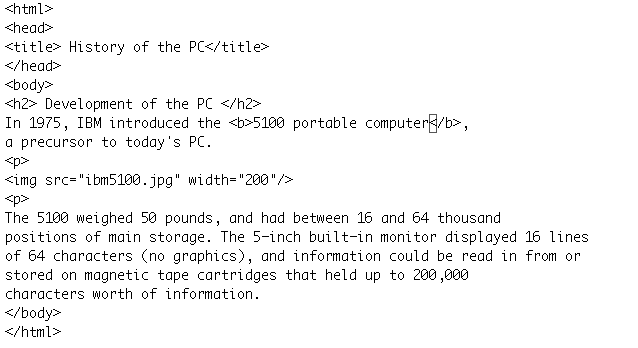
\includegraphics[width=5in]{computerIntro/images/htmlScreenshot.png}
\\
\\
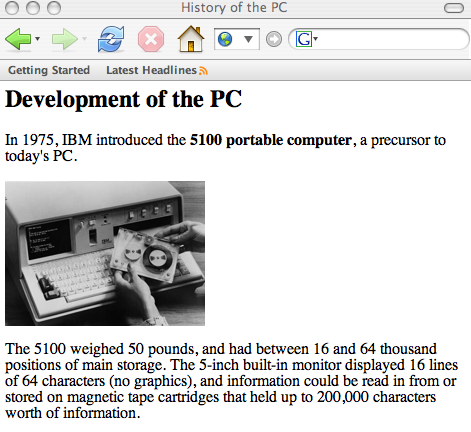
\includegraphics[width=5in]{computerIntro/images/browserScreenshot.png}
\end{tabular}
\caption{The plain text file (top - view from a plain-text editor)
  includes Hypertext Markup (HTML) which a browser software such as
  Firefox can read and display (bottom).  By simply resizing the
  browser window the line-breaks in a paragraph of text can change.
  Note that the jpeg image is not contained in the html file, only a
  reference to it.}
\label{fig:htmlBrowser}
\end{center}
\end{figure}
\end{comment}

\subsection{Identifying files}
Different file formats are designed to store different kinds of
digital information, such as documents, images, videos, and music. The
computer needs to be able to understand that a particular collection
of bytes represents a text document, an image, or a musical recording
in order to properly display it, edit it, print it, or play it.
Naming conventions have been established to make it simpler for
software to identify a file's format.  The file-name extension is
tacked on to the end of a file's name, and consists of a period
followed by a few letters (usually three) that identify the format.
For example, a plain text file will have a file extension of ``.txt'',
a CSV file will end with ``.csv'', a PDF file ends ``.pdf'', an HTML
file has either the extension ``.html'' or ``.htm'', an Excel
spreadsheet ends with ``.xsl'', and a Microsoft Word document ends
with ``.doc''.  Note that this handy convention can be ignored or
circumvented because it is possible to rename a file to a different
extension or to drop the extension without changing the contents of
the file.

Some file formats use a ``signature'' inside the file in order to
determine how to interpret the bytes of information. For example, the
beginning of a PNG file contains information that identifies it as a
PNG formatted image.  That is, the file begins with an 8-byte
``signature'', which contains the letters ``PNG'' and 2 newlines,
among other things.  If displayed in a plain text editor, it appears
as follows.
\begin{verbatim}
  ~IPNG^M
  ^Z
\end{verbatim} 
Once a program recognizes that a file has a PNG signature then it will
know how to interpret the rest of the file.  The PNG format for images
is a structured series of chunks.  Each chunk contains information on
its size and type, along with its data.  The chunk types are either
critical or ancillary, meaning that a program that encounters an
ancillary chunk can safely ignore it.  This chunk-based structure is
designed to allow the PNG format to be extended while maintaining
compatibility with older versions.

Another image format, GIF, has a signature that begins with the ASCII
representation of GIF87a or GIF89a.  Other formats also use a
signature or ``magic number'' that is stored inside the file to
uniquely identify its format.  Below are the signatures for postscript
and PDF formats, respectively.
{\footnotesize{
\begin{verbatim}
%!PS-Adobe-2.0
%%Creator: dvips(k) 5.92b Copyright 2002 Radical Eye Software
%%Title: DataTypes.dvi
\end{verbatim}

\begin{verbatim}
%PDF-1.4
3 0 obj <<
/Length 153
/Filter /FlateDecode
\end{verbatim}
}}

\subsection{Organizing Files}
Most computers organize files into hierarchies using folders or
directories. Each directory can contain an arbitrary number of files,
as well as other directories, which are referred to as
subdirectories. Subdirectories can contain files and subdirectories as
well. The system of directories and files makes a tree
structure. Figure~\ref{fig:tree} shows a tree representation of a file
system that has four levels. In this figure directories are
represented by squares and files by circles. The top of the tree is
the root directory, denoted by ``\verb+/+''. It contains all of the
files and directories.

Naming conventions for directories are the same as for files.  The
full path name of a file includes the hierarchy of directories that
contain the file.  For example, the full path name of the file
\File{X} within the directory \Directory{C} is \File{/A/C/X}, whereas
the full path name of the file \File{X} within directory \file{D} is
\File{/A/B/D/X}.  Files must be uniquely named, and although there are
three files with the name \File{X} in this directory structure, they
are uniquely named because their full path names are distinct.

\begin{figure}
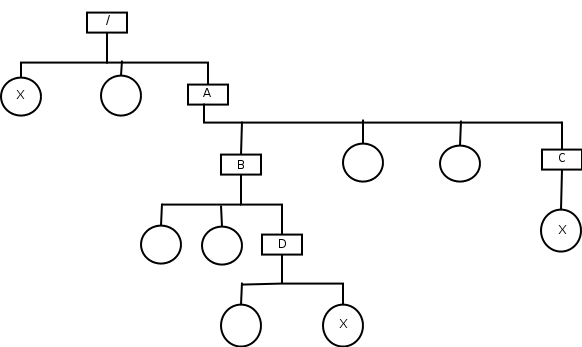
\includegraphics[width=5in]{computerIntro/images/fileTree.png}
\caption{A file system is represented here as a tree structure.  All
  of the symbols at the same level in the tree are in the same level
  of the directory structure.  Rectangular symbols represent
  directories and circles files.  Notice that there are three files
  with the name of $X$, however as they are in three distinct
  directories they are uniquely named (and so defined).  Their full
  pathnames, from top to bottom, are /X, /A/C/X and /A/B/D/X.}
\label{fig:tree}
\end{figure}

Files may also be referred to by relative path names.  For example,
relative to directory \Directory{A}, the file \File{X} in
\Directory{C} is referred to as \File{C/X}, and relative to
\Directory{A}, the file \File{X} in the top-level directory is
referred to as \File{../X}.  Here the two periods means go up one
level to \Directory{A}'s parent directory.  Users typically have a
default relative path, such as \Directory{/home/nolan/}, which can be
referred to as \verb+~+.  Hence \verb+~/+\Directory{A/C/X} is short
hand (a relative path name) for \Directory{/home/nolan/A/C/X}.

In the Windows operating system, pathnames use the backslash rather
than the forward slash.  Also, in general, file names must follow the
naming conventions required of the operating system. In most systems,
the forward slash and backslash characters, \verb+/+ and \verb+\+, are
forbidden in a name as they would be confused with directory
names. How systems handle upper and lower case varies.  For example
Unix file systems are usually case sensitive and allow user-level
applications to create files whose names differ only in the case of
characters. Whereas, Mac OS X preserves case when a file is named, but
is generally case insensitive.


\section{Components of a computer}\label{sec:components}
Most of us treat computers as black boxes that we provide input to and
get output from, and don't care about how they work. However, given
the implications of processing speed, memory, and storage on our
ability to perform scientific computations, it is good to understand
the basic structure of a computer so that we have a sense of its
limits, and so we can fix simple things and recognize potentially more
serious problems.

A computer is a general-purpose information processing machine.  For
example, the computer can display a movie for you to watch that is
stored on a DVD, or it can transfer a copy of an Excel file from a
memory stick to its hard drive for later computations.  There are many
ways to get information into a computer.  It takes input through
devices such as a keyboard and mouse, and it receives information via
a microphone or a stylus and tablet.  The keyboard, mouse, microphone,
and tablet are all known as input devices.  Information is also input
to a computer via removable storage devices, such as a compact disc
(CD), digital versatile disc (DVD), and memory stick, and from
permanent storage devices, such as a hard disk.  The Internet is yet
another means for the computer to obtain information.

The computer also gives us information.  That is, we receive
information from a computer via output devices.  We can look at a
photo on a monitor, read a news article printed to a printer, and
listen to music on the computer's speakers. The computer can also
store information on external output devices; e.g. it can store
digital information on a hard disk; it uses a CD or DVD drive to write
information to CDs and DVDs; and it can send information over the
network to another storage device.

Aside from these input and output devices, the ``guts'' of the
computer that processes information are in the ``box'', i.e. the
laptop, desktop ``tower'', or rack-mounted box.  Inside this box there
are just a few components -- the motherboard, Central Processing Unit
(CPU), Random Access Memory (RAM), hard drive and disk drive.

\begin{figure}
\begin{center}
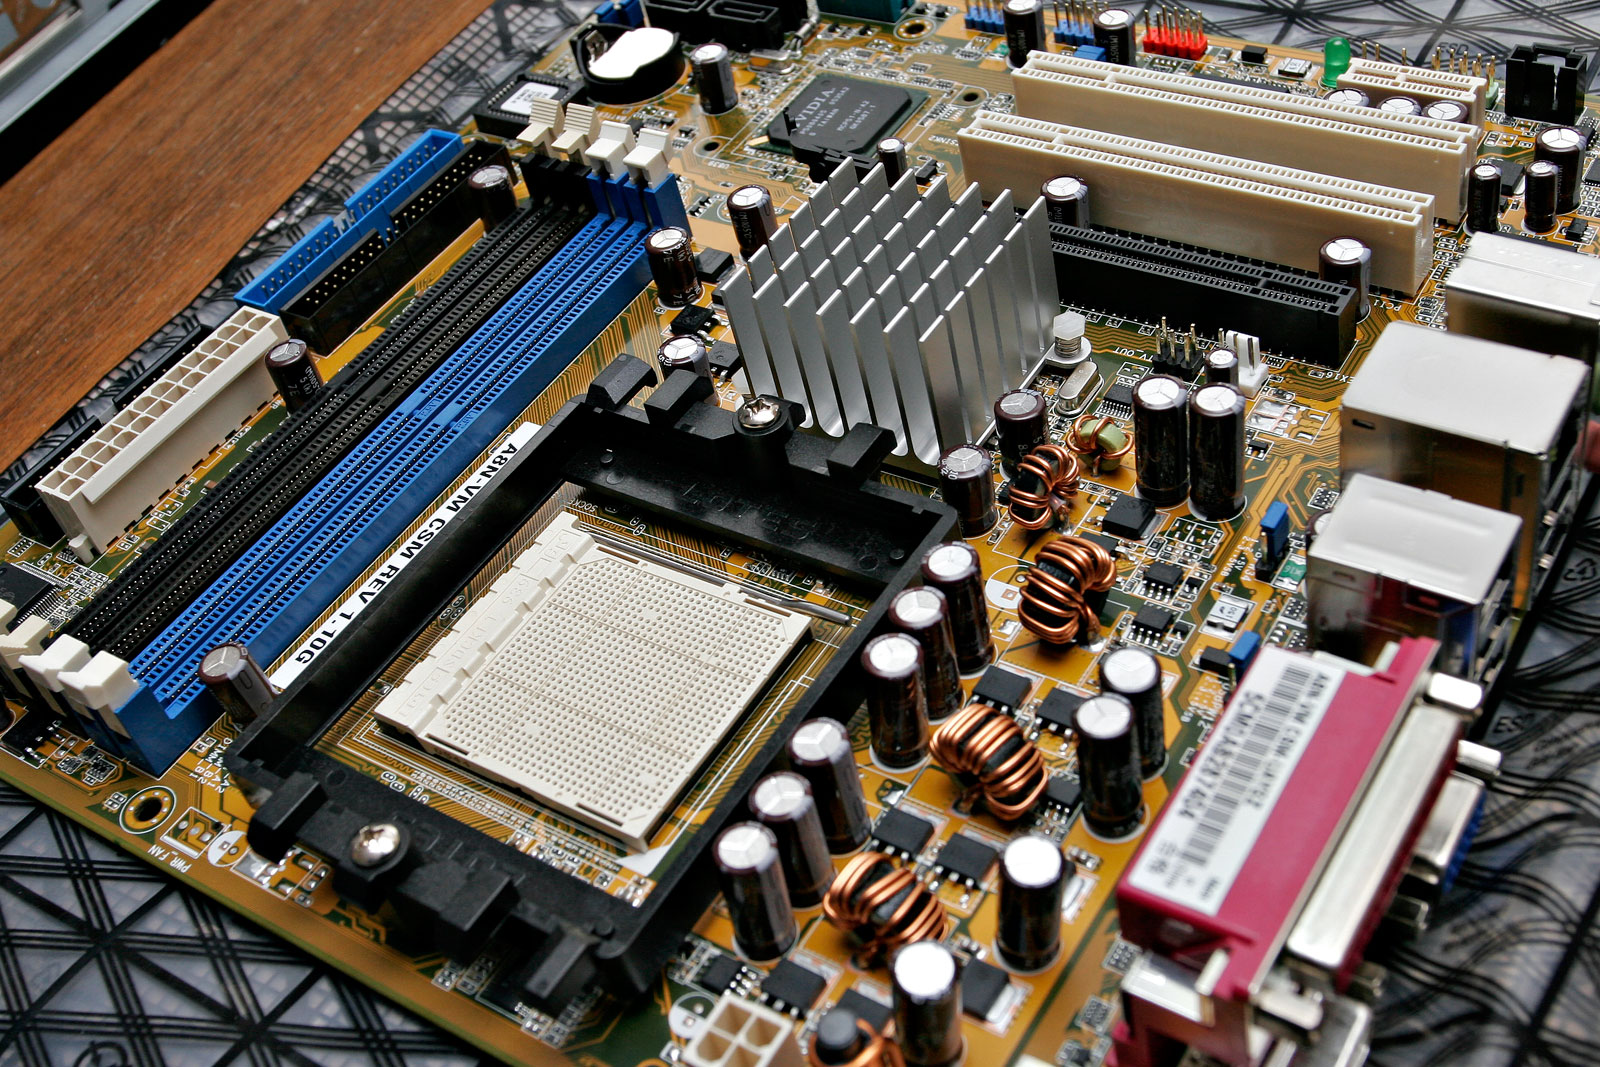
\includegraphics[height=3in]{computerIntro/images/motherboardHiRes.jpg}
\caption{The motherboard of a computer.}\label{fig:thinkpad}
\end{center}
\end{figure}

\subsection{Motherboard} The \Key{motherboard} is the physical board
that connects the internal components and also provides connectors
known as ports for the external devices.  The chips for the CPU are
plugged in or soldered to the motherboard, memory cards and video
cards are plugged in via slots, and a printer, keyboard, and internet
connection are made available via ports on the motherboard.  In other
words, the motherboard provides a common electrical and communication
system for all of the devices and internal components.  It contains
several layers that are sandwiched together.  The layers responsible
for the communication system carry data via busses, while other layers
carry voltage for the common electrical system.

\subsection{Central Processing Unit} The \Key{CPU}, also called the
microprocessor chip, is the heart of the computer.  The chip is an
integrated circuit made of transistors and capacitors that hold a
complete computation engine.  This computation engine consists of
fairly simple digital logic techniques -- it can add, multiply, fetch
a value from memory, store a value into memory, and do several other
primitive things.  More complex computations can be done in software
by combining different primitive instructions to get new, higher-level
commands.

Clock cycles are used to coordinate the actions of the transistors, so
how fast an instruction is performed depends on the chip's clock
speed. The Pentium 4 microprocessor is very fast; its clock speed is
over 3 GigaHertz (see Table~\ref{fig:HowStuffWorks}) -- that's over
three billion clock cycles per second.  Different chip designs allow
different instructions to execute natively on the circuit.  For
example, the instruction set for a Pentium chip is different from that
of the Mac G4 processor.  The G4 processor is based on RISC (Reduced
Instruction Set Computer) technology, while the Pentium 4 uses CISC
(Complex Instruction Set Computer) technology.  RISC technology has
fewer commands than CISC (about 50 compared to a few hundred), but
these commands require fewer clock cycles per instruction. This means
that the RISC processor can typically carry out more instructions in
one clock cycle than a CISC processor, e.g. the G4 can complete one
double-precision calculation every clock cycle, while the Pentium 4
cannot.  For this reason, although the G4 processor runs at only about
half the clock speed of the Pentium, clock speed does not provide a
straight forward comparison of their computational speeds.  In
addition, other factors affect computational speed such as the number
of transistors on a chip, the bus speed for moving data, and memory
size.



\begin{comment}
\begin{table}
\begin{center}
\begin{tabular}{lrrrrrr}
\textbf{Name} & \textbf{Date} & \textbf{Transistors} & \textbf{Microns} & \textbf{Clock speed} & \textbf{Data width} & \textbf{MIPS}\\
\hline
8080 & 1974 & 6000 & 6 & 2 MHz & 8 & 0.64\\
8088 & 1979 & 29000 & 3 & 5 MHz & 16 & 0.33\\
80286 & 1982 & 134000 & 1.5 &  6 MHz & 16 & 1\\
80386 & 1985 & 275000 & 1.5 & 16 MHz & 32 & 5\\
80486 & 1989 & 1200000 & 1 & 25 MHz & 32 & 20 \\
Pentium & 1993 & 3100000 & 0.8 & 60 MHz & 32 & 100\\
PentiumII & 1997 & 7500000 & 0.35 & 233 MHz & 32 & 300\\
PentiumIII & 1999 & 9500000 & 0.25 & 450 MHz & 32 & 510\\
Pentium4 & 2000 & 42000000 & 0.18 & 1.5 GHz & 32 & 1700 \\
Pentium4x & 2004 & 125000000 & 0.09 & 3.6 GHz & 32 & 7000\\
\end{tabular}
\caption{The Intel microprocessor has become much faster, smaller, and
  more powerful in the past thirty years, as seen by several measures.
  From left to right, these measures are the number of transistors on
  the chip, the width in microns of the smallest wire on the chip, the
  clock speed (number of cycles per second), the number of bits used
  for addressing data in RAM, and millions of instructions per second.
  The plot in Figure shows a comparative picture of the changes in
  these variables over time. These data are from
  \texttt{http://computer.howstuffworks.com/microprocessor1.htm}}
\label{tab:chip}
\end{center}
\end{table}
\end{comment}
   

\subsection{Memory}  
For the microprocessor to perform an instruction, the information it
requires is brought to the chip and placed directly in its
registers. The inputs to and the outputs from an instruction are very
simple values such as numbers, logical values, etc. They move to and
from the registers to a local piece of memory on the chip for
immediate reuse. The CPU has limited space in this memory cache for
storing values for the next command, and when the cache gets full,
this information is moved to bigger areas of memory, namely Random
Access Memory (RAM).

\subsubsection{Random Access Memory}
The read/write speed of RAM is much faster than a hard drive, and
unlike the technology of the hard drive, RAM technology is geared
toward accessing small pieces of data at a time.  For these reasons,
it is much faster to have the data that the CPU needs for a
computation available in RAM rather than leaving it on a storage
device such as the hard disk or a DVD.  (Random access memory is
considered ``random access'' because any memory cell can be accessed
directly if you know its location.)

Similar to a microprocessor, RAM is a chip, which is an integrated
circuit made of transistors and capacitors. In its most common form,
dynamic RAM, a transistor and a capacitor are paired to create a
memory cell.  The transistor acts as a switch that lets the cell be
read or changed. A capacitor is like a small bucket that stores
electrons. However, capacitors are leaky, and in a matter of a few
milliseconds a full capacitor loses its charge.  Therefore, the
``full'' capacitors must be constantly recharged. When the computer is
turned off, the charge in the capacitors is lost, and the contents of
RAM is gone.

In addition to this volatile dynamic RAM, a computer often has static
RAM as well.  This supply of memory has a direct connection to the
CPU, and never has to be refreshed, which makes it significantly
faster than dynamic RAM.  However, because it has more parts, a static
memory cell takes up a lot more space on a chip than a dynamic memory
cell, and that makes static RAM a lot more expensive.

Computers are often classified by the number of bits they can process
at one time, as well as by the number of bits used to represent
addresses in their main memory (RAM).  The number of bits used by a
computer's CPU for addressing information represents one measure of a
computer's speed and power.  Computers today often use 32 or 64 bits
in groups of 4 and 8 bytes, respectively, in their addressing.  A
32-bit processor, for example, has 32-bit registers, 32-bit data
busses, and 32-bit address busses. This means that a 32-bit address
bus can potentially access up to $2^{32} = 4,294,967,296$ distinct
memory cells (or bytes) in RAM. Whereas a $64$-bit processor can
access $2^{64}$ memory cells, which means the computer will be faster
with computations that require a lot of memory. Memory and data
capacity are commonly measured in kilobytes ($2^{10} = 1024$ bytes),
megabytes ($2^{20} = 1,048,576$ bytes), or gigabytes ($2^{30} =
1,073,741,824$, about 1 billion bytes). So a 32-bit address bus means
that the CPU has the potential to access about 4 GB of RAM.

\subsubsection{Virtual Memory}  
When RAM gets full, information is moved from RAM to a temporary area
on the hard drive, called the swap area or virtual memory.  The
computer manages the memory needed for computations.  It looks at RAM
for areas that have not been used recently by the CPU and copies these
areas onto the hard disk in an area set aside for temporary
storage. This frees up space in RAM to load new data. The temporary
area on the hard drive is called virtual memory because the copying
described here happens automatically and makes your computer act like
it has unlimited (or really large) RAM space. However, virtual memory
is much slower than RAM.  When performing computations there is a
trade-off between RAM and speed: the more information we hold around,
i.e. the more memory we use, the faster computations are.

\subsubsection{Read-only Memory} 
Read-only memory (ROM), also known as firmware, is an integrated
circuit programmed with specific data when it is manufactured.  This
memory is used to store the initial instructions the computer needs to
start. When we turn on a machine, it ``boots'' up which means that it
bootstraps itself into activity. It does this bootstrapping using its
BIOS (Basic Input/Output System) located in ROM.  The BIOS
instructions do things like test the hardware of the machine. In
general, it provides a very low-level interface to the different
components of the machine and the peripherals.  This bootstrapping
step initializes the components and gets the machinery into working
condition, and then tries to find the operating system to which it
will pass control.  This operating system might be Windows, MacOS X,
Linux, BSD or some other system.  It might be located on (one of) the
hard drive(s), on a CD or even on another machine.


\begin{comment}
  ??With the tremendous growth in information stored on disks,
  computer scientists have started to conduct studies of the
  reliability of disk drives. Recently, Google engineers studied their
  disk drive population where they examined disk failures for
  approximately 100,000 hard drives over an eight month period. They
  found some surprising results.  For instance, it appears that
  failures do not correlate with temperature.  Also they found that
  while scan errors are associated with increased chance of disk
  failure, the detection of the first scan error affects the chance of
  survival differently for newer drives in comparison to older
  drives. The younger drives, the chance of failure increase sharply
  within the first month after the scan error is detected and then
  flatten out, whereas for the older drives, the failure rate steadily
  increases throughout the observed eight months. (See
  Figure~\ref{fig:googleDriveFailure}.)

\begin{figure}
\begin{center}
PUT FIGURE HERE
\caption{The survival rate of disk drives in the eight months after
  the first scan error.  The disk drives are grouped according to the
  age at the time of the scan error. The curve for the younger drives
  ($0-8$ months old) drops sharply in the month after the first scan
  error and then levels out at about 90\%.  In comparison, the drives
  that are at least two years old, drops even more sharply in the
  first month and then continues to decline
  steadily.}\label{fig:googleDriveFailure}
\end{center}
\end{figure}
\end{comment}


\subsection{Operating System} The operating system, and specifically
the kernel, is essentially a regular application that manages the
resources of the machine. The kernel is run when the operating system
is started and it can start other applications, allocate resources to
these applications and basically coordinates access to the disks, file
systems on the disks, network connectivity, screen, memory, and so on.
At the simplest level, an operating system does two things:
\begin{itemize}
\item It manages the hardware and software resources of the computer
  system.  These resources include such things as the processor,
  memory, disk space, etc.  The operating system makes sure that each
  application gets the necessary resources and shares these resources
  with the other applications running on the computer.

\item It provides a stable, consistent way for applications and users
  to deal with the hardware without having to know all its details.
  That is, the operating system provides a consistent application
  interface and user interface, no matter what particular type of
  computer it is running on.
\end{itemize}

A consistent application program interface (API) allows a software
developer to write an application on one computer and have a high
level of confidence that it will run on another computer of the same
type, even if the amount of memory or the quantity of storage is
different on the two machines.  Also, an operating system can ensure
that applications continue to run when hardware upgrades and updates
occur, because the operating system and not the application is charged
with managing the hardware and the distribution resources.


\subsection{Storage Devices}
Hard disks or disk drives store information magnetically on flat disks
sometimes called platters.  These disks spin very quickly as a
read/write head moves from the center to the edge of the disk finding,
reading, and writing, information.  In this way, magnetic storage can
be easily erased and rewritten, yet the disk can store information for
many years.

A compact disk stores and reads information using optical or laser
technology rather than magnetism. The CD is a plastic disk with a
smooth reflective layer on top of a photosensitive dye.  Information
is written on a CD, or burned on, with a laser that heats the dye
layer and turns it dark. The CD is read by another laser that tracks
the reflection of its beam.  The light from the read-laser reflect
back to the laser at different levels according to whether or not the
reflective layer is obscured by the darkened dye or
not. Alternatively, CDs can have information stamped on them.  These
CDs have bumps and flat regions stamped into the reflective surface;
similar to the photo-sensitive dye, the bumps reflect the light
differently than the flat spots. DVDs are like CDs but with a much
larger storage capacity.


\subsection{A Bit of History}
In 1975, IBM introduced the 5100 portable computer
(Figure~\ref{fig:5100Thinkpad}), a precursor to today's PC. The 5100
weighed 50 pounds, and had between 16 and 64 thousand positions of
main storage. The 5-inch built-in monitor displayed 16 lines of 64
characters (no graphics), and information could be read in from or
stored on magnetic tape cartridges that held up to 200,000 characters
worth of information (that's about the equivalent of all the letters
in the first three chapters of this book).  Depending on its features,
the 5100 cost from nine to twenty thousand dollars (1975 dollars).  A
little over fifteen years later, IBM launched its Thinkpad series
(Figure~\ref{fig:5100Thinkpad}).  Like the 5100, these notebooks have
a keyboard, monitor, and storage drive built into the main unit, but a
Thinkpad is a far smaller, more powerful machine than its
predecessor. For example, the 1$\times$10$\times$12 inch Thinkpad T41,
introduced in 2003, weighs only 5 pounds, has a 14-inch screen with
1024$\times$768 color pixels, and cost only \$1,500-\$3,000, depending
on the configuration. The memory available for the T41 ranges between
256MB and 2GB, about 30,000 times that of the 5100. In place of a
tape-cartridge device, information can be stored on a CD, DVD, or a
40-80 GB hard drive. Other features include things we all expect in a
laptop these days, such as a touchpad with mouse buttons, battery with
four hours of life, and built-in antenna for connecting to the
Internet.

\begin{figure}
\begin{center}
\begin{tabular}{cc}
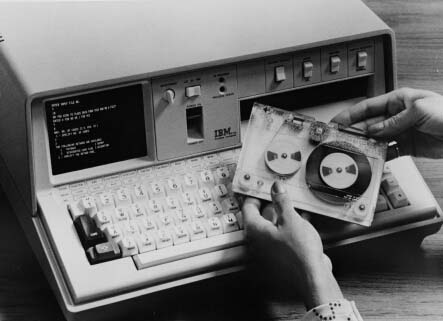
\includegraphics[width=3in]{computerIntro/images/ibm5100.jpg}
&
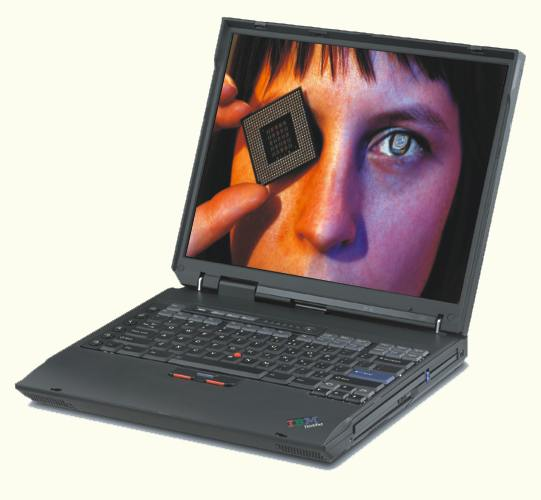
\includegraphics[height=2.2in]{computerIntro/images/ibmThinkpad.jpg}
\end{tabular}
\caption{The 5100 (left), introduced by IBM in 1975, was the precursor
  to the PC.  The keyboard, monitor, and tape drive were built into
  the unit.  Designed for engineers and scientists, it weighed about
  50 pounds and cost \$9,000 to \$20,000.  Thirty years later, IBM's
  Thinkpad laptop (right) also came with the monitor, keyboard, and
  storage device built-in.  However, it weighs only 5 pounds, has a
  hundred thousand times the memory, nearly a million times the
  storage capacity, and costs around \$2,000 in today's dollars.}
\label{fig:5100Thinkpad}
\end{center}
\end{figure}

According to the announcements at the time, the 5100 would ``put
computer capabilities at the fingertips of engineers, analysts,
statisticians and other problem-solvers.'' \footnote{IBM PC exhibit.
  http://www-03.ibm.com/ibm/history/exhibits/pc/pc$\_$2.html} Clearly,
the PCs and laptops of today have accomplished this claim and then
some.  By 2003, the year the T41 was introduced, IBM sold its 20
millionth ThinkPad. This dramatic change in computing power over the
past thirty years has indeed made a significant impact on scientific
computing. 


\begin{comment}This is an introduction to desktops, laptops, and
  mainframes; it is not an introduction to embedded computational
  devices in cars, cell phones, automated teller machines, etc.
\end{comment}


\section{Computing Languages}
The commands that we use in a programming language provide access to
complex operations.  They are built from primitive instructions that
reside on the computer chip.  These primitive instructions are
analogous to the axioms of mathematics, and programming languages
provide access to the more complex operations that are built from
these ``axioms''.  Like human languages, there are many computer
languages that have evolved in different communities with different
dialects.  These can be roughly categorized into low-level assembler
language, compiled languages, virtual machines, and interpreted
languages.  In addition there also point-and-click and drag-and-drop
interfaces to computing.


\subsection{Assembler} 
Assembler language is a very low-level, primitive language used to
specify sequences of CPU-level instructions to do a higher-level task.
The language is tied to the particular set of instructions available
on the CPU.  The assembler programmer has to do all the work,
specifying exactly what to do in the CPU's own language. For example
to perform a simple calculation such as $z = x + 3*y$ requires many
low-level instructions, such as
\begin{itemize}
\item Get value in address of $y$, put in register
\item Put 3 in register
\item Multiply, store result in register
\item Get value in address of $x$, put in register
\item Add, put result in register
\item Put result in address of $z$
\end{itemize}

The software written in assembler is often very fast to run, but on
the other hand it is slow to develop and maintain.  Most of us do not
want to worry about moving bytes in and out of CPU registers. The
high-level systems we use for working with data insulate us from the
representations of different types of numbers and from underflow and
overflow errors.  And this is where we want to be - using commands
that allow us to think in terms of the data and the statistical
problem on which we are working, and leaving the mapping of these
actions to the basic operations to the low-level computer
facilities. This is the general premise motivating programming
languages such as Fortran, C, Java, and much higher-level languages
such as S (R and S-Plus), Matlab, SAS, and other applications such as
Excel.

These languages allow people to express computations in a more human
readable and understandable way.  The instructions in these higher
level languages are translated by the language software to machine
code that the CPU can understand.

\subsection{Compiled languages}
One step above assembler are the C and Fortran languages.  Fortran
provides a higher-level mechanism to express computations involving
formulae and the language translates these formulae to machine
instructions. This is where the name Fortran comes from:
\textit{for}mula \textit{tran}slator.  The Fortran language has
evolved from Fortran 66 to Fortran 2000, which has increasingly modern
programming facilities. Because of the simplicity of the language, it
is quite fast and some argue that it is the most efficient language
for scientific computing. (This requires much greater specificity
about what efficiency means and also how to measure performance
appropriately.)  Fortran is useful, but it is clumsy and less well
suited to good software engineering than most other common languages.
However, it is very useful to be able to read and interact with
Fortran code because so much of the existing numerical software was
developed in Fortran.

The C language is a much richer language than Fortran and has been
used to implement operating systems such as Unix and Linux.  It has
been the language of choice for many years and is used widely in
numerical computing.  More recently C++ has become fashionable because
it offers many benefits over its close ancestor, C.  However, these
benefits are not without complexity.

Both Fortran and C are languages that are compiled.  In other words,
programmers write code and then pass it to another application - the
compiler - that turns it into very low-level machine instructions.
The result is an executable that can be run to carry out the
instructions.  Such executables are invariably machine-dependent,
containing machine-level operations that are specific to the machine
targeted by the compiler.  The same source code can be recompiled on
other machines, but this compilation step is necessary, and in many
cases, one must either modify the code for the new machine or be
conscious of the portability constraints when authoring the code.


\subsection{Virtual Machines}
Compiled languages, i.e. those requiring a compiler, are very
useful. Typically, the compilation step performs optimization
procedures on the programmer's code, making it faster by, e.g.,
looking at the collection of computations and removing
redundancies. Additionally, because compiled languages typically
require variable declarations in terms of scope and type information,
they can often catch programming errors before the code is run.  

\begin{comment}
%This appears earlier
There are disadvantages, however.  Using compiled languages, one
typically has to write an entire program before compiling it.  This
means that

\begin{itemize}
\item exploration and rapid prototyping of individual chunks is more
  complex or impossible. Specifically, it is much more difficult to
  incrementally create software by running individual commands.
\item one cannot typically alter the programming as it is running to
  correct errors or add functionality.
\end{itemize}
\end{comment}

The C++ language is in some sense an object-oriented extension of
C. It is a compiled language that allows for greater code reuse and
better software engineering for extensibility.  From our perspective,
C++ is still a low-level, compiled language that is analogous to C.

Java and C\# are very similar languages that one can categorize as
being simplified variations of C++ that promote the object-oriented
style of programming but without the complexity of C++.  They are also
compiled languages, requiring a separate compilation step.  Unlike C
and Fortran compilers, the Java and C\# compilers transform the
programmer's code into higher-level instructions targeted at what is
termed a Virtual Machine (VM).  The VM acts much like a computer,
processing the instructions, providing registers, etc. and generally
mimicking the actions of the low-level computer. This is done by
creating a version of the virtual machine for each computer
architecture (e.g. Powerbook, Intel *86, Sparc), but then allowing all
code for that virtual machine to run independently of what machine it
is running on. The virtual machine is a layer between the compiled
code and the low-level computer. And this makes the compiled code
(byte code) independent of the particular architecture and so makes it
portable without the need for recompiling.


\subsection{Interpreted languages}
Instead of compiling source code into machine code, other languages
read and interpret the code dynamically.  That is, the language has an
interpreter that parses and evaluates the code as it finds it, one
command at a time.  The interpreter is often called a Virtual
Machine. It emulates the real machine, providing software
implementation of the higher-level constructs we need.  For example,
loops and iterations; conditional execution and branching; and
variables.  The virtual machine is, for example, itself written in C
and compiled, but it can run arbitrary code for that language.  This
emulation makes interpreted languages generally slower than compiled
ones. Examples of interpreted languages include: Java, Perl, Python,
R, S-Plus, Matlab, Octave, and SAS. Java and Perl first create
``byte-code'' to speed up interpretation, although they still use a
virtual machine.

The acronym Perl stands for Practical Extraction and Report Language.
Perl is designed for text processing, and as such, it is extremely
fast at text manipulation.  The arcane constructs of the language make
it easy to create very terse programs. Although this may be beneficial
when programming, it tends to be challenging when debugging or reading
code a short time later.  Some dislike the language from a software
engineering perspective, but love it for its practicality.  Similar to
Perl in concept and purpose is the interpreted language Python.
Python is much more elegant than Perl because it was developed from an
object-oriented perspective, unlike Perl where the object-oriented
capabilities were added on. Python does not have as many add-ons as
Perl-yet.
% The syntax of the language uses white space to identify
``stanzas'' or blocks in the code.

The interpreted languages such as R, S-Plus, Matlab, and Octave are
aimed at a specific audience, e.g. statisticians, engineers, and they
provide higher-level functionality that the audience would find
useful. These are written in C and made available through libraries or
toolboxes of ``routines'' that build on the core language.  (C has
very few built-in functions that statisticians and engineers want.)
Thus the trade-offs for the slower speed are the higher-level
language, the specialized functionality, and portability.

\begin{comment}
\subsubsection{Java} Java is a language, a Virtual Machine Interpreter
and a collection of libraries.  The language object oriented, and is
similar to C++ in syntax, but without many of the error-prone elements
of C++ related to garbage collection and memory management.  Java
provides support for parallel processing with threads. It is a very
portable language, but requires a VM for each platform/Operating
System.  Java can be used in Web pages, and it provides secure
computations in distributed environment.
\end{comment}

R and S-PLUS have a nearly identical syntax that is
based on the $S$ language.  They were developed by and for
statisticians, and are constantly evolving as the large community of
researchers provide add-ons that bring new statistical methodology to
the users.  R and S-plus are the de facto standard for statistical
research and non-standard analyses.

As a simple comparison of R and the lower-level C language, imagine we
have a vector of numbers $x$. In C or C++, to get the sum of the
values in $x$, we write the following code.
\begin{verbatim}
double total = 0;
int j; int n;
double x;
for (j=0; j<n; j++){
    total += x[j];
}
\end{verbatim}
In comparison, in R, we write \RCode{sum(x)}.

Matlab is a commercial interpreted language designed for
engineers.  It is remarkably fast performing linear algebra and
numerical modeling algorithms.  Matlab is a simple, general
programming language, but it has little support for high-level
statistical concepts, such as models and categorical data.  Octave is
an open source language that is mostly compatible with Matlab.

\begin{comment}
\subsubsection{SAS}
Systems or environments like SAS provide either a batch or interactive
interface.  The interactive interface supports exploratory,
interactive data analysis, but it does not allow the programmer to
readily manage the intermediate results from each step and put them
into the next steps and generally branch in different directions.  The
BATCH system allows us to do interactive work in very coarse-grained
increments; run these sequence of commands on this data and produce
this output. Then, look at the output and write some more code. While
superficially this is the same sequence of steps in EDA that we might
do in R, the interface is much less convenient.
\end{comment}

\subsection{Excel and JMP}
The point-and-click, drag-and-drop interfaces like the one provided by
Excel and in SAS' JMP are very useful for specific tasks such as
editing values in cells, quickly creating plots, etc.  Managing
results and output from different tasks (e.g. regression, ANOVA,
summary statistics) across sheets can be hard work.  The visual
interface which is the thing that makes Excel, and graphical user
interfaces (GUIs) in general, convenient is a hindrance here.  While
we can put different results in their own worksheets, this soon gets
cluttered and we spend time navigating the tabs in the workbook.
Another complexity in this world of point-and-click for EDA is that
specifying precisely what we mean can be difficult.  In some cases, we
might want to customize a particular methodology when applying it to
data, or we might want to draw a plot slightly differently, or use a
data set that we derive in a complex way from the original source.  For
these common but non-standard situations, a sequence of dialogs
provided by a ``wizard'' can be frustrating.  It is tediously long,
especially if we are doing it several times with different subsets of
the data or different data sets that we wish to compare.  In addition
to the unnecessary repetitiveness, we also cannot specify everything
we may want to. The dialogs provide access only to the common
options. In the interest of keeping them simple, the designers have
identified what they believe are the important elements a user can
specify and change.  It is not possible for us to create our own
modifications of these tasks, or at least it is a major project to do
so.


\setcounter{chapter}{2}
	
\chapter{The R Programming Language}
\label{chap:RIntro}
This chapter introduces some of the core ideas in the R programming
language and environment and shows how to use it. We provide a broad
picture of the language rather than an exhaustive view.  The aim is to
uncover the rationale of the language. R is a terrific, interactive
medium with which you can hypothesize and test characteristics, and we
expect the reader to explore the ideas interactively using the R
environment as they read this chapter and experiment with how the
language works. Finding out how R works and learning to think about
how to express computations in R will greatly simplify your future
work. It is good to take the time early on to learn a language and not
simply use it in a utlitiarian, ad hoc manner. While R is a specific
language that you may or may not use extensively in the future, it is
important to realize that what you learn when exploring R will be
generally applicable to many different programming languages that you
might use.


\section{Getting Started}
We first start R by invoking the command \verb+R+ at the command line
or by launching the R user interface.  
{\footnotesize{
\begin{verbatim}

R version 2.7.1 (2008-06-23)
Copyright (C) 2008 The R Foundation for Statistical Computing
ISBN 3-900051-07-0

R is free software and comes with ABSOLUTELY NO WARRANTY.
You are welcome to redistribute it under certain conditions.
Type 'license()' or 'licence()' for distribution details.

R is a collaborative project with many contributors.
Type 'contributors()' for more information and
'citation()' on how to cite R or R packages in publications.

Type 'demo()' for some demos, 'help()' for on-line help, or
'help.start()' for an HTML browser interface to help.
Type 'q()' to quit R.

[Previously saved workspace restored]
> 
\end{verbatim}
}}
Note the line that says:
\begin{verbatim}
[Previously saved workspace restored]
\end{verbatim}
This means that R is loading up the data that was saved from the
last R session.

R is both an interactive and interpreted language. By interpreted, we
mean that we can give an instruction and immediately have it
evaluated. Then, we can give another command.  R has lots of functions
(over 1500 immediately available to you and thousands more in add on
packages). It is impossible to remember all of these and their details
(e.g. what arguments they take, what they do in all situations and
what they return) and to make effective use of R, you need to get into
the habit of using the help system. (One way to get help is to type
\verb|help("topic")| to get help on the specified topic.)

In this chapter we present the basic building blocks in R that you
have available to you.  R is a programming language that is
statistically focused. It is a good tool to know for doing any kind of
data analysis. To use it effectively, you will need to understand
these basics and to gain experience with the engine and the numerous
functions.

One way to use R is as a heavyweight calculator. 
\begin{verbatim}
> 1+2
[1] 3
\end{verbatim}
Like a calculator, R has built-in values, such as \SVariable{pi}. 
\begin{verbatim}
> 1+pi
[1] 4.141593
\end{verbatim}   
In R, the \SVariable{pi} ``thing'' in this computation is a
variable. By this we mean it is a name by which we refer to a
value. We can associate new values with this name by
{\em{assigning}} a value to it. For example, we can give
\SVariable{pi} the value 1 and then use that.
\begin{verbatim}
> pi = 1
> 1+pi
[1] 2
\end{verbatim}
So \SVariable{pi} is not a constant in this world. Mathematically, it
is, but in the programming world, it is merely a variable to which we
can bind or assign new values. Of course, this is not necessarily a
good idea. If we use this new value for $\pi$, we will get strange
results!

There are several ways to assign a value to a variable in R. They
differ only in syntax.
\begin{verbatim}
> x = 1+2
> x <- 1+2
> 1+2 ->x
> x
[1] 3
\end{verbatim}
These three forms (=, \textless{}-, and -\textgreater{}) can all be
used, however the last is very rarely seen. It arose when one was
typing a long command and realized that we had forgotten to assign the
result. At one time, we couldn't go back to the beginning of the line
without deleting all the intervening text and so removing the
command. Nowadays, we can jump to the beginning of the line, and add
the assignment and continue on. In reasonably recent versions of R,
one could also use the underscore (\_) as the assignment
operator. This is no longer possible and soon we will be able to use
it as a character in a variable name. So the following error occurs
when we try to assign using \_ now:
\begin{verbatim}
> x_ 1
Error: syntax error
No suitable frames for recover()
\end{verbatim}


Now that we can create variables, we can do some useful things, and we
may want to ensure that we don't lose anything we do. It is a good
time to think about how we might save our data. Each time we run R, we
create a new R session. Then we can do some work, create new variables
and potentially want to save some or all of them. We can save our
entire workspace, i.e. all the variables we have created calling the
function the \SFunction{save.image} at any time. This puts all the
objects in our session workspace into a file named .RData. If we
start R again (in that directory), the contents of that .RData are
loaded into the new session and are immediately available to us
again. If we start in a different directory, we can still load the
values into the R session, but we must do this ourselves using the
function \SFunction{load} and giving it the fully qualified name of
the file to load (i.e. full directory path and file name).

When we end the R session using the \SFunction{q} function, we will
normally be asked whether we want to save the session or not. This
calls \SFunction{save.image} implicitly.

If we don't want to store all the variables, but only specific ones,
we can explicitly \SFunction{save} one or more objects to a file (or
generally a connection). This is convenient when we create a big
dataset and then want to ensure that it gets saved before we do
anything else. Or if we want to make an object available to another R
session, e.g. to somebody we are working with, without terminating
ours, we can simply write the object to disk and then send it that
person in an entirely portable format.

Note that R uses "copying" semantics. When we assign the value of
\Svariable{x} to \Svariable{y}, \Svariable{y} gets the value of
\Svariable{x}. It is not ``linked'' to \Svariable{x} so that when
\Svariable{x} is changed, \Svariable{y} would see that
change. Instead, we copy the value of \Svariable{x} in the assignment
and the two variables are unrelated after that.
\begin{verbatim}
> x
[1] 3
> y = x
> x = 10
> x
[1] 10
> y
[1] 3
\end{verbatim}
We have seen how we can store the results of computations or simple
values in variables. We can think of these as being stored in our
workspace. This is like our desk with pieces of paper storing
different information. We would put different pieces of paper in
different places so that we can easily find them again when we need
them. The place we put them allows us to quickly find them and is
analogous to the variable name which allows us to easily refer to the
values.

In the same way that we might overload our desk with pieces of paper
as we move from task to task, or just have too much information, we
need to manage the variables we have in our work area or desktop. R
provides functions which we can use to dynamically manage the
variables and the contents of our workspace. The function
\SFunction{objects} gives us the names of the variables we have in our
workspace.
\begin{verbatim}
> objects()
[1] "x"  "y"  "pi"
\end{verbatim}
We can remove values using \SFunction{remove} by passing the name to
the function of the variable we want to remove.
\begin{verbatim}
> remove("x")  
\end{verbatim}
and we can verify that the variable has been removed using
\SFunction{objects} again.
\begin{verbatim}
> objects()
[1] "y"  "pi"
\end{verbatim}
We can give more than one name. So we can remove both \SVariable{y}
and \SVariable{pi}, the last two remaining variables in our
session's workspace.
\begin{verbatim}
> remove("y", "pi")
\end{verbatim}
Before we leave this topic, we should ask what happened to the
original version of \SVariable{pi}? We assigned a new value to it - 1
- and used that in our computations? Now that we removed it, is
\SVariable{pi} defined at all?  Is the old value put back? The answer
is that the old value is now in effect again, but it wasn't ``put
back''. R did not remember the old value and restore it when we removed
our version of \SVariable{pi}. The explanation is a little more
complicated, and a lot richer. It relates to where we were finding the
variable named \SVariable{pi}.

When we issued the command 
\begin{verbatim}
> pi = 1
\end{verbatim}
we were telling R to associated the value 1 with the variable name
\SVariable{pi}. This puts it in our workspace. But before we did this,
we managed to find \SVariable{pi} also, and then it had the usual
value of 3.141. So where did it come from? It wasn't in our workspace,
yet it was still available.

The answer involves understanding how R finds variables when we refer
to them. R actually keeps a collection of places in which to search
for variables. This is called the search path. This is an ordered
collection of workspaces containing variables and their associated
values. At any point during an R session, we can ask R what this
collection of workspaces is. We do this using the function
\SFunction{search}. In this session, we get
\begin{verbatim}
> search()
[1] ".GlobalEnv"     "package:Rbits"    "package:methods" 
[4] "package:stats"  "package:graphics" "package:utils" 
[7] "Autoloads"      "package:base"    
\end{verbatim}
The first entry is our own personal workspace. When we quit, this
disappears. The other entries are packages or libraries of functions
and data that are available to us.

Now, when we implicitly cause R to look for a variable, it walks along
this collection and asks each entry whether it has the relevant
variable. After we defined our own version of \SVariable{pi}, when we
used \SVariable{pi} in a computation such as \verb|1 + pi|, R started
its search for \SVariable{pi}. It started in the first element of the
search path, and found it there. That is our workspace where put
\SVariable{pi}.

 When the session started and we did not yet have our own version of \SVariable{pi}, the search for \SVariable{pi} was rather different. R looked through each element of the search path and found \SVariable{pi} only in the last entry "package:base". This contains the built-in variable provided by the R system itself (rather than add-ons). 

 How could we know where R would find a variable? We can use the function \SFunction{find}. So in the following, we define \SVariable{pi}, and ask R where we can find it. 
\begin{verbatim}
> pi = 1
> find("pi")
[1] ".GlobalEnv"   "package:base"
\end{verbatim}
Now, we remove our version of \SVariable{pi} and then R can only find the one in "package:base". 
\begin{verbatim}
> remove("pi")
> find("pi")
[1] "package:base"
\end{verbatim}
All the functions we have seen so far, and in general, are simply
values assigned to variables. R finds them in the same way when we
refer to them in a computation. It looks through the search path until
it finds the variable. It is slightly smarter for functions. If it
knows we are calling the value of the variable as a function, it will
only look for a function, skipping over other types of values.

What if we look for a variable that doesn't exist? For example,
suppose we use a variable named \SVariable{fred} in a computation
\begin{verbatim}
> fred^2
\end{verbatim}
What happens? R looks through each element of the search path and
eventually gives up, giving the error message:
\begin{verbatim}
Error: Object "fred" not found
\end{verbatim}
We can determine whether a variable is defined using \SFunction{find},
or using a more convenient function in some cases named
\SFunction{exists}. For example,
\begin{verbatim}
> exists('fred')
[1] FALSE
\end{verbatim}
(Note that you can use single or double quotes for a string,
i.e. \verb+"fred"+ or \verb+'fred'+.)


\section{The Basic Data Types}
In R, everything is an object. We have seen this already. We have
variables that refer to values, and functions which do things are
accessed as regular variables. So we see that we have a commonality
for data and functions. This is different from many languages such as
C/C++, Java, etc. For interpreted languages, it is quite common and it
is very powerful.

The basic or primitive types of objects are vectors. These are simply
collections of values grouped together into a single container. The
basic types are integer, numeric, logical and character vectors. A
very important characteristic of these vector types is that they can
only store values of the same type. In other words, a vector has
homogeneous data types. We cannot use a vector to store both an
integer and a string in their basic forms. (We'll see that we can put
them into a vector and the integer will become a string. Also, we can
use what is called a ``list'' to store them both in their original
form.)

As we just said, there are 4 basic types of vectors: integer,
character, numeric and logical. Integer vectors store integer values,
numeric vectors store real numbers, logical vectors store values that
are either TRUE or FALSE and character vectors store strings. In C and
Java, we can work on characters individually. However, in R there is
no way to store a single character except as a simple string with only
one character. This is very rarely a problem.

Essentially, vectors are like arrays in C and Java. In those
languages, there is a large difference between a scalar or basic
built-in value and arrays of such values. In R, there are no
scalars. By this, we mean that there are no individual number objects,
or logical values, or strings. Instead, such individual values are
actually vectors of length 1. So they are special cases of general
vectors with multiple elements. This makes lots of computations
convenient.

An important function for creating vectors is the \SFunction{c}
function. The `c' stands for concatenate, and all it does is take one
or more values and put them into a new vector. For example,
\begin{verbatim}
> c(1.2, 4.5, 3.2)
[1] 1.2 4.5 3.2
> c(TRUE, FALSE, FALSE, TRUE)
[1]  TRUE FALSE FALSE  TRUE
> c("Abc", 'def', "ghikllm", "z")
[1] "Abc"     "def"     "ghikllm" "z"      
\end{verbatim}
What about the integer vector? Well, in R, all numbers that we type
are made into real numbers. So when we type
\begin{verbatim}
> c(1, 2, 3)
\end{verbatim}
we get a numeric vector as the individual values are actually
numeric. (This is different in S-Plus, version 5 and higher.)

There are many cases in which we want integers and they arise
naturally. One of them, as we shall see in the subsetting section, is
a sequence of integers. The built-in syntax for creating the integer
sequence a, a+1, a+2, ..., b is \verb|a:b|. For example,
\begin{verbatim}
> 1:10
 [1]  1  2  3  4  5  6  7  8  9 10
> 4 : 5
[1] 4 5
> 10:3
[1] 10  9  8  7  6  5  4  3
> 3:3
[1] 3
\end{verbatim}
This is a very specific version of the more general \SFunction{seq}
function. This allows us to create sequences with different strides
(differences between successive elements), of specific length, and so
on. See the help pages.
\begin{verbatim}
> seq
function (...) 
UseMethod("seq")
<environment: namespace:base>
> seq(1, length = 10, by = 2)
 [1]  1  3  5  7  9 11 13 15 17 19
\end{verbatim}


An important characteristic of any vector is its length. We can always
find out how many elements a vector contains using the function
\SFunction{length}.
\begin{verbatim}
> x = 1:10
> length(x)
[1] 10
> letters
 [1] "a" "b" "c" "d" "e" "f" "g" "h" "i" "j" "k" "l" "m" "n" "o"
[16] "p" "q" "r" "s" "t" "u" "v" "w" "x" "y" "z"
> length(letters)
[1] 26
\end{verbatim}
Note that the return value from calling \SFunction{length} is itself a
vector. It is an integer vector of length 1. The system uses its own
built-in types to provide functionality.

Often we want to combine two vectors. We can also do this using the
\SFunction{c}.
\begin{verbatim}
> x = c(1, 2, 3)
> y = c(4, 5, 6)
> c(x, y)
[1] 1 2 3 4 5 6
\end{verbatim}
We can also use the function \SFunction{append}. Look at the help for
\SFunction{c} and \SFunction{append} and try to discover the
difference.

In many situations, it is convenient to associate names with elements
in a vector. For example, suppose we have IP addresses of machines
stored as strings. We might also want to associate the human-readable
name along with it. For example,
\begin{verbatim}
          wald          anson         fisher 
"169.237.46.2" "169.237.46.9" "169.237.46.3"
\end{verbatim}
Here, we have associated the names wald, anson and fisher with the
elements of the character vector.

For any vector, we can ask for the names of the elements. Suppose the
vector of IP addresses above was assigned to the variable
\SVariable{ip}, then we could get the character vector of names using
the function \SFunction{names}.
\begin{verbatim}
> names(ip)
[1] "wald"   "anson"  "fisher"
\end{verbatim}
If the vector has no names, we get back \textsl{NULL}. This is a
special symbol in R, and has length 0. We can check if a value is
\textsl{NULL} using \SFunction{is.null}:
\begin{verbatim}
 is.null(names(ip))
\end{verbatim}


There are several ways to specify the names for a vector (of any type,
i.e. integer, numeric, logical or character). If we are explicitly
creating the vector (using \SFunction{c}), then we can put the names
in the expression, as in
\verb|c("169.237.46.2", "169.237.46.9", "169.237.46.3")|.
\begin{verbatim}
> c(wald="169.237.46.2", anson = "169.237.46.9", 
   fisher = "169.237.46.3")
\end{verbatim}
If we already have a vector, then we can assign names to the elements
using the \SFunction{names} function (or technically the
\verb+names<-+ function).
\begin{verbatim}
> x = 1:26
> names(x) <- letters
a  b  c  d  e  f  g  h  i  j  k  l  m  n  o  p  q 
  r  s  t  u  v  w  x  y  z 
1  2  3  4  5  6  7  8  9 10 11 12 13 14 15 16 17 
 18 19 20 21 22 23 24 25 26 
> y = c(0, 0, 256)
> names(y) = c("R", "G", "B")
> y
  R   G   B 
  0   0 256 
\end{verbatim}
Useful general facilities for operating on vectors are
\SFunction{rep}, \SFunction{rev}, \SFunction{sort}. \SFunction{rep}
allows us to replicate a vector in convenient ways.
\begin{verbatim}
> rep(c(1, 2, 3))
\end{verbatim}
For character vectors, \SFunction{paste} is convenient for combining
strings together. The function \SFunction{strsplit} can be used for
splitting strings by user-specified delimiters, and
\SFunction{substring} can be used to extract a sub-part of a
string. In additiona, we can match and substitute text using regular
expressions with the functions \SFunction{grep} and \SFunction{gsub}.

 
\section{Vectorized Operations}
In lower-level languages like C/C++ and Java, we operate on entire
arrays by iterating over each element. We have code something like:
\begin{verbatim}
 for(i = 0; i < n; i++) {
   f(x[i])
 }
\end{verbatim}
where \SFunction{f} is some function to do something on the individual
element of the array.

In R, since vectors are the basic types, and because in statistics we
typically want to work on groups of observations or experimental
units, the philosophy is that operations work on an entire
vector. This means users don't have to write loops for many
operations. A simple example is the + function. We can add two vectors
together element-wise using the + operation:
\begin{verbatim}
> c(1, 2, 3) + c(4, 5, 6)
[1] 5 7 9
\end{verbatim}
The first element of each vector are added together to get
5. Similarly, we get 7 and 9 by adding the second elements, and the
third elements.

This is very powerful and convenient. It allows us to express
computations at a high-level, indicating what we mean rather than
hiding it in a loop. Many functions in R are vectorized, meaning that
if you give them a vector of length n, they will operate on all n
elements rather than just the first one. \SFunction{strsplit} is an
example. If we give it the vector of IP addresses and ask it to break
the strings into sub-parts separated by ., then we get
\begin{verbatim}
> strsplit(ip, "\\\.")
$wald
[1] "169" "237" "46"  "2"  

$anson
[1] "169" "237" "46"  "9"  

$fisher
[1] "169" "237" "46"  "3"  
\end{verbatim}
Here, we get back a collection of character vectors. The collection
has the same names as the original input vector (wald, anson, fisher)
and each element is a string with the particular part of the IP
address. The actual data type of the result is a list which we shall
see shortly.

When you right your own functions, you should try to make them
vectorized so that they take in a vector and give back a value for
each element. Of course, if these are aggregator functions (e.g. sum,
prod, lm), then they should work on all of the elements and combine
them into a single result.


\section{The Recycling Rule}
What if we add two vectors with different lengths. For example, what
happens to \verb| c(1, 2) + 2|? We would like R to be smart enough to
add 2 to each element. That is what happens.
\begin{verbatim}
> c(1, 2) + 2
[1] 3 4
\end{verbatim}
What about \verb|c(1, 10) + c(100, 200, 300, 400)| where the second
vector has two more elements than the first.
\begin{verbatim}
> c(1, 10) + c(100, 200, 300, 400)
[1] 101 210 301 410
\end{verbatim}
R does the right thing, depending on what you think the right thing
is! But what did it do? It appears to have created the vector
\verb|c(1 + 100, 10 + 200 , 1 + 300, 10 + 400)| and indeed that is
what it did. This is a general concept in R; it recycles or replicates
the smaller vector to have the same length as the larger one. So, in
this case, we recycle \verb|c(1, 10)| to have length 4. We do this as
the function \SFunction{rep} would, basically by concatenating several
copies of the original vector to get the right length. So we get
\verb|c( 1, 10, 1, 10)| to have length 4, the same as the larger
vector and then we can do the basic arithmetic as before.

We can now understand how \verb|c(1, 2) + 2| works. 

What about the following expression \verb|c(1, 2) + c(10, 11, 12)|,
i.e. using vectors of length 2 and length 3.
\begin{verbatim}
> c(1, 2) + c(10, 11, 12)
[1] 11 13 13
Warning message: 
longer object length
	is not a multiple of shorter object length 
        in: c(1, 2) + c(10, 11, 12) 
\end{verbatim}
First thing to note is that R generates a warning telling you that you
may want to check whether the result is as you expected. The problem
is that recycling the smaller vector did not naturally yield a vector
of the same length as the larger one. That is why R gave a
warning. But it went ahead and did the addition using
\verb|c(1, 2, 1) + c(10, 11, 12)| as it recycled the smaller vector to
have the same length as the larger one and threw away any left over
elements.


 
\section{Subsets}
A lot of what we do in statistics and exploratory data analysis is to
look at subgroups of a sample or population. We determine
characteristics about that subset and compare them to other groups or
the same characteristic of the overall group. We might look at how
height and weight are related for both men and women separately. We
might look at milk yield for cows of different breeds. We might look
at stock prices within a particular week and so look at that
particular subset of time. We might also look at stock prices every
Friday rather than consecutive days. For Web page ``hits'' on a server,
we might look at the other requests from the site of the
requester. These are all examples of how we look at different parts of
our data using categorical or continuous variables to ``zoom in'' on a
subgroup. The criteria we use might be known ahead of time (type of
cow, male/female) or might depend on the data itself (e.g. other web
hits from the most frequent downloading site).

Being able to compute subgroups easily within our data is one of the
things that is most powerful in R, but also one that takes some time
to get used to. The flexibility comes from the fact that there are
many ways to specify the subset of interest and this can be
confusing. You should sit down and work with R to try to understand
what is happening and master the concepts. They are very useful. There
are essentially 5 different ways to subset a vector in R. They all use
the [ function or operator and the only differences are what you
specify as the value to use to identify the particular subset of
interest. We'll use the built-in vector of lower case letters of the
alphabet as our simple vector to illustrate the ideas.
\begin{verbatim}
> letters
 [1] "a" "b" "c" "d" "e" "f" "g" "h" "i" "j" "k" "l" "m" "n" "o" 
[16] "p" "q" "r" "s" "t" "u" "v" "w" "x" "y" "z"
\end{verbatim}


Let's start with the most obvious and simple one. Suppose we have a
vector with n entries. A common thing to ask is for one or more
elements identified by position. For example, we can ask for the 2nd,
5th and 10th elements. We do this by passing the positions of the
elements we want.
\begin{verbatim}
> letters[c(2, 5, 10)]
[1] "b" "e" "j"
\end{verbatim}
As we might have expected, we get back the specified elements of our
original vector. Note that what we get back is also a vector of the
same type as our original one, in this case a character vector. The
result has as many elements as we asked for in our specification of
the subset.

This is very simple: we ask for the values we want by identifying
their position. What if we give a position that makes no sense,
e.g. that is larger than the length of the starting vector. For
example, let's ask for the 30th element of the \SVariable{letters}
object.
\begin{verbatim}
> letters[30]
[1] NA
\end{verbatim}
The result is a missing value, NA. This makes sense in many
contexts. It is something we should be aware of so that we can
understand how NAs might be introduced into our computations.

There are two other values that might be considered meaningless. What
if we ask for the 0-th element?
\begin{verbatim}
> letters[0]
character(0)
> letters[c(0, 1)]
[1] "a"
\end{verbatim}
Essentially, R ignores a request for the 0-th element and doesn't
include a value in the result for that element. This means that the
result may not have as many elements as we asked for.

Now, what if we ask for a negative index? For example,
\begin{verbatim}
> letters[-c(1, 3)]
\end{verbatim}
is outside the range of the indices of the elements of
\SVariable{letters}. What does R do with such a request? (Try it and
see what happens.)

Negative numbers for subsetting mean to drop those elements. What
happens in the above example is that we get a new vector derived from
\SVariable{letters} with the first and third elements dropped or
removed.
\begin{verbatim}
> letters[-c(1, 3)]
 [1] "b" "d" "e" "f" "g" "h" "i" "j" "k" "l" "m" "n" "o" "p" "q"
[16] "r" "s" "t" "u" "v" "w" "x" "y" "z"
\end{verbatim}
There are some restrictions on this. We cannot mix positive indices
and negative indices in a single subsetting call. In other words, we
cannot include some and omit others in one action. So
\begin{verbatim}
> letters[c(-1, -3, 5, 6, 7)]
\end{verbatim}
might seem reasonable to drop the first and third elements and include
the fifth, sixth and seventh. But if we give such a command, we get an
error
\begin{verbatim}
> letters[c(-1, -3, 5, 6, 7)]
Error: only 0's may mix with negative subscripts
\end{verbatim}
and it makes sense. We are saying "I want you to only include these,
but also exclude those". That is not a good way to give an
instruction.

So we have seen two ways to get subsets so far. Both involve
identifying the elements of interest by position or index in the
original vector and either including them in the result or excluding
them. One of the problems is that we have to know the indices of the
desired elements. This brings us to the next two subsetting
approaches.

We have seen that vectors can have names. If we subset a vector with
names, then we can refer to the elements we want in the subset using
these names. Let's suppose we have our vector of IP addresses
\begin{verbatim}
> ip = c(wald="169.237.46.2", anson = "169.237.46.9",
         fisher = "169.237.46.3")
\end{verbatim}
To get only wald and fisher, we pass a vector giving these names. 
\begin{verbatim}
> ip[c("wald", "fisher")]
          wald         fisher 
"169.237.46.2" "169.237.46.3" 
\end{verbatim}
So far so good. Note that we are passing a vector to the
\SOperator{[}. We can't just put in names like
\begin{verbatim}
> ip["wald", "fisher"]
\end{verbatim}
This would be two arguments to \SOperator{[} and this confuses it for
a simple, linear, one dimensional vector.
\begin{verbatim}
> ip["wald", "fisher"]
Error in ip["wald", "fisher"] : incorrect number of dimensions
\end{verbatim}
The error gives a hint that we might be able to do two dimensional
subsetting on other types of objects. See matrices and data frames
below.

Again, if we ask for a non-existent element, we will get an
\textit{NA} in the result.
\begin{verbatim}
ip[c("wald", "fisher")]
          wald           <NA> 
"169.237.46.2"            NA 
\end{verbatim}
We cannot use this style of subsetting to exclude elements. Think
about what
\begin{verbatim}
ip[-c("wald", "fisher")]
\end{verbatim} 
means when R interprets the command. While we can understand that we
mean to drop the wald and fisher elements, R first evaluates
\begin{verbatim}
-c("wald", "fisher")
\end{verbatim}
This is meaningless as the negative of a string doesn't make sense. So
the error comes from this part of the computation.
\begin{verbatim}
> ip[-c("wald", "fisher")]
Error in -c("wald", "fisher") : Invalid argument to unary operator
\end{verbatim}
What's the unary operator? It is the \SOperator{-} operator. 

So now we have covered three types of subsetting: indexing by
position, exclusion by position, indexing by name. The next one is to
use a logical vector to index the elements we want. Like names, this
is used when we don't know the position of an argument but know what
we are looking for. We give the \SOperator{[} a logical vector and R
returns the subset of the original vector containing the elements
corresponding to \textsl{TRUE} values in our logical
"indexer". Basically, this is like super-imposing our logical vector
over the vector being subset, and dropping all the values under the
\textsl{FALSE} elements, and keeping all the elements under the
\textsl{TRUE} values. In this way, it works like a ``mask''. A couple of
examples may make this clearer. The simplest and least interesting is
the following:
\begin{verbatim}
> x = c("a", "b", "c", "b")
> x[c(TRUE, FALSE, TRUE, FALSE)]
[1] "a" "c"
\end{verbatim}
Here, we just extract the first and third elements. 

Suppose we wanted to get all the elements that were equal to
\verb+"b"+. Remember, that R is a vectorized language with the recycling
rule. The command
\begin{verbatim}
 x == "b"
\end{verbatim}
returns a logical vector with as many values as there are in
\SVariable{x} and the result contains \textsl{TRUE}s and
\textsl{FALSE}s according to the condition.
\begin{verbatim}
> x == "b"
[1] FALSE  TRUE FALSE  TRUE
\end{verbatim}
Now we can use this to subset \SVariable{x} to get all the ``b''
elements:
\begin{verbatim}
> x[x == "b"]
\end{verbatim}
This reads as ``get all the elements of x such that x is equal to \verb+'b'+''.

There are several other ways to do this subsetting. We could find the
positions of all the ``b'' elements and then use the positions as our
subsetting vector. This can be done in one command as
\begin{verbatim}
> x[(1:length(x))[x == "b"]]
\end{verbatim}
Think about what this is doing to make certain you understand it. We
can do the computations separately and look at the intermediate
results to see what is happening.
\begin{verbatim}
> x == "b"
[1] FALSE  TRUE FALSE  TRUE
> 1:length(x)
[1] 1 2 3 4
> c(1, 2, 3, 4)[c(FALSE, TRUE, FALSE,  TRUE)]
[1] 2 4
 x[c(2,4)]
[1] "b" "b"
\end{verbatim}
So we see that it does give us the same result. But compare the two
commands
\begin{verbatim}
> x[x == "b"]
> x[(1:length(x))[x == "b"]]
\end{verbatim}
By the way, why do we put the parentheses around \verb|(1:length(x))|?
Try it with and without and see what you get.

Let's look at another example. R has many functions to generate random
values from different probability distributions. One of the
distributions it doesn't support is what is called the ``truncated
normal''. This is a regular Normal distribution that is limited to
values between $a$ and $b$, where these are parameters specifying the
distribution. Suppose we want to generate values from such a
distribution, how would we do it? One approach is to sample from the
associated Normal distribution using the \SFunction{rnorm} function
and then discard any values that are less than a and greater than
b. In other words, we keep only the values in the interval $[a, b]$. We
can do this by simple subsetting using a logical vector. Let's suppose
we use a standard normal, $N(0, 1)$, and $a$ and $b$ are $-.1$ and $.3$,
respectively.
\begin{verbatim}
> x = rnorm(100, mean = 0, sd = 1)
> x[x < .3 & x > -.1] 
\end{verbatim}
Make certain you use the element-wise operator \& and not the other
form - \&\&.

Note that we can readily use logical vectors to exclude certain
elements rather than include them. Just like we negate the indices
giving positions to exclude values when subsetting, we can negate the
\textsl{TRUE}s and \textsl{FALSE}s easily. The \SOperator{!} does
exactly this. So if we want to drop elements specified by a logical
vector \SVariable{i}, we need do only the following:
\begin{verbatim}
> x[ !i ]
\end{verbatim}
Again, go through the intermediate computations, looking at
\SVariable{i} and \verb|!i| to see what is actually happening.

So now we have seen four ways to subset: inclusion and exclusion by
position, names and logical ``masks''. We said at the outset there were
five, so we only have one remaining and this is a special, degenerate
one. What if we pass no value for the indexing vector, i.e.
\begin{verbatim}
> x[ ]
\end{verbatim}
The result is \SVariable{x} itself, i.e the original vector. This is
not the same as passing in a vector with length 0
\begin{verbatim}
> x[integer()]
\end{verbatim}
That gives back a subset of \SVariable{x} with the same length as the
indexing vector and so is
\begin{verbatim}
> x[ integer() ]
numeric(0)
\end{verbatim}


Why is the empty subsetting (\verb|x[]|) useful and why are we making
a big deal of it? There are several reasons. One of the things we
haven't mentioned about subsetting until now is that not only can we
access sub-vectors using these five techniques, but we can also modify
the elements in the original vector by simply assigning elements to
the specified subset. We use the same subsetting on the left hand-side
of an assignment as we did earlier but specify an object on the right
side and good things happen.
\begin{verbatim}
> x = c(1, 2, 3)
> x[c(1, 3)] <- 10
> x
[1] 10  2 10
\end{verbatim}
Similarly, if we want to replace all the ``G''s in a character vector
with a string ``GG'', we can do this simply
\begin{verbatim}
> x = c("A", "G", "C", "C", "G", "G", "A")
> x[x == "G"] <- "GG"
\end{verbatim}
If we realized that we had made a mistake and erroneously switched the
IP addresses of anson and wald, we could switch them back via
\begin{verbatim}
> ip = c(wald="169.237.46.2", anson = "169.237.46.9", 
         fisher = "169.237.46.3")
> ip[c("wald", "anson") ] <- ip[c("anson", "wald")]
> ip
          wald          anson         fisher 
"169.237.46.9" "169.237.46.2" "169.237.46.3" 
\end{verbatim}
Note that the recycling rule is in effect in all of these cases. The
number of values on the right must match the number of values expected
on the left hand side and the recycling rule works to do this.

So what does this have to do with the empty subsetting capabilities?
Well, what's the difference between
\begin{verbatim}
> x <- 0
> y[] <- 0
\end{verbatim}
In the first case, we are assigning the value 0 to the name ``x''. In
the second case, we are assigning 0 to each element of the vector
\SVariable{y}.

Another reason why the empty subsetting is useful is when we deal with
multi-dimensional vectors, i.e. matrices and arrays. For these, we can
say "give me all the columns for the first four rows" as
\begin{verbatim}
> m[1:4, ]
\end{verbatim}
The same subsetting rules apply for each dimension and so we need a
convenient way to say ``everything'' in this dimension. And that is the
empty subsetting operation.

 
\section{Lists and Data Frames}
So far we have looked at vectors and we have emphasized that they must
have the same type of elements. If we try to combine different types
of elements, R coerces them to an appropriate common type. For example
\begin{verbatim}
> c(1, 1.2, TRUE, "abc")
[1] "1"    "1.2"  "TRUE" "abc" 
\end{verbatim}
results in a character vector. You can try combining different
elements and see what you get, e.g.
\begin{verbatim}
> c(as.integer(1), 1.2)
\end{verbatim}


There are so many situations that we want to be able to group values
with different types. An observation may be made up of an identifier
such as a name or social security number; age; day, month and year of
birth; gender; height; 3 measures of blood pressure; etc. We most
definitely don't want to put these into a vector as then everything
will have to be a string. We will throw away good information about
the fact that some are numbers, some are integers, etc. Instead, we
want to be able to group them together but keep their different
types. Otherwise, if we want to take the mean of the blood pressure
measurements for each person, or find the average height, we would
have to convert the strings to numbers, handle errors in the data that
had snuck in because we were treating numbers as strings and hadn't
verified that they were numbers, and so on. Generally, giving up
information about the type of a value is a bad idea. This
{\em{meta-information}} can be important, and is becoming much more
commonly available in data analysis and good programming these days.

So what we need is a container to group things together that supports
elements with different types. This is exactly what a list does in
S. A list is essentially a vector but can support elements with
different types. We put things into a list using the list function:
\begin{verbatim}
> x = list(1:10, "B", 
          list(name = "Joe Smith", ssn = "999-99-9999"), 
          rnorm(20))
\end{verbatim}
This shows that we can use any R object as an element in a list,
including lists themselves. We can use names for elements of lists as
we did for vectors.

We can use the same style of subsetting as we did for vectors
also. For example, we can get the first two elements of our list above
as
\begin{verbatim}
> x[1:2]
\end{verbatim}
And we can drop elements using negative indices:
\begin{verbatim}
> x[-1]
\end{verbatim}
Similarly, names and logical vectors will work the same way as they
did for vectors. What is important to note is that, just as for
vectors, the \SOperator{[} returns an object of the same type as the
one being subsetted. So using the \SOperator{[} on a list means that
we will get back a list. This is true even if the subset only has one
element. So if we want to get an element itself, rather than a list
containing that one element, we are going to need some other
mechanism. For example, consider the simple list
\begin{verbatim}
> x = list(1, "a")
\end{verbatim}
containing just two elements.  Next, we get the subset containing the
first element.
\begin{verbatim}
> x[1]
[[1]]
[1] 1
\end{verbatim}
It is a list of length 1, which is the same as the following.
\begin{verbatim}
> x[1][1]
\end{verbatim}


So we need another operator to extract an individual element. We use
\SOperator{[[} for this.
\begin{verbatim}
> x[[1]]
\end{verbatim}
Other than this and the fact that we can hold arbitrary types in a
list, they are like vectors. The same subsetting works. Elements can
have names. One thing we can do is use the \$ to access
elements by name. If we have a list
\begin{verbatim}
> x = list(sample1 = rnorm(10), sample2 = rnorm(1000))
\end{verbatim}
we can access the elements as
\begin{verbatim}
> x$sample1
> x$sample2
\end{verbatim}
We can apply a function to each element of a list using the function
\SFunction{lapply}, for ``list apply''. This works very much the same
way as \SFunction{apply} does for vectors/matrices. We give it the
list or vector and the function to apply to each element. The result
is itself a list where each element is the result of applying the
function to the corresponding element in the original list. For
example, with our list above containing two samples of observations
from a random normal distribution, we can calculate the sum and mean
of the values as
\begin{verbatim}
> lapply(x, sum)
$sample1
[1] -6.707135

$sample2
[1] 0.0317475
> lapply(x, mean)
$sample1
[1] -0.6707135

$sample2
[1] 0.00317475
\end{verbatim}
Note that the names of the new list are the same as that of the original list. 

If we want to save looping over the list twice, we could compute both
the sum and the mean in a single call.
\begin{verbatim}
> lapply(x, function(x) c(sum = sum(x), mean = mean(x)))
$sample1
       sum       mean 
-6.7071349 -0.6707135 

$sample2
       sum       mean 
0.03174750 0.00317475 
\end{verbatim}
This shows that we can specify a function either by name or by
defining one in our call. These are often called ``anonymous functions''
since they have no name.  In either case, the argument is a
function object and that is important. In some cases, we naturally
define a new function so that we can customize a particular. For
example, suppose we want to loop over a list in which each element is
a collection of lines. These might be mail messages, directory
listings, etc. Suppose we want to paste the elements of each
character vector together. If we had just one character vector, we would
use the \SFunction{paste} function with the \SArg{collapse}
argument. For example,
\begin{verbatim}
 paste(x, collapse = "\n")
\end{verbatim}
If we want to specify this in a call to \SFunction{lapply}, we cannot
simply use the \SFunction{paste} function. Instead, we need to also
have it use the \SArg{collapse} argument. We can do this in two
ways. A natural way is to define a new function that simply calls
\SFunction{paste}.
\begin{verbatim}
 lapply(l, function(x) paste(x, collapse="\n"))
\end{verbatim}
We can do better however. \SFunction{lapply} takes arbitrary
additional arguments via its $\ldots$ argument. These arguments are
passed directly to the function calls for each element. So this allows
us to pass in additional arguments like \SArg{collapse}. So we can
write this expression now as
\begin{verbatim}
 lapply(l, paste, collapse="\n")
\end{verbatim}
So the \SArg{collapse} argument is given to \SFunction{lapply}, but is
then passed on to each call to \SFunction{paste}. This is likely to be
marginally faster than the earlier version because there is one less
function call per element. We call \SFunction{paste} directly rather
than a function that calls \SFunction{paste}. But this is a second
order consideration at this stage.

Lists are very useful when we want to do a number of iterations and
store the results from each. The bootstrap or any form of simulation
is a good example. The example above suggests that if we wanted to
loop over different sample sizes - say 10, 100, 1000, 10000 - and
compute samples of that size, we might do this and store the results
in a list. Many people are included to try to save the results of each
iteration to a variable with a name made up by pasting a name and the
sample size together. This can be done, but it is not a very good way.
\begin{verbatim}
for(i in c(10, 100, 1000, 10000)) {
  x = rnorm(i)
  assign(paste("sample", i, sep="."))
}
\end{verbatim}
Then we end up with the results in the variables
\SVariable{sample.10}, \SVariable{sample.100}, \SVariable{sample.1000}
and \SVariable{sample.10000}. This will overwrite any existing
variables having these names. It is also hard to deal with the
collection of results as a collection. Instead, they are distinct
variables.

A better way to do this is as follows. 
\begin{verbatim}
ans <- list()
for(i in c(10, 100, 1000, 10000)) {
 ans[[paste("sample", i, sep=".")]] <- rnorm(i)
}
\end{verbatim}
Now we end up with a list containing the 4 sample vectors. One of
the nice things we can do here is use \SFunction{lapply} to compute on
the elements as a collection: e.g.
\begin{verbatim}
> lapply(ans, mean)
\end{verbatim}
as before.

Perhaps the nicest way to do these iterative computations is to use
\SFunction{lapply} on the vector of sample sizes.
\begin{verbatim}
> ans = lapply(c(10, 100, 1000, 10000), rnorm)
\end{verbatim}
We lose the names, but we can put them on ourselves after the
computation. We do avoid having to declare a global variable
(\SVariable{ans}) and then add to it within each iteration, and the
names are very important in some contexts.

Just to show what we might do in a call to \SFunction{lapply}, let's
create a histogram of each of the 4 samples.
\begin{verbatim}
> par(mfrow=c(2,2))
> lapply(ans, hist)
\end{verbatim}
Here we split the graphics screen (which will be created automatically
if necessary) into 2 rows and 2 columns and then use the
\SFunction{hist} to create the individual histograms. We would
probably want to ensure that they had the same scale and the right
title and axis labels.
\begin{verbatim}
> lapply(ans, function(x) 
               hist(x, xlab="",
                    main=paste("Sample size", length(x))))
\end{verbatim}


There is one other detail in using \SFunction{lapply}. We mentioned
that it returns a list containing the new elements. If all the
elements have the same type, it is often much more convenient to have
them as a vector and not a list. Our example of when we computed the
mean of the samples is illustrative. Suppose we had 1000 samples in
our list, each of sample size 200. Then we might want to compute
different statistics on these samples and look at their
distributions. Let's do this by looking at the scatter-plot of means
and medians. First we generate our 1000 samples
\begin{verbatim}
> samples = lapply(1:1000, function(x) rnorm(200))
\end{verbatim}
Now, if we use \SFunction{lapply} to compute the medians and the
means, we will end up with two lists of length 1000. Unfortunately, to
display a scatterplot of these statistics, we need vectors, not
lists. (See the help page for \SFunction{plot}.) So what can we do?

One thing to do is call \SFunction{unlist}. This will unravel the
elements in the list and try to remove their structure and create a
vector. In this case, this will work nicely.
\begin{verbatim}
> unlist(lapply(samples, mean))
\end{verbatim}
In other cases, we have to be careful only to unlist at the
top-level. For example, if we have a list of lists, then we may not
want to unravel the entire two levels, but just the first. (See the
\SArg{recursive} argument for \SFunction{unlist}.)

A better apporach in many cases is to use the function
\SFunction{sapply}. This is the same as \SFunction{lapply} but it
attempts to coerce the result into a vector. If it can't do the
coercion, it simply returns the result as a list, as would
\SFunction{lapply}. So \SFunction{sapply} is exactly what we want
here. Our plot is easily created as
\begin{verbatim}
> plot(sapply(samples, mean), sapply(samples, median))
\end{verbatim}
and this gives us a sense of the relationship between the mean and
the median for standard normal distributions with samples of size
200.

\subsection{Data frames}


\section{Matrices}
The focus here is more on data frames than matrices because data
frames are a richer, more appropriate way to think about observed
data. However, since matrices arise within computational statistics a
lot, it is good to understand the basics. We can create a matrix in S
using the \SFunction{matrix} function. We give this values for the
elements, the number of rows and the number of columns.
\begin{verbatim}
> matrix(1:6, 2, 3)
     [,1] [,2] [,3]
[1,]    1    3    5
[2,]    2    4    6
\end{verbatim}
Note that the values (1, 2, 3, 4, 5, 6) are arranged column-wise. If
we wanted to arrange them row-wise, we could use the byRow argument.
\begin{verbatim}
> x = matrix(1:6, 2, 3, byrow = TRUE)
\end{verbatim}
Because of the recycling rule for vectors, we can give fewer values
than are needed. \SFunction{matrix} uses the number of rows and
columns to determine how many values it needs and recycles
appropriately. For example,
\begin{verbatim}
> matrix(NA, 2, 3)
\end{verbatim}
creates a matrix of NAs, i.e. missing values. 

We can even omit either dimension if we specify the correct number of
values. For example,
\begin{verbatim}
> matrix(1:6, , 3)
\end{verbatim}
omits the number of rows, and R infers that it is 2. 

Now that we know one way to create a matrix, let's think about what it
is in R. Essentially, it is a vector with additional information about
the dimensions of the matrix. The dimensions are stored as an integer
vector of length 2. This additional information is stored in a general
"attributes" field that we can associate with any R object. We can
query this value using the \SFunction{dim} function.
\begin{verbatim}
> dim(matrix(1:6, , 3))
[1] 2 3
\end{verbatim}
We can even assign a value to the dimension to change the ``shape'' of
the matrix.
\begin{verbatim}
> x = matrix(1:6, , 3)
   [,1] [,2] [,3]
[1,]    1    3    5
[2,]    2    4    6
> x
> dim(x) <- c(3, 2)
x
     [,1] [,2]
[1,]    1    4
[2,]    2    5
[3,]    3    6
\end{verbatim}
This is another way to create matrices. 

From the perspective of a matrix, the fact that it is a vector has a
very strong implication. Being a vector, a matrix in R can only
contain values or elements of the same type. This is like its
mathematical counterpart, and it means that we cannot mix character
elements with numbers or logicals. As we saw for vectors, if we
combine elements of different basic types, they get coerced into the
common form that doesn't lose information. This is rarely desirable
and this is where data frames are more appropriate and useful as we
shall see.

We do get desirable features from a matrix being a vector with
dimensions. For example, we can simply perform arithmetic on two
matrices of the right dimensions using the basic vector operations.
\begin{verbatim}
> matrix(1:4, 2, 2) + matrix(101:104, 2, 2)
     [,1] [,2]
[1,]  102  106
[2,]  104  108
> matrix(1:4, 2, 2)^3
     [,1] [,2]
[1,]    1   27
[2,]    8   64
\end{verbatim}


As with vectors, it is often convenient to supply names to label the
elements. In the case of matrices, we have two dimensions and so two
sets of names, one for the rows and one for the columns. We can access
the names using \SFunction{rownames} and \SFunction{colnames}. These
are actually stored together as a list containing two character
vectors of the appropriate lengths. They are again stored in the
attributes part of the object. We can access them together using the
\SFunction{dimnames} function meaning, of course, the dimension names.

One of the things we sometimes want to do on a matrix is to apply a
function to each of the rows or each of the columns. This is like a
vectorized operation that operates on the entire collection of
elements, but for a matrix there are times we want to respect the two
dimensional structure and apply the function to the different
collection of elements given by the rows or the columns. The function
\SFunction{apply} does this for us. We give it the matrix of interest,
the dimension we want to sweep over (i.e. the rows or the columns) and
a function that takes in a vector and returns a value. Let's take the
simple matrix we have above
\begin{verbatim}
> x = matrix(1:6, 2, 3)
\end{verbatim}
Now, we can sum the elements in each row using \SFunction{apply} in
the following way:
\begin{verbatim}
> apply(x, 1, sum)
[1]  9 12
\end{verbatim}
One way to remember which dimension to specify is to think about which
one we want left with us. And 1 refers to rows and 2 refers to
columns. We can use other functions, and indeed these functions can
return complicated objects, not just simple vectors of length 1.

The apply functions are very powerful. They work on matrices, and we
can use them on simple vectors also. They remove the need for verbose
looping constructs such as
\begin{verbatim}
ans <- numeric(nrow(x))
for(i in 1:nrow(x)) {
 ans[i] <- sum(x[i,])
}
\end{verbatim}
which is the equivalent to the \SFunction{apply} command in the
previous paragraph. And we shall see that the different forms of the
\SFunction{apply} functions are very important for operating on lists.

\subsection{Arrays}
A little thought about the fact that matrices are simply vectors with
an associated dimension vector might lead to thinking about
multi-dimensional matrices or {\em{arrays}}. We can use the same
structure and provide a dimension vector of length k to specify a k
dimensional array.
\begin{verbatim}
> array(1:60, c(3, 4, 5))
\end{verbatim}
This creates a collection of five 3 by 4 matrices. Of course, we can
look at this along any dimension and see it also as a collection of
three 4 x 5 matrices, or four 3 x 5 matrices.

And we can use the \SFunction{apply} function, this time with multiple
dimensions. Again, using the rule that we specify what dimensions we
want to be left with, we perform an operation along the other
dimensions such as
\begin{verbatim}
> apply(array(1:60, c(3, 4, 5)), c(1, 3), sum)
     [,1] [,2] [,3] [,4] [,5]
[1,]   22   70  118  166  214
[2,]   26   74  122  170  218
[3,]   30   78  126  174  222
\end{verbatim}
to end up with a 3 x 5 matrix collapse across the middle dimension of
4 matrices.

Similarly, we collapse the second and third dimension in the following
command.
\begin{verbatim}
> apply(array(1:60, c(3, 4, 5)), c(1), sum)
[1] 590 610 630
\end{verbatim}


Some functions to look at for operating on matrices in R are:
\SFunction{dimnames}, \SFunction{t}, \SFunction{eigen},
\SFunction{diag}, \SFunction{solve}.

\setcounter{chapter}{3}

\chapter{Data Ready to Analyze}

A series of examples that introduce I/O,
data manipulation within R, EDA through plotting,
and how to use intuitive statistical methods (clustering, support vector machines,
smoothing splines) in packages/functions.

\section{Rainfall: Colorado front range}

\paragraph{Data}
These data form a list of daily precipitation data from a network of 56 stations 
from the Front Range (Nychka).  List components for FRobs:

\begin{itemize}
\item precip: a list where the kth element is the time series of daily precipitation observations (100th of an inch) for the kth station
\item time: a list where the kth element are times of daily precipitation observations (in years with decimal fraction) for the kth station.
\item     loc: 56X2 Longitude and latitude matrix of the station locations
\item  lat: vector of station latitudes
\item lon: vector of station longitudes
\item  info: a 56X10 matrix of different quantities related to each station
\item Stot: Mean total summer precipitation estimated for each station
\item  elev: Station elevation 
\end{itemize}

\section{Traffic: Flow and Occupancy on California freeways} 

\paragraph{Data}
These data have been collected by loop detectors at one particular
location of eastbound Interstate 80 in Sacramento, California.
There are six columns and 1740 rows in the data set.
The rows correspond to successive five minute intervals from March 14 to 20,
2003, 
where the data values in a row report the flow (number of cars) and occupancy
(the proportion of time there was a car over the loop) in each
of three lanes on the freeway. 
Lane 1 is the leftmost lane, lane 2 is in the center,
and lane 3 is the rightmost.
The original data are from the Freeway Performance Measurement System (PEMS)
website
\begin{verbatim}
 http://pems.eecs.berkeley.edu/Public/
\end{verbatim}

In addition there is incident data taken at the time of 
an accident on a section of the freeway.


\section{Super Nova} 

\paragraph{Data}
Collection of 5000 supernova and 5000 other objects, each with
 19 features transformed (Romano). 
Split into balanced training and test sets.  9000 in training set, 1000 in test set.

\section{NASA satellite}

\paragraph{Data} 
The data are geographic and atmospheric
measurements on a 24 by 24 grid covering Central America.
They are monthly averages from January, 1995 to December 2000 obtained 
from the NASA Langley Research Center Atmospheric Sciences Data Center
\texttt{eosweb.larc.nasa.gov/} 
and available on the American Statistical Association
website.
More details about the data, including descriptions of the variables,
are available at \\
\texttt{www.amstat-online.org/sections/graphics/dataexpo/2006data.php}

\section{Wireless network data from Mannheim}

\paragraph{Data}
The data are collected from 6 wireless base stations within a 
university building in Mannheim (CRAWDAD). 
Person walks through the building and measures the 
signal from a hand-held wireless device to each of the 
base stations. 
Persons orientation is included, measurements of signal strength
are take ad they turn through 360 degrees. 


\setcounter{chapter}{4}
\chapter{Programming Concepts}
\label{chap:RProgramming}

At htis point the reader should be familiar with the basic data types
and the facilities in the R language for manipulating R objects. In
addition to these data structures, there are also the standard control
flow operations that are in other languages. These allow us to branch
our computations based on conditions (i.e. the if--else clause) and
perform iterations in loops (using for, while and/or do-while
constructs).

\subsection{Conditional Evaluation}

\subsubsection{The if-else clause}
The \SOperator{if} in R allows us to perform computations
conditionally.  The basic format is as follows, where depending on the
condition, which appears in \verb+( )+, the expressions in the curly
braces are evaluated.  If the condition is not met then the statements
in the curly braces following the \SKeyword{else} are evaluated.
\begin{verbatim}
if(condition) {
  do something
} else {
  do something else
}
\end{verbatim}
Note that we don't have to have the \SKeyword{else} part. A simple
\SKeyword{if} statement is fine.
\begin{verbatim}
if(condition) {
  expressions
}
\end{verbatim}

We can also combine multiple conditions in nested logical statements.
\begin{verbatim}
if(condition1) {
  expressions
} else if(condition2) {
  expressions
} else {
  elpressions
}
\end{verbatim}

Or
\begin{verbatim}
if(condition1) {
  expressions
  if(condition2) {
     expressions
  } 
}
\end{verbatim}

In all cases, the condition in the \SOperator{if} should evaluate to a
value that will be coerced to a logical value (i.e. a logical vector
of length 1). If, this is \textsl{TRUE}, then the expressions in the
{\em{do something}} clause are evaluated. If the value is
\textsl{FALSE}, then the expressions in the {\em{do something else}}
clause are evaluated.

Since the condition should be a single logical value, we often have to
map a logical vector of length $n$ to one of length 1 to express our
condition. The functions \SFunction{all} and \SFunction{any} are often
used for this. For example, let's suppose our test is that any of the
values are missing in the vector \SVariable{x}. We can write this as
\begin{verbatim}
if(any(is.na(x))) {
 stop("Missing values present")
}
\end{verbatim}
Similarly, if we wanted to test that all the values are greater than
10, we might do something like
\begin{verbatim}
if(all(x > 10)) {
  # do something
}
\end{verbatim}

\paragraph{EXAMPLE}

\subsubsection{The ifelse clause}
The \SFunction{ifelse} is essentially an element-wise or vectorized
version of the \SKeyword{if} statement. Remember that the condition in
an \SKeyword{if} statement must be a single logical value. If we want
to iterate over several elements in a logical vector and do something
for each depending on whether it is \textsl{TRUE} or \textsl{FALSE},
we would have to explicitly loop (using \verb|for(i in x)| or
\SFunction{sapply}. The \SFunction{ifelse} is a further convenience
than \SFunction{sapply} here.

Let's start with a simple example. Suppose we want to compute the
square root of a vector of numbers, say
\begin{verbatim}
> x = rnorm(10)
\end{verbatim}
We have to be careful to skip over any negative values since we will
get NaNs and warnings.
\begin{verbatim}
> sqrt(x)
 [1] 0.8101283        NaN          NaN    0.8841332 1.1162295 
 [6] 1.0555023        NaN          NaN    1.0695558 0.4869805
Warning message: 
NaNs produced in: sqrt(rnorm(10)) 
\end{verbatim}
What we might want to do is return \textit{NA} for these negative
values and avoid the warning. \SFunction{ifelse} will assist us here.
\begin{verbatim}
> sqrt(ifelse(x > 0,  x, NA))
\end{verbatim}
What is going on here? \SFunction{ifelse} works in the following
way. The first argument should be a logical vector. The other two
values should be vectors of the same length as this logical vector of
conditions. So we have three parallel vectors, i.e. of the same
length. If the i-th element in this condition vector is \textsl{TRUE},
the i-th element of the result is taken from the i-th element of the
second vector, the \SArg{yes} argument. Otherwise, the i-th element of
the result is taken as the i-th element of the \SArg{no} argument. It
is the same as the following in subsetting terms:
\begin{verbatim}[]
 ans = numeric(length(test))
 ans[test] = yes[test]
 ans[!test] = no[test]
\end{verbatim}
So basically, the result is a vector as long as \SArg{test}, the
condition, with elements taken from \SArg{yes} or \SArg{no} depending
on whether the condition is \textsl{TRUE} or \textsl{FALSE}. Having
evaluated the condition, R creates a vector corresponding to the
result of evaluating the condition. It then fills in each
corresponding element in the result that is \textsl{TRUE} in the
condition with the value from \SArg{yes}, and similarly with the
result from the corresponding \SArg{no} value for \textsl{FALSE}
values. The result can actually be a matrix or array also, but of
course that is still a vector. (Remember how arrays are represented!)
Basically, it is the same type as the \SArg{test} object.

\subsubsection{The switch statement}

The \SFunction{switch} is another type of branching statement. It lets
you use the value of a variable to identify which one of many
different alternative expressions to evaluate. It is more convenient
than multiple if-else statements and is used when we have a finite
number of possible branches that we can identify by the value of the
condition itself. Consider the following example. We want to let the
user specify the name of a probability distribution, and from that we
will generate a sample of size 1 from the default distribution of that
type. For instance, if they specify the value "Normal", we will create
a sample from a standard Normal distribution (N(0, 1)). If they
specify "Exponential", we will generate a value from an Exponential(1)
distribution. Similarly, for a Poisson, we will generate a Poisson(1);
for a Bernoulli/Binomial, Bernoulli(.5), and so on. We can implement
this in a variety of different ways.  A simple way to do this is to
use the \SFunction{switch} function. Let's suppose the name of the
distribution the user specifies is given in the variable
\SVariable{distName}. Then, we would write the expression as follows.
\begin{verbatim}
switch(distName, Normal = rnorm(1),
                 Exponential = rexp(1),
                 Poisson = rpois(1),
                 Bernoulli =, Binomial = rbinom(1, p = .5),
                 Gamma = rgamma(1, 1))
\end{verbatim}
Now, when we evaluate this expression with \SVariable{distName} as
``Normal'', we get a value from an N(0, 1).
\begin{verbatim}
> distName = "Normal"
> switch(distName, Normal = rnorm(1),
                 Exponential = rexp(1),
                 Poisson = rpois(1),
                 Bernoulli =, Binomial = rbinom(1, 1, p = .5),
                 Gamma = rgamma(1, 1),
                 stop("Unhandled distribution name"))
 [1] -0.5397505
\end{verbatim}
Of course, we would put this into a function and \SVariable{distName}
would be an input. Say, we define the function \SFunction{Sample} to
simply invoke this expression with \SVariable{distName} given as the
only argument. Then,
\begin{verbatim}
> Sample("Normal")
[1] -0.05923842[1
> Sample("Gamma")
[1] 1.561399
> Sample("Binomial")
[1] 1
> Sample("made up")
Error in switch(distName, Normal = rnorm(1),
                 Exponential = rexp(1), Poisson = rpois(1),  : 
	Unhandled distribution name
\end{verbatim}


Now that we have seen the code ``in action'', let's try to understand
it. It is relatively straightforward. The value of the first argument,
the expression \SVariable{distName} in this case, identifies which of
the different alternatives given next is evaluated and returned. In
our case, the value is a string, the name of the distribution. So
switch then looks for a named argument that matches that value. In the
case of "Normal", it of course finds the second argument and evaluates
the expression for that argument: \verb|rnorm(1)|. If we pass "Gamma"
as our distribution name, the \SFunction{switch} function matches the
argument named Gamma and evaluates \verb|rgamma(1, 1)|. If the
distribution name doesn't match any of the named arguments,
\SFunction{switch} matches the default argument which is the last
one. In this case, it is a call to \SFunction{stop} which raises an
error.

There is one additional curiosity. If we call \SFunction{Sample} with
the either of the values ``Bernoulli'' or ``Binomial'', we get a
random value from a Bernoulli(.5) distribution. That is because of the
arguments
\begin{verbatim}
    Bernoulli =, Binomial = rbinom(1, 1, p = .5),
\end{verbatim}
in the \SFunction{switch} statement. The \verb|Bernoulli=, | term
looks weird. What it means is ``use the expression in the next
argument'', in this case the argument named "Binomial". So if
\SVariable{distName} is "Bernoulli", \SFunction{switch} matches the
Bernoulli argument and then looks to the next one with an actual
expression and so uses \verb|rbinom(1, 1, p = .5)|.

\SFunction{switch} also works when the first argument is a number. If
this value is an integer (between 1 and the the number of additional
arguments), the corresponding alternative is evaluated by matching
positions of all the alternative expressions. So \verb|Sample(2)| is
equivalent to \verb|Sample("Exponential")|. Note that you might think
we could use a named vector to hold the values and just subset this
using a distribution name.
\begin{verbatim}
> v = c(Normal = rnorm(1),
        Exponential = rexp(1),
        Poisson = rpois(1),
        Binomial = rbinom(1, 1, p = .5),
        Gamma = rgamma(1, 1),
       )
> v["Normal"]
> v["Normal"]
\end{verbatim}
The problem with this is that we don't get to reevaluate the
expressions each time. We will get the same value each time for the
particular distribution name. That is because we have evaluated the
expressions to generate the sample value for each distribution when
creating the vector that we assign to
\SVariable{v}. \SFunction{switch} allows us to evaluate expressions
and return the resulting value. So it is much more flexible, and much
simpler than multiple if-else statements.


\section{Functions}
We have talked about and used functions a lot in this exposition of
how R works. It is now time to consider them in a little more
depth. There are two aspects to functions: calling them and creating
them.

\subsection{Calling a function}
There are many functions already built-in to R and its packages. For
example, plot, length, sum, apply, matrix, as.integer, etc. are all
functions. A function is essentially a localized action that typically
takes inputs, performs some computations, and returns its output
value. Ideally, the actions in the function have no side effects. In
other words, it doesn't change the state of things outside of the
function. Each function has parameters or formal arguments. These
define the different inputs the function can accept. When we actually
call or invoke a function, the arguments we provide are mapped to
these formal arguments in a particular way that we will discuss
shortly. Regardless of how the arguments are mapped to the parameters,
the result is that each function call effectively creates a local
workspace much like our top-level/session workspace with the formal
arguments containing the input values or actual arguments. An example
will make this more concrete. Consider the function
\SFunction{substring}
\begin{verbatim}
function (text, first, last = 1e+06) 
{
    storage.mode(text) <- "character"
    n <- max(lt <- length(text), length(first), 
             length(last))
    if (lt && lt < n) 
        text <- rep(text, length = n)
    substr(text, first, last)
}
\end{verbatim}
This has 3 parameters: text, first and last. If we make the call
\begin{verbatim}
substring("This is a value", 3, 5)
\end{verbatim} 
R will create a call frame in which to evaluate the call and associate
the input values/arguments with the parameters as we might expect:
\begin{itemize}
%--- Item
\item text = ``This is a value'',

%--- Item
\item first = 3,

%--- Item
\item last = 5
\end{itemize}
\noindent It now evaluates the expressions in the {\em{body}} of the
function, i.e. 
\begin{verbatim}
storage.mode(text) = "character"
\end{verbatim}
When it looks for variables - both functions and data - such as
\SFunction{storage.mode} and \SVariable{text}, R looks in the local
call frame first. If it finds the variable there, it uses the value
stored with the variable. Otherwise, the basic idea is that R
continues looking for the variable along the search path. This is the
same thing we discussed about looking for variables for commands
issued at the prompt. So, it looks in the workspace, then the next
element of the search path, and so on.

In this example, it will find \SVariable{text} locally in the call
frame as a formal parameter. R will not find \SFunction{storage.mode}
locally, but instead it will look through the search path and find it
in the {\RPackage{base} package.

When assignments are made in these expressions such as n
\textless{}- max(lt \textless{}- length(text), length(first),
length(last)) these are generally made locally within the call
frame. So \SVariable{n} and \SVariable{lt} become new variables in
the function call.

When the function returns, the call frame disappears and all the
variables are discarded. We don't have to manage these and remove them
ourselves. (If some of the values are no longer needed within a
function and they are very big, it can be useful to explicitly discard
the values to save memory. The easiest way to do this is to assign a
new small value to the variable, such as \textsl{NULL}.)

We have now described how a call to a function is evaluated except
for two things: the way the arguments are mapped to the formal
arguments in the call frame and how we exit from a function and return
control to the caller. We'll deal with exiting first. 

\subsubsection{Exiting a function}
The simplest way a function can exit and hand control back to the
caller is with an explicit \SKeyword{return} expression. This can be
called with no arguments or with a single value which can be any S
object. If we want to return two or more values, we put them in a list
and return that single list object. For example, suppose we wanted to
return both the text of a mail message and the header information, we
might create a named list with these two elements and then return
that:
\begin{verbatim}
  return(list(text = messageLines, header = header))
\end{verbatim}
This is a list with two named elements, but we are returning a single
R object, the list. If we don't want to return anything, we can call
\SKeyword{return} with no argument, but that actually returns
\textsl{NULL}.

Explicitly calling \SKeyword{return} allows us to exit from a function
within loops, if-else statements, and so on. In many functions, we
often want to do some computations and return the last computed
value. R helps us do this by making the value returned by a function
the result of evaluating the last expression. So in the absence of an
explicit \SKeyword{return} being evaluated, R returns the last result
evaluated. This means you will often see something like
\begin{verbatim}
 function(x) {
   x = x[!is.na(x)]
   x = x[x > 0]
   sum(x)/length(x)
 }
\end{verbatim}
and the result is the last expression \verb|sum(x)/length(x)|. 

When we call a function, either from the prompt or in other functions,
we can assign the result to a variable in the standard way:
\begin{verbatim}
 x = sum(1:10)
\end{verbatim}

\subsubsection{Mapping inputs to formal arguments}
The last remaining thing to understand about calling functions is how
the inputs we give it are mapped to the formal arguments and how we
can use this conveniently. We have seen that formal arguments in a
function definition have names, and some may have default values. When
we call a function, R maps these inputs to the formal argument names
and puts them into a call frame with variables corresponding to these
formal argument names. One can think of this step in the following
way. R first creates a list (or table) of variables with one variable
named for each of the formal arguments. Next, it assigns the default
value for each formal argument that has one to the corresponding
variable. So in our substring example above,
\begin{verbatim}
function (text, first, last = 1e+06) {

}
\end{verbatim}
R would create a call frame with variables named \SVariable{text},
\SVariable{first} and \SVariable{last}. It would then assign the value
1e+06 to \SVariable{last}.

It is at this point that R starts to try to map the inputs to these
variables. Suppose we have a call of the form as before.
\begin{verbatim}
 substring("This is a value", 3, last = 5)
\end{verbatim}
R starts first by matching named arguments. So in this case it looks
at `last' and recognizes that that matches the name of a formal
argument. So it assigns the value 5 to \SVariable{last} in the call
frame table. Now, there are no other named arguments, so it starts
matching by position. ``This is a value'' is assigned to the first
formal argument, \SVariable{text}. The next step is to match 3 to the
next formal argument which is \SVariable{first}. Now we are ready to
go.

We have seen calls like the following.
\begin{verbatim}
 matrix(, 3, 4)
\end{verbatim}
This creates a 3 by 4 matrix with an \textit{NA} value in each
element. How does this work with matching the arguments to the formal
arguments of the function matrix:
\begin{verbatim}
function (data = NA, nrow = 1, ncol = 1, 
          byrow = FALSE, dimnames = NULL) 
{
    data <- as.vector(data)
    if (missing(nrow)) 
        nrow <- ceiling(length(data)/ncol)
    else if (missing(ncol)) 
        ncol <- ceiling(length(data)/nrow)
    x <- .Internal(matrix(data, nrow, ncol, byrow))
    dimnames(x) <- dimnames
    x
}
\end{verbatim}


The rule is that we first handle all the named arguments. In this
case, there are no named arguments. So we skip to the next stage of
the matching. This involves matching by position. The first argument
is intentionally missing (i.e. the lack of argument before the first
comma in \verb|matrix( , 3, 4)|). So we count that as the first formal
argument (\SArg{data}) but leave its default value as the actual value
in the call. Then we process the value 3. This is assigned to the next
formal argument which is first actual argument is 3 and that gets
matched to the second formal argument, \SArg{nrow}. Lastly, we match 5
to the next formal argument which is \SArg{ncol}.

R does have a mechanism that allows us to abbreviate argument names
when they unambiguously identify the particular argument. For example,
rather than using the command 
\begin{verbatim}
matrix(1:10, ncol = 5)
\end{verbatim}
we could
abbreviate the ``ncol'' to 
\begin{verbatim}
matrix(1:10, nc = 5)
\end{verbatim}
as that matches only the \SArg{ncol}. This style of abbreviated
argument names is called partial matching and can make code much
harder to read and confusing. It can also lead to some very subtle and
frustrating bugs so you should avoid using it, and if you do chose to
use it, do so only in interactive use!

There is one additional style of formal argument in R functions. This
is the $\ldots$ mechanism. When R cannot match an argument by name or
by position, and there is a formal argument $\ldots$ in the signature
of the function, the argument is added to this list. This is a
mechanism by which we can have an arbitrary number of arguments for
the list. While it does allow us to have any number of arguments in
functions like \SFunction{c}, \SFunction{list}, \SFunction{sum} and so
on, it also has another purpose. It allows us to write top-level
functions that use $\ldots$ to take any arguments which it then passes
on to lower-level functions.

\subsection{Writing Functions}
We can add our own functions to the R system and use them just as we
do regular, ``built-in'' functions. A very common style of writing and
managing functions is to create them in a regular ASCII/text file
somewhere in your account. Then, when you want to try them in R, use
the function \SFunction{source} to read and evaluate the commands in
that file. This will define the functions you have created in the
file as regular variables in your workspace, ready for you to use and
check. Then, if you need to modify the function to fix a bug or make
it more general, then change it in the file again, and
re\SFunction{source} the file into R.

Let's suppose we wanted to take lines of the form {\em{name=value}}
and turn them into a vector of {\em{value}} elements with names given
by the vector of {\em{name}} elements. For example, we might have a
file something like
\begin{verbatim}
font=Times
color=red
font-size=12
\end{verbatim}
to specify appearance of text. The result of our function should
return the named character vector
\begin{verbatim}
  c(font = "Times", color = "red", "font-size" = "12")
\end{verbatim}
How do we go about writing a function to transform general lines like
this into the corresponding vector? When programming a task, we break
it into its smaller units or steps. First, we need to read in the
lines. Next, we need to break the lines into the name and value
pieces. Then we need to create the vector. Then, we need to put
the names on the resulting vector. We start by writing a function that
takes the name of the file as its input. We do this by using the
function. We define a function using the \SKeyword{function} and
supplying the list of formal arguments.
\begin{verbatim}
function(filename)
{

}
\end{verbatim}
This just defines the function as an R object, but does not assign it
to an R variable. This means that it will just disappear. It is what
we call an anonymous function. We will see that this is very useful,
but more often we want to assign the function to a variable. We do
this just like we do for any assignment.
\begin{verbatim}
readProperties =
function(filename) 
{

}
\end{verbatim}


So far, so good. We have created a function that takes one argument
and assigned it to the variable
\SVariable{readProperties}. Unfortunately, it doesn't do much. We have
to supply R expressions that perform the actions of the function and
put them in the body. We do this by putting these expressions between
the \{...\}

Let's start by trying to map the steps we outlined for the function
into actual code. The first step is to read in each line from the
file. We do this with the \SFunction{readLines} function. So we call
this and store the results in a local variable, say \SVariable{txt}.
\begin{verbatim}
readProperties =
function(filename) 
{
  txt = readLines(filename)
}
\end{verbatim}
Now we want to split each line into the bit before the first = sign
and the rest to the left. Before we head off to write a function to do
this, we should look through R's collection of functions to see if
such a function already exists. Fortunately it does, in the form
of the \SFunction{strsplit} function.
\begin{verbatim}
readProperties =
function(filename) 
{
  txt = readLines(filename)

  splits = strsplit(txt, "=")
}
\end{verbatim}
Now we have a list with character vector entries of the following form.
\begin{verbatim}
c("font", "Times"), c("color", "red") and c("font-size", "12")
\end{verbatim} 
So our task is to extract the second element as our values and the
first elements as names.
\begin{verbatim}
readProperties =
function(filename) 
{
  txt = readLines(filename)
  splits = strsplit(txt, "=")

  values = sapply(splits, function(x) x[2])
  names(values) = sapply(splits, function(x) x[1])

  values
}


\end{verbatim}
The calls to \SFunction{sapply} do just these two steps and we assign
the names to the vector of values. Finally, we return the result
with the line \verb|values| at the end of the function, and we have
written a new function in R.

We now \SFunction{source} this into R by \SFunction{source}'ing the
file in which we created this file. The next step is to test the
function. To do this, we need to prepare a test file to use as the
input. We can take the three example lines above as a start. Of
course, we need to test on more interesting and complex data if we
want to have any confidence our function will work in general
situations, but let's start with these three lines and put them in a
file, say {\texttt{props.txt}}. Then we can invoke this function as
\begin{verbatim}
 readProperties("props.txt")
\end{verbatim}
Sure enough, we get the correct result. 
\begin{verbatim}
     font     color font-size      <NA> 
  "Times"     "red"      "12"        NA 
\end{verbatim}

Note, however, that some people may have obtained a different
result. For example, with a slight change to the {\texttt{props.txt}}
file, we get
\begin{verbatim}
     font     color font-size       <NA> 
  "Times"     "red"      "12"        NA 
\end{verbatim}
Where did this NA come from? Think about it. Being able to diagnose
problems from the output or other symptoms is one of the important
skills in being able to write functions. Since it worked on the
original file, lets look to see what is different about this file and
the previous version. There are utilities to find differences between
files which might help. In this case, we can see that there is an
extra blank line at the end of the new version of the file. So
somehow, the NA is coming from the blank line. Our job is to
understand how and then to try to fix it.

What does \SFunction{strsplit} do with a blank line. It returns an
empty character vector, i.e. of length 0. So \SFunction{strsplit} is
not the problem. But where do the NAs come from? Since there are few
other expressions in our function, let's look at the next few
commands. What happens in the \SFunction{sapply} commands? The
functions that extract the first and second elements may be causing
problems. What is the first element of a character vector of 0 length?
We can try this in R to see the result:
\begin{verbatim}
> character(0)[1]
[1] NA
\end{verbatim}
So that seems to be our problem, especially since we are getting
\textit{NA}s in the values and the names.

Now that we know what the problem is, how do we fix it? We could
adapt the functions in the \SFunction{sapply} calls to not return
\textit{NA} when the vector has length 0, but that will unnecessarily
complicate them and also misses the real point. Instead, we just want
to drop entirely blank lines in our input before call
\SFunction{strsplit}. So we just need to add a line something like
\verb| txt = txt[txt != ""]| and our function will be better behaved.
\begin{verbatim}
readProperties =
function(filename) 
{
  txt = readLines(filename)
  txt = txt[txt != ""]

  splits = strsplit(txt, "=")

  values = sapply(splits, function(x) x[2])
  names(values) = sapply(splits, function(x) x[1])

  values
}
\end{verbatim}
We retest after re\SFunction{source}'ing this into R. 
\begin{verbatim}
> readProperties("props.txt")
     font     color font-size 
  "Times"     "red"      "12" 
\end{verbatim}
We get the correct answer. 

Notice how we are making our function more robust and general and
iteratively refining it by prototyping and testing and recoding, and
doing this over and over again until we are happy with the
function. This is a good style. First, break the function into
small steps and write down code to do each one. Then test, fix, test,
... Then test on different inputs.

These properties files can be written in different formats,
specifically using : instead of the = sign to separate the name and
value on a line. It would be silly to write another function to handle
files in that form. Instead, we can add an additional formal argument
to the function to allow the user specify the particular separator
that is used in the file. Let's call this argument \SArg{sep}. Now
we have to replace the hard-coded value of ``='' with the value that is
specified via this formal argument. Fortunately, there is only one
case, in \SFunction{strsplit}.

\begin{verbatim}
readProperties =
function(filename, sep) 
{
  txt = readLines(filename)
  txt = txt[txt != ""]

  splits = strsplit(txt, sep)

  values = sapply(splits, function(x) x[2])
  names(values) = sapply(splits, function(x) x[1])

  values
}
\end{verbatim}

It is good to avoid hard coded constants for this reason and to make
them variables either within the function or formal arguments so that
the caller can specify them. But now our function can handle two types
of separators.

It is slightly frustrating for the caller to always have to specify a
value for the \SArg{sep} argument when it is typically =, say. We
would like a way to allow a caller to specify this, but not insist on
it. Default values will come to our assistance here. We can supply a
default value for the \SArg{sep} argument:
\begin{verbatim}
readProperties =
function(filename, sep = "=") 
{
  txt = readLines(filename)
  txt = txt[txt != ""]

  splits = strsplit(txt, sep)

  values = sapply(splits, function(x) x[2])
  names(values) = sapply(splits, function(x) x[1])

  values
}
\end{verbatim}
Now we can call this as 
\begin{verbatim}
readProperties("props.txt")
\end{verbatim}
or for clarity,
\begin{verbatim}
\verb|readProperties("props.txt", "=")
\end{verbatim}
or
\begin{verbatim}
readProperties("otherprops.txt", ":")
\end{verbatim}
This way, we get the best of all worlds: convenience but still
adaptable and parameterizable.

There are additional ways we may want to make this function more
general. Firstly, it is possible that the right hand side of a
name-value property contains the separator string. For example, the
label on a radio button in a GUI may read
\begin{verbatim}
label=  intercept = 0?
\end{verbatim}
When we apply \SFunction{strsplit} to this line, we will get a
character vector with 3 entries - 
\begin{verbatim}
c("label", "intercept ", "0?")
\end{verbatim}
This is just the left and right hand side. So when we get the value,
we need to put the second and third elements back together again into
a single string. We would do this with the command
\begin{verbatim}
  values = sapply(splits, function(x) paste(x[-1], collapse = sep)
\end{verbatim}


We also need to handle the case where a value is continued across
multiple lines. For example, we may have a property file of the form
\begin{verbatim}
label=This is a multi line
    value
\end{verbatim}
What we know about such files is that the continuation lines start
with white space.  [exercise] \textbf{Q:}~\textit{Extend this function
  to handle these continuation lines.}  [/exercise]


There are some important aspects of style you should think about when
writing functions. Firstly, indent your code so that it is easier to
read. By this we mean align commands that are at the same level and
put additional white space in front of commands within loops, if-else
statements, etc. to indicate their relationship to that collection of
expression. Compare the two functions
\begin{verbatim}
function(x) {
if(any(x)<=0)
x[x<=0]=epsilon
for(i in x) {
g(x)
}
}
\end{verbatim}
and 
\begin{verbatim}
function(x) {

  if(any(x) <= 0)
     x[x<=0] = epsilon

  for(i in x) {
     g(x)
  }
}
\end{verbatim}


The next thing to do is put comments in your code. A comment is
introduced by the \# character. All text after this to the end of the
line is ignored by S. So you can put in informative remarks to remind
yourself or the reader what the purpose of command(s) is.
\begin{verbatim}
readProperties =
function(filename, sep) 
{
   # Read the lines into a character vector with
   # one element per line.
  txt = readLines(filename)

   # Discard the empty lines.
  txt = txt[txt != ""]

    # Break the string by the value of sep
  splits = strsplit(txt, sep)

    # Get the right hand side of each line, putting the elements
    # back together if they were split by sep.
  values = sapply(splits, function(x) paste(x[-1], collapse = sep)
    # Get the left hand side of the line which is the name
    # put this on the values vector.
  names(values) = sapply(splits, function(x) x[1])

  values
}
\end{verbatim}


It is also useful to give meaningful names to the variables and formal
arguments to make the code easier to read. The names should be
suggestive of the purpose or nature of the values being stored in the
variable.

\subsection{Debugging Functions}

One of the nice things about writing code in an interpreted language
like R or Matlab is that there is no compilation step. We just source
our function into R and we can use it. Compilation does provide an
opportunity to check certain things about the code however that we
don't have when we source into R. The only thing that is checked when
we read the code into R is the syntax. It is common to have forgotten
to close a " or a parenthesis, or to have omitted a , between
arguments in a call, or whatever. The result is a syntax error and R
will announce where it thinks it is by giving a line number. Often,
this identifies the problem precisely. At other times, it may be the
expression before that line that hasn't been terminated properly.

But after that, the interpreter does not examine the code in the
function to try to detect any errors. Rather, it waits until the
function is called and then only finds errors that affect that actual
run-time behavior of the actions of the code. However, it is quite
common to introduce problems when we build up functions incrementally
by interactively issuing commands at the R prompt and then
cut-and-paste them into a file. Often, we make use of variables that
are in the session when we evaluate the command interactively, but
which aren't present when we run the function, e.g. when we return to
a new R session and source our functions. In these circumstances, when
we call the function, it will complain about a variable not being
found. There are functions available for R in the
\RPackage{codetools} that will identify these ``free'' variables.

The more interesting case of an error is when something in the
computations actually go wrong for more subtle reasons. There are two
basic situations that we need to be worried about. Firstly, there is
an error and R terminates the call to the function with an error
message. This is actually the best type of error. We see the message
and can try to make sense of it, and as we shall see, we can go in and
investigate what the states of the different variables were at the
time of the error.

The more insidious problem arises when one's code returns an incorrect
value, e.g. returning a negative value or an \textit{NA} when it is
not supposed to. It is hard to detect these situations because there
is no abnormal termination of a function call, no error message. In
fact, there is no sign that anything has gone wrong because the system
does not know that anything has indeed gone wrong. Unfortunately, it
is a problem-specific issue. The author of the function needs to
identify that there is an error. A strongly-typed language which
allows/requires the author of the function to specify the return value
might help in catching such ``errors'', but there are trade-offs.

So how do we go about finding the cause of an error, be it explicit or
implicit? Most people quickly gravitate to the idea of adding
expressions to the computations at ``approriate'' places that print
the results of intermediate computations. One can use
\SFunction{print} and \SFunction{cat} to output information on the R
console. One of the problems with this is that it tends to generate a
large amount of output and some of the important details that would
identify an error get lost in the multitude of text that scrolls
by. So one has to be judicious in adding these output
statements. Additionally, the process of adding the \SFunction{print}
statements, running the commands, analyzing the output and then adding
more specific \SFunction{print} statements tends to be quite time
consuming. This is especially true if the computations take a long
time before getting to these \SFunction{print} statements. The reason
things take a long time, or more precisely numerous cycles, is that we
tend to initially print general information such as the length or type
of a variable. Then we make "guesses" or formulate hypothesis about
what might be wrong and arrange to print out diagnostic information to
explore that. Then we rerun the computations and repeat the
process. Sometimes we make things slower by having errors in our
debugging print commands! But even if we don't, often our guesses are
not quite correct and we go down the wrong path. Often the problem
lies not with a single variable but the other variables that were used
in computing its value. So we need to go back and explore different
hypothesis for what might be wrong and use more information. This is a
very tedious process when done in the edit-print-debug cycle.

A much more sensible approach that an overwhelming number of people do
NOT use is to take advantage of explicit tools for debugging. So many
people think that their particular problem will reveal itself in the
first iteration of the edit-print-debug cycle and so there is no need
to take the time to take a detour and learn about the debugging tools
in R (or another language they are using). This is, at best,
optimisticl as statisticians, it is a foolish lack of learning from
data and experience. So often I have sat down with users and tried to
help them solve a problem. I often watch them use their approaches for
twenty minutes or so and try to help them along. Then I "take over"
and illustrate how to use the more structured debugging tools and
identify the problem within a minute. This is not unusual. The tools
combined with experience are remarkably more effective than seemingly
``simpler'' methods. So use them and you will save time!

Let's consider the case where you get an error and you don't
understand it. The first thing you want to do is actually read the
error message and break into its components. What is the nature or
type of the error? Is there any information about what variables are
involved? Where did the error occur? Of course, it occurred as a
result of your command, but as that command was being evaluated, it
called other functions, which called other functions and so on. This
is the (function) call stack, a hierarchy of function calls and
associated evaluation frames for local variables, etc. It is very
helpful to know where in this call stack the error occurred. It gives
us much more information about the nature and origins of the error. So
we'd like to be able to see the call stack and find out in which
function the error occurred and which function called that one, and
which called that one, and so on. Rather than just finding out
this "static" information, we would like to be able to jump into any
of those function calls and look around, issuing R commands to explore
and examine the values of the variables.

When the R interpreter encounters an error, by default it emits an
error message and jumps back to the top-level prompt and waits for a
new command. However, we can instruct the interpreter to handle the
error in our own user-definable way. We can specify a function or
command to run when any error occurs by specifying the function or
expression of interest as the value for the \SArg{error} option in the
\SFunction{options} function. In order to get interactive debugging
that gives us the properties we discussed in the previous paragraph,
the most common value to specify for this option is the
\SFunction{recover} function. We can specify this at any time during
the R session as
\begin{verbatim}
options(error = recover) 
\end{verbatim}
It is a good idea to put this in your [file] .Rprofile [/file] file in
your home directory so that it is automatically set at the beginning
of each R session. Use the code
\begin{verbatim}
library(utils)
options(error = utils::recover) 
\end{verbatim}
to ensure that the relevant package is loaded.

\subsubsection{Post-mortem Debugging}
Now that we have seen the mechanics of debugging, it is helpful to
think about how we approach debugging more generally. The first thing
to be said is that you want to be approach debugging as a detective
looking for the actual cause of the problem, keeping your mind open to
different possible conclusions, but prioritizing different hunches or
intuitive educated "guesses" as to what is happening. As you get more
information, reevaluate the different hypotheses or possible
conclusions and eliminate those that no longer make sense and be keen
to reprioritize these possibilities. Usually, there are several
possible explanations and you want to rational and logical when
debugging.

\setcounter{chapter}{5}
\documentclass{article}
\def\SFunction#1{\textbf{#1()}}
\def\SArg#1{\textsl{#1()}}
\usepackage{times}
\usepackage{fullpage}
%\def\long\question#1{\textit{#1}}
\def\question#1{\textit{#1}}
\usepackage{graphicx}
\usepackage{amsmath}
\author{Duncan Temple Lang}
\title{Approaches for Random Number Generation}
\begin{document}
\maketitle

Statistics attempts to make sense of randomness.  It also uses
randomness in a variety of different ways to perform computations.
Cross-validation involves random permutations of the observations to
create the K-fold test sets.  Similarly, the non-parametric bootstrap
involves sampling with replacement from the observational units.  And
the parametric bootstrap involves sampling from probability
distributions.  R, S-Plus, Matlab and other commonly used software
environments provide functions for for generating random variates from
common probability distributions.  And one is well advised to use
these when they exist as they are likely to be more efficient and
better tested than code that we create ourselves as part of a bigger
project.  In spite of the availability of these common distributions,
we often encounter situations where we need to generate values from a
distribution that is not built-in to these environments.  Generally,
there are several approaches to go about creating samples from these
less common distributions.  One is called the Inverse CDF method.
Another is Acceptance/Rejection sampling.  And a third is Markov Chain
Monte Carlo.

Underlying the computations of all these methods is the ability to
generate pseudo random numbers on a computer. For that we need
suitable random number generators.



\section{Inverse CDF Method}

Suppose we have a random variable $X$ with density function $f_X(x)$
and we want to generate sample values from the corresponding random
variable.  If we can get the inverse function ($F_X^{-1}(x)$) of the
CDF of $X$, then we create a new random variable using the following very
simple procedure:
\begin{itemize}
\item generate a sample, $u$,  from a $U(0, 1)$, i.e. a
 standard Uniform distribution
\item compute $y = F_X^{-1}(u)$.
\end{itemize}
The value $y$ is clearly random since it is based on a random input,
$u$.  And we have a random variable $Y$ defined by this random
procedure.  It turns out that its density is $f_X(x)$, exactly what we
want to sample from. So this procedure generates values from the
random variable $X$ as we set out to do.


It is reasonably easy to verify that the density of our random
variable $Y = F^{-1}(U)$ (where $U ~ U(0,1 )$) is $f_X(x)$, or
equivalently and more readily that the CDF of $Y$ is $F_X(x)$.
\begin{eqnarray*}
 Pr(Y \le x)  &=& Pr(F_X^{-1}(U) < x) \\
  &=& Pr(F_X(F_X^{-1}(U)) < F_X(x)) \\
  &=& Pr(U < F_X(x)) \\
  &=& F_X(x)
\end{eqnarray*}
We use the fact that $F_X$ is monotonically non-increasing and has an
inverse in the step that moves from $Pr(F_X^{-1}(U) < x)$ to the
equivalent $Pr(F_X(F_X^{-1}(U)) < F_X(x))$.  
Also the CDF of a standard uniform is  $F(u) = u$
which follows from integrating the density $f_U(u) = 1$ between
$0$ and $1$.
And the result is simply
that $Y$ has a CDF $F_X(x)$ which is what we wanted to show.

A simpler or more intuitive way to think about why $Y$ has the CDF
$F_X(x)$ is the following.  What we are doing is sampling a percentile
at random when we pick a number $u$ between $0$ and $1$, or $0$ and
$100\%$.
Then we are asking for the corresponding quantile of
the $X$ distribution, i.e. the value $x_u$ of the random
 variable $X$ such that 
 $$F_X( x_u) = u$$ This is easily obtained by using the inverse of
 $F_X$.  So we are matching quantiles of the $U(0, 1)$ distribution
 with the corresponding value in $F_X(x)$.  And by randomly sampling
 the quantiles in $U(0, 1)$, we get random samples from $F_X(x)$.


Since we have the computer at our fingertips, we can verify that the
resulting density is what we expect.  Let's consider a very simple
case, the Exponential distribution.
One parameterization of the density of an Exponential distribution is given as
$$ f_E(x, \lambda) = \frac{1}{\lambda}e^{-x/\lambda}$$ where $\lambda
> 0$ and $x \in (0, \infty)$.
Simple integration gives us the CDF as
$$ F_E(x, \lambda) = 1 - e^{-x/\lambda}$$
The inverse of this function is easy to get.
Let $R$ be $F_E(x, \lambda)$.
Then 
\begin{eqnarray*}
  R &=& 1 - e^{-x/\lambda} \\
  1-R &=& e^{-x/\lambda} \\
  \log(1 - R) &=& -x/\lambda \\
  x &=&  -\lambda \log(1 - R)
\end{eqnarray*}
So 
$$ F^-1_E(x, \lambda) = -\lambda \log(1 - x)$$


% Since we are going to evaluate this at values from a random Uniform,
% we can replace $\log(1 - x)$ with $-\log(x)$ since if $x ~ U(0, 1)$,
% then so is $1 - x ~ U(0, 1)$.

R uses the other parameterization for an Exponential density,
namely
$$ f_E(x) = \alpha e^{- x \alpha}$$ In other words, $\alpha =
1/\lambda$ in the earlier parameterization.  Remembering this, we can
generate a random sample using both the Inverse CDF method and also
from R's built-in \SFunction{rexp} generator.
We will use $\lambda = 4$ and hence $\alpha = .25$.
\begin{verbatim}
u = runif(10000)
x.e = - 4 * log(1 - u)
hist(x.e, prob = TRUE, xlab="X", 
     main = expression(paste("Exponential Distribution: ", lambda == 4)))
curve(dexp(x, .25), 0, max(x.e), add=TRUE, col = "red")
\end{verbatim}

\begin{figure}[htbp]
  \begin{center}
    \leavevmode
     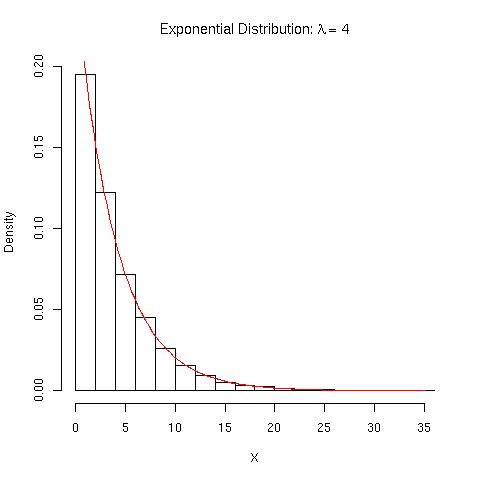
\includegraphics{expInv.jpg}    
    \caption{Sample from an Exponential(4)}
    \label{fig:expInv}
  \end{center}
\end{figure}


We can compare moments of the sample with what we expect.
\begin{verbatim}
> c(mean(x.e), var(x.e))
[1]  3.970798 15.611575
> x.s = rexp(10000, .25)
\end{verbatim}
And we can generate a sample from 
R's built-in generator and compare
the moments.
\begin{verbatim}
> c(mean(x.s), var(x.s))
[1]  3.959364 15.889116
\end{verbatim}
And these agree up to sampling error
with the values $4$ and $16$.

Of course, this simulation does not prove that the inverse CDF method
gives us a random variable with CDF $F_X(x)$.  We needed the math for
that. However, the computer does allow us to explore the technique and
get an understanding of it for particular distributions.

We use the Exponential distribution to illustrate the basics of the
Inverse CDF method. But of course we had the built-in generator
available in R so there was no need.  And, indeed, the generation
technique in R uses a different approach (given by Ahrens and Dieter).
One reason for avoiding the Inverse CDF method is that computing
$F^-1_X(u)$ may be computationally expensive relative to another
approach.  However, the Inverse CDF method is useful when the CDF is
invertible and that inverse function has a reasonably simple form and
there are no built-in functions available to us!  For example, let's
consider a random variable whose distribution is given by the
triangular distribution.  This has a density given
$$
  f_X(x) = 
  \begin{cases}%
   \frac{2(x - a)}{(b-a)(c-a)} & 0 \le x < c, \\
   \frac{2(b -x)}{(b-a)(b-c)} & c \le x \le b \\
   0 & x \not\in [a, b]    
  \end{cases}
$$
and is shown in figure \ref{fig:triangularDensity}.
\begin{figure}[htbp]
  \begin{center}
    \leavevmode
    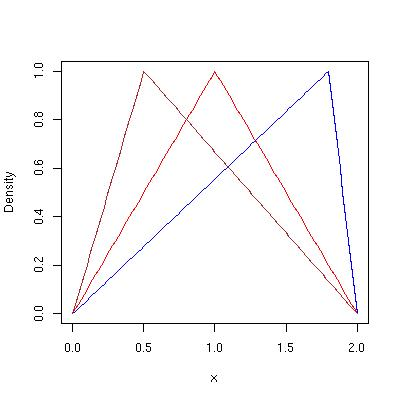
\includegraphics{triangularDensity.jpg}
    \caption{The Triangular Distribution Density.
   These are three different triangular distributions
   on the  interval $[0, 2]$
    with parameters
    $(0, 2, .5)$ (brown), $(0, 2, 1)$ (red), and $(0, 2, 1.8)$ (blue).
   }
    \label{fig:triangularDensity}
  \end{center}
\end{figure}
One can determine these formulae using
the fact that since this is a density, it 
must integrate to $1$. Since we have two triangles
and the area of a triangle is 
$1/2$ base $\times$ height, we get
\begin{eqnarray*}
 1 & = & 1/2 (c-a)\times h + 1/2 (b-c) \times h \\
 2 &=& (b-a) \times h \\
 h &=& 2/(b-a)
\end{eqnarray*}
Then, we have the two points on each line
and we can use the formula for a line.


We can integrate the two components
in the density to get the CDF.
This yields
$$
  F_X(x) = 
  \begin{cases}
  \frac{(x - a)^2}{(b-a)(c-a)} & 0 \le x < c\\
                  1 - \frac{(b -x)^2}{(b-a)(b-c)} & c \le x \le b \\
                  0 & x < 0 \\
                  1 & x > b
  \end{cases}
$$

And finally, we must compute the inverse.  Unlike the case of the
exponential distribution, we have a quadratic function here and we
have two roots.
Taking the case where $c \le x < b$, we have
\begin{eqnarray*}
  R = 1 - \frac{(b-x)^2}{(b-a)(b-c)} \\
  (1 - R)(b-a)(b-c) = (b-x)^2 \\
  \sqrt{(1 - R)(b-a)(b-c)} = b - x \\
\end{eqnarray*}
We can ignore the other root which is $-\sqrt{(1 - R)(b-a)(b-c)}$
because $b - x$ must be positive as $x \le b$ and also $R < 1$ since
it is our uniform random number.  We can similarly invert the other
term in the CDF.  All that is left is that we need to determine the
intervals for which these two pieces in the inverse CDF apply.  The
splitting point on the X axis is $c$.  However, we need this on the
uniform - $[0,1]$ - scale.  The breakpoint on this scale is the
probability or area under the CDF up to the point $c$.
In other words, it is the area of the left triangle in 
the distribution. And this is
$1/2 (c-a) h$  = $(c-a)/(b-a)$. So the 
inverse of the CDF is 
$$
  F^{-1}_X(x) =
  \begin{cases}
    \sqrt{x(b-a)(c-a)} + a &  0 \le x < (c-a)/(b-a)\\
    b - \sqrt{(1 - x)(b-a)(b-c)} & (c-a)/(b-a) \le x \le 1 \\
    0 & x < 0 \\
    1 & x > b
  \end{cases}
$$

And now we can generate random numbers from a Triangular
distribution with parameters $(a, b, c)$ with $(a \le c \le b)$
using the R function
\begin{verbatim}
rtriang =
function(n, a = 0, b = 2, c = 1) {

    if(!(a <= c && c <= b))
      stop("Incorrect parameters")

    x = runif(n)

    ans = rep(0, length(x))
    ans[x > b] = NA

    cutPoint = (c-a)/(b-a)
    A = (x > a & x < cutPoint)
    B = (x >= cutPoint & x <= b)

    ans[A] = sqrt(x[A]*(b-a)*(c-a)) + a
    ans[B] = b - sqrt((1-x[B])*(b-a)*(b-c)) 

    ans
}
\end{verbatim}

Now we can generate our samples and compare the
result
\begin{verbatim}
x = rtriang(10000, 0, 3, 1)
hist(x, prob = TRUE, xlab= "X", main = "Triangular(0, 3, 1)")
curve(dtriang(x, 0, 3, 1), 0, 3, add = TRUE, col = "red")
\end{verbatim}
And, of course,  we get very good agreement with 
the only difference being sampling variability.


\subsection{Distributions}
There are several common distributions that are amenable to the
Inverse CDF method.  We have seen the triangular and exponential
distributions.  The Extreme value, geometric, logistic, Pareto and
Weibull distributions can also be handled in this way.
The Extreme value distribution has density and CDF given
by
\begin{eqnarray*}
f_{\hbox{Extreme Value}}(x) &=& \frac{1}{\beta}e^\frac{x-\mu}{\beta}e^{-e^{\frac{x-\mu}{\beta}}} \\
F_{\hbox{Extreme Value}}(x) &=& 1 - e^{e^\frac{x - \mu}{\beta}}  
\end{eqnarray*}

The CDF of the Geometric is
\begin{equation}
  F_{\hbox{Geo}}(x) = 1 - (1-p)^x
\end{equation}


The CDF of the Logistic is
\begin{equation}
  F_{\hbox{Logistic}}(x) = 1 - 1/(1 + e^{(x - \mu)/b})
\end{equation}

The CDF of the Pareto is
\begin{equation}
  F_{\hbox{Pareto}}(x) = 1 - x^a
\end{equation}

And the CDF of the Weibull is
\begin{equation}
  F_{\hbox{Weibull}}(x) = 1 - e^{(x/a)^b}
\end{equation}



\section{Rejection/Acceptance Sampling}
The Inverse CDF approach works well if a) we can obtain a formula for
the inverse CDF, b) evaluating the formula for a given $u$ is not
excessively expensive.  If we have a density function $f_X(x)$ and we
cannot get the inverse of its CDF, then we are stuck.  How can we
generate random values from that density?  Jon Von Neumann, the
``father of computer architecture'', devised a procedure that allows
us to create samples from essentially arbitrary density functions,
$f_X(x)$.  The idea is quite simple and intuitive.  Let's focus on a
particular density, say the $\beta(4, 3)$.  This is
shown in figure \ref{fig:beta43}.
\begin{figure}[htbp]
  \begin{center}
    \leavevmode
    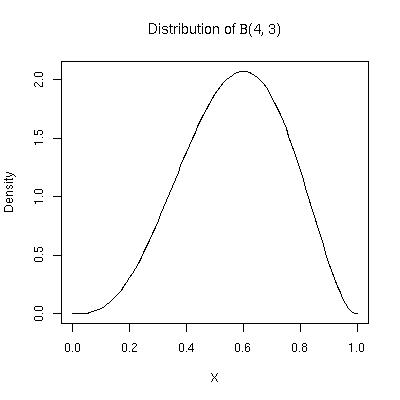
\includegraphics{beta43.jpg}
    \caption{Beta distribution - $\beta(4, 3)$}
    \label{fig:beta43}
  \end{center}
\end{figure}
What we really want to do is sample uniformly from the region under
this density.  If we could throw an infinite number of darts at the
2-dimensional plane $\Re \times \Re$ in a random way, then we could
consider only the darts that were within the region described by the
density.  Then we could take the $X$ coordinate of each of those darts
and that would constitute a random sample.  And these values would
have the appropriate density $f_X(x)$.  You should convince yourselves
that they do have the desired density.

Now, there are two problems with this approach.  We have to throw a
lot of darts!  This is time consuming and perhaps dangerous.  And if
we really throw them at random onto the entire plane, we will waste an
enormous amount of them.  Specifically, a relatively small proportion
will actually end up under the density.  After all, we are only
looking for values under the curve that ranges from $0$ to $1$ on the
X axis and from $0$ to $2.08$ on the Y axis. (\question{How can we
  determine this value?}).  What we are looking for is a more
efficient mechanism that we can use on a computer.

If we really could throw darts, we would try to narrow down the area
at which we are throwing them so that we wouldn't waste as many.
Suppose we consider the rectangle that encloses this entire density,
namely the Cartesian region $[0,1] \times [0, 2.08]$
shown in figure \ref{fig:beta43Unif}
\begin{figure}[htbp]
  \begin{center}
    \leavevmode
    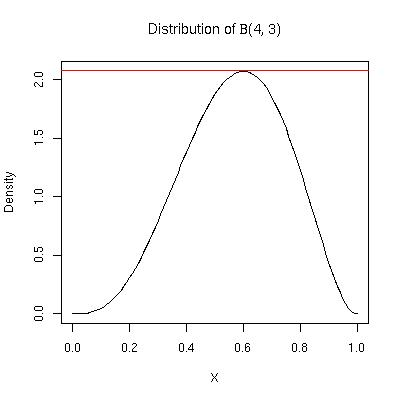
\includegraphics{beta43Unif.jpg}
    \caption{Envelope of the $\beta(4, 3)$ density.}
    \label{fig:beta43Unif}
  \end{center}
\end{figure}
If we could throw darts only in this region, then many more would be
actually ``accepted'' in our sample, i.e. be within the region under
the density.

This is the basic idea.  We try to sample uniformly from under the
density, but we cannot do this easily.  So we try to sample uniformly
from a bigger region that encloses the area of interest (our density)
and then we take only the samples within our area of interest.  If we
agree that this is a strategy that would yield a sample with the
correct distribution, i.e. with a density $f_X(x)$ then we have only
one thing left to figure out.  And that is how can we do this
practically and on a computer?

The answer involves a two-step random procedure.  We have to sample
the larger region that encloses our density.  Unlike our other random
number generation techniques, this involves sampling from a $2$
dimensional region.  So we want to avoid this if possible.  What we
will do is quite clever, thanks to John Von Neumann.  We break this
into two $1$ dimensional sampling steps.  What we do is to find a
random variable that we can sample from.  Ideally, it would have the
same \textit{support} (i.e. range) as the random variable of actual
interest (i.e the on with density $f_X(x)$).  Then, we generate a
second value that gives us the second dimension.  And this allows us
to sample uniformly in the larger region. And then we do our
``rejection-acceptance'' trick by checking whether the point is inside
the region in which we are actually interested. 

We have described this procedure in words. At some point we have to
put this into technical terms so that we can use it on the computer.
And we will also need to write it mathematically so that we can prove
that the resulting random procedure creates random values with the
correct density.  So now is a good time.  Let's suppose we can find a
second probability density function, $g_Y(y)$ that we can sample from.
Obviously, this must integrate to $1$. So its area is the same as the
density in which we are interested, $f_X(x)$.  So we know that the
density $g_Y()$ cannot entirely contain $f_X(x)$.  However, what if we
could multiply this density $g_X(x)$ by some number $c$
so that 
$$ c \times g_Y(x) \ge f_X(x) \forall x.$$ If this is possible, then
we can do the following.  Generate a random value from the density
$g_Y()$, say $y$.  Then, generate a value ($u$) from a Uniform
distribution between $0$ and $c g_Y(y)$.  We accept $y$ as being a
value in our target sample if $u < f_X(y)$.
In other words, if $u$ is within the region enclosed by $f_X(x)$,
we keep it; otherwise we reject it and return to the original
sampling steps.

So the acceptance/rejection sampling procedure in more algorithmic
terms is as follows:
\begin{enumerate}
\item Select $g_Y(y)$ and $c$ such that  
    $c g_Y(x) > f(x) \forall x$ of interest.
\item Generate a random value, $y$,  from $g_Y()$.
\item Generate a random value, $u$, from $U(0, c g_Y(y))$.
\item Accept $y$ if $u \le f_X(y)$.
  Otherwise, return to step $2$.
\end{enumerate}


Let's return to our example of the $\beta(4, 3)$.  One of the simplest
choices for $g_Y()$ is the uniform distribution.  It is especially
simple in this case as the $\beta(\cdot, \cdot)$ distribution has
support on the interval $[0, 1]$, just like $U(0, 1)$.  We then need
to select $c$ so that the density $c$ times the density $g_Y(y) = 1$
is greater than the density of the $\beta(4, 3)$.  We can eyeball this
by plotting the density $f_X(x)$ and taking a sufficiently large value
of $c$.  From figure \ref{fig:beta43Unif}, we see that anything above
$\approx 2.1$ is fine. So $2.5$ will work to be on the safe side.

What happens if we chose $c$ conservatively?  We are enlarging the
region in which we take our potential sample of values.  The larger
this is relative to the region under the density $f_X(x)$, the greater
the number of samples that will be rejected.  As a result, we will
have to generate more potential samples if we need to get a fixed
number $n$ accepted samples.  So choosing our enveloping region as
close as possible to the region of interest (i.e. under $f_X(x)$) is
highly desirable. When using the Uniform distribution, i.e. a
rectangular enveloping region, we want to chose $c$ to be the maximum
of our density $f_X(x)$.  A little calculus allows us to find this.
Alternatively, we can use R to obtain an approximate answer
by evaluating the density at different points 
\begin{verbatim}
 max(dbeta(seq(0, 1, length = 100000), 4, 3)
\end{verbatim}
yielding $2.07$.


So now we are set to perform the different steps to generate a value
from a $\beta(4, 3)$ random variable.
\begin{verbatim}
 while(TRUE) {
   y = runif(1)
   u = runif(1, max = 2.07 * y)
   if(u < dbeta(y, 4, 3))
     break
}
\end{verbatim}

I have written some functions that allow us to explore different
choices of $g_Y()$ and to generate samples.
Using a simple rectangular sampling region
via the standard Uniform density for $g_Y()$,
we get
\begin{figure}[htbp]
  \begin{center}
    \leavevmode
    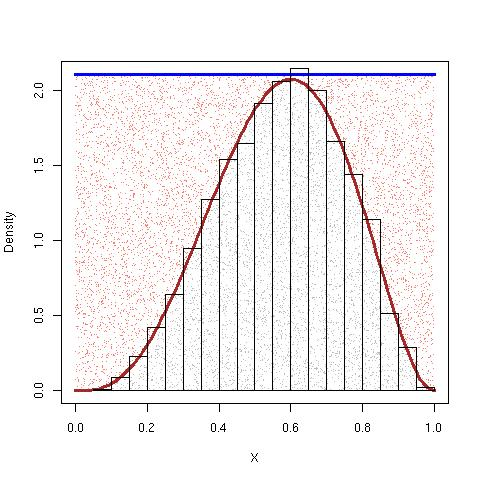
\includegraphics{ARSBetaUnif.jpg}
    \caption{Acceptance/Rejection using the triangular distribution}
    \label{fig:betaUnif.jpg}
  \end{center}
\end{figure}
The proportion of samples that were accepted is $47.3\%$.
We see that the sample histogram is very close to the
density and the variation is just sampling error.

By choosing a better enveloping region, we can improve the acceptance
rate.  In the case of the $\beta(4,3)$ density, we can use a
triangular distribution as $g_Y()$ and scale it to create an envelope
region. The particular choice of triangular distribution is $Tr(0, 1,
.8)$ and we choose $c$ to be $1.6$.  The plot in figure
\ref{fig:betaTriang.jpg} shows this region.
\begin{verbatim}
acc = ars.eg(function(x) dbeta(x, 4,3), 
             function(x) dtriang(x, 0, 1, .8), 
             1.6, 
             function(n) tr.inv(runif(n), 0, 1, .8), 
             10000)
\end{verbatim}
\begin{figure}[htbp]
  \begin{center}
    \leavevmode
    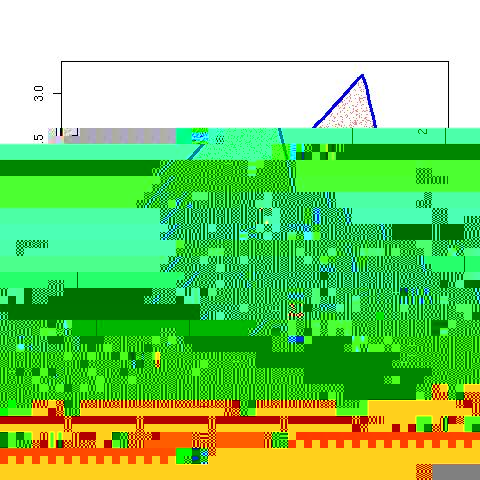
\includegraphics{ARSBetaTriangular.jpg}
    \caption{Acceptance/Rejection using the triangular distribution}
    \label{fig:betaTriang.jpg}
  \end{center}
\end{figure}
The acceptance rate for this is $62\%$.


\section{Markov Chain Monte Carlo - MCMC}
In most simulation contexts, we are interested in estimating the
expression $E_{f_X}[g(X)]$.
If we have i.i.d. samples from the random variable with density $f_X$
of the form $x_1, \ldots, x_n$, we can estimate this value
as
\begin{equation}\label{egx}
 E_{f_X}[g(X)] \approx \frac{1}{n} \Sigma_{i=1}^n g(x_i)
\end{equation}
The law of large numbers tells us that this is a good estimator.
Using different functions $g()$, we can obtain estimates for different
properties.  For example, $g(x) = x$ gives us the expectation of the
random variable.


Identical and independent values may be hard to sample from $f_X(x)$.
But we can use the estimator above in \ref{egx} if the $x_i$ are not
independent but sampled from $f_X(x)$ in proportion to $f_X()$.  The
computation of the variance is more complicated in these
circumstances, but the estimator is good.  This is because
\begin{equation}
  E_{f_X}[g(x)] = \int g(x) f_X(x) dx
\end{equation}
So if we can generate $x_i$ from $f_X()$ we can use Monte Carlo to
solve many problems.

The problem that we are now faced with is how to generate sample
values from the density $f_X(x)$, dependent or independent.  It turns
out that this is actually quite simple if we use what are called
Markov Chains.  Consider the following technique for generating a
sequence of random values.  Define $X_{t+1}$ by sampling from a
distribution that only depends on $X_t$, i.e. the current state of the
sequence.  In other words, we have a probability distribution given in
general terms as $P(X_{t+1} \vert X_t)$.  This sequence ${X_t}$ is
called a Markov chain.

To get the sequence started, we need a starting value $X_0$.  But
$X_{t}$ will depend on the value of $X_0$.  For many probability
distributions $P(X_{t+1} | X_t)$, it turns out that $P(. | X_0)$ is
independent of $X_0$ and it doesn't matter where we start.  And under
certain conditions, the sequence ${X_t}$ converges to a stationary
distribution, $\pi(x)$, which does not depend on $t$ or $X_0$.  Thus
for a sufficiently large value of $t$, $t_0$, $X_{t_{0} + 1}, X_{t_{0}
  + 2}, \ldots$ are samples (\textit{not} necessarily independent)
from the density $\pi(x)$.
So we can estimate $E_{g_X}[X]$ as 
\begin{equation}
  \frac{1}{n - t_0}\Sigma_{i = t_0}^n g(x_i)
\end{equation}


All that remains to use this technique is to create the Markov Chain.
In other words, we must specify the value $P(X_{t+1} \vert X_t)$ so
that we obtain the desired stationary distribution $f_X(x)$.  This
seems like a hard task, but it turns out to be quite simple.  Suppose
we have a distribution function $q(\cdot \vert X_t)$ which we will
call our \textit{proposal} distribution.  For a given $t$, we generate
a sample from a random variable $Y$ with this density.  We call $q()$
a proposal distribution because we don't use it directly to generate
$X_{t+1}$ in our sequence. Instead, we generate this new value but,
like acceptance/rejection sampling, we decide whether to accept it
under certain conditions.  Specifically, we use an decision algorithm
to accept or reject this new value.
The Hastings algorithm decides to accept this new value
with probability
$$
 min(1, \frac{f_X(Y)}{f_X(X_t)})
 $$ In other words, we toss a weighted coin with probability $ min(1,
 \frac{f_X(Y)}{f_X(X_t)})$ and if it turns up heads, we accept the new
 value $Y$ as the next step in the sequence, $X_{t+1}$.  If the coin
 ends up tails, we stay where we are and $X_{t+1} = X_t$.  This
 acceptance probability essentially favors $Y$ if $Y$ is more likely
 than the current value $X_{t}$.

The Metropolis-Hastings algorithm adds a variation to this.
Instead of looking at the likelihood ratio of $f_X(Y)/f_X(X_t)$,
it uses
$$
 \frac{q(X\vert Y) f_X(Y)}{q(Y\vert X) f_X(X)}
 $$ 
where $q$ is our proposal distribution again.
This yields nice properties that allow the Markov Chain to be
reversible and generally nicely behaved.

Regardless of which algorithm we use to accept or reject or our
proposal $Y$, the algorithm for generating the steps in the Markov
Chain are quite simple.

We need a function to generate a value from our proposal distribution.
This is the argument \SArg{r}.  To compute the acceptance probability,
we need $f_X()$, the stationary target density.  And if we are using
the Metropolis-Hastings algorithm we also need the density of the
proposal distribution given by \SArg{q}.  And we need a starting
point, $X_0$.  \SArg{n} says how many elements in the sequence we
should generate.  We need this to be large enough so that the chain
converges to $f_X()$ and yields sufficient sample values.
\begin{verbatim}
mcmc =
function(x.0 = 0, r, q, stationary, n = 1000, algorithm = metropolis)
{
     xs = numeric(n+1)  # space for the answers
     xs[1] = x.0
     for(i in 1:n) {
       y = r(xs[i])   # Generate proposal
       k = algorithm(xs[i], y, stationary, q)
       xs[i+1] = ifelse(runif(1) <= k, y, xs[i])
       if(is.na(xs[i+1])) {
        stop("Problems in MCMC")
       }
     }

     class(xs) <- "mcmc"
     xs
}
\end{verbatim}

Let's generate a sample from a t-distribution with $10$ degrees of
freedom, $t(10)$.  This is the stationary distribution that is our
target.  We can use the R function \SFunction{dt} to compute the
density.  We will use a Normal distribution as our proposal
distribution with mean $X_t$ and variance $1$.  We can use
\SFunction{rnorm} to generate proposal values and \SFunction{dnorm} to
calculate the density in the Hastings algorithm.
We'll generate $10,000$ values and then look at the last
$5000$ to give this adequate time to ``burn in'' or converge
to $t(10)$. We'll chose a strange starting value of $-10$
to illustrate how this converges.
\begin{verbatim}
 xt = mcmc(-10, 
           r = function(x) rnorm(1, x), 
           q = function(x, y) dnorm(y, x), 
           stationary = function(x) dt(x, 10), 
           alg = hastings, 
           n = 10000)
\end{verbatim}
We can see how well the sample approximates the
true density $t(10)$ in figure
\begin{figure}[htbp]
  \begin{center}
    \leavevmode
    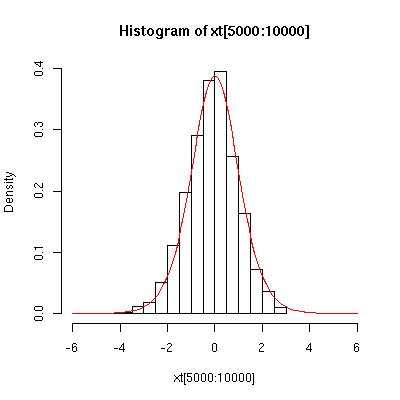
\includegraphics{mcmcT10.jpg}
    \caption{MCMC sample from $t(10)$.}
    \label{fig:mcmcT10.jpg}
  \end{center}
\end{figure}
This looks pretty close and within sampling variation.


The MCMC  approach to estimating $E[g(X)]$ and sampling dependent
values from a density is very powerful and is similar in ways to the
acceptance/rejection sampling we covered above.  One does have to
honor the conditions on the proposal and stationary distributions to
ensure that the Markov chain converges and converges to $f_X()$.


\end{document}


\setcounter{chapter}{6}
\def\charClass#1{[[:#1:]]}
\def\code#1{\texttt{#1}}
%\chapter{Regular Expressions}
\chapter{Text Data and Regular Expressions}
\section{Introduction}
Although binary files allow us to explicitly encode the type of a value, 
be it an integer, real number, string, etc., much of the
data we deal with are given to us as plain text.  We input numbers in text
files, download text files from Web and FTP servers, and save
spreadsheets as comma-separated values in .csv files. 
%numbers into tables to be transferred in regular text files.
%Genomic sequence data are long strings from the 4 letter alphabet \{A,
%C, G, T\}.  
In these cases, the data are merely represented by their
text form and are easily interpreted by applications.  However, there
are many examples of more complex situations where the data are not as
easily interpreted, and  the text must be processed to
create the values of interest.  A simple example of this phenomenon is
when numeric values are embedded into text, but not in a regular or
simple format, such as numbers in an HTML table.  
In this case, we must extract the elements of interest from
the text content by identifying the patterns where the values occur.  
A different sort of example occurs when text itself makes up the data, 
such as a speech, an abstract, or an email message.  Then we must search
for the presence of certain words or phrases in particular contexts or places
to uncover structure in the data, e.g. we
might examine how often each word is used, the names of the author(s), 
the use of punctuation, etc.
Finally, documents and text are sometimes treated directly as
data such as in search engines, databases, and so on.   


\subsection{Placing data on a map}\label{ssec:map}

To make a county map of the United States (Figure~\ref{fig:countyMap}
in Chapter~\ref{chap:Maps}) that displays election results, and
possibly census data too, requires the various sources of information
to be merged together. This merger uses county name, a text field,
which needs to be \textit{transformed} into a uniform format across
the three sources.  The following sample lines of text demonstrate the
inconsistencies in how a county's name is represented in these three
sources of data; geographic (top), census (middle) and election
(bottom).  Notice that there is no period after \verb+''St''+ in the
geographic data; the election results differ from the other two
sources in that there is an \verb+&+ rather than ``and'' in Lewis and
Clark County; the capitalization is not consistent (e.g. ``Qui'' vs
``qui'' in Lac qui Parle County); and the use of ``County'' and
``Parish'' is not consistent.
\begin{comment}
Unfortunately the naming conventions for the counties are slightly
different from one source to the next.  For example, the county names
in the election data do not contain ``County'' as part of the name but
the other sources do include it in the name.  Also, the county names
in the geographic data do not include the period after ``St.'' in
names such as St. John the Baptist, but the other sources do use the
period.  In order to match up the election results with the census
data and plot them in the proper place these inconsistencies must be
resolved.
\end{comment}

{\footnotesize{
\begin{verbatim}
"De Witt County",IL,40169623,-88904690
"Lac qui Parle County",MN,45000955,-96175301
"Lewis and Clark County",MT,47113693,-112377040
"St John the Baptist Parish",LA,30118238,-90501892

"St. John the Baptist Parish","43,044","52.6","44.8",...
"De Witt County","16,798","97.8","0.5", ...
"Lac qui Parle County","8,067","98.8","0.2", ...
"Lewis and Clark County","55,716","95.2","0.2", ...

DeWitt  23      23      4,920   2,836   0
Lac Qui Parle   31      31      2,093   2,390   36
Lewis & Clark   54      54      16,432  12,655  386
St. John the Baptist    35      35      9,039   10,305  74
\end{verbatim}
}}
\begin{comment}
  \caption{These sample lines of text demonstrate the inconsistencies
    in how a county's name is represented in three sources of data:
    geographic (top), census (middle) and election (bottom).  Notice
    that there is no period after ``St'' in the geographic data; the
    election results differ from the other two sources in that there
    is an ``\&'' rather than ``and'' in Lewis and Clark County; the
    capitalization is not consistent (e.g. ``Qui'' vs ``qui'' in Lac
    qui Parle County); and the use of ``County'' and ``Parish'' is not
    consistent.}\label{fig:censusRegEx}
\end{comment}


\subsection{Spam filtering}\label{ssec:spam}
In Chapter~\ref{chap:spam} we explore the problem of filtering email
to try to differentiate legitimate electronic mail from unsolicited
bulk email, i.e. spam.  One approach considered \textit{creates}
several variables pertaining to the email message and then uses the
values of these variables for a mail message to predict whether it is
spam or not.  A potentially useful variable is one that indicates
whether the subject line of the email message contains a ``word'' with
punctuation or a digit in the middle of it, such as ``V!agra'' or
``m0rtgage''.  

Below are parts of the header from three email messages.  The bottom
two headers are from spam while the top is not. 
{\footnotesize{
\begin{verbatim}
Date: Tue, 02 Jan 2007 12:17:45 -0800
From: Duncan Temple Lang <duncan@wald.ucdavis.edu>
To: Deborah Nolan <nolan@stat.Berkeley.EDU>
Subject: Re: 90 days

Date: Sat, 27 Jan 2007 16:28:48 +0800
From: remade SSE <glzmeqrxr99@embarqhsd.net>
To: depchairs03-04@uclink.berkeley.edu
Subject: [SPAM:XXXXXXXXX]

Date: Thu, 03 Apr 2008 09:24:53 +0700
From: Faustino Britt <Faustino@sfera.umk.pl>
To: Brice Frederick <nolan@stat.Berkeley.EDU>
Subject: Fancy rep1!c@ted watches
\end{verbatim}
}}
Notice that the last subject line contains the ``word''
\verb+rep1!c@ted+ rather than ``replicated''.  These fake words are
popular in spam because they are easy for us to read, but they are not
likely to be found in a list of ``banned'' words, i.e. words that a
spammer would use.  Another variable that may be helpful in detecting
spam is a logical that indicates whether or not the subject line of an
email message begins with ``Re:'' Yet another is whether or not the
reply-to address contains an underscore or digit.


\subsection{Weblogs}\label{ssec:weblog}
To analyze the requests made to a Web site, we first \textit{extract}
the relevant information from the Web log, such as the machine of
requester, the time and date of the request, the name of the file
requested, the return status, and the number of bytes returned.  Below
are two lines from a Web log.  The log is a text file where each
request appears on a separate line of text, and although the text has
a lot of structure, the information does not appear in a simple format
such as in comma separated values, nor is it placed consistently in
the same columns in the file. For example, the date and time are set
off in square brackets.  Note that each line in the Web log is broken
across four lines here for formatting purposes.  {\footnotesize{
\begin{verbatim}
169.237.46.168 - - [26/Jan/2004:10:47:58 -0800] 
  "GET /stat141/Winter04 HTTP/1.1" 301 328 
  "http://anson.ucdavis.edu/courses/" 
  "Mozilla/4.0 (compatible; MSIE 6.0; Windows NT 5.0; .NET CLR 1.1.4322)"
169.237.46.168 - - [26/Jan/2004:10:47:58 -0800] 
  "GET /stat141/Winter04/ HTTP/1.1" 200 2585 
  "http://anson.ucdavis.edu/courses/" 
  "Mozilla/4.0 (compatible; MSIE 6.0; Windows NT 5.0; .NET CLR 1.1.4322)"
\end{verbatim}
}}

 
\subsection{Mining the State of the Union addresses}\label{ssec:sou}
We \textit{mine} the text of the State of the Union Addresses, looking
for similarities between presidents' speeches.  One approach to doing
this would be to compare word frequencies across documents in the
corpus of speeches.  To do this, we build a word-vector for each
speech that tallies the number of occurrences of each word used in the
speech, e.g. there was one occurrence of the word ``much'', the word
``debt'' was used twice, and the words ``nation'', ``national'' or
``nations'' appeared five times in the December, 1790 inaugural speech
of George Washington's (a snippet is shown below).  With these
word-vectors we can look for similarities between the distribution of
words in the speeches.  to create the word-vector, we first stem words
(i.e. reduce ``running'' to ``run'') and remove stop words such as
``and', ``the'', and ``of''.  {\footnotesize{
\begin{verbatim}
***

State of the Union Address
George Washington
December 8, 1790

Fellow-Citizens of the Senate and House of Representatives:

In meeting you again I feel much satisfaction in being able 
to repeat my congratulations on the favorable prospects which
continue to distinguish our public affairs. The abundant fruits
of another year have blessed our country with plenty and with 
the means of a flourishing commerce.
\end{verbatim}
}}


The regular expression language is essentially a programming language,
and with it we can develop complicated constructs, making use of the
rich set of meta characters that it employs, to analyze each of these
data sets.  The goal of this chapter is to demonstrate the fundamental
ideas behind the language, to introduce the basic elements in the
language, and show how they can be combined to express patterns.
There are many tutorials and examples on the Web that cover different
uses and applications of regular expressions.  There are also books on
the subject that provide many more examples and a greater
understanding of how regular expressions work.  Most important of all,
practice in creating regular expressions and testing them on data is
essential to gaining both understanding and experience so that when
you need to use regular expressions in handling data, they will be
familiar.


\begin{figure}
\begin{center}
\textbf{Examples of Uses of Regular Expressions on Text Data}
\end{center}
\begin{itemize}
\item EXTRACT pieces of text that appear in non-standard formats.

\item CREATE variables from information found in text.

\item CLEAN and TRANSFORM text into a uniform format and resolve inconsistencies in format between files. 

\item MINE text by treating documents directly as data.

\end{itemize}
\end{figure}


\section{Matching literal strings}

The inconsistencies in the various sources of information for making
the election map (Section~\ref{ssec:map}) are easily remedied.  For
example, ``County'' or ``Parish'' can be removed from the end of each
county name.  Fixing the problem with the missing period in the names
such as ``St John the Baptist Parish'' is slightly more subtle.  Many
counties in the United States have ``St'' in their names and we want
to make sure that we change all occurrences of ``St'' to ``St.''
However, we also want to be sure not to change, a name such as,
``Stone County'' to ``St.one County''.  If we search for the pattern
\verb+'St '+ and change it to \verb+'St. '+, then that should avoid
this problem.
 
Rather than edit data files manually, it is better to make the changes
programmatically in order to keep a record of the changes required in
case mistakes are made or the process needs to be repeated when the
data change.  Using any general programming language such as Matlab,
Java, C, Perl, etc., we could develop a function to perform this
simple task for operating on strings and patterns within them.
{\footnotesize{
\begin{verbatim}
> string
[1] "St John the Baptist Parish"
> if ("St " == substring(string, 1, 3))
+     newString = paste("St. ",             
+            substring(string, 4, nchar(string)), sep ="")
> newString
[1] "St. John the Baptist Parish"
\end{verbatim}
}}

If we are not sure that the pattern will occur at the beginning of the
string, then we need a more general approach.  Below we split the
input string into a vector of single characters, and iterate over
these characters looking for the particular string.  That is,
determine which of these characters are possible starting points of
the pattern, i.e. \verb+S+.  
{\footnotesize{
\begin{verbatim}
> characters = unlist(strsplit(string, "") )
> characters
 [1] "S" "t" " " "J" "o" "h" "n" " " "t" "h" 
[11] "e" " " "B" "a" "p" "t" "i" "s" "t" " "
[21] "P" "a" "r" "i" "s" "h"
> possible = which(characters == "S")
> substring(string, possible[1], possible[1] + 2)
[1] "St "
\end{verbatim}
}}

\subsection{Fundamental Approach}
We can write a more general R function that would determine if an input text
\SVariable{string}
contained the argument \SVariable{pattern}.
{\footnotesize{
\begin{verbatim}
findPattern = function(pattern, string) {
  lets = strsplit(string,"")   
  firstLetter  = substring(pattern, 1, 1)
  possibles = which(lets[[1]] == firstLetter)
  if (length(possibles) > 0)
       any(pattern == substring(string, possibles, 
             possibles + nchar(pattern) -1))
  else return(FALSE)
}
\end{verbatim}
}}
\noindent 
This function matches a \textit{literal} string given by
\SVariable{pattern} within the given \SVariable{string} by searching
for all the occurrences of the first character in \SVariable{pattern}
and then looking at all substrings with the same length as
\SVariable{pattern} starting from those points.  It illustrates the
fundamental approach to pattern matching, e.g. when we look for the
literal string \verb+St + in a line of text.  When we write down a
regular expression pattern like \verb+'St '+, what is meant is really
the following: find the character \verb+S+ immediately (i.e. the next
character) followed by \verb+t+, immediately followed by a blank
character.  What the regular expression matching engine does is, for
the target string, start at the first character and check to see if it
is an \verb+S+. If not, then move to the second character and start looking
there.  When it finds an \verb+S+, it then checks if the next character is
a \verb+t+. If not a \verb+t+, then start over and check if this character is
an \verb+S+ and so on.  So we can think of the literal string as being made
up of three consecutive sub-patterns: \verb+S+, \verb+t+ and ` '.  Thinking of
the pattern \verb+'St '+ in this way makes it easier to see how to combine
different types of complex patterns to define a sequence (see
Figure~\ref{fig:literalString} for an example of this search process).


\begin{figure}
{\footnotesize{
\begin{verbatim}
           The Slippery St Frances.
               ||       |||
               ||       |||
Found S _______||       |||
Followed by t?__| No    |||
Is it S? _______| No ...||| Keep looking for an S
                        |||
Found S ________________|||
Followed by t? __________|| Yes
Followed by blank? _______| Yes  - A Match!
\end{verbatim}
}}
\caption{A diagram of a search for the literal string `St '.  The
  regular expression matching engine looks for the first character
  `S', immediately followed by t', immediately followed by blank.
  When it finds the `S' in Slippery, it then checks if the next
  character is a `t'. Since it is not, it starts over and checks to
  see if it is an `S', and continues looking for an `S'.  The most
  basic building block in a language that supports matching patterns
  in text is a facility for specifying a short string of text in a
  literal string as a pattern to match.}\label{fig:literalString}
\end{figure}

There are two functions in R, \SFunction{gsub} and \SFunction{sub},
that look for the pattern and replace it within a string with some
other text.  Each of these functions takes three arguments: the
regular expression (pattern) defining what to match, another regular
expression to use as the replacement text, and the string(s) on which
to do the matching and substitution.

The `g' in the name \SFunction{gsub} refers to \textit{global}.  This
means that it changes all the matches of the regular expression in the
text with the replacement pattern.  The \SFunction{sub} is almost
exactly the same as \SFunction{gsub} except that it only replaces the
first occurrence of the pattern with the replacement text.  In our
example here, we expect there to be one occurrence of ``St '' in the
string, and so \SFunction{sub} should work fine.  {\footnotesize{
\begin{verbatim}
> countyNames
[1] "Dewitt County"              "Lac qui Parle County"      
[3] "St John the Baptist Parish" "Stone County"              
> gsub("St ", "St. ", countyNames)
[1] "Dewitt County"               "Lac qui Parle County"       
[3] "St. John the Baptist Parish" "Stone County"   
\end{verbatim}
}}

As an illustration of how \SFunction{gsub} differs from
\SFunction{sub}, we replace the word (or literal string, actually)
``one'' with the digit ``1'' in the following simple character vector.
{\footnotesize{
\begin{verbatim}
> strings =  c("a test", "and one and one is two", 
        "one two three")
> gsub("one", "1",strings)
[1] "a test"  "and 1 and 1 is two"  "1 two three"       
\end{verbatim}
}}
\noindent 
Notice, there was no ``one'' in the first string (``a test''), so there was no way to substitute the match with the replacement text (``1'').  So it remains unaltered and is returned as is.  In the second string, there are two occurrences of the string ``one''.  Each of these are replaced with the digit ``1''.  And similarly, the third string has its single occurrence of ``one'' replaced with ``1''.  In contrast, the \SFunction{sub} replaces only the first occurrence of
    ``one'' with ``1'' in the second string.  
    {\footnotesize{
\begin{verbatim}
> sub("one", "1", strings)
[1] "a test"   "and 1 and one is two"  "1 two three"         
\end{verbatim}
}}

The language of regular expressions is far more powerful than
illustrated by this simple example.  The next examples build on this
pattern matching technique to demonstrate the more advanced features
of the regular expression language.


\section{Character Classes}

Searching the subject line for ``Re:'' in an email message
(Section~\ref{ssec:spam}) is a task similar to the pattern search in
the previous example; the simple function \SFunction{findPattern} should
easily handle the job.  The other patterns present more of a
challenge.  For example, if we are looking for email addresses that
contain digits, then any digit $0$ through $9$ found anywhere in the
address would be considered a match.  The function
\SFunction{findPattern} cannot handle this more complicated pattern, as
it is only capable of performing a simple literal string comparison.
Here we want to ask about alternative patterns, i.e. of the form this
or that. In this case, we could split the string into separate
characters and check whether any of these are digits.  Similarly, to
find a fake word that contains punctuation in the middle of it, we
could split the subject line into individual characters, search for
punctuation or a digit, and if we find it, then look at the preceding
character and the succeeding character to ascertain whether they are
letters of the alphabet (upper or lower case).  So any
letter--punctuation or digit--letter combination is a match.

We can write a suite of functions to perform the different types of
matching and substitutions required of this problem. Since the search
for any digit or any alpha character are commonly needed, it is
reasonable to guess that others might have already implemented these
for their purposes and we might be able to reuse their code.  As with
all software, we would like to reuse such code as it is likely to be
better tested and more efficient than our initial efforts.  Ideally,
we would be able to use a language to express these patterns in a
unified manner. Indeed, the regular expression language is such a
general language that has several implementations that are well-tested
and efficient.

It provides basic building blocks for specifying patterns that are to
be matched in a piece of text.  These allow us to match literal
strings, a character from a particular set of characters or its
complement (character sets), and one sub-pattern or another
(alternation).  We can also match by position such as at the beginning
or end of a line, and we can create sub-patterns from individual
patterns by specifying the number of times the pattern should be
matched (quantifiers).


\subsection{Equivalent Characters}\label{sec:charClass}
For the search in an email address for a digit, the pattern we want to
match could contain any digit: 0, 1, 2, 3, 4, 5, 6, 7, 8 or 9.
Regular expressions allow us to succinctly express the concept of
``match a digit'', by explicitly enumerating the equivalent
characters.  We use the \verb+[ ]+ notation to identify a collection of
equivalent characters, called a \textit{character class}, that specify
the collection of characters that constitute a match.  For example, to
match a digit, we us \verb+[0123456789]+.  Similarly to match a lower
case letter, we use 
{\footnotesize{
\begin{verbatim}
[abcdefghijklmnopqrstuvwxyz]
\end{verbatim}
}}
\noindent
and to match a space or a TAB character, we use
\verb+[ \t]+.

Basically, we can enumerate any collection of characters within the
$[$ $]$ and these are included in the set of characters that
constitutes a match. We also adapt this notation very slightly to
indicate a match on the complement of the set of characters.  That is,
we place a caret $\wedge$ as the first character within \verb+[]+
to indicate that the equivalent characters are the complement of the
characters enumerated within, i.e. anything but these characters is
considered a match.

There are many collections of characters that are commonly used. For
example, we often want to specify all the letters of the alphabet,
lower or upper case or both. And we often want all the digits.  And in
other cases, we want a subset of these sets.  The $-$ character when
used within the character class pattern (i.e. the \verb+[]+) typically
identifies a range.  We can specify the digits $0$ through $9$ more
readily as \verb+[0-9]+ and the subset of the digits $3$, $4$, $5$,
$6$ can be specified as \verb+[3-6]+.  Similarly, we can specify
\verb+[0-9A-F]+ to match all the hexadecimal digits.  And you will
often see \verb+[A-Za-z]+ for all letters (upper and lower case) in
the alphabet.  Once again, the pattern expresses a higher level
concept that is easier to read than explicitly enumerating the
elements of the character set.

Note, if we want to include the character $-$ in our set of characters
to match, then we must put this at the beginning of the character set,
otherwise it is interpreted as a range.  For example, to match the
basic arithmetic operators $+$, $-$, $*$ or $/$, we can use
\verb%[-+*/]%
Or to match a digit with either a $+$ or $-$ in front of it, we can
use \verb%[-+][0-9]%
That is, we have made an overall pattern from a \textit{sequence} of
two sub-patterns and each of these sub-patterns is made up using the
primitive elements.  The first \verb+-+ is for the literal character
and the second is for the special character that denotes a range.

\subsection{Named Character Classes}
Character classes are very convenient, and the range operator ($-$)
succinctly specifies collections of characters to further simplify
their use.  The regular expression language also provides a collection
of built-in character sets for commonly used collections.  Each of
these is identified by a short name.  See
Table~\ref{table:charClasses} for a description of some of these named
character sets.

\begin{table}
\begin{center}
\begin{tabular}{ll}
Name & Collection of characters \\
\hline
\charClass{alnum} & All alphabetic and numeric \\
\charClass{alpha} & All alphabetic \\
\charClass{lower} & Lower case alphabetic characters \\
\charClass{upper} & Upper case alphabetic characters \\
\charClass{digit} & Digits $0 1 2 3 4 5 6 7 8 9$\\
\charClass{punct} & Punctuation characters \\
\charClass{blank} & Blank characters, i.e. space or tab \\
\charClass{space} & White space \\
\charClass{cntrl} & Control characters, e.g. new line  \\
\charClass{print} & Printable characters \\
\charClass{graph} & Printable character except space \\
\end{tabular}
\end{center}
\caption{Some useful named character classes.}\label{table:charClasses}
\end{table}

We use these collections with the same \verb+[]+ notation, but we
specify the named character set with an additional \verb+[::]+ pair.
So, for example, to specify the punctuation characters, use
\verb+[[:punct:]]+ The \verb+[:punct:]+ term is the named character
class.  Additional characters can be included in the overall set such
as \verb+[[:digit:]_]+ to consider a match any digit \textit{or} the
\_\_ underscore character.

The search for a digit or an underscore in the email can now be easily
performed.  
{\footnotesize{
\begin{verbatim}
> Addresses
[1] "Duncan Temple Lang <duncan@wald.ucdavis.edu>"
[2] "depchairs03-04@uclink.berkeley.edu"  
[3] "Faustino Britt <Faustino@sfera.umk.pl>"        
> grep("[[:digit:]_]", Addresses)
[1] 2
\end{verbatim} 
}}
\noindent 
The \SFunction{grep} function in R takes two arguments, the
regular expression specifying the overall pattern to match and then a
character vector containing the different text strings on which to
search.  It returns the indices of the elements of that character
vector for which there was a match (or the empty integer vector if
none matched).  This can be readily used to subset the character
vector to get only the elements containing or not containing that
pattern.  The return value from the call to \SFunction{grep} above is
$2$ because a digit was found in the second element of the character
vector \SVariable{Addresses}. The \SFunction{grep} is also available
in the shell (see Chapter~\ref{chap:shells}).

The search for a fake word that contains punctuation or a digit in the
middle of it is handled by the following pattern 
{\footnotesize{
\begin{verbatim}
[[:alpha:]][[:digit:][:punct:]][[:alpha:]]
\end{verbatim}
}}
\noindent 
Paying careful attention to the square brackets in this pattern,
we see that we are looking for three characters.  The first can be any
letter in the alphabet (upper or lower case), followed by a digit or
punctuation mark, followed by another letter.  Unfortunately this pattern
matches the text string ``it's'', which we do not want.  This problem can be
resolved by providing the specific punctuation marks that are
acceptable in the character class, 
{\footnotesize{
\begin{verbatim}
[[:alpha:]][[:digit:]!@#$%^&*():;?,.][[:alpha:]]
\end{verbatim} 
}}
\noindent 
or we could first remove any quotation marks from the search
string and then use the original pattern.  
{\footnotesize{
\begin{verbatim}
> s = c(subjectLines, "It's me")
> s
[1] " Re: 90 days"     "[SPAM:XXXXXXXXX]"         
[3] " Fancy rep1!c@ted watches"  "It's me" 
> newString = gsub("'", "", s)
> grep("[[:alpha:]][[:digit:][:punct:]][[:alpha:]]", newString)
[1] 2 3
\end{verbatim}
}}
\noindent 
Note that the search did not match the ``Re:'' because the colon
is followed by a blank, nor does it match the fourth element because
the \verb+'+ has been removed from the string.  It does find a match
in the second element and the third element.  To find exactly where the pattern was found in these strings, we can use the \SFunction{regexpr} function.
{\footnotesize{
\begin{verbatim}
> regexpr("[[:alpha:]][[:digit:][:punct:]][[:alpha:]]",
       newString)
[1] -1  5 13 -1
attr(,"match.length")
[1] -1  3  3 -1
\end{verbatim}
}}
\noindent
The return value of $-1$ indicates that the pattern was not found in the first and fourth elements of \SVar{newString}.  As for the second element, the return value of $5$ indicates that the pattern was found beginning at the fifth character in the string, and the value of the attribute \SVar{match.length} for this element in the return vector indicates that the match is three characters long.  The fifth through eighth characters in \verb+[SPAM:XXXXXXXXX]+ are  \verb+M:X+ and so we have found the pattern we expected to find. 

Notice that the match found in the  third element of \SVar{newString} uncovers one more limitation in our pattern specification: the pattern was found in characters 13-15 in the string, i.e. \verb+c@t+.  That is,
we did not find \verb+p1!c+ because it consists of four characters: a letter, followed by a digit,
followed by a punctuation mark, followed by a letter.  To search for the more general pattern of any number of digits or punctuation marks between letters, we must change the pattern as follows.
\begin{verbatim}
[[:alpha:]][[:digit:][:punct:]]+[[:alpha:]]
\end{verbatim} 
The plus sign between the second and third characters in the pattern indicates that 
the second character may appear one or more times.


\subsection{Meta Characters}
The characters \verb+[ ]+ and \verb+[: :]+ and \verb%+% are given special meaning
  in a pattern; these special characters are called meta
  characters. Regular expressions offer a rich set of meta characters
  for pattern matching.  For example, meta characters make easy work
  of the task to derive is a logical that indicates whether or not the
  subject line in an email is all capital letters.  This phenomena in
  email is referred to as yelling.  Here is a case when the complement
  of a character set is useful because we allow any character except
  lower case letters of the alphabet in the subject line of the email.
  But we face the problem of needing every character in the subject
  line to \textit{not} be a lower case letter.  We want to specify a
  pattern that consists of non-lower case letters from the beginning
  to end without knowing how long it is.  Again, we can write a
  specialized function to do the work, 
 {\footnotesize{
\begin{verbatim}
> subjectLines
[1] " Re: 90 days"      "[SPAM:XXXXXXXXX]"         
[3] " Fancy rep1!c@ted watches"
> all(strsplit(subjectLines,"")[[1]] %in% LETTERS)
> FALSE
\end{verbatim}
}}
\noindent 
but regular expressions provide a clean, clear way to express
this pattern via meta characters.  
{\footnotesize{
\begin{verbatim}
^[^[:lower:]]*$+
\end{verbatim}
}}
\noindent 
To explain, the first character in this pattern, the \verb+^+
    is the anchor for the beginning of the string, and the last
    character, \verb+$+ is the anchor to specify the end of a string.
    The asterisk denotes ``any number of times'' meaning that the
    character immediately preceding it may be repeated zero or more
    times.  Put all together, the pattern finds a match when the string
    consists entirely of non-lower case letters from beginning to end.
    Note that the caret \verb+^+ appears twice in the pattern, and each
    occurrence has a different meaning.  The first caret is the meta
    character for the beginning of line anchor, and the second caret,
    which is the first character inside the square brackets, represents
    the complement meta character that says any character that is not a
    lower case is a match.  
{\footnotesize{
\begin{verbatim}
> grep("^[^[:lower:]]*$", subjectLines)
[1] 2
\end{verbatim}
}}


\begin{table}
\begin{center}
\begin{tabular}{lp{4in}}
Character & Meaning \\
\hline
\verb+^+ & As the first character in the pattern, anchor for beginning of line\\
         & As the first character inside $[$ $]$, exclude these characters.\\
\verb+$+ & End of line anchor \\
\verb+?+ & Character or sub-pattern occurs zero or one time\\
\verb%+% & Character or sub-pattern occurs one or more times\\
\verb+*+ & Character or sub-pattern occurs zero or more times\\
\verb+.+ & Any single character\\
\verb+[ ]+ & Character class\\
\verb+-+  & Range within a character class\\
\verb+( )+ & Group or sub-pattern\\
\verb+|+ & Alternation, i.e. one sub-pattern or another\\
\verb+{ }+ & Quantifier: \verb+{n}+ means exactly \verb+n+ repeats of the sub-pattern\\
   &  \verb+{n,m}+ \verb+n+ to \verb+m+ repeats\\
   &   \verb+{n,}+ \verb+n+ or more repeats\\
\end{tabular}
\end{center}
\caption{Some useful meta characters. Note to search for one of these characters as a literal, it may have to be preceded by a backslash (or two backslashes in R).}\label{table:metaChars}
\end{table}

Table~\ref{table:metaChars} provides a list of some of the more useful
meta characters.  Note that the position of a character in a pattern
determines whether of not it is treated as a meta character.  For
example, the \verb+*+ is a meta character in the above pattern that
searches for one or more non-lower case letters.  However, in the
example of Section~\ref{sec:charClass}, the \verb+*+ in the character
class is treated not as a meta character but as the literal asterisk,
\verb%[-+*/]%.


\section{Advanced Notions}

In the Web log analysis (Section~\ref{ssec:weblog}), our ultimate goal
is to transform a line in the Web log into a line of comma-separated
values for the IP address, date, file, status, and, bytes. Before we
do this, we look at the simpler problem of extracting the date and
time only. That is, we want to grab the information between the square
brackets, ignoring the time zone piece (e.g. \verb+-0800+).  Square
brackets do not appear elsewhere in the line, and so a search for a
left square bracket will bring us to the date.  Below is one line of
text from the web log as a character string in R.  {\footnotesize{
\begin{verbatim}
> weblog
[1] "169.237.46.168 - - [26/Jan/2004:10:47:58 -0800]   
\"GET /stat141/Winter04 HTTP/1.1\" 301 328
\"http://anson.ucdavis.edu/courses/\"    
\"Mozilla/4.0 (compatible; MSIE 6.0; Windows NT 5.0; 
.NET CLR 1.1.4322)\""
\end{verbatim}
}}
\noindent 
Notice that quotation marks appear with a backlash that acts as
an escape character, so the quotation mark within the character string
does not end the character string.

The following regular expression searches for the left square bracket
followed by any number of characters followed by a right square
bracket: 
{\footnotesize{
\begin{verbatim}
> regexpr("\\[.*\\]", weblog)
[1] 20
attr(,"match.length")
[1] 28
\end{verbatim}
}}
\noindent 
To search for a literal square bracket, we need to use the
backslash twice, once to escape from R and again to escape from the
regular expression use of \verb+[+ as a meta character.  The pattern
contains two meta characters, the verb+.+ which stands for any
character, and the \verb+*+ which says any character may be repeated
many times (actually zero or more times).  Essentially, the pattern
will produce a match when it finds any string between \verb+[+ and
\verb+]+.

The function \SFunction{regexpr} returns more detailed information
than the other R functions we have seen in this chapter for handling
regular expressions.  It provides a) which elements of the character
vector actually contained the pattern in the regular expression, and
also b) identifies the position of the substring that was matched by
the regular expression pattern.
 
The return value from our search is the integer $20$, the position of
the starting character of the match.  In this case, it tells us that
the left square bracket is the 20th character in the string. Also, the
attribute ``match.length'' is $28$ which indicates that the matching
string, from \verb+[+ to \verb+]+ is 28 characters long.  This length
of the matching pattern is returned in a slightly odd form because it
allows us to treat the return value from \SFunction{regexpr} directly
as a simple integer vector while still carrying around additional
information with it.  To get the substring in the string that
corresponds to the date and time, we can use this return value along
with \SFunction{substring}: 
{\footnotesize{
\begin{verbatim}
> x = regexpr("\\[.*\\]", weblog)
> substring(weblog, x + 1, x + attr(x, "match.length")-8)
[1] "26/Jan/2004:10:47:58"
\end{verbatim}  
}}

The \SFunction{regexpr} function is a very useful tool for getting an
understanding of what a particular pattern actually matches.  We can
create a pattern to match and then give it different test strings and
see which parts actually match.  This is a very important exercise to
practice to really understand regular expressions.  As an example, if
we return to the simple example seen earlier where we look for the
string "one", we can use \SFunction{regexpr} to determine where in the
strings it occurs. 
 {\footnotesize{
\begin{verbatim}
> regexpr("one", c("a test", "a basic string", 
  "and one that we want", "one two three"))
[1] -1 -1  5  1
attr(,"match.length")
[1] -1 -1  3  3
\end{verbatim}
}}
\noindent 
The return value is an integer vector with an element for each of
the elements in the vector.  Each element in the return vector gives
the position of the starting character of the match, if it exists, and
-1 when no match occurs for that string.

\subsection{Grouping and references}
An alternative way to pull out the date and time from the Web log is
via references.  That is, we locate the substring in the Web log that
is of interest and pull it out by reference.  The parentheses meta
characters \verb+( )+ group together a sub-pattern, which can be
referred to in a later pattern.  The pattern, 
{\footnotesize{
\begin{verbatim}
.*\\[(.*) [-+].*\\].*
\end{verbatim} 
}}
\noindent 
looks for a string that consists of any characters any number of
times, followed by a left square bracket.  Then any characters any
number of times followed by a blank, then either a \verb+_+ or
\verb%+% then and characters, a right square bracket, followed by any
characters.  Notice that the second pattern of ``any characters'' is
contained in parentheses, i.e. \verb+(.*)+, which makes it a
sub-pattern.  This sub-pattern can be referred to as \verb+\\1+ in a
substitution string, 
{\footnotesize{
\begin{verbatim}
> gsub('.*\\[(.*)\\].*', '\\1', weblog)
[1] "29/Dec/2003:06:36:18 -0600"
\end{verbatim}
}}
\noindent
Essentially we have substituted the entire line of text in the Web log with the sub-pattern found in \verb+\\1+, which is the sub-pattern found between the square brackets. We need the final \verb+.*+ because without it,
{\footnotesize{
\begin{verbatim}
> gsub('.*\\[(.*)\\]', '\\1', weblog)
[1] "29/Dec/2003:06:36:18 -0600 \"GET /logo.html
 HTTP/1.1\" 200 244 "http://anson.ucdavis.edu/courses/" 
"Mozilla/4.0 (compatible; MSIE 6.0; Windows NT 5.0; 
.NET CLR 1.1.4322)"
\end{verbatim}
}}
\noindent 
the end of the string is not eliminated.  The pattern here
matches all of the characters in a line in the Web log up to and
including the information in the square brackets.  It substitutes all
of this with the sub-pattern found, i.e. with the characters between
the square brackets, but we want to substitute the entire line with
the sub-pattern.  Further, we can drop the time zone offset by making
our pattern a bit more precise, 
{\footnotesize{
\begin{verbatim}
> gsub('.*\\[(.*) [-+][0-9]+\\].*', '\\1', weblog)
[1] "29/Dec/2003:06:36:18"
\end{verbatim}
}}
\noindent 
Here, we sub-pattern consists of those characters in the square
brackets that appear before the time zone offset, which is specified
by a blank, followed by either a plus or minus, followed by one or
more digits and then a right square bracket.  The
\verb%+% meta character in \verb%[0-9]+% means one or more of the
preceding character, i.e. one or more digit in this case.


\subsection{Alternation}

Grouping can be very handy when you want to express the notion of
equivalent sub-patterns.  For example, in the Web log the command is
either GET or PUT, and we see that it appears in quotes along with the
file name. 
 {\footnotesize{
\begin{verbatim}
...  "GET /logo.html  HTTP/1.1" 200 244 ...
\end{verbatim}
}}
\noindent 
In our search for the file name, we see that it occurs between
the GET and the HTTP. A regular expression that extracts the file name
can use this structure.  
{\footnotesize{
\begin{verbatim}
> gsub('.*"GET (.*)  HTTP.*', '\\1', weblog)
[1] "/logo.html"
\end{verbatim}
}}
\noindent 
However, when the GET is a PUT or when the HTTP is an FTP then
our substitution will not work as expected.  Alternation comes to the
rescue.  We search for GET or PUT by using the pattern
\verb+(GET|PUT)+ and similarly we can replace HTTP with
\verb+(HTTP|FTP)+, 
{\footnotesize{
\begin{verbatim}
> gsub('.*"(GET|PUT) (.*)  (HTTP|FTP).*', '\\1', weblog)
[1] "GET"
\end{verbatim}
}} 
We did not get the file name this time. What went wrong? Our
regular expression has changed.  Now it has three sub-patterns instead
of one. The alternation \verb+(GET|PUT)+ is the first sub-pattern, and
now the one that we want is the second, 
{\footnotesize{
\begin{verbatim}
> gsub('.*"(GET|PUT) (.*)  (HTTP|FTP).*', '\\2', weblog)
[1] "/logo.html"
\end{verbatim}
}}

Note that we could express a character class using
\textit{alternation}.  For example, rather than \verb+[0-9]+, we could
use the construction: ``(0$|$1$|$2$|$3$|$4$|$5$|$6$|$7$|$8$|$9)'' for
our pattern.  This is tedious to write and becomes difficult to read
as the number of characters to be matched becomes lengthy.  We are not
succinctly expressing the concept of ``match a digit'', but instead we
are explicitly enumerating the characters.  This makes maintaining and
understanding the regular expression more difficult.  Additionally,
these single character alternations are not very efficient. They can
slow down the speed with which the regular expression automata
performs the matching.


\subsection{Number of matches}

We have seen two meta characters that can be used to denote
multiplicity in matching.  These are \verb+*+ for zero or more and
\verb%+% for one or more.  Another is \verb+?+ for zero or one. Regular expressions also allow the specification of an explicit number of matches via the curly braces \verb+{ }+. For example, \verb+{4}+ denote exactly four.  Applied to our time zone problem, we could explicitly specify four digits following the plus/minus sign as follows,
{\footnotesize{
\begin{verbatim}
> gsub('.*\\[(.*) [-+][0-9]{4}\\].*', '\\1', weblog)
[1] "29/Dec/2003:06:36:18"
\end{verbatim}
}}
\noindent 
Ranges can also be specified with the curly braces.  For example,
\verb+{4,}+ means four or more matches, and \verb+{4,7}+ means four to
seven matches.
  

At last , we have the concepts that will enable us to tackle the
original problem to transform a Web log entry: {\footnotesize{
\begin{verbatim}
193.188.97.151 - - [29/Dec/2003:06:36:18 -0600] 
"GET /logo.html  HTTP/1.1" 200 244 ...
\end{verbatim}
}}
\noindent
into the comma separated values:
{\footnotesize{
\begin{verbatim}
193.188.97.151, 29/Dec/2003:06:36:18, /logo.html, 200, 244
\end{verbatim}
}}
\noindent 
which has extracted the IP address, date, file name, status, and,
number of bytes transferred.

As we have seen, each of these pieces of information can be located in
the file by carefully examining the structure of the file.  The IP
address comes first, and is always followed by two dashes.  Then comes
the date and time between square brackets, followed by either the
command GET or POST command, file name, and HTTP or FTP all in
quotation marks.  Finally, the last two numbers in the file are the
status and the number of bytes, respectively.  We can construct a
regular expression that describes the Web log line and uses
parentheses to extract sub-patterns of interest.  
{\footnotesize{
\begin{verbatim}
(.*) - - \\[(.*) [-+][0-9]{4}\\] 
 "(GET|POST) (.*) (HTTP|FTP)(/1.[01])?" ([0-9]+) (-|[0-9]+).*
\end{verbatim}
}}
\noindent 
The first subgroup will match the IP address, the second will
match the date and time, the third will match GET or POST, and so on.
The subexpressions that we wish to keep are the first, second, fourth,
seventh, and eighth.  The substitution string can refer to these
sub-patterns and build text that consists of these four values
separated by commas: \verb+\\1,\\2,\\4,\\7,\\8+ 
{\footnotesize{
\begin{verbatim}
> gsub('(.*) - - \\[(.*) [-+][0-9]{4}\\] 
"(GET|POST) (.*) (HTTP|FTP)(/1.[01])?" ([0-9]+) (-|[0-9]+).*', 
'\\1, \\2, \\4, \\7, \\8', weblog)
[1] "193.188.97.151, 29/Dec/2003:06:36:18, /logo.html , 200, 244"
\end{verbatim}
}}
\noindent 
The substitution string skipped over the groups that we needed
for the match, but not for the output.  (It is possible to avoid
numbering these groups, if necessary.)


\section{Greedy Matching}

To figure out, or disambiguate, the meaning of a word, we can see how
it is used in other contexts by other authors.  For example in a
phrase such as ``put a program in place'', we (or software for
checking grammar) might not know if the prepositional phrase ``in
place'' modifies the verb ``put'' or the noun ``program''.  More
generally, with phrases that have the form: verb noun1 preposition
noun2, we want to determine if the prepositional phrase modifies the
verb or the first noun.  One way to determine this is to rearrange
these words where the new arrangement clearly implies whether it is
the verb or the noun that is being modified.  The Web can serve as a
corpus of examples, where the occurrence of the particular
rearrangement in a Web page would constitute a vote for verb or noun.
Search engine can assist us in finding these web entries.

One rearrangement is: preposition noun2 up-to-three-words noun1.  The
occurrence of this ordering of the words would indicate that the
prepositional phrase modifies the verb.

In our example, a Google search for \verb+"in place" program+
returns entries such as the following three.
\begin{quote}
  2003 Total Aging In Place Program. All rights reserved. Web site
  design, hosting and maintenance provided by The PCA Group, Inc. ...

I will use the knowledge learned from the program in the daily
operations of my job as an In-Place Test Technician. Due to the
informative materials of the ...

Additionally, qualified students may participate in an internship in
place of one of their courses. (See Madrid Internship Program
description for details. ...
\end{quote}

Notice that in the first phrase, we have the phrase ``in place''
immediately followed by ``program''.  However, in the second phrase,
program comes before our prepositional phrase, and in the third there
are are more than three words between the phrase and ``program''.
 
The actual text returned is not plain text as shown above, but
HTML. That is, the text is marked up with annotations that tell the
Web browser how to display the text.  For example, we see below that
there is extra text, such as \verb+</b>+ that we wish to ignore when
counting words between the preposition and the second noun.
\begin{quote}
Additionally, qualified students may participate in an 
internship \verb+<b>+in place\verb+</b>+ of one of their courses. 
(See Madrid Internship \verb+<b>+Program\verb+</b>+ description for details. 
\verb+<b>...</b>+
\end{quote}
Essentially, we want to strip out the html from the text before we go
about checking the order of the noun and prepositional phrase and
counting the words between them.  Consider the following substitution
to do exactly that, 
{\footnotesize{
\begin{verbatim}
> googleText
[1] "Additionally, qualified students may participate in an 
internship <b>in place</b> of one of their courses. 
(See Madrid Internship <b>Program</b> description for details."
> gsub("<.*>", "", googleText)
[1] "Additionally, qualified students may participate in an
 internship  description for details."
\end{verbatim}
}}
\noindent 
This substitution did not give us what we expected.  The problem
is greedy matching.  The pattern \verb+<.*>+ searches for a pair of
angle brackets with any characters between.  Although, \verb+<b>+ is a
match, so is \verb+<b>in place</b>+ and 
{\footnotesize{
\begin{verbatim}
<b>in place</b> of one of their courses. 
(See Madrid Internship <b>Program<b>+
\end{verbatim}
}}
\noindent 
also constitutes a match.  All begin with \verb+<+ followed by
\textit{any} characters (including \verb+>+ in this case) followed by
\verb+>+.  The regular expression engine performs greedy matching
here, and matches the largest substring possible, which is more than
we want.  we need to exclude the \verb+>+ from the set of all
characters. Anything but the \verb+>+ can be matched, 
{\footnotesize{
\begin{verbatim}
> gsub("<[^>]*>", "", googleText)
[1] "Additionally, qualified students may participate in an 
internship in place of one of their courses. 
(See Madrid Internship Program description for details."
\end{verbatim}
}}
\noindent
That is the result we are after.


\begin{comment}
\section{Example: Text mining the State of the Union Addresses}

Text Mining: Stem and remove stop words and create a word vector or a
bag of words for further analysis.
  
\begin{quote}
  Thank you very much. And tonight, I have a high privilege and
  distinct honor of my own -- as the first President to begin the
  State of the Union message with these words: Madam Speaker.
\end{quote}
\end{comment}

%\input{RegExpr/StateOfUnion}

\section{Summary}
In this chapter we introduced six basic concepts of regular expressions.

\begin{enumerate}
\item \textbf{Literal String} -- Basic matching occurs one character at a time from left to right.  Look for the first character in the pattern, when it is found in the string, see if the next character in the sting matches the second character in the pattern, and so on.
  
\item \textbf{Character Sets} -- These are collections of equivalent characters, where a match could be any one of the characters specified in the character set. A character set is the collection of of characters between \verb+[+ and \verb+]+.  Some of the most common collections are named, such as \charClass{alpha} for the letters of the alphabet.

\item \textbf{Repetition} -- A match may be repeated a specific number of times, e.g. \verb+{m}+ for \verb+m+ times. Or a range of times, such as \verb+{m,}+ m or more times and \verb+{m,n}+ m through n times. In addition the meta characters \verb+* + ?+ denote zero or more, one or more, and zero or one, respectively.  These quantifiers modify the character or group of characters that immediately precedes it.
 
\item \textbf{Grouping} -- Parentheses can be used to form sub-patterns.  Groups are useful for alternation, repetition, and referencing.

\item \textbf{Alternation} -- Alternate patterns may be provided via the $|$ symbol. For example \verb+this|that+ matches either \verb+this+ or \verb+that+. Parentheses limit the alternation, e.g. \verb+th(is|at)+ has the same effect as the previous alternation.

\item \textbf{References} -- A sub-pattern may be referred to later in the same pattern or in a substitution pattern.  The reference is based on the position of the sub-pattern.  The first or leftmost sub-pattern is referred to as \verb+\\1+, the second as \verb+\\2+, and so on.  
\end{enumerate}


\section{Exercises}

\section{Resources}
\url{http://regexp.resource.googlepages.com/analyzer.html}


\section{Additions}
We should add some material on useful and reasonably common extensions to the basic regular
expression language and which are supported in R (and other languages) via the 
\code{perl = TRUE} option to use the PCRE (Perl Compatible Regular Expression library).
Of note are the 
\begin{itemize}
\item non-greedy (or lazy) matching using the ? qualifer after a quantifier, e.g.
\begin{verbatim}
 regexpr("^a+?", "aaab", perl = TRUE) 
\end{verbatim}
See p140 of Friedl.
\item Look-arounds
\begin{verbatim}
 str = "(-0.791,-0.263].(-38,-1.24].(0.96,2.43]"
 strsplit(str, "\\.(?![0-9])", perl = TRUE)
\end{verbatim}
\item Avoiding capturing a group  (?:pattern)
and explicitly naming captured matches.
\item Unicode (i.e. adding unicode to patterns)
\item Working with different locales and languages.
\end{itemize}

\setcounter{chapter}{7}
\documentclass[10pt]{article}
\usepackage{fullpage}
\usepackage{times}
\usepackage{comment}

\title{Solutions to Stat 141, Homework 1\\
Duncan Temple Lang}
\def\executable#1{\textbf{#1}}

\begin{document}
\maketitle

In addition to the official questions, 
I asked lots of questions on this homework
as part of the background to the data.
It is always good to get as full an understanding
as possible.

\textit{ What other sort of HTML page will give rise to multiple
  requests?} Firstly, each request will result in sub-requests for
documents referenced within it such as images, JavaScript files, etc.
Another type of page that will produce (multiple) sub-requests is an
HTML document made up of ``frames'', i.e.  separate documents in the
same browser page.  Each sub-document within the screen will be
requested separately.  Similarly, when one visits a site, an icon for
the site is often displayed in the URI field of the browser to provide
a quick visual reference of the identity of the page's host site.



\textbf{Answers to the official questions.}
\begin{enumerate}
\item 
To get the number of requests, we just want the number of lines in the
files. We do want to ensure that we don't include comment lines.
These are lines that start with a \# character.
So before we start looking at records, we should check whether there
are any comment lines. If there are, we should filter them out from
the orignal files or we will have to filter them out for each command.
We can check for comment lines  using 
\executable{grep} and a suitable pattern. 
I mentioned in class that the $\hat.$ symbol in a ``regular expression''
(which what \executable{grep} uses for specifying patterns)
means ``the beginning of the line''. (The ``\$'' character means the
end of the line.)
So to express the text pattern ``the start of the line followed
immediately by the \# character'', we can use
\begin{verbatim}
  grep '^#' *log*
\end{verbatim}
Note that the shell expands the file names for the shell glob
pattern \verb+*log*+
We can use any pattern here that matches the files we want:
\verb+*.log*+,  \verb+*log*+.
We just want to make certain we catch all the ones we want and
no more. So we can always test this with
\begin{verbatim}
 echo *log*
\end{verbatim}
and we will see what the shell passed to \executable{echo}
as the sequence of arguments it expanded.

Sinc I have files named omegahat.log and omegahat\_error.log
in my directory, I use
\begin{verbatim}
  omegahat.log*
\end{verbatim}
to match all files starting with the literal string
\verb+omegahat.log+ and followed by any characters, including
no characters (i.e. omegahat.log).
This avoids the error log files which \verb+*.log*+
would include.

The command
\begin{verbatim}
  grep '^#' *log*
\end{verbatim}
produces no output and so we have no comment lines. This means
we can work on these raw logs for all our questions related to
real records without having to filter them.

So, now we can count the number of records by just
counting the number of lines in all the files.
We use \executable{wc} and ask only for the lines
and we get results 
\begin{verbatim}
% wc -l omegahat.log*
    1004 omegahat.log
   28022 omegahat.log.1
   21609 omegahat.log.2
   25963 omegahat.log.3
   28885 omegahat.log.4
  105483 total
\end{verbatim}
For interactive, exploratory data analysis, this is great.
We  have now got an idea about how many records there are;
i.e. how many observations we have.

If we had a lot of files or if were writing a report and wanted 
to put the value into a file directly (e.g. to use it in a loop)
we would want only the total and not the lines for each of the
individual  files.
We can do this by grabbing just the last line:
\begin{verbatim}
 wc -l omegahat.log* | tail -1
\end{verbatim}
And now we technically want just the number and not the word
``total'', so we can filter this out also.
We can use \executable{cut} for this, but it 
is a little tricky. It depends on knowing how many spaces
there are preceeding the count.
The command
\begin{verbatim}
 wc -l omegahat.log* | tail -1 | cut -f3 -d ' '
\end{verbatim}
words, but  when we look at just the files
omegahat.log.1, omegahat.log.2 and omegahat.log.3,
we get no answer:
\begin{verbatim}
 wc -l omegahat.log.[1-3] | tail -1 | cut -f3 -d ' '
\end{verbatim}
So we need something more robust, i.e. not dependent
on the format of the actual result.
What is going on here?  The 3 in \verb+cut -f3+
means the third field so we are looking for 2 spaces
followed by the field we want - the count of the lines.
But when the count is less than $100,000$, 
\executable{wc} is preceeding the total with more
spaces and so it is no longer the third field we want

We can use \executable{sed} which is often
used for doing substitutions of text patterns 
in lines.
We give sed an expression to run on each line
via the -e flag.
In this case, we want to substitute or replace the
literal string  `` total'' with the empty string.
The command
\begin{verbatim}
sed -e 's/ total//'
\end{verbatim}
works for this.  The substitution command in \executable{sed}
is the character `s' and we tell it what to look for and
what to replace it with by separating these two inputs
with the `/' character. (In fact, we can use any character
that is not in either of the two inputs.  So 
\verb+ s| total||+ would work also.)

And now we have our command
\begin{verbatim}
 wc -l omegahat.log* | tail -1  | sed -e 's/ total//'
\end{verbatim}
We can check that this gives the correct result for
the subset of the files as well to ensure that this
is reasonably general.

We might also want to remove the leading spaces,
for example, to use in calculations (via \executable{bc}
or using the shell's own simple arithmetic).
To do this, we could use either
\executable{tr} for translating sets of characters to different
characters, or we could use \executable{sed} to replace the
space characters with nothing.
\begin{verbatim}
 wc -l omegahat.log* | tail -1  | sed -e 's/ total//'  | tr -d " "
\end{verbatim}
or
\begin{verbatim}
 wc -l omegahat.log* | tail -1  | sed -e 's/ total//'  | sed -e 's/ //g'
\end{verbatim}
Note the `g' at the end of the \executable{sed} expression.
This says make the substitutions ``global'' and don't just stop
at the first one.

We have now pretty much exhausted that question but hopefully 
illustrated lots of other aspects of the shell tools.


\item The start and end date for each log file can be obtained using
head and tail. 
The earliest record is the first one in the file.
The latest is the last record in the file.
This is because the log files are written sequentially.
So we can get the first and last record for each log file
via two commands
\begin{verbatim}
 head -n 1 omegahat.log.1
 tail -n 1 omegahat.log.1
\end{verbatim}
Now, we want these for all the files.
Fortunately, \executable{head} and \executable{tail}
accept multiple files as inputs.
So we can get all the initial records
{\footnotesize
\begin{verbatim}
head -n 1 omegahat.log*
==> omegahat.log <==
133.51.21.64 - - [09/Jan/2005:04:06:37 -0800] "GET /robots.txt HTTP/1.1" 404 1070 "-" "wish-la"

==> omegahat.log.1 <==
81.155.137.144 - - [02/Jan/2005:04:03:13 -0800] 
"GET /RSJava/man/Java/html/file.choose.html HTTP/1.1" 
 200 1757 
"http://www.google.co.uk/search?q=file+dialog+file+filter+java&hl=en&lr=&start=30&sa=N" 
 "Mozilla/4.0 (compatible; MSIE 6.0; Windows NT 5.1; SV1; .NET CLR 1.1.4322; .NET CLR 1.0.3705; FDM)"

==> omegahat.log.2 <==
195.208.220.215 - - [26/Dec/2004:04:02:08 -0800] "GET /robots.txt HTTP/1.0" 404 1070 "-" "-"

==> omegahat.log.3 <==
207.46.98.30 - - [19/Dec/2004:04:02:07 -0800] "GET /RSXML/WritingXML.html HTTP/1.0"
     200 15554 "-" "msnbot/0.3 (+http://search.msn.com/msnbot.htm)"

==> omegahat.log.4 <==
66.151.181.4 - - [12/Dec/2004:04:02:41 -0800] 
  "GET /RSPerl/man/RSPerl/html/PerlExpr.html HTTP/1.0"
   200 1687 "-" 
   "FAST-WebCrawler/3.8/Scirus (scirus-crawler@fast.no; http://www.scirus.com/srsapp/contactus/)"
\end{verbatim}
}
Now, we don't want to have to deal with these extraneous lines in the
output that identify each file.
So we want to filter these out.
We can do this by matching lines that starts with \verb+==>+
and excluding these. The -v flag for \executable{grep} 
allows exclusion of matching lines, or inverse matching.
\begin{verbatim}
head -n 1 omegahat.log* | grep -v '==>'
\end{verbatim}
We are still left with the blank lines which would be nice to
eradicate also.
A blank line can be identified with the pattern
expressed in English as 
``a line that starts with a beginning of line and is followed
immediately by an end of line''.
Using regular expressions, we can say this as
\verb+^$+ since
$\hat.$ means ``beginning of line'' and '\$' means ``end of line''.
Again, we want to exclude such lines
\begin{verbatim}
head -n 1 omegahat.log* | grep -v '==>' | grep -v '^$'
\end{verbatim}
And now we have exactly the starting records we want. 

All we need to do is fetch the date field.
We can use cut for this.
To get the entire string (with time zone), we can use 
\begin{verbatim}
cut -f4-5 -d' '
\end{verbatim}
Note that we want to do this after we have filtered the records of
interest (e.g. after the call to \executable{head}).  We could do it
first, but then we will be operating on all the lines and then
subsetting the ones we want. So doing the \executable{cut} at the end
means we don't do extra work.

We can do the same thing for the records at the end
of the files using \executable{tail}.
\begin{verbatim}
tail -n 1 omegahat.log* | grep -v '==>' | grep -v '^$' | cut -f4-5 -d' '
\end{verbatim}

Now it is convenient to arrange the start and end dates
in two columns for each file.
We can do this using \executable{paste}.
We want to combine the two computations via paste.
To do this, we could store the output from each
in a file and then \executable{paste} these
two files together.
\begin{verbatim}
head -n 1 omegahat.log* | grep -v '==>' | grep -v '^$' | 
                 cut -f4-5 -d' ' > Start
tail -n 1 omegahat.log* | grep -v '==>' | grep -v '^$' |
                 cut -f4-5 -d' ' > End
paste Start End
\end{verbatim}
We then have to clean up these temporary files.
\begin{verbatim}
rm Start End
\end{verbatim}

Typically, when we have intermediate files (like Start and End),
we can avoid them by using in-lined computations via 
the pipe (|) or execute-and-replace (\textit{`cmd`}).
This is a little hard for these computations above
and is not worth the hassle.

We can get rid of the brackets around the date if we want,
although it is not essential.
We can do this via \executable{tr}:
\begin{verbatim}
head -n 1 omegahat.log* | grep -v '==>' | grep -v '^$' |
     cut -f4-5 -d' ' | tr -d ']['
\end{verbatim}


\item
Identifying the robot records is an iterative task.
First, we want to identify the records that are ``obviously''
robots.  These are the ones that request the file
\textsl{robots.txt}.
Additionally,  we can use a list of well known robot
user agent identifiers (e.g. Googlebot, Yahoo Slurp)
to identify the same and additional  records.
The additional records are the requests that these robots
submitted for files other than \textsl{robots.txt}.
To find these records, we use \executable{grep}
as we are looking for lines that contain particular strings.
To find those that request \textsl{robots.txt}, we might use
\begin{verbatim}
grep robots.txt omegahat.log*
\end{verbatim}
This might include requests that just mention robots.txt in the line
but that are not requests for that file.
To test this, we might look at all the lines that do not have
the request field \texttt{GET /robots.txt}.
\begin{verbatim}
grep robots.txt omegahat.log*  | grep -v 'GET /robots.txt'
\end{verbatim}
The result is 6 lines of
the form
\begin{verbatim}
omegahat.log.1:61.135.131.209 - - [04/Jan/2005:15:37:54 -0800] 
          "GET //robots.txt HTTP/1.1" 404 1070 "-" "sohu-search"
\end{verbatim}
So the only difference is that there are two / in the request!
So we use these.

We can now look at both the IP and User Agent fields in these collection of robot records.
Let's compute the IP address for each of these records and then search the 
full collection of records again to match for any of these.
The result will be that we get
not only the original records we matched (when looking for robots.txt),
but also any other requests from any of those machines.  Since Web crawlers
probably don't  have dynamic IP addresses (i.e. assigned to them each time they connect to the
internet), any requests from an IP address identified as Web  crawler once, are likely
to also be from a Web crawler.
In other words, 
if we identify 61.135.131.209 as a robot, then 
any other requests from that machine are likely to be robot requests.

To get the IP addresses of the robots, we use \executable{cut}
to get just the IP addresses and then we make them into a set
of unique elements, i.e. removing any duplicated entries.
\begin{verbatim}
grep robots.txt omegahat.log* | cut -f1 -d' ' | sort | uniq > RobotIP
\end{verbatim}
It is a good idea to look through this file, or at least compute the number of
lines within it to verify it is what you expect:
\begin{verbatim}
wc -l RobotIP 
     422 RobotIP
\end{verbatim}
So it has a reasonable number of lines, but we can look at the contents
using \executable{head} or \executable{more}.
The first $3$ lines look like:
\begin{verbatim}
omegahat.log.1:12.175.0.44
omegahat.log.1:139.18.2.68
omegahat.log.1:194.150.123.1
\end{verbatim}
The omegahat.log.1 is the name of the file in which the match occurred.
We don't want this as we want just the IP addresses.
We can get what we want in at least two different ways.
The first way might be to take this file and use
\executable{cut} to get the second field where the delimiter or separator
is the : character.
\begin{verbatim}
 cut -f2 -d: RobotIP  
\end{verbatim}
We can do this as the last element of the pipe in the original command before redirecting
to RobotIP,  or after we have created RobotIP. If we operate on RobotIP as above, 
we cannot immediately redirect to RobotIP.
In other words,
\begin{verbatim}
 cut -f2 -d: RobotIP  > RobotIP
\end{verbatim}
WILL NOT work.   Think about why? When does the file into which the output is redirected
get created?

The other and simpler approach to eradicating the names of the log file identifying the matches
is to avoid them in the first place.
They arise because we gave \executable{grep} a list of files  to work on.
If we just gave it a stream of lines to process, then it would not know the name
of the files and wouldn't  attempt to distinguish them. 
So rather than listing the file names in the \executable{grep} command, we can
\executable{cat} the contents of the files to 
\begin{verbatim}
cat omegahat.log* | grep robots.txt | cut -f1 -d' ' | 
       sort | uniq > RobotIP
\end{verbatim}
This now gives us the file in the form we want.


Now, we want to ask \executable{grep} to find all the records that match these
IP addresses.
Fortunately, \executable{grep} can read the patterns to match 
from a file rather than the command line and it can be used
for just the circumstances we have.
We specify the file containing the patterns we want to match
via the \textbf{-f} argument.
\begin{verbatim}
grep -f RobotIP omegahat.log*
\end{verbatim}
If we hadn't checked the contents of the RobotIP file and found the file prefix on each line (i.e.
the \texttt{omegahat.log.1:}), we would end up with no matches at all. And this would have prompted
us to find out what \executable{grep} was looking for as we know we should have at least matched all
the same lines as the original search for \textsl{robots.txt}.

We can now find out how many requests were made by robots in addition
to 
or different from the
ones for \textsl{robots.txt}.
\begin{verbatim}
grep -f RobotIP omegahat.log* | grep -v 'robots.txt'
\end{verbatim}
Running this through \executable{wc -l} indicates that there are $34,210$
records that match.
Is that all the robot requests?

We can also look at the IP addresses of the robots and look for
related IP addresses.  Specifically, we could look for machines on the
same domain. The domain is identified by the the first 3 components of
the IP address.  For example, for the IP address 66.194.55.242, the
domain is 66.194.55. The machine identifier within this is 242.  And
robots often work as a team and make requests from the same domain.
So one, e.g. 66.194.55.242, might ask for the robots.txt and another
related machine, e.g. 66.194.55.12, might ask for some other file as
part of the crawling.  So, we can filter on just the domain part of
the IP addresses.  To do this, we find the IP addresses of the
``known'' robots.  Then, we strip off the last component, e.g. the
.242 and then pass these patterns to \executable{grep}.  We can work
from the RobotIP file and just remove the machine name.
\begin{verbatim}
sed -e 's/\(.*\)\..*/\1/g' RobotIP  > RobotDomains
\end{verbatim}
Then we can use grep to filter these records.
\begin{verbatim}
cat omegahat.log* | grep -f RobotDomains 
\end{verbatim}
This might be too agressive and find non-robots 
on the same domain.

We can do even more. We can look at all of these records and build up a collection of user-agent
identifiers.  And we can combine them with the ones we already know such as Googlebot, msnbot, Yahoo
Slurp, etc.  So we use the initial filtering to identify robots and then use the User Agent fields
from these to find more.
We get the user-agent from fields 12 and beyond (via \verb+-f 12-+).
\begin{verbatim}
cat omegahat.log* | grep -f RobotDomains  
     | cut -d ' ' -f 12- | sort | uniq | tr -d '"'  > RobotAgents
\end{verbatim}
Now we could add these to the filtering for non-robots:
\begin{verbatim}
cat omegahat.log* | grep  -v -f RobotDomains | grep -v -f RobotAgents
\end{verbatim}
or alternatively, we can concatenate the two files
RobotDomains and RobotAgents into a single larger file
and pass that to grep.
And we can also check whether \executable{grep}
accepts multiple -f arguments.
Unfortunately, when we do any of these, we end up with no
non-robot records. So we have to figure out why.
We used the domains to search  for the user agent fields.
And this ended up including regular browsers such as  Mozilla, Sherlock (on the Mac), 
and so on. So it may be more sensible to go back to using the 
full IP address of the machines, or
taking only the user agents that we know to be robots, or excluding
the ones in our robot filter  that we know to be non-robots.
In fact, it is most likely that we have to be more intelligent
about how we use the user agent field and we have to
examine entries such as 
\begin{verbatim}
Mozilla/5.0 (compatible; Yahoo! Slurp; 
    http://help.yahoo.com/help/us/ysearch/slurp)
\end{verbatim}
to identify the compatible and Yahoo ! Slurp.
Using the list of robot names 
whose URI  was posted on the 
newsgroup is a good idea, and can be done
using \verb+grep -f+




Ideally, we would want to do the second, third, etc. searches only on the subset 
that didn't match earlier searches. We have done this above
via sequential filtering:
\begin{verbatim}
cat omegahat.log* | grep -v -f RobotDomains | grep -v -f RobotAgents
\end{verbatim}
and then we can look at the results to count the number of requests from each category of robots.
In R, we can work with the indices of the matching records, compute the sets of
unique indices, their lengths, their unions and interesections, etc.  And importantly, we can also
find the times of these requests and look at requests in short intervals around these, look for
requests from machines on the same sub-network within a fixed period of the initial request from the
robot (e.g. the robots.txt request).


\item %4
We can compute the list of all the unique IP addresses that accessed the site
by filtering out the first field in all the files via \executable{cut}.
\begin{verbatim}
cat omegahat.log* | cut -f 1 -d ' '
\end{verbatim}
This gives the entire list, including
duplicates, etc.
So we need to simplify this to the unique set of IP addresses.
We can use the \verb+sort | uniq+ idiom in the shell to 
first arrange the lines and then compute the unique set.
(Note that if we don't use \executable{sort} first, we get the wrong
answer as \executable{uniq} works on adjacent lines and does not sort
over them first.)
\begin{verbatim}
cat omegahat.log* | cut -f 1 -d ' ' | sort | uniq 
\end{verbatim}
This gives us the list of unique IP addresses.
We can run this through \executable{wc} to get a count
of the total number of IP addresses.
And the result is $9,426$.

The next part of the question asks about the most active IP addresses.
For this, we need to get counts of the number of requests for each IP address.
So this is count-within-IP  address, and not the overall count.
Fortunately,  we can use \executable{uniq} to do this directly
as the \textbf{-c} flag will give us not only the 
unique lines of input, but also the count of how often each occurred.
\begin{verbatim}
cat omegahat.log* | cut -f 1 -d ' ' | sort | uniq -c
\end{verbatim}

This command produces output organized by the order in which 
\executable{uniq} sees the different IP addresses.
So there is no particular structure to it for our purposes.
Instead, we need to arrange it by the number of requests
and then extract the top 5.
To do this, we have to sort the counts in the first field of the output.
We have to do this respecting the fact that they are numbers and not simple
strings.
\executable{sort} has a command line flag for this which is -g.
We also
\begin{verbatim}
cat omegahat.log* | cut -f 1 -d ' ' | sort | uniq -c | sort -g | tail -n 5
\end{verbatim}
The results are
\begin{verbatim}
3002 66.194.55.242
3277 66.151.181.4
3827 207.46.98.33
4626 63.238.163.75
4790 207.46.98.32
\end{verbatim}

What happens if you reverse the sort so that the biggest are first and
then use \executable{head} to pull out the top 5? Can you explain this?

To get the names of machines for the different IP addresses, we might
try to find a program that takes a collection of IP addresses
and looks each one up and returns the name for each one in turn.
The program \executable{host} unfortunately works on only
one IP per call. To use it, we have to loop over the top 5 IP addresses.
We can do this using a for loop :
\begin{verbatim}
for i in 66.194.55.242    66.51.181.4  ; do
  echo $i `host $i`
done
\end{verbatim}
But of course, we don't type the IP addresses directly.
Instead, we have to calculate them.
Suppose we saved the output of the original command above
to compute the frequency table to a file, say TopIPs:
\begin{verbatim}
cat omegahat.log* | cut -f 1 -d ' ' | sort | uniq -c 
       | sort -g | tail -n 5  > TopIPs
\end{verbatim}
Then, we could get a list of the IP addresses using
the \executable{cut} command and put this as the list
of ``words'' to iterate over in the for-loop.
\begin{verbatim}
for i in `cut -f2 -d' ' TopIPs` ; do
  echo `host $i`
done
\end{verbatim}

How can we get rid of the extraneous output from \executable{host}.
The output from a call to host is
\begin{verbatim}
% host 66.194.55.242
242.55.194.66.in-addr.arpa domain name pointer 66-194-55-242.gen.twtelecom.net.
\end{verbatim}
The first bit tells us about our query.
The bit after the string ``pointer''  gives us our answer.
So we can strip away the first bit.
We could do this with cut and access the 5th field using space
delimiters.
Alternatively, we can just discard any characters to the end of 
the string ``pointer '' (including the trailing space).
We can do this with \executable{sed}
and a simple regular expression:
\begin{verbatim}
host 66.194.55.242 | sed -e 's/.*pointer //'
\end{verbatim}


We can do this filtering within each iteration of the
loop or in one step at the end.
\begin{verbatim}
for i in `cut -f2 -d' ' TopIPs` ; do
  echo `host $i`
done      | sed -e 's/.*pointer //' 
\end{verbatim}

We can then paste the result with the columns in
TopIPs giving a frequency table with IP addresses
and resolved names.
\begin{verbatim}
for i in `cut -f2 -d' ' TopIPs` ; do
  echo `host $i`
done      | sed -e 's/.*pointer //'  > Resolved

paste TopIPs Resolved
\end{verbatim}


\item  % 5 Popular pages.
To find the most popular pages, we can use the same technique as in
the previous question for ranking IP addresses.
We extract the requested document field (number 7)
and then sort and count them.
\begin{verbatim}
cat omegahat.log* | cut -f7 -d' ' | sort | uniq -c | sort -gr | head -n 10
\end{verbatim}

Note that it might be more instructive to do this for 
the robots and the non-robots separately.
To do this, we can use our robot filter from question 3.

To find the pages selected by robots, we use the following command.
\begin{verbatim}
cat omegahat.log* | grep  -f RobotDomains | grep -f RobotAgents |  
       cut -f7 -d' ' | sort | uniq -c | sort -gr | head -n 10
\end{verbatim}
And we get the following output 
\begin{verbatim}
2571 /robots.txt
 268 /
 259 /omegahat-bugs
 257 /bugs
 245 /philosophy.html
 245 /SASXML
 237 /SJava
 222 /cvsweb
 213 /Java
 200 /bugs.html
\end{verbatim}

For non-robots, we use 
\begin{verbatim}
cat omegahat.log* | grep -v -f RobotDomains | grep -v -f RobotAgents |
       cut -f7 -d' ' | sort | uniq -c | sort -gr | head -n 10
\end{verbatim}
Note the -v flags to negate or reverse the filtering.
XXX


\item
Here we need to use a loop.
We can find the most active $n$ IP addresses in the logs using
the code in question 4.
\begin{verbatim}
cat omegahat.log* | cut -f 1 -d ' ' | sort | uniq -c | sort -rg | 
         head -n 5 | cut -f2 -d' '
\end{verbatim}
We need to be able to allow the user to easily specify the value for
$n$
in this command, i.e. where we have 5. So we put this in a script
by creating a new file, say getTopIPRequests.
The first line of the file must be
\begin{verbatim}
#!/bin/sh
\end{verbatim}
so that the operating system knows to pass the contents of the file
to the shell interpreter to execute the code within the file.

The main command so far in the script is
\begin{verbatim}
cat omegahat.log* | cut -f 1 -d ' ' | sort | uniq -c | sort -rg |
           head -n $n | cut -f2 -d' '
\end{verbatim}
where we have replaced 5 with the value of the variable $n$,
i.e. \verb+$n+.
For this to be of any use, we must define $n$ earlier in the script.
We can do this by giving it a default value, say 5.
\begin{verbatim}
#!/bin/sh

n=5
cat omegahat.log* | cut -f 1 -d ' ' | sort | uniq -c | sort -rg | 
        head -n $n | cut -f2 -d' '
\end{verbatim}

We make the script executable or callable to tell the operating system
that it is a regular command that we can invoke in the shell.
We use 
\begin{verbatim}
 chmod +x getTopIPRequests
\end{verbatim}

Now, we can go ahead and call this command from the shell prompt:
\begin{verbatim}
./getTopIPRequests
\end{verbatim}
(Note that we explicitly specify the script file and don't let the
shell find it by searching the path. If . - the current working
directory - is in your path, then getTopIPRequests will work also.)

Of course, the value of 5 for $n$ is fixed in the script.
We want to allow the caller to specify it as the single argument
to this script, e.g.
\begin{verbatim}
getTOPIPRequests 20
\end{verbatim}
The first argument to a script is in \verb+$1+x,
so we can use the command
\begin{verbatim}
n=$1
\end{verbatim}
But we need to do this only when the user has specified an actual
value.
Otherwise, we want to stick with our default of 5.
We can check whether the value in the argument is 
non-empty using
\begin{verbatim}
test -n "$1"
\end{verbatim}
since the -n flag for test means non-zero or non-empty.
We can then use an if statement to conditionally assign
the value to $n$. So our updated script looks like
\begin{verbatim}
#!/bin/sh

n=5

if test -n "$1" ; then
 n=$1
fi

cat omegahat.log* | cut -f 1 -d ' ' | sort | uniq -c | sort -rg | 
       head -n $n | cut -f2 -d' '
\end{verbatim}

Go ahead and invoke this with different values for $n$ and with no
argument at all to verify it works.
Do we get $n$  lines back.

Before we leave this topic, we should note that we can use a
convenient shortcut to assign a default value to a variable.
Instead of assigning a value and then testing for an argument,
we can use the simpler, single command
\begin{verbatim}
n=${varName-default}
\end{verbatim}
In other words, we say assign to a variable $n$ the current value
in varName or, if that is not defined, the value default.
So we can simplify our script to 
\begin{verbatim}
#!/bin/sh

n=${1-5}

cat omegahat.log* | cut -f 1 -d ' ' | sort | uniq -c | sort -rg | 
         head -n $n | cut -f2 -d' '
\end{verbatim}

We should also note that we get ``weird'' results back for $n > 7$.
\begin{verbatim}
./getTopIPRequests 10
207.46.98.32
63.238.163.75
207.46.98.33
66.151.181.4
66.194.55.242
207.46.98.30
65.54.188.109
896
820
654
\end{verbatim}
What are the last 3 lines about?
The answer is that the table produced by the
\verb+sort | uniq -c | sort -rg+ sequence
is formatted to align the counts in the first column.
Since these values have a different number of digits,
the smaller numbers are padded with spaces.
But of course, we are using spaces as the delimiter
to pull out the second field which we expect to be
the IP address.
So we need to be more intelligent about this to handle
cases where the counts have a different number of digits!
The simplest thing to do is to strip all the characters
away until the last space on each line, and this leaves just the 
IP address.
Our useful tool \executable{sed} can do this.
\begin{verbatim}
sed -e 's/.* //'
\end{verbatim}
The pattern means any character any number of times (\verb+.*+)
followed by a space. And the replacement is the empty string
(\verb+//+) and so we get what we want.
\begin{verbatim}
cat omegahat.log* | cut -f 1 -d ' ' |
         sort | uniq -c | sort -rg |head -n $n | sed -e 's/.* //'
\end{verbatim}

Now, we have to loop over the the resulting IP addresses and
get all the documents each requested.
To do this, we can store the output from the command to get IP
addresses either in a file or in a variable.
We'll do the latter so we don't have to clean up after them.
\begin{verbatim}
IP=`cat omegahat.log* | cut -f 1 -d ' ' 
         | sort | uniq -c | sort -rg |  head -n $n | sed -e 's/.* //'`
\end{verbatim}
Here we just execute the command and replace it with its output via
the `` and assign this to the variable named $IP$.

Next, we can use the separate words (IP addresses) in our loop.
\begin{verbatim}
for ip in $IP ; do 

done
\end{verbatim}
And all we have to do is figure out what to do in the loop.
We want to use \executable{grep}  to find all
requests for that IP address in \verb+$ip+ and store
the 7th field in the file named \verb+$ip+.
\begin{verbatim}
for ip in $IP ; do 
  grep $ip | cut -f7 -d' ' > $ip
done
\end{verbatim}

\item
The homework also included:
{\textit
On this Web site, at least in the log files, there are no files  
that are served up by the Web server
whose names contain spaces. 
This makes matters easier and can be used.
How can we verify this in the log files?
}
There are of course numerous different ways to go about this.
The following is one quite kludgy approach using the tools
we have learned to this point.
We know that the 7th field contains the name of the document
being requested. The 8th field, if there are no spaces
should be the HTTP/1.0.
So we can extract the 8th field and see if it starts
with HTTP.
\begin{verbatim}
cat omegahat.log* | cut -f8 -d' ' | grep -v 'HTTP/1'
\end{verbatim}
This does indeed return the 31 lines that have a space within them,
each being 
\verb+onmousedown="return+.

To extract the full document being requested with the spaces,
we can use regular expressions as we will discuss in class.

If we wanted to find out the IP addresses of these requests, we could
use a command such as
\begin{verbatim}
cat omegahat.log* | cut -n -f1,8 -d' ' | grep -v 'HTTP/1' | 
     cut -f1 -d' '|sort | uniq
\end{verbatim}
which extracts both the first and eighth field, using the 8th field to
identify  which are not HTTP and then giving a list of just the IP addresses.



\end{enumerate}


\end{document}
xargs
\setcounter{chapter}{8}
\input{XML/XML} 
\setcounter{chapter}{9}
\def\SQLFunction#1{\textit{#1}}
\def\SQLName#1{\textsl{\Escape{#1}}}


%\begin{bibunit}
\chapter{Relational Database Management Systems}\label{chap:dbms}
 
%\Goal{Make it easier to read a DBMS book after reading this material
%and to understand how to use a database from within a statistical system
%and  when to understand when it is appropriate to use an RDBMS to
%manage data.
%}

\section{Introduction}

Databases are useful in many different scenarios.
For example, 
\begin{itemize}
\item Industry: Data collected from the manufacturing process are stored in
databases and those monitoring the production process need access to these
data as soon as they enter the database.  Also, those interested in improving
the quality of the product or increasing the yield need access to this data.

\item Clinical trial: Study how well a new drug or treatment works, and
in order for the Food and Drug Administration (FDA) to approve the drug
there must be convincing evidence that the treatment is safe and effective.
It is critical that accurate, reliable, and secure data are kept on
the patients involved.
These data are collected and reviewed by many different people, including:
doctors and nurses at multiple remote locations who monitor the health of the
patient, lab workers who process lab tests, social workers and
health care professionals who maintain contact with the patients,
and statistical analysts who study the effect of the treatment.

\item Retail: Information on inventory and sales for large retail
are stored in databases for up-to-date tracking of inventory and continual
monitoring of sales. 
Also market research groups ``mine'' for relationships to see if they 
can improve the supply chain network, design new marketing strategies, etc.
\end{itemize}

These examples give us many reasons whey we use databases.
In particular, databases:
\begin{itemize}
  \item Include meta-data, so the data are self-describing for any
  application 
  accessing them;
  \item coordinate synchronized access to data so users take turns
  updating information rather than overwriting each other's inputs;
  \item support client-server computing where the data are stored centrally
  on the server and clients at remote sites can access it;
  \item propagate information and enforce standards when updates, deletions,
        and additions are made;
   \item control access to the data, e.g. some users may have read-only access
   to a subset of the data while others may change and update information
   in the table;
   \item centralize data for backups;
   \item change continually and give immediate access to live data. 
\end{itemize}

Sometimes we do not need these functionalities to do our own work, but
others involved with the data do need them and so databases are 
imposed on us because of the corporate or institutional approach to
gathering and managing data.

\section{The Basic Relational Component: The Table}

The basic conceptual unit in a relational database is the two-dimensional table.
A simple example appears in Figure \ref{dbms:fig:CTsimple}, where the
table contains laboratory results and test dates for three 
patients in a hypothetical clinical trial. 
The data form a rectangular arrangement of values similar to a data frame,
where a row represents a case, record, or experimental unit,
and a column represents a variable, characteristic, or attribute of the cases.
In this example, the three columns correspond to a patient identification
number, the date of the patient's lab test, and the result of the test,
and each of the eight rows a specific lab test for a particular patient.
We see that patient \#101 received tests on four occasions, patient \#102 was 
given three tests, and the third patient has been tested only once.


\begin{figure}
\begin{tabular}{lll}
ID & Test Date & Lab Results \\
\hline
101 & 2000-01-20 & 3.7 \\
101 & 2000-03-15 & NULL \\
101 & 2000-09-21 & 10.1 \\
101 & 2001-09-01 & 12.9 \\
102 & 2000-10-20 & 6.5  \\
102 & 2000-12-07 & 7.3  \\
102 & 2001-03-13 & 12.2 \\
103 & 2000-02-16 & 10.1 \\
\end{tabular}
\caption{Lab results for 3 patients in a hypothetical clinical trial.
Reported here are the patient identification number (ID),
the date of the test, and the results. The results from patient
\#101s test on March 15, 2000 are missing.}
\label{dbms:fig:CTsimple}
\end{figure}

The terminology used in database management differs from a 
statistician's vocabulary.  
A data frame or table is called a relation.
Rows in tables are  commonly called tuples, rather than cases,
and columns are known as attributes.
The degree of a table corresponds to its number of columns, 
and the cardinality of a table refers to the number of rows.
Statisticians usually refer to these as the dimension and 
the sample size or population size, respectively.
Table~\ref{dbms:fig:terms} summarizes these various table descriptors.

\begin{figure}
\begin{quote}
\begin{tabular}{lll}
Object & Statistics & Database \\
\hline
Table & Data frame & Relation \\ 
Row & Case & Tuple \\
Column & Variable & Attribute\\
Row ID & Row name & Key \\
Row count & size & cardinality\\
Column count & dimension & degree\\
\end{tabular}
\end{quote}
\caption{Correspondence of statistics descriptors to database terms for
a two-dimensional table.}\label{dbms:fig:terms} 
\end{figure}


\subsection{Entity}
An entity is an abstraction of the database table.
It denotes the general object of interest.
In the example found in Figure~\ref{dbms:fig:CTsimple}, 
the entity is a lab test.
An instance of the entity is a single, particular occurrence, such
as the lab test that patient \#102 received on the 7$^{th}$ of December 2000.
A natural follow on to the idea that a case is a single, particular 
occurrence of the entity, is that the rows in a table are unique.
To uniquely identify each row in the table, we use what is called
a key, which is simply an attribute, or a combination of attributes.
In our clinical trial 
(Figure~\ref{dbms:fig:CTsimple}), 
the key for the table is a composite key made from 
the patient identification number and test date. 
(We assume here that patients do not have more than one lab 
test on the same day).
When we look over the rows in the table, we see that
the test dates are unique, yet we do not use the single attribute
test date for the key to this table because 
although we have not observed two patients with the same
test date so far, the design of the study 
allows patients to receive lab tests on the same day.

In the S language, the row name of a data frame serves as a key.
Although, it does not have the flexibility of being defined in terms
of a composite set of variables, the values of the row name play a similar
role to the key in a database. Most importantly, row names provide convenient
means for indexing data frames and identifying cases in plots. 


\subsection{Meta Information}
%XXX Compare to colClasses in read.table().
Relational databases allow us to define data types for columns and to
impose integrity constraints on the values in the columns.
These standards can be enforced when updates are propagated and 
when new data are added to the database.
As statisticians, we know that our analysis of the data is only
as good as the data. If the data are riddled with errors and missing values
then our findings may be compromised.  The database management system
helps maintain standards in data entry.
In addition to checking that data being entered match the specified type,
the database management system offers additional qualifiers for attributes.
For example, the values of a variable may be restricted to a particular
range or to a set of specified values; 
default values may be specified or values may not be allowed to be 
left empty (NULL); and 
duplicate records can be kept out of the database.


\subsubsection{Data Types}
As with data frames, all values in one column of a database table 
must have the same data type, but the columns may be of different types
from each other.
In Table~\ref{dbms:fig:CTsimple}, the patient ID is a 4 byte integer;
% XXX does the reader know what this means at this point. Ambiguity
% because only  3 digits, so why 4 bytes.
% so ranging between -2,147,483,647 to 2147483647
the date of the lab test has type DATE, i.e. year-month-date; 
and the lab results are 4 byte floating point representations.
Databases offer a great variety of data types ranging from the typical
exact and approximate number representations, such as integer and 
floating point, to booleans, character strings, and various time formats. 
Table~\ref{dbms:fig:dataTypes} contains a list of general data types.
(Some may not be supported by all relational databases.)
Also, application specific vendors may provide specialized data types,
such as the MONEY type in financial databases, and the BLOB type (a binary
large object) for images.
In comparison, R offers the same four basic data types integer, numeric, 
logical and character vectors, but  
it does not have the variety in size, e.g. it stores integers in 4-byte format
only.

\begin{figure}
\begin{tabular}{ll}
Data Type & Explanation \\
\hline
 integer  & 4 bytes \\
 small integer & 1 byte \\
 big integer & 8 bytes\\
 numeric & numeric(p,s) p = precision, s = scale\\
 decimal & same as numeric except that s is a minimum value\\
 real & single-precision floating point\\
 double precision & double-precision floating point\\
 float & float(p) p = precision \\
 character & char(x) x = number of characters\\
 character varying & varchar(x) x = maximum number of characters\\
 bit &  bit(x) x = number of bits\\ 
 bit varying & bit(x) x = maximum number of bits \\
 date & year, month, and day values\\
 time & hour, minute, and second values\\
 timestamp & year, month, day, hour, minute, and second values\\
 year-month interval & duration in years, months, or both\\
 day-time interval & duration in days, hours, minutes, and/or seconds \\
 \end{tabular}
\caption{A list of general data types for databases. 
They may not be supported by all relational databases.
Note that the time and time-stamp types may include a time zone offset.}\ref{dbms:fig:dataTypes}
\end{figure}

The categorical variable represents an important kind of information; it 
is qualitative in nature and takes on a finite number of numeric or
character values. 
Categorical variables need to be treated specially in many statistical
procedures, such as analysis of variance and logistic regression.
R represents this type as a ``factor'' and the computational procedure 
for say an ANOVA automatically handles factors appropriately.
The comparable column in a database table would be either an integer 
or character data type where the values are restricted to a predefined,
finite set. 
%XXX enum?

Time data provide another example of specialized data types that need to
be addressed, i.e. in time series analysis.
Both databases and R have three basic types of time: a date, a time interval, 
and a time stamp.
The time stamp refers to system time. 
Time stamps are critical to database integrity, for the system time keeps
multiple users of the database from updating the same record concurrently.
Dates and time stamps in R are stored in one of two basic classes: 
POSIXct, which represents as a numeric vector the (signed) 
number of seconds since the beginning of 1970;  and
POSIXlt, which is a named list of vectors each representing a part of 
the time such as the year, month, week, day, hour, minute, and second.
POSIXct is more convenient for including in data frames and using in
statistical procedures, 
whereas POSIXlt is useful when indexing particular days, hours, etc. 
and displaying time in graphics.
Time intervals can be computed by subtraction of two date objects
of the POSIXct class. 
As with databases, the POSIXlt and POSIXct objects may include a time
zone attribute, if not specified, the time is interpreted as the current
time zone.

These S time classes are handy for they give a default character format for 
displaying  time, i.e. Fri Aug 20 11:11:00 1999, and they provide an easy 
means to change this format. 
Database management systems similarly provide functions to manipulate and
display dates and times, but the implementation varies.
In addition, some include checks for compatibility between begin and 
end dates, arithmetic on dates, allowing a date of eternity, i.e.
9999-12-31 23:59:59.999999;
and date extraction functions to pull out components from a date
such as the hour or day.


\subsection{Missing Values}
Statisticians take great care when handling missing data: they impute,
infer, or otherwise fill in these values when possible; they check for
bias introduced by missing values; measure the impact of the missing
data; and on occasion resort to examining original records in search
of lost data.  Researchers have developed statistical procedures (e.g.
the Expectation-Maximization (EM) algorithm) and mathematical theory
to back-up these procedures for imputing missing values.  In practice,
statisticians need software to provide consistent and meaningful ways
to deal with missing values.  In R, vectors may contain the special
value of NA to denote Not Available.  Its counterpart in the database
table is NULL.

The use of NULL is discouraged in many guides on databases because unexpected
results may be obtained when operating on columns that contain NULL values.
For example, logical operations on a field that contains a NULL 
will not result in TRUE or FALSE but in NULL, which may inadvertently
lead to data loss with an improperly worded logical expression.

It is important to know how NULL values are handled when they are
passed from a database table to a host program.
In databases, arithmetic operations on columns that contain NULL values will 
result in NULL, but aggregate functions such as the average function discard 
NULLs and compute the average of the known values.  
S handles NAs in a similar fashion, with three important differences.
First, care has been taken to include meaningful ways of handling NAs that 
reflect the nature of the particular statistical procedure.
For example, the default procedure in a cross tabulation that yields
counts of cases for each factor level excludes the NA as a factor level. 
Second, many procedures allow the user to easily change the default
handling of NAs. 
For example, in the simple mean function, the default procedure includes NA
so the presence of one NA in a vector will result in an NA for the mean,
but the user may specify via a parameter that the NAs be excluded in 
the calculation. 
Finally, in an arithmetic computation, R distinguishes between 
operations that results in overflow (+Inf), underflow (-Inf), or
a computational error (NaN).  Most database management systems
represent all of these by NULL.


\subsection{Transactional Data}
Typically the data in a database continuously evolves as
transactions occur, new tuples get inserted, old records
deleted, and others updated as new information becomes available.
The data are live, meaning that actions on the database tables
need to be regularly re-run in order to get the latest
results.  Further, the changes made by one user are visible to other
users because of the centralized storage of the data.
This  concept of continuously changing data differs dramatically
from R's functional programming model.
R does not easily support concurrent access to data.
Instead, it supports persistence of data; data objects are saved
from one session to the next, and the statistician ``picks up" where 
he left off in the previous session.


\subsection{Summary: Data frames vs. Database Tables}

We summarize here the basic features of database tables and how they
compare to data frames in S.

\begin{quote}
\begin{itemize}
\item The database table is similar in form to the data frame, where
rows represent cases and columns represent variables. The columns
may be of different data types.
All data in one column must be of the same type.

\item The database provides built-in type information and validation of
the fields in the table. 
The database offers a great variety of data types and built-in checks
for valid data entries.

\item Tables have unique row identifiers called keys. Keys may be
composite, i.e. made up of more than one attribute.  The S language
uses row names to uniquely identify a row in a data frame.

\item The general purpose missing value in a database is the NULL.  Care
must be taken with logical, arithmetic, and aggregate operations on attributes
that contain NULL values as unexpected results may occur. 
Unlike with S, many databases do not distinguish NA from overflow, underflow, 
and other computational errors.  

\item The database table contains live, transactional data; we get updated 
results when we re-run the same query. 
The S model supports persistence of data for the individual user 
from one session to the next.
\end{itemize}
\end{quote}


\section{Queries and the SELECT statement}\label{dbms:sect:SELECT}

When statisticians analyze data they often look for differences 
between groups.
For example, quality control experts might compare the yield of a 
manufacturing process under different operating constraints;
clinical trial statisticians examine the effect on patient health
of a new drug in comparison to a standard; 
and market researchers might study inventory and sales at different 
locations in a large retail chain. 
These data-analysis activities require reduction of the data, 
either by subsetting, grouping, or aggregation. 
A query language allows a user to interactively interrogate the 
database to reduce the data in these ways and retrieve the
results for further analysis. 

We focus on one particular query language, the Structured Query Language 
(SQL), an ANSI (American National Standards Institute) standard.
SQL works with many database management systems, including Oracle, 
MySQL, and Postgres. 
Each database program tends to have its own version of SQL,
possibly with proprietary extensions, but to be in compliance with the 
ANSI standard, they all support the basic SQL statements.

The SQL statement for retrieving data is the SELECT statement.
With the SELECT statement, the user specifies the table she wants to retrieve.  
That is, a query to the database returns a table. 
The simplest possible query is 
\begin{verbatim}
SELECT * FROM Chips;
\end{verbatim}
This SELECT statement, gives us back the entire table, 
Chips (Figure~\ref{dbms:fig:chips}), found
in the database, all rows and all columns. 
Note that we display SQL commands in all capitals, 
and names of tables and variables are shown with an initial capital
and remaining letters in lower case. 
As SQL is not case sensitive, we use capitalization only for ease 
in distinguishing SQL keywords from application specific names.
The * refers to all columns in the table.

The table returned from a query may be a subset of tuples, a reduction
of attributes, or a more complex reduction of a table in the database. 
It may even be formed by a combination of tables in the database.  
In this section, we examine how to form queries that act on one table. 
Section~\ref{dbms:sect:multiTables} addresses queries based on multiple tables. 

\begin{figure}
\begin{tabular}{l|llllll}
Processor  & Date & Transistors & Microns & ClockSpeed & Width & Mips\\
\hline
8080  &    1974  &     6000 &  6.00 & 2.0 &  8  &  0.64\\
8088  &    1979  &     29000 & 3.00 & 5.0 & 16  &  0.33\\
80286 &    1982 &     134000 &   1.50 &   6.0   &   16  &    1.00\\
80386 &    1985 &     275000 &   1.50 & 16.0   &   32  &    5.00\\
80486  &    1989 &    1200000 &   1.00 &  25.0 &   32  &   20.00\\
Pentium &   1993 &    3100000 &   0.80 &  60.0 &   32  &  100.00\\
PentiumII & 1997 &    7500000 &   0.35 & 233.0 &   32  &  300.00 \\
PentiumIII & 1999 &    9500000 &   0.25 & 450.0  &   32  &  510.00 \\
Pentium4  & 2000  &  42000000  &  0.18  & 1500 &   32  & 1700.00\\
\hline
\end{tabular}
\caption{The data frame called Chips gives data on the CPU development 
of PCs over time. 
The processor names serve as the data frame row names.
The variables are Date, Transistors, Microns, ClockSpeed,
Width, and Mips.
Data from \textit{How computers Work} website}\label{dbms:fig:chips}
\end{figure}

The direct analogy of the data frame to the database table made
in the previous section, helps us understand the subsetting capabilities
in the query language.
The S language has very powerful subsetting capabilities in part
because it is an important aspect of data analysis. 
Just as a subset of a data frame returns a data frame, a query to subset
a table in a database returns a table.
The square brackets $[$ $]$ form the fundamental subsetting operator
in the S language.
(These are covered in detail in Chapter~\ref{chap:R}.)
We focus here on those aspects that are closest to the SQL queries.
Recall that we can select particular columns or variables by name.
For example, in the 
\SName{Chips} data frame, to grab the two variables Microns and Mips
we use a vector containing these column names,
\begin{verbatim}
Chips[ , c("Mips", "Microns") ]
\end{verbatim}
Notice that the order of the variable names in the vector determines
the order that they will be returned in the resulting data frame.
If \SName{Chips} were a table in a database then the 
SQL query to obtain the above subset would be:
\begin{verbatim}
SELECT Mips, Microns FROM Chips;
\end{verbatim}

To form a subset containing particular cases from a data frame, 
we may provide their row names.
The following example, retrieves a data frame of Microns and Mips 
for the Pentium processors:
\begin{verbatim}
Chips[c("Pentium", "PentiumII", "PentiumIII", "Pentium4"), 
        c("Mips", "Microns") ]
\end{verbatim}
The resulting data frame is:

\begin{table}[h]
\begin{tabular}{l|ll}
  & Mips & Microns\\
\hline
Pentium &   100.00 & 3100000 \\
PentiumII & 300.00 & 7500000 \\
PentiumIII & 510.00 & 9500000\\
Pentium4  & 1700.00 & 42000000\\
\hline
\end{tabular}
\end{table}

The equivalent SQL query to obtain the above subset would be:
\begin{verbatim}
SELECT Microns, Mips FROM Chips 
       WHERE Processor = 'Pentium' OR Processor = 'PentiumII'
        OR Processor = 'PentiumIII' OR Processor = 'Pentium4';
\end{verbatim}
A clearer way to express this query is with the IN keyword:
\begin{verbatim}
SELECT Microns, Mips FROM Chips 
       WHERE Processor IN 
        ('Pentium', 'PentiumII', 'PentiumIII', 'Pentium4');
\end{verbatim}

Now that we have introduced a couple of examples, we present the general 
syntax of a SELECT statement:
\begin{verbatim}
SELECT column(s) FROM relation(s) [WHERE constraints];
\end{verbatim}
The column(s) parameter in the SELECT statement above may be a
comma-separated list of attribute names,
an * to indicate all columns,
or aggregate function such as MIN(Microns).
We discuss aggregate functions in Section~\ref{dbms:sect:SQLFcn}.

The relation(s) parameter provides the name of
a single relation (table) or a comma separated
list of tables (see Section~\ref{dbms:sect:multiTables}).
The WHERE clause is optional; it allows you to identify a 
subset of tuples to be included in the resulting relation.
That is, the WHERE clause specifies the condition that the tuples must 
satisfy to be included in the results. 
For example, to pull all 32-bit processors that execute fewer than
250 million instructions per second, we select the tuples as follows,
\begin{verbatim}
SELECT * FROM Chips 
              WHERE Mips < 250 AND DataWidth = 32;
\end{verbatim}
The $[$ $]$ operator in S can similarly use logical vectors to
subset the data frame,

\begin{verbatim}
   Chips[ Chips["Mips"] < 250 & Chips["DataWidth"] == 32, ]
\end{verbatim}


\subsection{Functions}\label{dbms:sect:SQLFcn}

SQL is not a computational language nor is it a statistical language.
It offers limited features for summarizing data.
Basically, SQL provides a few aggregate functions that operate over 
the rows of a table, and some mathematical functions that operate on 
individual values in a tuple.
Aside from the basic arithmetic functions of + - * and /, all other
mathematical functions are product specific.
MySQL provides a couple dozen functions including ABS, CEILING, COS,
EXP, LOG, POWER, and SIGN.
The aggregate functions available are:

\begin{itemize}
\item COUNT - the number of tuples
\item SUM -  the total of all values for an attribute
\item AVG -  the average value for an attribute
\item MIN - the minimum value for an attribute
\item MAX - the maximum value for an attribute
\end{itemize}
                                                                                
With the exception of COUNT, these aggregate functions first discard
NULLs, then compute on the remaining known values.
Finding other statistical summaries, especially rankings, is
no simple task to accomplish in SQL. 
We visit this problem in Section~\ref{dbms:sect:Smarties}.

\subsection{Additional clauses}

The GROUP BY clause makes the aggregate functions in SQL more useful.
It enables the aggregates to be applied to subsets of the tuples in a table. 
That is, grouping allows you to gather rows with a similar value
into a single row and to operate on them together.
For example, in the inventory exercise, if we wanted to find the
total sales for each region, we would group the tuples by region
as follows,
\begin{verbatim}
SELECT Region, SUM(Amount) FROM Sales GROUP BY Region;
\end{verbatim}

This functionality parallels the \Sfunction{tapply} function in S.
Unfortunately, the WHERE clause can not contain an aggregate function,
but the HAVING clause can be used to refer to the groups to be selected.
The syntax for the HAVING clause is:
\begin{verbatim}
SELECT Region, SUM(Amount) FROM Sales GROUP BY Region
      HAVING SUM(Amount) > 100000;
\end{verbatim}

A few other predicates and clauses that may prove helpful are
DISTINCT, NOT, and LIMIT.
Briefly, the LIMIT clause, limits the number of tuples returned 
from the query.
The NOT predicate negates the conditions in the WHERE or HAVING clause,
and the DISTINCT keyword forces the values of an attribute in the
results table to have unique values.
The following SELECT statement demonstrates all three.
Ignoring the LIMIT clause at first, the results table consists of 
one for each state that has a store not in the eastern or western regions.
The LIMIT clause provides a subset of size 10 from this results table.
\begin{verbatim}
SELECT DISTINCT State FROM Sales 
       WHERE NOT Region IN ('East','WEST')
       LIMIT 10;
\end{verbatim}

Another useful command is ORDER BY. According to Celko \cite{Celko},
it is commonly believed that ORDER BY is a clause in the 
SELECT statement. 
However, it belongs to the host language, meaning that the 
SQL query, without the ORDER BY clause, is executed, and the
host language then orders the results.
This may lead to misleading results. 
For example, in the query below it appears that the seven
locations with the highest sales amounts will form the results table.  
However, the ORDER BY is applied after the results table is
formed, meaning that it will simply order the first seven tuples
in the results table.
\begin{verbatim}
SELECT Location, Amount FROM Sales 
   ORDER BY Amount DESC LIMIT 7; 
\end{verbatim}
Note that the default ordering is ascending, and 
results can be ordered by the values in more than one
attribute by providing a comm separated list of attributes.
The DESC keyword reverses the ordering, it needs to be provided 
for each attribute that is to be put in descending order. 

\subsection{Summary}
Briefly the order of execution of the clauses in a SELECT statement 
is as follows:

\begin{enumerate}
\item FROM: The working table is constructed.
\item WHERE: The WHERE clause is applied to each tuple of
the table, and only those rows that test TRUE are retained. 
\item GROUP BY: The results are broken into groups of tuples all with 
the same value of the GROUP BY clause, and each group is reduced to a 
single tuple.
\item HAVING: The HAVING clause is applied to each group and only 
those that test TRUE are retained.
\item SELECT: The attributes not in the list are dropped and options
such as DISTINCT are applied.
\end{enumerate}

\section{Multiple Tables and the Relational Model}\label{dbms:sect:multiTables}

While the table is the basic unit in the relational database, 
a database typically contains a collection of tables.
Up to this point in the chapter the focus has been on understanding the table.
In this section, we broaden our view to examine information 
kept in multiple tables and how the relationships between these tables
is modeled.
To make this notion concrete, consider a simple example of a bank 
database based on an example found in Rolland \cite{Rolland}.
This database contains four tables: 
a customer table, an account table, a branch table, and the 
registration table which links the customers to their accounts 
(see Figure~\ref{dbms:table:bankTables}).

The bank has two branches, and the branch table contains
data specific to each branch, such as its name, location, and manager.
Information on customers, i.e. name and address, is found in
the customer table, and the account table contains account
balances and the branch to which the account belongs.
A customer may hold more than one account, and accounts may
be jointly held by two or more customers.
The registration table registers accounts with customers;
it contains one tuple for each customer-account relation. 
Notice that customer \#1 and customer \#2 jointly hold account 201, 
and customer \#2 holds an additional account, \#202. 
Customer \#3 holds 3 accounts, none of which are shared:
\#203 at the downtown branch of the bank and \#301 and \#302
at the suburban branch.

\begin{figure} 

\begin{tabular}{cc}

Customers Table & Accounts Table \\

\begin{tabular}{|lll|}
\hline
CustNo  & Name & Address \\
\hline
1 & Smith, J  & 101 Elm \\
2 & Smith, D &  101 Elm \\ 
3 & Brown, D &  17 Spruce\\
\hline
\end{tabular}

%\medskip
 
&
\begin{tabular}{|lll|}
\hline
AcctNo & Balance & Branch\\
\hline
201 & \$12 & City \\
202 & \$1000 &  City \\
203 & \$117 &   City \\
301 & \$10 &   Suburb\\
302 & \$170 & Suburb \\
\hline
\end{tabular}

\\

%\medskip

Registration Table & Branches Table\\

\begin{tabular}{|ll|}
\hline
CID & AcctNo\\
\hline
1  & 201 \\
2  & 201 \\
2  & 202 \\
3 & 203\\
3 & 301\\
3 & 302\\
\hline
\end{tabular}

&

\begin{tabular}{|lll|}
\hline
Branch & Address & Manager\\
\hline
City & 101 Main St & Reed \\
Suburb & 1800 Long Ave & Green\\
\hline
\end{tabular}

\\
\end{tabular}

\caption{The simple example of a bank database is inspired and adapted
from Rolland. It contains four tables with information on customers,
accounts, branches, and the customer-account relations.}\label{dbms:table:bankTables}
\end{figure}

All of this data could have been included in one larger 
table (see Figure~\ref{dbms:table:bigbank}) rather than four separate tables.
However Figure~\ref{dbms:table:bigbank} contains a lot of redundancies:
it has one tuple for each customer-account relation, and 
each tuple includes the address and manager of the branch to which the account
belongs, as well as the customer's name and address.
There may be times when all of this information is needed in this format,
but typically space constraints and efficiency considerations
make the multiple table database a better design choice. 

The registration of accounts to customers is a very important aspect 
of this database design. 
Without it, the customers in the customer table could not be 
linked to the accounts in the account table.
If we attempt to place this information in either the account or the 
customer table, then the redundancy will reappear, as more than one 
customer can share an account and a customer can hold more than one account.

\begin{figure}
\small{
\begin{tabular}{|llllllll|}
\hline
CID & Name & Address & AcctNo & Balance & Branch & BAddr & Manager \\
\hline
 1 & Smith, J  & 101 Elm & 201 & \$12 & City & 101 Main & Reed \\
 2 & Smith, D & 101 Elm & 201 & \$12 &  City & 101 Main & Reed \\
 2 & Smith, D & 101 Elm  & 202 & \$1000 & City & 101 Main & Reed \\
 3 & Brown, D & 17 Spruce & 203 & \$117 & City & 101 Main & Reed\\
 3 & Brown, D & 17 Spruce & 301 & \$10 & Suburb & 1800 Long & Green \\
 3 & Brown, D & 17 Spruce & 302 & \$170 & Suburb & 1800 Long & Green\\
\hline
\end{tabular}
}
\caption{All of the information in the four bank database table could
be combined into one larger table with a lot of redundant information}\label{dbms:table:bigbank}
\end{figure}

Recall that a key to a table uniquely identifies the tuples in the
table.  The customer identification number is the key to the customer
table, the account number is the key to the account table, and the
customer-account relation has a composite key made up of both the
account number and the customer number.  These keys allow us to 
join the information in one table to that in another via the SELECT statement.
We provide three examples.

\paragraph{Example} 
For the first example, we find the total balance of all accounts 
held by a customer.
To do this, we need to join the Account table, which contains balances, 
with the Registration table, which contains customer-account registrations.
The following SELECT statement accomplishes this task.
There are several things to notice about it.
The two tables are listed in the FROM clause to denote that
they are to be joined together.
The WHERE clause specifies how these two tables are to be joined, 
namely matches are to be made on account number.
The GROUP BY clause groups those accounts belonging
to the same customer and the aggregate function SUM
reports the total balance of all accounts owned by the customer.

\begin{verbatim}
SELECT CID, SUM(Balance) AS Total 
       FROM Registration, Accounts 
       WHERE Accounts.AcctNo = Registration.AcctNo GROUP BY CID;
\end{verbatim}

The results table will be as follows:

\begin{tabular}{ll}
CID & Total\\
\hline
1 & \$12\\
2 & \$1012\\
3 & \$297\\
\end{tabular}

Since both the Registration and Accounts tables have an attribute
called AcctNo, they need to be distinguished in the SELECT query.
We do this by including the table name when we reference the
attribute, e.g. \begin{verbatim}Accounts.AcctNo\end{verbatim} 
refers to the AcctNo attribute in the Accounts table.
Also note that the aggregate function \SQLFunction{Sum(Balance)} is 
renamed as the attribute \SQLName{Total} via the \SQLFunction{AS}
clause.

\paragraph{Example}
For the next example, the problem is to find the names and addresses 
of all customers with accounts in the downtown branch of the bank.
To do this we need to select those accounts at the downtown branch, 
match them to their respective customers,
and pick up the customer names and addresses. 
This information appears in three different tables, 
Accounts, Customers, and Registration,
so we need to join these tables to subset and retrieve the data of interest. 
These three tables are listed
in the FROM clause of the SELECT statement below. 
The WHERE clause joins customer tuples to account tuples according to 
the pairing of account number and customer number in the Registration table. 
It also limits the tuples to those accounts in the City branch.  
The GROUP BY clause makes sure that a customer with more than one account
in the branch of interest appears only once in the results table.

\begin{verbatim}
SELECT CustNo, Name, Address 
    FROM Accounts A, Customers C, Registration R 
    WHERE A.Branch = 'City' AND A.AcctNo = R.AcctNo AND 
     R.CID = C.CustNo GROUP BY CustNo;
\end{verbatim}

A couple of comments on the syntax of this statement.
Aliases for table names are provided in the FROM clause.  
The Registration table has been given the alias ``R'', Accounts 
has alias ``A'', and Customers can be referred to as ``C''.  
The alias gives us a shorthand name for a table. 
The A.Acctno refers to the AcctNo attribute in the A (Accounts)
table and R.AcctNo refers to AcctNo in the Registration table.  
Since the customer number is labeled CID in the Registration table 
and CustNo in the Customers table, we do not need to include the
table prefix in \SQLName{R.CID = C.CustNo}.  We do so for clarity.
But we do not need this extra precaution
for clarity's sake when we list the attributes to be selected from
the joined tables, \SQLFunction{SELECT CustNo, Name, Address ...}


\paragraph{Example}
For the final example, consider the special case where a table is joined 
to itself in order to provide a list of customers sharing an account.
That is, join the Registration table to itself, matching on account number
and pulling out those tuples with the same account number but different
customer numbers. 
\begin{verbatim}
SELECT First.CustNo, Second.CustNo, First.AcctNo 
   FROM Registration First, Registration Second
   WHERE First.AcctNo = Second.AcctNo 
        AND First.CustNo < Second.CustNo;
\end{verbatim}
Notice that the join does not join a tuple to itself because
of the specification that the customer number in the First table
must be less than the customer number in Second table.

The R language offers the \Sfunction{merge} function to 
merge two data frames by common columns or row names or do other
versions of database join operations.
However, database management systems are specially designed to handle
these table operations, and if the data are in a database,
for efficiency reasons, it usually makes sense to use the database
facilities to subset, join, and group records in data tables.

\subsection{Sub-queries}
Intermediate tables can be created in a query by nesting 
one SELECT statement within another, 
which can useful for constructing complex searches 
and for optimizing a query.

\paragraph{Example}
Suppose we wish to find the name and address 
of those customers without accounts.
We build the SELECT statement to accomplish this task
by progressively nesting SELECTs. 
First, we produce a table of customer numbers
in the Registration table,
\begin{verbatim}
 SELECT CID FROM Registration;
\end{verbatim}
Then we use this results table to find those customers in 
the Customers table that do not appear in this table,
\begin{verbatim}
SELECT * FROM Customer WHERE CustNo NOT IN 
          (SELECT CID FROM Registration);
\end{verbatim}
Notice that the SELECT statement used above to pull the disqualifying 
customer numbers is nested in the WHERE clause of the outer SELECT statement.

Subqueries can be further nested, as in the next example, where
we re-visit an earlier example of joining multiple tables to produce a 
table of customers with accounts in the downtown branch.
To start, first produce a table of account numbers for those 
accounts in the downtown branch:
\begin{verbatim}
 SELECT AcctNo FROM Accounts WHERE Branch = 'City';
\end{verbatim}
With this list of accounts, we pull from the Registration table
the customer numbers of the customers who hold these accounts.
The following nested SELECT statement does just that. 
\begin{verbatim}
SELECT CID FROM Registration WHERE AcctNO IN 
          (SELECT AcctNo FROM Accounts WHERE Branch = 'City');
\end{verbatim}

The final step requires acquisition of the names and addresses 
for these customers from the Customer table.
A further nesting of SELECT statements accomplishes this goal.

\begin{verbatim}
SELECT CustNo, Name, Address
   FROM Customers WHERE CustNo IN 
      (SELECT DISTINCT CID FROM Registration WHERE AcctNO IN 
        (SELECT AcctNo FROM Accounts WHERE Branch = 'City'));
\end{verbatim}

This query contains two nested SELECT statements which each create a 
temporary table.  The decision as to whether to use these nested
subqueries over the join of the three tables shown earlier
depends on issues of efficiency and readability.


\subsection{Virtual Tables and Temporary Tables}
In addition to base tables in the database and 
the results table from a query to the database, 
we have views, virtual tables that can be 
used just as database tables. 
A view can be thought of as a named subquery expression 
that exists in the database for use where-ever 
one would use a database table. 
The view may be a projection or restriction of a single table, or
the result of a more complex join of tables. 
Views can be used to remove attributes or tuples that a user
is not allowed to see, or to provide a shorthand means to obtain
a commonly used query.  
The CREATE VIEW statement defines a view via a select statement.

A similar type of table, is the temporary table. 
Temporary tables allow users to store intermediate results rather 
than having to submit the same query or subquery again and again.  
Unlike the view, the temporary table is a real table in the database
which is seen only by the user and which disappears at the end of 
the user's session.
This is especially useful if the query
is needed for many other queries and it is time consuming to complete it.
The CREATE TEMPORARY TABLE command is a special case of the CREATE TABLE
query discussed in Section~\ref{dbms:sect:design}. 


\section{Accessing a Database from R}

We have noted already that SQL has limited numerical and statistical features. 
For example, it has no least squares fitting procedures,
and to find quantiles requires a sophisticated query.
(Celko discusses the pros and cons of more than eight 
different advanced queries to find a median \cite{Celko}.) 
Not only are basic statistical functions missing from SQL,
but in many cases the numerical algorithms used in the basic 
aggregate functions are not implemented to safeguard numerical accuracy.
Also, the wide range of data types may have drawbacks
when it comes to performing arithmetic calculations across
a row, as some of the conversions from one numeric type to
another may produce unexpected truncation and rounding. 
For these reasons, it may be desirable or even necessary to perform
a statistical analysis in a statistical package 
rather than in the database.
One way to do this, is to extract the data from the database 
and import it into statistical software.

The statistical software may either reside on the server-side,
i.e. on the machine which hosts the database, or it may
reside on the client-side, i.e. the user's machine. 
The DBI package in R provides a uniform, client-side interface to 
different database management systems, such as MySQL, PostgreSQL, 
and Oracle.
The basic model breaks the interface between the client and the server 
into three main elements: 
the \SName{driver} facilitates the communication between the R session
and a particular type of database management system (e.g. MySQL);
the \SName{connection} encapsulates the actual connection 
(with the aid of the driver) to a particular database management system
and carries out the requested queries;
and the \SName{result} which tracks the status of a query, such
as the number of rows that have been fetched and whether or not 
the query has completed.

The DBI package provides a general interface to a database
management system. 
Additional packages that handle the specifics for particular 
database management systems are required.
For example, the RMySQL package extends the DBI package to provide 
a MySQL driver and 
the detailed inner workings for the generic functions to connect,
disconnect, and submit and track queries.
The RMySQL package uses client-side software provided by the database vendor
to manage the connection, send queries, and fetch results.
The R code the user writes to establish a MySQL driver, connect to a 
MySQL database, and request results is the same code for all SQL-standard 
database managers.

We provide a simple example here of how to extract data from a
MySQL database in an R session.
The first step: load a driver for a MySQL-type database:
\begin{verbatim}
 drv = dbDriver("MySQL")
\end{verbatim}
The next step is to make a connection to the 
database management server of interest.
This connection stays alive for as long as you want it.
For some types of database management systems, such as MySQL, 
the user can establish multiple connections: 
each one to a different database or different server.
Below, the user s133cs establishes a connection, called 
\SName{con}, to the database named BaseballDataBank on
the host statdocs.berkeley.edu. 
Since the database is not password protected, the user need
not provide a password to gain access to it. 
\begin{verbatim}
con = dbConnect(drv, user="s133cs", dbname="BaseballDataBank",
         host="statdocs.berkeley.edu")
\end{verbatim}

Once the connection is established, queries can be sent to
the database.  Some queries are sent via R functions.
For example, the following call to the dbListTables function 
submits a SHOW TABLES query that gets remotely executed on the
database server. It returns the names of the
tables in the BaseballDataBank database. 
\begin{verbatim}
dbListTables(con)
\end{verbatim}

As another example, the dbReadTable function performs simple
SELECT queries that mimics the R counterpart  'get.'
That is, dbReadTable imports the Allstar table from the database into R
as a data frame, using the attribute PlayerID as the row.names for
the data frame. 
\begin{verbatim}
dbReadTable(con, "Allstar", row.names = "PlayerID")
\end{verbatim}
Other RMySQL functions are dbWriteTable, dbExistsTable,
and dbRemoveTable, which are equivalent to the R functions 'assign',
'exists', and 'remove', respectively. 

Other queries can be executed by supplying the SQL statement.
For example, to perform a simple aggregate query, there is no need 
to pull a database table into R and apply an R function to the data frame. 
Instead, we issue a select statement and retrieve the results table
as a data frame. Below is an example where we obtain the number of 
tuples in the Allstar table of BaseballDataBank.
\begin{verbatim}
dbGetQuery(con,"SELECT COUNT(*) FROM Allstar;")
\end{verbatim}

When the result table is huge, we may not want to bring it into
R in its entirety, but instead fetch the tuples in batches,
possibly reducing the batches to simple summaries before 
requesting the next batch.  We provide a detailed example of
this approach in Section~\ref{dbms:sect:Smarties}.
Instead of dbGetQuery, we use dbSendQuery to fetch results in batches.
The DBI package provides functions to keep track of whether the 
statement produces output, 
how many rows were affected by the operation, 
how many rows have been fetched (if statement is a query), 
and whether there are more rows to fetch.

In the example below, rather than using dbReadTable to
pull over the entire TCPConnections table, the dbSendQuery
function is used to send the query to the database without
retrieving the results.  Then, the fetch function pulls
over tuples in blocks. In this example, the first 500 tuples
are retrieved, then the next 200, after which we determine that
there are more results to be fetched (dbHasCompleted) 
and clear the results object (dbClearResult) without
bringing over any more tuples from the SQL server.
\begin{verbatim}
rs = dbSendQuery(con2, "SELECT * FROM TCPConnections;")

firstBatch =  fetch(rs, n = 500)
secondBatch =  fetch(rs, n = 200)

dbHasCompleted(rs)

dbClearResult(rs)
\end{verbatim}

In addition, the $n = -1$ assignment for the parameter specifies
that all remaining tuples are to fetched. 
The fetch function converts each attribute in the result set 
to the corresponding type in R.
In addition, dbListResults(con) gives a 
list of all currently active result set objects for the 
connection con, and   dbGetRowCount(rs) provides a status
of the number of rows that have been fetched in the query.
When finished, we free up resources by disconnecting
and unloading the driver:
\begin{verbatim}

dbDisconnect(con) 

dbUnloadDriver(drv)
\end{verbatim}

%RODBC

%A Common Interface to Relational Databases from R and S
%http://stat.bell-labs.com/RS-DBI/index.html

%R/S Interfaces to Databases
%pull from Hawthorne, James, Ripley


%\subsection{Access from other Systems}

%The idea of a common interface to databases has been successfully 
%implemented in various environments, for instance:

%Java's Database Connectivity (JDBC) (http://www.javasoft.com/products/jdbc/index.htmlwww.javasoft.com).

%In C through the Open Database Connectivity (ODBC) (http://www.genix.net/unixODBCwww.genix.net/unixODBC).

%Python's Database Application Programming Interface (http://www.python.org/topics/databasewww.python.org).

%Perl's Database Interface (http://dbi.perl.orgdbi.perl.org). 

%\subsubsection{Perl/Python}

%\subsubsection{Java}
%JDBC

%\subsubsection{Windows/Excel}
%ADO

\section{Exploring Baseball Statistics: A case study DRAFT}

The Baseball Archive database contains 22 tables with
information about baseball players, managers, teams,
colleges, etc.  We will conduct an exploratory analysis of the
data in the database, posing questions and answering them
with a combination of queries to the database and 
plotting. 
The database provides information about major league baseball teams and
players for the years 1884 through 2004.  The database comes from
\url{http://baseball1.info} and
was created and licensed by Sean Lahman. 
The attributes in the different relations are described in
the Baseball Archive documentation located on the Web.
\\
\url{http://baseball1.com/statistics/readme51.txt} 

\paragraph{What college produced the greatest number of major league baseball players?}
To answer this question, we need to look in  the 
\SQLTable{Master} table.  The attribute on interest is \SQLvar{college}. 
The function COUNT, applied to college, should give us what we want. 

\begin{verbatim}
query = dbGetQuery( con , "SELECT college,    
COUNT(college) 
     FROM Master 
     GROUP BY college;") 
\end{verbatim}

We can then order the colleges in order from most attended to least attended 
\begin{verbatim}
query = query[ order( query[,2], decreasing  = TRUE),] query[ 1:10, ]
\end{verbatim}

When we do this, we see that 
top two ``colleges'' are (blank) and None.  This is not what we want because 
these are the number of players who did not attend college.  
We want to be able to return the name of a college as the top entry.  
One way to fix this, is to specify in our query to  include only those
players who went to college. 
Also, we only want to count baseball players, and not those people in the 
\SQLTable{Master} table who are managers, owners, etc. The \SQLvar{playerID}
is helpful here. 

\begin{verbatim}
colleges = dbGetQuery( con , 
  "SELECT college, COUNT(college) 
     FROM Master 
     WHERE playerID != '' AND college != 'None' AND college != '' 
     GROUP BY college;")
\end{verbatim}

We find that Arizona State is the most common alma mater for baseball players.
Of course, another approach is to bring the entire set of tuples from the
\SQLTable{Master} table into R to operate on. 
If the database has many tuple, then typically it will be more efficient to
perform the data reduction in the database rather than in R.

\begin{verbatim}
master.table = dbGetQuery(con, "SELECT * FROM Master;" )
  # make an index of the people who are players
player = master.table[,"playerID"] != ""
  # index the rows without "" and "None" in the college column
college.index = !(master.table[,"college"] %in% c("", "None"))
  # subset the colleges so that we only include players who attended colleges
college = master.table[(player & college.index), "college"]

  # count how many times each college appears
college.counts = tapply(college, college, length)
  # sort the results and find the #1 college 
sort(college.counts, decreasing = TRUE)[1]
\end{verbatim}


\paragraph{Do players who hit more home runs receive higher salaries?}

\paragraph{Do players who have nick names tend to receive higher salaries than players who don't?}

\paragraph{For 1999, compute the payrolls of the different teams.}
Can we do this for all years/teams in a single SQL statement? 
Which teams are the highest paid?

\paragraph{Are certain baseball parks better for hitting home runs?}

\paragraph{Study the change in salary over time.} 
Use the annual inflation
rates below to control for inflation. Have salaries kept up with
inflation, fallen behind, or grown faster? 

\begin{comment}
\begin{tabular}{lccccccccccccccccccc}
year & 85& 86 &   87 &      88 &      89 &   90 &      91 &  92 & 93 &94 & 95 & 96 & 97 & 98 & 99 &  00 & 01  &  02 & 03 \\
inflation & 1 & 1.91 & 3.66 & 4.08 &  4.83 & 5.39 & 4.25  & 3.03 & 2.98 &2.61  &2.81 &  2.93 \\
\end{tabular}
\end{comment}

Have certain teams always had top payrolls over the years?

\begin{verbatim}
d = dbGetQuery(con,
      "SELECT Salaries.yearID AS Year,
              Teams.name AS Team,
              SUM(Salaries.salary) AS Payroll,
              Teams.lgID AS League
       FROM Master, Teams, Salaries
       WHERE
            Salaries.yearID = Teams.yearID
          AND
            Master.playerID = Salaries.playerID
          AND Teams.teamID = Salaries.teamID
       GROUP BY Team, Year
       ORDER BY Team, Year;")
\end{verbatim}

\begin{center}
\begin{figure} 
 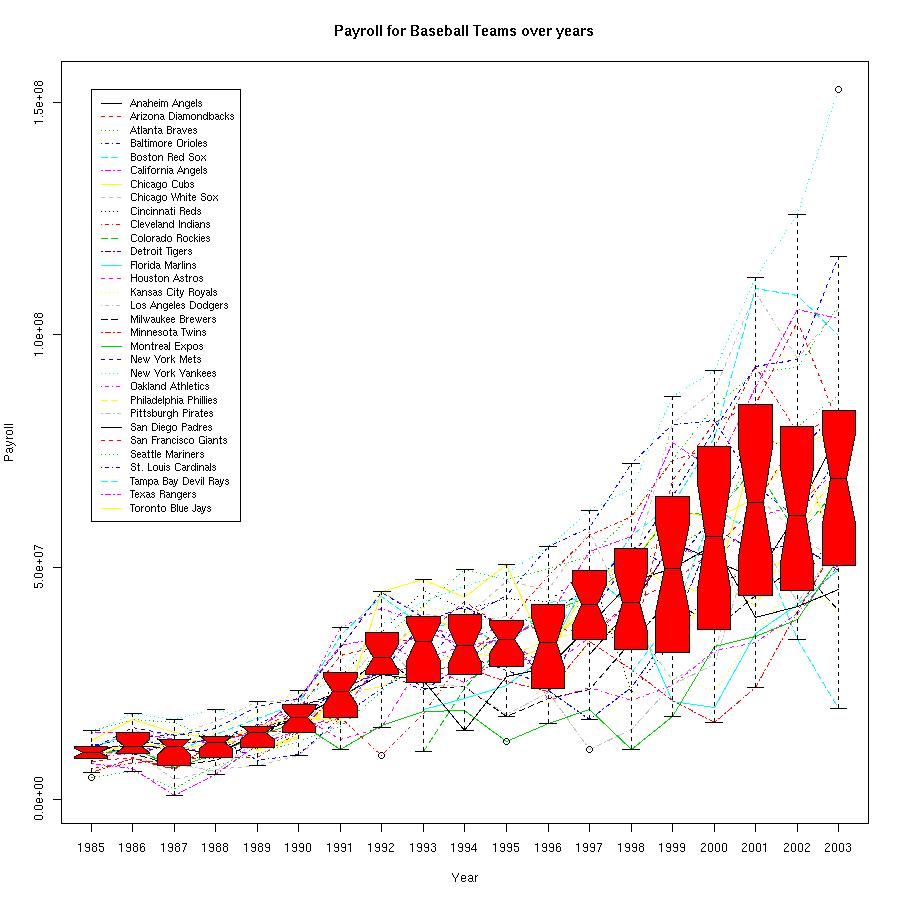
\includegraphics[width=5.5in]{RDBMS/images/PayrollYear.jpg}
 \caption{Time series plot for payroll with a boxplot for each year showing the distribution of the total payrolls for the collection of teams.}
\label{fig:payrollYear}
\end{figure} 
\end{center}

\begin{verbatim}
boxplot(Payroll ~ Year, data = d,at = 1985:2003, add = TRUE, 
        col="red", lwd=2, notch = TRUE)
plot(0, xlim = range(d[,"Year"]), ylim = range(d[,"Payroll"]), 
     type = "n", ..., xlab = xlab, ylab = ylab)

sapply(1:length(dd), function(i) {
        lines(dd[[i]][,"Year"], dd[[i]][,"Payroll"], col = i, lty = i)
        TRUE
        })

legend(min(d[,"Year"]), max(d[,"Payroll"]), names(dd), 
       col = 1:length(dd), lty = 1:length(dd), cex = .90)
\end{verbatim}

\begin{center}
\begin{figure}
 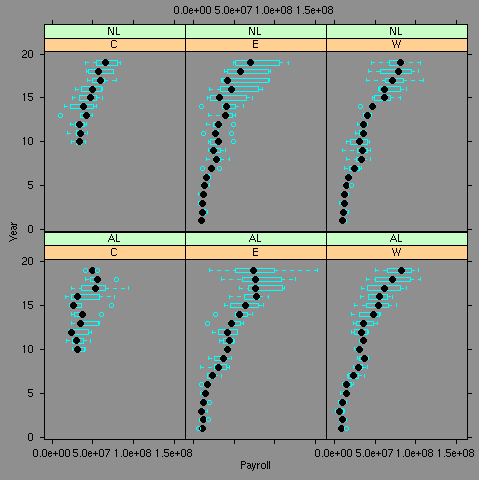
\includegraphics[width=5.5in]{RDBMS/images/PayrollPlotBW.png}
 \caption{A trellis/lattice-based boxplot of payroll versus year for each division with each of the two leagues (American and National)}
\label{fig:payrollYear}
\end{figure}
\end{center}

\begin{verbatim}
bwplot(Year ~ Payroll |  Division * League , 
       data = d, allow.multiple = TRUE)
\end{verbatim}

Augment the SQL statment above to include the following team
statistics for each season: the number of games in the season, the
number games won in a season, the information as to whether the
team won the division, wild card, league, or world series. To do
this you will need to join the table with the salaries with the
team table.

Use the xyplot in the lattice plot to explore the relationship
between payroll and performance. To do this, control for inflation
by cutting the data into six groups according to 3 year intervals,
and lay out six plots for these intervals. Construct a factor that
indicates whether the team won their division (or wild card),
league, or world series. The options are: no title, won division
or wild card but not league, won league but not the world series,
or won the world series.


\section{SQL for Statisticians}\label{dbms:sect:Smarties} 

Interfaces between statistical software and relational databases  
offer the opportunity to mix statistical analysis with
structured queries in flexible ways.
In fact, the flexibility poses the problem of determining 
where to do which computations: in SQL, in R, or split between
the two.
The choice depends on several issues, including
the available functionality in each environment,
the efficiency of the functionality in these environments, 
and the size of the data to be processed.

In this section we consider three examples: finding 
the three largest values of an attribute,
taking a random sample of tuples, and computing summary statistics
on grouped data. For each example, we present multiple solutions and
discuss the pros and cons of approach. 
We will use the RMySQL package to communicate in R with 
the database. 

\subsection{Ranking tuples}
Suppose we are interested in finding the the three highest 
salaries for baseball players in 2003.
The salary table in the baseball database is not very large.
We could easily pull the entire table into R 
and do all of the computations there.
\begin{verbatim}
sals = dbReadTable(con, "Salaries", row.names="playerID")
sort( unique( sals[sals$yearID == 2003,]$salary), 
      decreasing = TRUE)[1:3]
\end{verbatim}

Alternatively, the work can be done in SQL. As noted earlier,
the LIMIT clause can produce unreliable results when used with the
ORDER BY because of the order of operations, i.e. the limit is applied
before the tuples are ordered.  
The following SQL statement yields an ordered list of the distinct
values for salary:
\begin{verbatim}
orderSalary = dbGetQuery( con, 
     "SELECT DISTINCT Salary FROM Salaries 
        WHERE yearID = 2003 ORDER BY Salary DESC;" )
\end{verbatim}
Notice that we have pulled over all distinct salary values. 
An improvement on this approach uses dbSendQuery to avoid bringing
all of the sorted salary values into R.
\begin{verbatim}
res = dbSendQuery( con, 
      "SELECT DISTINCT Salary FROM Salaries 
         WHERE yearID = 2003 ORDER BY Salary DESC;")
topSalary = fetch( res, n = 3 ) 
dbClearResult( res ) 
\end{verbatim}

Celko provides an SQL solution to this problem that avoids sorting 
the salaries.
To understand it, it helps to think in terms of a sequence of nested subsets.
The goal is to assign a ranking to a subset of the table.
This subset contains the rows that have an equal
or higher value than the value that we are looking at.
Below, the Salary table with alias S1 provides the copy of the tuples 
to examine and the alias S2 provides the set of boundary values.
\begin{verbatim}
SELECT S1.Salary, 
     (SELECT COUNT(Salary) FROM Salaries AS S2
        WHERE S2.Salary > S1.Salary) AS Rank
  FROM Salaries AS S1;
\end{verbatim}

Another approach pulls the data into R in batches.
It finds the highest three salaries in a batch, and compares 
these salaries with the highest three in the previous batch. 
It is useful in the situation where we have more data than 
can easily fit in our R session or that can be sorted
in its entirety.
\begin{verbatim}
totCount = dbGetQuery( con, 
     "SELECT COUNT(*) FROM Salaries 
        WHERE yearID = 2003;")
res = dbSendQuery( con, 
     "SELECT Salary FROM Salaries 
        WHERE yearID = 2003;")

blockSize = 200
topSalary = NULL

for (i in ceiling(totCount[[1]]/blockSize)) {
    topSalary = sort( 
         unique( c(topSalary, fetch( res, n = blockSize)[[1]])),
         decreasing = TRUE )[1:3]
}

dbHasCompleted(res)
\end{verbatim}
Note that the last batch may be smaller than the blocksize
but the fetch will not give us an error when we ask for
more records than are left.
Note also that if our goal were to compute a median, 
this approach would not work.

If the ultimate goal is to find the players 
that correspond to the three highest salaries, we return to the 
database, and query the Salary table for the playerIDs that correspond
to the highest salaries (there may be more than three).
One way to do this, is to paste together a query that contains
the three salary values,
\begin{verbatim}
charSalary = paste( orderSalary[[1]][1:3], collapse = ", " )
cmd = paste( "SELECT playerID FROM Salaries WHERE yearID = 2003 
                 AND Salary IN (", charSalary, ") ;", sep = "" )
dbGetQuery( con, cmd )
\end{verbatim}

\subsection{Random sampling}
At times we want to work with a representative subset of the data.
For example, a graphic based on a subset may offer a clearer picture of
underlying patterns than one based on the entire data. 
SQL does not contain a pseudo random-number generator, and as shown
in Section~\ref{rng:sect:algorithm}, programming one from scratch
is not a good idea if you need a good random sampling procedure.
Sampling is a fundamental aspect of statistics, and so
well-tested pseudo random-number generators are a part of most 
statistical software. 
It appears that the selection process will need to be done in R. 
Even so there are many possible approaches to take.

Suppose we wish to take a sample of connections from the TCPConnections
table in the Network database.
Most simply, we can pull the key to the table across into R,
sample from it, and construct a query based on this sample
to get the corresponding records.

\begin{verbatim}
ConnID = dbGetQuery( con, "SELECT conn FROM TCPConnections;" )

sampleID = sample( ConnID$conn, 200)

sampleCharID = paste( sampleID, collapse = ", ")

sampleData =  dbGetQuery( con, 
                paste( "SELECT * FROM TCPConnections 
                        WHERE conn IN(", sampleCharID, " );", 
                        sep = "" ) )
\end{verbatim}

Two potential drawbacks to this approach arise: 
the entire index column is retrieved in order to sample from it,
and the set of sampled indices may get very long.  
We provide alternatives that address each of these possible problems.
First, if the key is an auto-increment type then it will have
values 1 through COUNT(*), and we can use this knowledge to 
generate the sample indices without having to pull the key attribute
into R.
\begin{verbatim}
totCount = dbGetQuery( con, "SELECT COUNT(*) 
                             FROM TCPConnections;" )
sampleID = sample( totCount, 2000)
\end{verbatim}
If the key is not such an index, one can be created with a temporary
table that consists of two attributes, the auto-increment index
and the original key attribute. 

\begin{verbatim}
 IDMatrix = matrix(sample(totCount, 2000), nrow = 10 )
 sampleData = apply( sampleMatrix, 1, function(x) 
               { 
                 charID = paste( x, collapse = " ," )
                 monte = dbGetQuery( con, paste( "SELECT * 
                         FROM TCPConnections 
                         WHERE conn IN (", charID, " );", sep = "" ))
                 summary(monte) 
               }
             )
\end{verbatim}

To address the second problem, we can reduce the size of the list of
indices to appear in the sample, which need to be in the IN clause 
of the SELECT query by pulling the sampled tuples across in batches.
This would be accomplished similarly to the approach shown in
the previous example.


\subsection{Summary statistics for grouped data}
Working with random samples of rows from a table is one
way to reduce the size of the data for analysis.
Another way is to aggregate like tuples.
In the study of network connections, we want to examine
the behavior of the connections over time for different ports. 
Rather than examine individual connections, attributes for
connections in the same time interval could be summarized 
and studied.  To make this concrete, we could examine 
the 0.25, 0.5, 0.75 quartiles and the maximum total packets
sent for connections to port 20 in 15 minute time intervals.
The code in Figure~\ref{dbms:fig:TCPbundle}
is one such approach.
The observed time period March 1, 1999 to April 8, 1999 is
cut into 15 minute intervals.
The data are ordered according to port and the time the 
connection was made to that port and placed in a temporary table.
This table holds only those attributes (and ports) of interest.
Records are fetched into R in blocks of 30,000 in port/time sequence.
The time the connection was sent is converted into a 15-minute
interval factor, and once converted, the tapply function does 
the work of finding the summary statistics on all connections in 
each 15-minute interval. 
These summary statistics are then appended to those computed 
so far, and another batch of records are fetched.
Note that one time interval will be split across two consecutive
batches of records. This incomplete interval needs to be saved
from one fetch to the next. We ignore that aspect of the
problem here.

\begin{figure}

\begin{verbatim}
# Initialize the date variables for pooling the data
  mintime = ISOdatetime(1999, 3, 1, 5, 0, 0)
  maxtime = ISOdatetime(1999, 4, 8, 3, 0, 0)
  timebreaks = seq.POSIXt(mintime, maxtime, by = "15 mins")

# Select the ports to examine
  Ports = c(20, 21, 22, 23, 25, 37, 79, 80, 113)

# Use SQL to create a temporary table that has the data sorted in
# port/time of first packet and that has only the variables of interest.
  dbGetQuery(con,"CREATE TEMPORARY TABLE short SELECT
     least(port_a,port_b) as port, 
     first_packet as timeSent, 
     (total_packets_a2b+total_packets_b2a) as totPackets 
     FROM TCPConnections order by port, timeSent ;")

# This function pulls data in blocks from the temporary table.  
# The data are then aggregated into 15 minute time intervals.
# Summary statistics such as the total number of connections,
# and the quartiles of total packets sent are computed for each interval.

processBlk = function (ports = Ports, inc = 40000)
{
    portstats = vector(mode = "list", length = length( ports ) )

    for (i in 1:length(ports)) {
        cmd = paste("SELECT * FROM short WHERE port IN (",ports[i],")  ;")
        cmd2 = paste("SELECT COUNT(*) FROM short WHERE port IN (",ports[i],") ;")
        recs = dbGetQuery(con,cmd2)
        res = dbSendQuery(con,cmd)
        
        n=inc
        while (n < recs + inc) {
            portData = fetch(res, inc)
            class(portData[["timeSent"]]) = c("POSIXt","POSIXct")
              tb = timebreaks[ min( portData[[ "timeSent" ]] ) <= timebreaks &
                     max( portData[[ "timeSent" ]] ) >= timebreaks ]
              timeFac = cut.POSIXt(portData[["timeSent"]],tb)

\end{verbatim}
\end{figure}

\begin{figure}
\begin{verbatim}

# Accumulate the summary stats
# The first statistic is the number of connections in the time interval

            numCon = tapply( portData[[ 3 ]], timeFac, length)
            notNAs = sapply(numCon, function(x) !is.na(x))
            rown = names( numCon )[ notNAs ]
            xx = matrix(( numCon [ notNAS ]), ncol = 1, byrow = TRUE)

            statQ = tapply( portData[[ 3 ]], timeFac, 
                     function(x) quantile( x, c(0.25, 0.5, 0.75, 1) ))

            xx = cbind(xx, matrix( unlist( statQ ), ncol = 2, byrow=TRUE))

            portstats[[ i ]] = rbind( portstats[[ i ]], 
                   as.data.frame(xx, row.names=rown))
            n = n+inc
         }
         dbClearResult(res)
  }
}
\end{verbatim}
\caption{describe the task}\label{dbms:fig:TCPbundle}
\end{figure}

%Do We want to show another way to do this?

%\subsection{Least Squares?}
%Do a least squares in batches? Updating ....

%Some calculation where numerical accuracy matters

\begin{comment}

\section{Managing and Designing your own Database}\label{dbms:sect:design}

As a statistician working on a project, you may face 
decisions on how to organize and manage the data in the project,
including whether or not to use a relational database 
management system.
The overhead in setting up a database is significant so there
need to be good reasons for choosing to use a database over
a project-specific organization of the data. 
In this section, we review some considerations to bear in mind 
when making this decision, and we discuss the basics of 
creating and designing databases. 


\subsection{Considerations}
A first consideration in the decision whether or not
to use a relational database is to determine who will be using the data.
If the only application using the data is your application, 
then organizing it in a form suitable for your needs 
may be the most efficient way to go and a database may be unnecessary. 
On the other hand, when several applications require access to
the data, each with a different set of requirements, then a centrally 
maintained database may be needed to guarantee data integrity.

A database management system enforces data integrity in a number of ways.
As seen already, checks can be placed on columns to ensure that the
data have the right type, have appropriate values, and are not NULL.  
The deletion of a row from one table can be automatically
reflected in other tables, or such changes can be forbidden in a 
particular table to maintain consistency across tables.
Further, transactions where multiple clients are updating a 
table simultaneously can be controlled to avoid data loss,
and these transactions can be ``rolled back" to restore the state of
a database before a user began his changes.

Another issue is security.  
Access to data can be controlled at the database, table, or column level. 
Use of the database may be restricted in scope and in privilege.
Scope restrictions control the host from which a user can connect to 
a database and and whether a password is required.
Restrictions on privileges control the types of commands or queries
that a user may perform, such as allowing a user to issue SELECT
statements, to create and delete tables, or to shutdown the server.

A relational database management system provides fast access to 
selected parts of large databases, and it provides powerful ways 
to summarize and tabulate data. So the size of your data should
be a factor in your considerations as well as the type of data that
need to be stored. 
If data are being collected from a variety of locations and analysis
of the data will be on-going throughout the data collection process
then having a system that supports the dynamic nature of this process
and that support applications for data entry could be real time saver.

The question of who will be maintaining the data also plays a role
in the decision whether or not to use a database. 
Clearly, setting up a database involves up-front costs.
However, personal database management systems are becoming widely 
available and no longer need a team of experts to set up and 
maintain.


\subsection{Setting up a database management system}

The database management system is a software application that 
does what its name implies, it manages databases. 
It runs a server as a daemon that listens for client 
requests for connections; 
it controls access to its databases, including
managing simultaneous users of the same database;
and  it performs administrative tasks such as logging activity
and managing resources.

MySQL is one such database management system. It is open source and
based on the SQL standard.  Detailed installation instructions appear
on the MySQL website, www.mysql.com, and in Butcher \cite{Butcher}.
You will need to decide which version (i.e. stable or Beta) to
download from the MySQL site to install and whether to install the
binary or the source.  These decisions depend on whether: you need a
stable production environment; your application requires features that
only appear in the Beta version; your system has an atypical
configuration; and you want special options in MySQL which would
require installation from source.

We outline the steps required to install MySQL from source on a Linux system.
In order to run, the MySQL server needs a Linux user and group which are both
called MySQL. We begin by creating these (as root), 
\begin{verbatim}
groupadd mysql
useradd mysql -g mysql
\end{verbatim}

After downloading the source, unzip and untar it into /usr/local/src. 
Then proceed to \executable{configure}, \executable{make}, and 
\verb+make install+ the application. 
To get started, you may want to configure with simple options such as
\begin{verbatim}
./configure --prefix=/usr/local/mysql
\end{verbatim}
The next step is to create a directory in which the data will
be stored. The script \executable{mysql\_install\_db} creates the directories 
and base files for managing the databases.
That is, the database management system uses a database to manage
its databases.
To set file permissions and system configurations 
MySQL provides some standard configurations that can be copied.
\begin{verbatim}
chown -R root /usr/local/mysql
chown -R mysql /usr/local/mysql/var
chgrp -R mysql /usr/local/mysql
cp support-files/my-medium.cnf /etc/my.cnf
\end{verbatim}

Now the server is ready to be started.
It runs a daemon called \executable{mysqld} that listens for requests 
for a connection to the database.
To start \executable{mysqld}, it is advisable to run the shell script
\executable{mysql\_safe} that will ensure that the server keeps running
if an error occurs.
\begin{verbatim}
/usr/local/mysql/bin/mysql_safe --user=mysql &
\end{verbatim}
If the server fails to start, the error messages should indicate
whether the problem is with file permissions or because the server is
already running or if there is some other error.
Once the server is running, the client program \executable{mysqladmin} 
administers the system, allowing you to shutdown or ping the server
and to set root password among other things.

\subsection{Setting up a database}
After installing the database management system, you can create 
a database.  Either the \executable{msyqladmin} program or SQL queries
can be used to create a database.
For example, to create the bank database, we can issue the 
following command at the Linux command line,

\begin{verbatim}
mysqladmin create BankDB -u nolan -p
\end{verbatim}
or we can invoke MySQL and then issue an SQL query as follows,
\begin{verbatim}
mysql -u nolan -p
CREATE DATABASE BankDB;
\end{verbatim}

Both of these statements create an empty database with no tables.
The next step is to add tables to the database. 
To do this, we must specify the attributes and their data types. 
The SQL queries below specify to use the BankDB database 
and to create the Customers table in that database.

\begin{verbatim}
USE BankDB;
CREATE TABLE Customers 
   (CustNo INT(4) NOT NULL, 
    Name CHAR(20), 
    Addr CHAR(30), 
    PRIMARY KEY (CustNo));
\end{verbatim}
In the table creation, we define the attributes and make 
the attribute CustNo the primary key.
Tables can be listed with SHOW TABLES; and attributes can
be listed via the DESCRIBE statement.

\subsubsection{Populating Tables}

Once a table is set up, we need to populate it with tuples. 
We can insert one tuple at a time with the INSERT statement. 
Alternatively, the LOAD DATA statement enables a text file 
containing data to be loaded in bulk into the database.
The \executable{mysqlimport} command (not an SQL query) can be 
used in a similar way. 
Below we show three versions of the INSERT statement.
The first provides an ordered list of values to be inserted
into a tuple, the second provides a list of attributes each
followed by their value, and the third provides a list of
attributes followed by a list of values in the same order as
the listed attributes.

\begin{verbatim}
INSERT INTO Customers VALUES (1,"Smith,J","101 Elm");
INSERT INTO Customers Addr = "101 Elm", CustNo = 2;
INSERT INTO Customers (CustNo, Addr) (3, "17 Spruce");
\end{verbatim}

\subsubsection{Consistency}\label{dbms:sect:consistency}
When we create multiple tables we typically need to connect a
record in one table to a record or records in another table.
In the bank example, the attribute CID in the Registration
table is a key to the customers in the Customer table.
For this reason, we call CID a foreign key.  
At the time a table is set up, we can place 
restrictions on changes that can be made to a key in a table 
and how changes in one table are to be reflected in another.
For example, in the query below, we set up the Accounts table
where AcctNo may not be set NULL and Branch may hold only two 
possible values (``City" and ``Suburb").
In addition, AcctNo serves as the primary key for the table,
and the attribute Branch references the Branch attribute in the 
Branches table. 
Changes to Branch in the Branches table have been constrained as
follows: 
when the value for Branch is changed in the Branches table, 
then the change will ``cascade" to the Accounts relation, 
i.e. it will change correspondingly, 
and when a tuple is deleted in the Branches table then the 
those tuples with the same value for Branch in the Accounts table 
will be set to NULL.

\begin{verbatim}
CREATE TABLE Accounts 
       (AcctNo INT(6) NOT NULL,
        Balance FLOAT(10,2), 
        Branch CHAR(8) CHECK (TYPE="City" or TYPE="Suburb"),
        PRIMARY KEY (AcctNo)
        FOREIGN KEY (Branch) REFERENCES Branches(Branch)
               ON UPDATE CASCADE ON DELETE SET NULL;
\end{verbatim}

Once a table has been created, the ALTER statement may be used to 
make changes to the table definition. Columns can be added, changed,
dropped, and renamed.  Keys can be added and tables themselves can
be renamed. Below is an example where the data type of an attribute
in the Branches table is modified.

\begin{verbatim}
ALTER TABLE Branches MODIFY Address CHAR(30);
\end{verbatim}

\subsubsection{Handling transactions and elimination of records}
The specifications in the declaration of a table helps maintain
integrity of the data in the table. For example, if an attribute
is specified as a primary key, then a tuple containing a
duplicate entry for the primary key can not be inserted into the
table.  Further, when the value of a primary key is changed in a
table, these changes are reflected in other tables provided the
specifications are given as shown in Section~\ref{dbms:sect:consistency}.
To change data that has already been entered into a table, 
we can update it as follows,

\begin{verbatim}
UPDATE Accounts SET AcctNo = 101 WHERE AcctNo = 201;
\end{verbatim}

At times we want to eliminate an entire database or table.
The DROP statement allows us to do this.
If we only need to remove a subset of tuples in a table then
we use the DELETE statement.

\begin{verbatim}
DELETE FROM Accounts WHERE AcctNo in (302, 201);
\end{verbatim}

\subsubsection{Access, Privileges, Security}
To allow users other than the one who set up the database to access 
the data, we need to GRANT privileges to them.
One common type of privilege to grant allows a user to only perform 
SELECT queries.
The following statement gives the user \SName{nolan} permission to 
issue SELECT queries
on all tables in the BankDB database when connected from the local host.

\begin{verbatim}
GRANT SELECT ON BankDB.* TO nolan@localhost;
\end{verbatim}

At the other extreme, a user may be given the privilege to perform
all types of queries on a database except for the GRANT. 
The following GRANT gives the nolan user all privileges, except GRANT,
on all tables in the BaseballDatabank database when connecting from any host 
provided that password npass is supplied. 

\begin{verbatim}
GRANT ALL ON BaseballDatabank.* TO nolan@"%" 
                 IDENTIFIED BY "npass";
\end{verbatim}

The MySQL database holds the grant table that control the 
privileges for the users of databases on the client.  
It is called \SQLName{mysql} and contains five tables that control 
privileges at five different levels: \SQLName{user, db, host, tables\_priv, 
and columns\_priv}.

Privileges can be ascertained from the 
\begin{verbatim} SHOW GRANTS FOR nolan@"%";\end{verbatim}
and they can be revoked with the REVOKE statement.
In order to connect to the database, the user must be present in the
\SQLName{user} table.
There privileges can be set for all databases on the server.
For example, a user may be given SELECT privileges on all databases.
If the SELECT privilege in not granted at this level,
when a user attempts to SELECT from a table in a particular database
then the \SQLName{db} table is checked to see if that privilege
is granted on that database.
Continuing in this way, if permissions are not given at the
database level, we proceed to the table level, which appears in
the \SQLName{tables\_priv}, and then on to the column or attribute level
permissions found in \SQLName{columns\_priv}.



\subsection{Designing Schema}
Database design is the process of deciding how to organize data 
into tables and records and how the tables will relate to each other.
The database should mirror the organization's data structure and process 
transactions efficiently.

We consider an example from a hypothetical survey of health and dietary 
habits of teenage girls. 
To develop a schema for the survey data, we first consider the 
survey process, and identify where definable events occur, 
e.g. the initial survey, visits to the doctor, etc.  
The survey will be ongoing over several years, where high school 
students are chosen to participate in the survey according to a two-stage 
sampling approach. In the first stage, a set of high schools are chosen at 
random, then in the second stage a random sample of students are selected
from each high school.  
This sampling occurs in waves over the course of several years.
The students in each wave complete an introductory
questionnaire, keep track of the food they eat each day in diaries 
over several months, and have scheduled checkups with their doctors.
In addition, teachers fill out questionnaires giving their views on
the participating students. 

From this brief description of the survey, two entities immediately
surface: the student and the high school.
It seems natural to have a table containing information on the 
students surveyed.
This may contain the student's name, address, and high school, 
demographic data such as age, grade-level, race, and family income, 
the food diary, lab tests from the doctor visits, and 
teacher interviews about the students.
The high school entity might simply contain the high school name and address.

\begin{figure}
\begin{verbatim}
Smith,J  101 Elm        Jefferson High 
 Day 1: 1300    Day 2: 1900     Day 3: 2100 ... Day 17: 1900  
 Visit 1: 29.7  Visit 2: 29.8   
 Dr. Reed, X Medical Group      
 Ms Martin      7.5   

Brown,D  12 Oak         Jefferson High 
 Day 1: 1100    Day 2: 2100     Day 3: 2300 ... Day 15: 1700  
 Visit 1: 18.1  Visit 2: 18.8   
 Dr. Reed, X Medical Group      
 Ms Martin: 5.5  Mr Green: 4.8   

Ritter,L         2015 Main              Highland High 
 Day 1: 1900    Day 2: 2000     Day 3: 2100 ... Day 21: 1400  
 Visit 1: 24.1  Visit 2: 23.8   Visit 3: 23.5   
 Dr. Eisen, Y Family Practice   
 Ms Max: 9  

\end{verbatim}
\caption{Data in a ragged array from a hypothetical sample survey. 
Notice that the number of calories consumed were recorded for a varying number
of days for each participant, and the number of doctor visits and teacher
reviews is not constant across participants.}\label{dbms:fig:CTragged}
\end{figure}

An oversimplified version of the student data appears in 
Figure~\ref{dbms:fig:CTragged}. 
The data contain information on three hypothetical students in the survey.
There we see the student's daily calorie consumption,
Body Mass Index recorded at doctor's visit, the doctor's name and clinic, 
and the teacher's name and numeric evaluation.
Notice that these data form ragged arrays. That is, students do not record
their calorie intake for the same number of days, they do not all visit the
doctor the same number of times, and they do not all have the same number of 
teacher evaluations. A database table must be rectangular, i.e. it must
have the same number of columns in each row. We do not have this in our 
survey data.  
This problem can be addressed by including in each student's record
say 30 daily diet columns, six doctor visits columns, and three teacher 
evaluation columns, where 30, six, and three are chosen as upper limits
on the number of days, doctor visits, and teacher evaluations, respectively. 
Several drawback to this approach immediately surface: 
student records would typically have many empty cells for most do not 
use the maximum allowed for these activities, 
but a student might unexpectedly exceed the maximum number of columns allowed.
A better approach would be to recognize that these ragged arrays
each represent an entity, namely a daily diet, a visit to the doctor, 
and a teacher's evaluation. 
Therefore each deserves its own table. 

Take for example the doctor visits.  A doctor-visit table
could be designed as in Figure~\ref{dbms:fig:visits}, 
where the data for the doctor's visits has been split off from the 
student record in Figure~\ref{dbms:fig:CTragged} into a separate table.
Note however that two problems have arisen, the doctor's name is 
redundant as it now appears in each visit tuple and the connection between
the student and the visits to the doctor has been lost.
We remedy the second problem by adding to the visit table an 
attribute that identifies the student. 
Rather than use the student's name, it is more suitable to
add a student identification number to the table because 
names and other personal data for participants in surveys 
are often kept confidential.
Instead of putting this confidential information in many tables,
it makes sense to keep it in one table, to identify individuals by an
uninformative identification number, and to place security constraints
on the single table with names. 

\begin{figure}
Doctor Visit \\
\begin{tabular}{llll}
Date & Lab results & Doctor & Clinic\\
1& 19.7  & Dr. Reed & X Medical Group\\  
2& 19.8 &  Dr. Reed  & X Medical Group\\
1& 18.1 &  Dr. Reed & X Medical Group\\ 
2& 18.8 &  Dr. Reed & X Medical Group\\ 
1& 21.1 &  Dr. Eisen & Y Family Practice\\
2& 20.8 &  Dr. Eisen & Y  Family Practice\\
3& 20.5 &  Dr. Eisen & Y Family Practice\\
\end{tabular}
\caption{The data for the doctor's visits has been split off into 
a separate table. 
Note however that two problems arise, the doctor's name is redundant
appearing in each visit and the connection between 
the student and the visits to the doctor has been lost.}\label{dbms:fig:visits}
\end{figure}

That leaves the problem of redundancy of the doctor's name and 
clinic in the Visits table.
One doctor oversees many visits for a single student so it makes more 
sense to identify the doctor in the student table. 
This removes the redundancy from the visit table, 
but if we include the doctor's name and location in the student file, 
we still have redundant information. 
A doctor sees many students, and the doctor's clinic is information
about the doctor, not about the student. 
That is, we have identified another entity, the doctor.
A doctor table would contain, a doctor's identification number,
name, and clinic. The doctor's identification number would 
then appear in the student table to connect her with the students she treats.
The schema for the revised Visits table, the new Doctor table, 
and the Student table all appear in Figure~\ref{dbms:fig:schema}.
We see there that we also need a diary table and an evaluation table to hold 
the data in the diary entries and the teacher evaluations.

\begin{figure}

Students\\
\begin{tabular}{|lll|}
\hline
StudentId &  &  \\
Name &  &  \\
Address &  & \\
DoctorID &  & \\
HighSchool &  & \\
\hline
Diary & 0 & N\\
Visits & 0 & N\\
Evaluations & 0 & N\\
\hline
\end{tabular}

\medskip

Diary Entries\\
\begin{tabular}{|lll|}
\hline
StudentId &  &  \\
DayId &  & \\
Calories &  & \\
\hline 
Students & 1 & 1 \\
\hline
\end{tabular}

\medskip

Evaluations \\
\begin{tabular}{|lll|}
\hline
StudentId &  & \\
TeacherId &  &  \\
Score &  &  \\
\hline
Students & 1 & 1\\
Teachers & 1 & 1\\
\hline
\end{tabular}

\medskip

Visits \\
\begin{tabular}{|lll|}
\hline
StudentId &  &  \\
VisitId &  & \\
BMI &  & \\
\hline 
Students & 1 & 1 \\
\hline
\end{tabular}

\medskip

Doctors \\
\begin{tabular}{|lll|}
\hline
DoctorId &  & \\
Name &  & \\
Clinic &  &  \\
\hline
Students & 1 & N\\
\hline
\end{tabular}

\medskip

Teachers \\
\begin{tabular}{|lll|}
\hline
TeacherId &  &  \\
HighSchool &  & \\
Name &  & \\
\hline
Evaluations & 0 & N\\
HighSchool & 1 & N\\
\hline
\end{tabular}

\medskip

HighSchool \\
\begin{tabular}{|lll|}
\hline
Name &  &  \\
Address &  & \\
\hline
Teachers & 1 & N\\
Students & 1 & N\\
\hline
\end{tabular}

\caption{In this figure there is one ``table" for each entity, and in this 
table the attributes are listed.
Also connections to other entities are displayed. 
For example, within the Patient entity, we see that one patient may
have no tuples in the Visit table, one tuple, or many tuples.}\label{dbms:fig:schema}

\end{figure}

Finally, consider the relationship between teachers and high schools.
This relation is many-to-many meaning that one high school has
many teachers and on teacher may teach in many high schools.
Thus a teacher-high school entity, 
where each tuple is uniquely identified by the teacher-high school
pair, is required to handle this many-to-many relation. 
These types of tables are sometimes called linking tables.
It appears in Figure~\ref{dbms:fig:schema}. 

Figure~\ref{dbms:fig:schema} lays out the schema for the
database, where each entity is identified along with its attributes 
and its relations to the other entities.
The pair of numbers that follows the related tables 
specifies bounds on the number of tuples in these tables that 
a tuple in the given table may have.
For example, in the Student entity, we see that one student may
have between 0 and many tuples in the Visit table, whereas 
a visit instance in the Visits relation must have one and only one
student entity. 
Thus we identify the many to one relation between students and visits.

By describing the survey process, removing ragged arrays and redundancies
of the two types we encountered, we have arrived at a reasonably well designed
schema that is in what is called third normal form.  
Normal forms are essential for efficient data processing. 
See Rolland \cite{Rolland} for more details on normal forms.
                                                                      

\section{Alternatives to Databases}

Relational database tables are neither spreadsheets nor files.  In a
spreadsheet, cells in a workbook can contain instructions rather than
data; there is no conceptual difference between a row and a column,
i.e. they can be transposed; and the spreadsheet can be navigated with
a cursor.

Factors to consider: setup, maintenance, scale

As for flat files, the fields in a file are defined in the program,
not in the file itself; files are processed one line at a time,
whereas in a relational database we connect to a a suite of tables and
work with the table as a whole entity; empty tables are still valid
tables for performing operations, while an empty file typically
requires special treatment, e.g. an EOF flag to handle clean up.

\cite{Celko}
%[[Reference SQL for Smarties]]


Flat files, file systems, XML, Object databases, etc.



\putbib[RDBMS/dbms]
%\cite{Celko}
\end{bibunit}
\end{comment}

\section{Exercises}

The following exercises all use the baseball databank.

\begin{enumerate}
\item How many people are included in the databases?
\item Are all of these players? How many are players? how many are managers? and how many are both?
\item     What is the earliest season recorded in this database? and the most recent?
\item  What college produced the largest number of major league baseball players? Is there a geographical trend? How many colleges are there in total? And how many players didn't go to college at all?
\item  Can we tell who won the "World" series in a given year?
\item  Who lost the "World" series in each year?
\item Look at the relationship between the number of games won in a season and winning the world series? And similarly relate these to payroll.
\item  Plot the payrolls over years for the different teams. What plot types are good for showing this data? Contrast different graphical techniques. Information for inflation rates from 1986 to the present is available in the database inflation and in the relation AnnualRates. You might consider using this to adjust/control the dollar amounts for inflation.
      Superimpose the payroll of the two teams that made it to the "World Series" on this plot. Is there a relationship? How about for the teams that made it into the playoffs in a year?
\item Show the distributions of the payrolls over years. We can think of a boxplot for each year for this. Again, we can superimpose additional attributes and even lines connecting the different statistics for particular teams if they are not very noisy.
\item  Look at the payrolls for the teams that are in the same leagues? and then in the same divisions? Are there any interesting characteristics?
\item Is the payroll related to the age of the players? One might expect an old team to be paying veteran players a lot near the end of their careers. Teams with a large number of older players would therefore have a large payroll. Is there any evidence supporting this?
\item Look at the distribution of salaries of individual players over time for different teams.
\item Look at players and see whether the distribution of home runs has increased over the years?
\item Are Hall of Fame players, in general, inducted because of rare, excellent performances or years or are they rewarded for consistency over years?
\item Are certain baseball parks better for hitting Home Runs? Can we tell from this data? Can we make inferences about this question?
\item Do teams with a few good players and many mediocre players tend to do better than a team made up of more homogeneous talent?
\item Look at the distribution of how well batters do. Does this vary over the years? Do the same players excel each year? Is there a clustering? a bi-modal distribution?
\item Do pitchers get better with age? Is there an improvement and then a fall off in performance? And is this related to how old they are? the number of years they have been pitching? which league they are in and the designated hitter rule? Do we have information about each of these factors and how can we combine them to present information about the general question?
\end{enumerate} 

%\bibliographystyle{plain}
%\bibliography{RDBMS/dbms}
 
\setcounter{chapter}{10}

\chapter{Graphics}

A series of examples that introduce some modern visualization topics.


\section{Election Maps}

\section{Internet Mashup}

Google Earth

\section{Lattice }


\section{Collaborative Visualization}

ManyEyes

Swivel

\section{Visualizing Large amounts of data}

\section{Animation}

SVG

Processing

\section{Dynamic Graphics}

Ggobi


 
\setcounter{chapter}{11}
\def\Title#1{\textit{#1}}
\def\SCode#1{\Rcode{#1}}
\def\SVariableName#1{\Svar{#1}}
\def\SValue#1{\texttt{#1}}
\def\Email#1{\texttt{#1}}
\def\TabChar{\\t}
\def\NewLineChar{\\n}


\chapter{SPAM: A case study}
%\chapter{Case-Study: Classifying SPAM emails}
\section{Introduction}
 
When we read an electronic-mail message, it is often immediately
obvious to us whether the message is spam or not.  Most of the time we
need only look at the subject line of the message to determine that it
is spam.  But what is not immediately obvious is how to design an
automatic procedure to save us the hassle, time, and irritation of
having to delete ``by hand'' unwanted messages.  In this chapter, we
examine two statistical approaches to classifying electronic-mail
messages as spam or not.

One approach finds the chance a message is spam by looking at which
words are found in the message and which words are absent from it.
This probability-based approach begins by studying the words found in
a large collection of electronic-mail messages which have already been
classified as spam or ham (i.e. not spam).  Then when a new message
comes to us, we use the information gleaned from our ``training'' set
to compute the probability that the message is spam based on the words
appearing in the new message.  We use the naive Bayes method to
compute these probabilities.

The other approach finds the messages in the training set that are
closest to the new message to be classified, and if the majority of
these messages are spam then that message will be classified as spam.
To find close messages, we compute the distance between messages using
particular characteristics, such as the percent of characters in the
message that are capital letters, whether or not the subject line of
the message contains ``Re:'', and the number of attachments.  Then we
find the $k^{th}$ nearest training messages to our new one and use
them in the classification, i.e. if our new message is close to more
spam than ham messages then the new message is classified as spam.
This technique is called $k^{th}$ nearest neighbor classification.

For both of these approaches, we need to ``tune'' the method.
That is, for the naive Bayes method, we must determine a threshold 
for the probability of interest, i.e. for the probability that the message
is spam.
Then a new message is classifed
as spam when the computed chance that it is spam falls above that level, 
otherwise we classify the message as ham.  
To tune the nearest-neighbor method, we must choose $k$, the number of
messages to include in the neighborhood. 
We use the technique of cross-validation to tune these methods.
In addition, we examine the behavior of these classifiers on
a new set of data that has been held in reserve, i.e. not used in the 
training nor in the tuning.

For this case study, we have mail messages from the Spam Assassin website 
\\
\URL{http://spamassassin.apache.org/}.
Altogether, there are five sets of messages: three contain regular
mail (ham) and two contain spam.  Each message is in its own file, and
there are about 9,000 messages in all.  The Spam Assassin Web page,
\URL{http://spamassassin.org/publiccorpus/},
gives a description of the naming convention for the files.

For our first task, we convert the raw text data into an R structure for 
future analysis. 
To do this we consider the following questions:

\begin{itemize}
  \item How should the data be organized?
  \item How do we test our code?
  \item How do we handle special cases?
\end{itemize}

Once the data are in an R structure we begin the application of 
one of the methods. 
For the nearest-neighbor data, we must further process the data
to form quantitative and categorical variables. 
In this process we face several questions,

\begin{itemize}
   \item How do we define a variable?
   \item What is considered a missing value?
   \item How do we check that the variable created is correct?
   \item How do we define a distance between messages based on these variables?
\end{itemize}

On the other hand, for the naive Bayes method, we must further
clean and process our data into a dictionary of sorts. This 
poses its own challenges, 

\begin{itemize}
    \item How do we build a dictionary?
    \item How can we represent the words found in a message in a 
    quantitative way?
    \item How do we check the conversion of text into this quantity?
\end{itemize}

In addition, we address issues common to both approaches, such as 

\begin{itemize}
  \item How do we address efficiency with regard to memory, 
  processing time, and space?
  \item How can we determine whether a method works well or not, and 
  how can we figure out why it works or does not work?
  \item What trade-offs do we face in writing our own high-level code, 
   using other high-level functions and packages, and writing C code?
\end{itemize}

We will address these questions as we work through the main tasks.
We then move on to what has traditionally been considered statistical
work: applying the method, tuning the parameters, and analyzing the
performance of the method on a new set of data.
But, before proceeding, we review how electronic mail works.

\section{The Anatomy of an E-mail message}

Electronic mail, usually called e-mail, consists of simple text
messages -- a piece of text sent to a recipient via the internet.  An
e-mail message consists of two parts, the header and the body.  The
body of the e-mail message is separated from the header by a single
blank line.  When an attachment is added to an e-mail message, the
attachment is included in the body of the message.  Even with
attachments, e-mail messages are still only text messages.

\subsection{The E-mail Header}

The header contains information about the message such as
the sender's address, the recipient's address, and the date of 
transmission.
This information is relayed in a special format 
that consists of  KEY:VALUE pairs.
Below is a sample header from a message found on the
SpamAssassin website.

\begin{verbatim}
Return-Path: whisper@oz.net
Delivery-Date: Fri Sep  6 20:53:36 2002
From: whisper@oz.net (David LeBlanc)
Date: Fri, 6 Sep 2002 12:53:36 -0700
Subject: [Spambayes] Deployment
In-Reply-To: <LNBBLJKPBEHFEDALKOLCIEJABCAB.tim.one@comcast.net>
Message-ID: <GCEDKONBLEFPPADDJCOECEHJENAA.whisper@oz.net>
\end{verbatim}
                                                                               
Notice the keys are Return-Path, Delivery-Date, From, Date,
Subject, In-Reply-to, and Message-ID. 
The value follows the keyword.
For example, in the above header, the value of the From key 
is \\
\texttt{whisper{at}oz.net (David LeBlanc)}.

Some of these keys are mandatory such as \Email{Date, From}, and \Email{To} 
(or \Email{In-Reply-To}, or \Email{Bcc}).
Other keys are optional but widely used, such as \Email{Subject, Cc, 
Received}, and \Email{Message-ID}.
Many keys are ignored by the mail system, but the entire header 
is relayed on to the recipient's server whether or not it is 
recognized. 
For example, keys starting with ``\Email{X}-'' are for personal application 
or institution use and are ignored by other applications.
The \Email{Received} header lines are important because they allow
the message to be tracked. As a message makes its way to the
intended recipient, servers add additional \Email{Received} lines
to the header. 


Below are some typical header keys:

\begin{itemize}
\item \Email{Message-Id}: a unique identifier for the message, assigned by the 
originating server; 
\item \Email{Return-Path}: specifies the sender's address and  
        bounced mail gets sent to this address;
\item \Email{Date}: added by the e-mail client;
\item \Email{Cc}: lists the recipients of a ``carbon copied'' message;
\item \Email{Reply-To}: the address set by the sender to which the 
recipient can reply; 
\item \Email{MIME-Version}: used for encoding binary content as attachments.
\end{itemize}

A value may be continued on a second line of the header, in which
case the line will be indented and begin with a tab character or
blank spaces.

\subsection{E-mail Attachments}

An Internet standard called MIME, 
Multipurpose Internet Mail Extensions, 
specifies how messages may be formatted and how to separate 
the attachments from the message. 
Information about the MIME encoding is provided through header fields, 
which are specified in an RFC. 

The Content-Type key is used to describe the content of a component
or of the entire body. 
The value provides the top-level type and subtype using the 
syntax:  
\begin{verbatim}
top-level/subtype; parameter.
\end{verbatim}
Parameters may be required or optional.
Below is an example of a content-type where the 
top-level is \Email{multipart}, which indicates there will be several 
documents in the body of the message, the \Email{mixed} subtype tells
us that the documents may be of different types, and the \Email{boundary}
parameter provides a special character string for delimiting the
start and end of the message parts.
\begin{verbatim}
Content-Type: multipart/mixed;
      boundary="----=_NextPart_000_00DE_01511A02.DB1A02A0"
\end{verbatim}
The Content-Type field in this example tells the receiving 
e-mail program that this message has more than one component, and each 
component will be separated by the string of characters 
\begin{verbatim}----=_NextPart_000_00DE_01511A02.DB1A02A0\end{verbatim}
The boundary string marks the beginning of each component.
It is prefaced with two additional hyphens in all instances.
The boundary string is also used to denote the end of the message, 
where it is both prefaced by two hyphens and followed immediately by two 
hyphens. 
The receiving email program knows when the last component of the message
has been read when it reads the boundary string with two additional
hyphens on either end of the string,
\begin{verbatim}------=_NextPart_000_00DE_01511A02.DB1A02A0--\end{verbatim}
Each component of a message must be prefaced by the boundary string
and a blank line. 
It may also contain MIME information.
If the blank line is missing, the recipient's e-mail client may have 
difficulty telling where the header information stops and the text of the 
message begins.

There are seven top-level types of attachments: text, image, audio, video, application,
multipart, and message.  Other examples of Content-Type values follow:

\begin{verbatim}
Content-type: text/html; charset=euc-kr;
Content-Type: application/zip; name="testFile.zip"
\end{verbatim}
The first example indicates that the message is in HTML format using a
Korean character set.  The second indicates that the component
is a zip file, and the sender named it \File{testFile.zip}.
Binary files (such as a compressed archive) can be
sent as attachments. 
In such cases, the sender's software must first encode the binary
file so that it can be sent over the Internet. 
One common encoding scheme is known as base64. 

We conclude by providing two sample e-mail messages.
The first is a plain text e-mail with no
attachments.  It consists of an instructor's response
to an e-mail inquiry sent by a student. 
The second e-mail message consists of a text message and two attachments 
sent by a student to the instructor. This e-mail message has then been 
forwarded by the instructor to the teaching assistant.
The three periods at the end of each attachment indicates
that only part of the attachment has been displayed.
The first attachment is a pdf file and the second is an HTML file.
The forwarded message is a plain text file.

\begin{figure}

%\framebox{
{\small{
\begin{verbatim}
 
From nolan@stat.Berkeley.EDU Mon Feb  2 22:16:19 2004 -0800
Date: Mon, 2 Feb 2004 22:16:19 -0800 (PST)
From: nolan@stat.Berkeley.EDU
X-X-Sender: nolan@kestrel.Berkeley.EDU
To: Txxxx Uxxx <txxxx@uclink.berkeley.edu>
Subject: Re: prof: did you receive my hw?
In-Reply-To: <web-569552@calmail-st.berkeley.edu>
Message-ID: <Pine.SOL.4.50.0402022216120.2296-100000@kestrel.Berkeley.EDU>
References: <web-569552@calmail-st.berkeley.edu>
MIME-Version: 1.0
Content-Type: TEXT/PLAIN; charset=US-ASCII
Status: O
X-Status:
X-Keywords:
X-UID: 9079
  
Yes it was received.
 
-------------------------------------
 
On Mon, 2 Feb 2004, txxxx wrote:
 
> hey prof .nolan,
>
> i sent out my hw on sunday night. i just wonder did you receive it.
> because i am kinda scared thatyou didnt' receive it.
> like i just wonder how do i know if you got it or not, since the cal
> mail system is kinda weird sometimes.  thanks
>
> txxxx
>
\end{verbatim}    
} }
% }
\caption{Sample email message with no attachments. The header includes fourteen
key:value pairs.  Note the \Email{Date} key includes a time-zone offset,
the \Email{Message-ID} key gives the unique ID to track the
mail from the \URL{stat.berkeley.edy} mail server,
the \Email{Content-Type} key indicates it is a plain text message
with no sttachments, and thre are four \Email{X-} keys.}\label{fig:simpleEmail}
\end{figure}


\begin{figure}
{\footnotesize{
\begin{verbatim}
From nolan@stat.Berkeley.EDU Mon Feb  2 22:18:56 2004 -0800
Date: Mon, 2 Feb 2004 22:18:55 -0800 (PST)
From: nolan@stat.Berkeley.EDU
X-X-Sender: nolan@kestrel.Berkeley.EDU
To: Gang Liang <liang@stat.Berkeley.EDU>
Subject: Assignment 1 sorry (fwd)
Message-ID: <Pine.SOL.4.50.0402022218470.2296-201000@kestrel.Berkeley.EDU>
MIME-Version: 1.0
Content-Type: MULTIPART/Mixed; BOUNDARY="_===669732====calmail-me.berkeley.edu===_"
Content-ID: <Pine.SOL.4.50.0402022218471.2296@kestrel.Berkeley.EDU>
Status: RO
X-Status:
X-Keywords:
X-UID: 9080
 
--_===669732====calmail-me.berkeley.edu===_
Content-Type: TEXT/PLAIN; CHARSET=US-ASCII; FORMAT=flowed
 
Content-ID: <Pine.SOL.4.50.0402022218472.2296@kestrel.Berkeley.EDU>
\end{verbatim}
}}
\caption{This sample email (split over two figures) has two
  attachments, a PDF file and an HTML file.  The \Email{Content-Type}
  key indicates that the attachments are separated by
  \Email{\_===669732====calmail-me.berkeley.edu===\_} with a
  \Email{--} prefix.  The first part of the email body is the a
  forwarded message.  Note that it has its own header indicating the
  content type is plain text.  Next is a PDF attachment which the
  owner has named \FileName{PLOTS.pdf}, and the third part is an HTML
  attachment.  Both attachments are encoded in base64.  }
\end{figure}

\begin{figure}
{\footnotesize{
\begin{verbatim}

---------- Forwarded message ----------
Date: Mon, 02 Feb 2004 21:50:47 -0800
From: Yyyy Zzz <Zzz@uclink.berkeley.edu>
To: nolan@stat.Berkeley.EDU
Subject: Assignment 1 sorry
 
I am sorry to send this email again, but my outbox told me that 
the last email only send 1 attached file. 
I am send ing this again to make sure you recieve the all 
the necessary files.
Thank You and sorry for the inconvenience.
  
--_===669732====calmail-me.berkeley.edu===_
Content-Type: APPLICATION/PDF; CHARSET=US-ASCII
Content-Transfer-Encoding: BASE64
Content-ID: <Pine.SOL.4.50.0402022218473.2296@kestrel.Berkeley.EDU>
Content-Description:
Content-Disposition: ATTACHMENT; FILENAME="PLOTS.pdf"
 
JVBERi0xLjEKJYHigeOBz4HTDQoxIDAgb2JqCjw8Ci9DcmVhdGlvbkRhdGUgKEQ6MjAwNDAy
MDIxMTIwMTEpCi9Nb2REYXRlIChEOjIwMDQwMjAyMTEyMDExKQovVGl0bGUgKFIgR3JhcGhp
Y3MgT3V0cHV0KQovUHJvZHVjZXIgKFIgMS44LjEpCi9DcmVhdG9yIChSKQo+PgplbmRvYmoK
...
 
--_===669732====calmail-me.berkeley.edu===_
Content-Type: TEXT/HTML; CHARSET=US-ASCII
Content-Transfer-Encoding: BASE64
Content-ID: <Pine.SOL.4.50.0402022218474.2296@kestrel.Berkeley.EDU>
Content-Description:
Content-Disposition: ATTACHMENT; FILENAME="Stat133HW1.htm"
  
PGh0bWwgeG1sbnM6bz0idXJuOnNjaGVtYXMtbWljcm9zb2Z0LWNvbTpvZmZpY2U6b2ZmaWNl^M
PGh0bWwgeG1sbnM6bz0idXJuOnNjaGVtYXMtbWljcm9zb2Z0LWNvbTpvZmZpY2U6b2ZmaWNl^M
Ig0KeG1sbnM6dz0idXJuOnNjaGVtYXMtbWljcm9zb2Z0LWNvbTpvZmZpY2U6d29yZCINCnht^M
...

--_===669732====calmail-me.berkeley.edu===_--
    
\end{verbatim}
}}
\caption{This sample email (split over two figures) has two
  attachments, a PDF file and an HTML file.  The \Email{Content-Type}
  key indicates that the attachments are separated by
  \Email{\_===669732====calmail-me.berkeley.edu===\_} with a
  \Email{--} prefix.  The first part of the email body is the a
  forwarded message.  Note that it has its own header indicating the
  content type is plain text.  Next is a PDF attachment which the
  owner has named \FileName{PLOTS.pdf}, and the third part is an HTML
  attachment.  Both attachments are encoded in base64.  }
\end{figure}

\section{Converting raw text data into an R structure}
Whether it be naive Bayes classification or $k^{th}$-nearest
neighbor, the first task we face is to convert the raw text data into 
an R structure for further processing and analysis.

\subsection{Organizing the Data}
To get started we want to think about what we want to end up with
in terms of a data structure. 
If we just start writing code, there is a
danger that we will get confused and the code will become inter-twined
with doing several different things.  
So what type of data structure do we want?
Of course it depends on what we want to do with the data in the future, 
but a reasonable structure to create might be a
collection of R objects with one object for each mail message.  
Then, each message-object might have the following four elements: 

\begin{itemize}
\item \textit{The contents of the header}  The header elements tell us
about the sender, recipient(s), date sent, routing information 
of the message, mail program used to compose the message, etc.
Since we want to deal with the header in terms of its key-value pairs, 
it seems easiest to represent the contents of the header as 
a named character vector where the name of an element corresponds 
to the key and the character string corresponds to the value for that key.

\item \textit{The message text or body}
The message text does not require any special processing.
Simply maintaining is as a collection of text lines at this
point seems most expedient. 

\item \textit{The attachments in the message}
We want to handle the attachmens in the message
separately from the text in the body of the message. 
Also, as each attachment has its own mini-header, we will want the header 
and body of the attachment handled in a manner parallel to the message header
and body.  

\item \textit{An indicator for spam} 
We want the information as to whether the message is spam or ham
part of the message-element. A logical value seems an appropriate 
data type.  
In its original form, 
this information must be determined from the name of the directory 
that contains the email message file.

\item \textit{File name} 
While the filenames of the messages are not relevant to processing
their contents, it is often useful when debugging to be able to ask
for the name of the file in which a message was located.  This allows
us to easily identify and view the source and compare it with the
resulting S object that we compute.
So we will also put in the name of the file for each message. 
\end{itemize}

Given these constraints, it makes sense to store the data as a list
with one element for each message and an element name that matches
the filename of the message.  (See Figure \ref{fig:spamStructure}.)
Each element will itself be a list containing a named character vector
for the header, a logical indicating if the message is spam or not,
and another list for the body.
This list will have one element for the body which will be a 
character vector that contains one line for each text line in the body,
and if the message has attachments, an attachment element.
The attachment element will have a structure that is parallel to
the main structure of the email.  That is, the attachment element will
be a list with one element per attachment, each of which is a list of 
two elements, a header character vector and a body character vector.

\begin{figure}

\vspace{3in}

\caption{Data Structure for the email messages found in Figure~\ref{fig:simpleEmail}}\label{fig:spamStructure}
\end{figure}

\subsection{Organizing the tasks to create the data structure}

While the overall task is to process all the messages, 
we should develop our code by reading in just a few messages.  
We develop our code in separate
units, namely functions, to process individual messages and then
gradually work up or out-wards to process all of the messages.  These
top-level steps are merely loops over the directories and the
individual messages within each of the 5 directories that contain the
email messages.  The function
for reading an individual message should be the same for all
directories and messages. So we focus on that first and 
try to handle special cases as we encounter them.

\subsubsection{Identifying Subtasks}
At its simplest, we identify the steps needed to process an individual
email message.

\begin{itemize}
\item 
 \textit{read} the lines of the message from the file;

\item
 \textit{split} the message into the header part and the body part;

\item
 \textit{convert} the header into a vector of named values so 
 we can explore the fields later across all messages.
\end{itemize}
Note that we ignore the handling of the attachments for now.
The complete code, which appears in Section~\ref{sec:SpamCode},
includes the code for processing email attachments.

One of the useful characteristics of languages like R and Matlab is
that they are interactive and allow us to try commands at the prompt,
correct and perfect them and then add them to functions in an editor.
So we open an editor and create a function for reading an individual 
message.  
We will call this function \SVariable{splitMessage} as it
will read in a message and split it up into appropriate pieces.  
To define the function,
we need to use the \Sfunc{function} keyword and specify
the list of formal arguments and the body of the function.  We assign
the resulting function to \SVariable{splitMessage}.

\begin{verbatim}
splitMessage = function() 
{
}
\end{verbatim}

\subsubsection{Identifying Inputs}
The list of formal arguments to the function typically grows as we 
write functions,
and usually we add convenience arguments or options to control how it
reports information or what it actually does.  When we start to write
a function, we determine what are the essential inputs.  In this case,
we need the name of the file that is to be read so our function
\SVariable{splitMessage} takes one argument, \SVariable{fileName},
which holds the name of file to be read.

\begin{verbatim}
splitMessage = function(fileName) 
{
}
\end{verbatim}


\subsubsection{Sample Data}
Before we can get started, we have to find a message file
with which we can experiment.  One thing to do is simply put the
the messages wherever you want them to make things easy to get
started, but in the end, we will want to read them from
an installed R package so that our code will work on different machines
and not be dependent on having the files in a particular directory
name. After all, we do want the code to work on different machines for
different people so that if we return to it, we don't have to spend
time recalling our original configuration.

If we want to find the files in a machine-independent
manner now and not access them directly from our own copy 
of the zip or tar file, then we explore ways to find the files.
A clean way is  to use 
\Sfunc{system.file}
to find the full path name of a file or directory in an installed package.
\begin{verbatim}
> library(RSpamDataMini)
> system.file("messages", DirectoryNames, 
              package = "RSpamDataMini")
[1] "/home/duncan/tmp/RSpamDataMini/messages/easy_ham"  
[2] "/home/duncan/tmp/RSpamDataMini/messages/easy_ham_2"
[3] "/home/duncan/tmp/RSpamDataMini/messages/hard_ham"  
[4] "/home/duncan/tmp/RSpamDataMini/messages/spam"      
[5] "/home/duncan/tmp/RSpamDataMini/messages/spam_2"    
\end{verbatim}

We can get the names of all the files within the
first directory, say, with the command
\begin{verbatim}
> list.files(system.file("messages", DirectoryNames, 
+    package = "RSpamDataMini")[1], full.names = TRUE)
\end{verbatim}
and we can then just take any element of the resulting character vector.
\begin{verbatim}
> list.files(system.file("messages", DirectoryNames, 
+  package = "RSpamDataMini")[1], full.names = TRUE)[1]
[1] "/home/duncan/tmp/RSpamDataMini/messages/easy_ham/
0121.b475478456e52de66ef0b0fb501bbfd3"
\end{verbatim}
Let's assign this value to the variable
\SVariable{f} for easy reference.


\subsubsection{Reading Data}
Now that we have identified where to find the file,
how do we read the contents of the file into R?  There are several
functions available to us in R for reading input from files, etc.
Take a look at the link to the \Title{R Data Import/Export manual}  
\URL{http://cran.r-project.org/manuals/R-data.pdf} 
Depending on what we want to end up with, 
different functions will be easier to use; they all have
different purposes and some provide greater control at the 
expense of additional complexity.
Since we want to deal with the header in terms of its
lines, it is probably easiest to import the contents
of the message file as a sequence of lines.
In other words, we want a character vector
with an element per line of the file.
Trial and error will help us determine that 
\Sfunc{readLines} is the function we are looking for.
(The error handling process for this step is discussed in greater detail 
in Section~\ref{sec:spamErrorCheck}.)
From its help page we see that apart from the fact that it 
talks about ``connections'', it might be what we want.  
A connection is just an abstraction or unifying way to refer 
to input and output streams such as files, URLs, pipes, FIFOs, etc. 
So we can give the following higher-level command that is
marginally easier, and probably conceptually simpler than
the \Sfunc{scan} function:

\begin{verbatim}
> x = readLines(f)
\end{verbatim}

So now we have performed the first step.  We can add this line to our
function.  We have to change \SVariable{f} to the name of our formal argument
that identifies the name of the file.  We called this
\SVariable{fileName}.
So we add our first line to the function \SVariable{splitMessage}.
\begin{verbatim}
splitMessage =
function(fileName) {
 x = readLines(fileName)
}
\end{verbatim}


\subsection{The Email Header}
The second step is to separate the message into the header and the body.
We look for the \textit{first} empty line.
We can do this by finding all the empty lines
and then finding the first one.
The command
\begin{verbatim}
> x == ""
\end{verbatim}
identifies the empty lines
and we can find their positions or indices in
the message via
\begin{verbatim}
> (1:length(x))[x == ""] 
\end{verbatim}
The index of the first empty line is then
\begin{verbatim}
> ((1:length(x))[x == ""])[1]
\end{verbatim}
i.e. the first element of this vector.

Again, there is a simpler way to do this.
The function \Sfunc{match} is useful.
It returns the position of the 
first matching element in the specified table.
If we look for \verb+""+ in our lines, we will
get the location of the line
separating the header and body:
\begin{verbatim}
> match("", x)
\end{verbatim}
Let's call this 
\SVariable{breakPoint}.
We add this line to our function also.

\begin{verbatim}
splitMessage =
function(fileName) {
 x = readLines(fileName)
 breakPoint = match("", x)
}
\end{verbatim}

Now, we can get the lines for header and the body.  This is simple
subsetting.  The header is the first, second, third, etc.  lines up to
the one before the break point.  The body includes all the lines
from just past the separating line to the end, or, in other words, it
consists of everything but the header and the separator line.

\begin{verbatim}
splitMessage =
function(fileName) {
 x = readLines(fileName)
 breakPoint = match("", x)

 header = x[1:(breakPoint-1)]
 body = x[- (1:breakPoint) ]
}
\end{verbatim}


\subsection{Handling the header}
We have one remaining step to create the header vector:  
to convert the header lines into a named vector.  
We write a separate function
for this as it is a separate task.  Having a separate function will
allow us to test it separately without having to read the entire
message, and as we will see, we can use it to process the header in
attachments within the message.  We'll call this function
\SVariable{processHeader}.

Before we write the function, we can finish our 
current \SVariable{splitMessage} function by referring 
to this \SVariable{processHeader} function.
So our code for processing a message looks like the following
\begin{verbatim}
splitMessage =
function(fileName) {
 x = readLines(fileName)
 breakPoint = match("", x)

 header = processHeader(x[1:(breakPoint-1)])
 body = x[- (1:breakPoint) ]

 list(header = header, body = body)
}
\end{verbatim}

Again, when writing a function, we identify the formal arguments
and break the overall task into substasks.  The inputs to the
function \SVariable{processHeader} consist simply
of the lines of the header given as a character vector,
and the subtasks are: 

\begin{itemize}
\item
\textit{break} the lines into 
names and values, separated by the first colon
\item
\textit{join} any continuation lines back to their ``parent''
lines
\end{itemize}

Let us start with the second of these.  We need to find the
continuation lines and then we need to rejoin them.  These
continuation lines start with either a space or a tab character.
There are different ways to find these lines.  Regular expressions are
the simplest way to do them.
What we are looking for are strings in the 
header lines that start with a space or a tab.
We can ask
\Sfunc{grep}
to find these lines using the regular expression as in
\begin{verbatim}
> grep("^[ \t]", headerLines)
\end{verbatim}
The call to \Sfunc{grep} returns the indices of the elements in 
\SVariable{headerLines}
that match this regular expression. 
Now lets think about what this regular expression encodes.
The caret means ``start of line''.  After the start of the line, we want the 
next character to be
an element of the set \verb+{" ", \TabChar}+.  
We can specify this set using the $[~ ]$ syntax.  
So this regular expression is simply looking for a start
of line followed by either element of this set. 

If we chose not to use regular expressions for whatever reason,
we can still do this rather easily since we are only looking
at the first character of each line.
We can use
\Sfunc{substring}
to extract this first character.
\begin{verbatim}
substring(headerLines, 1, 1)
\end{verbatim}
We are asking for the substring
starting with the first character and ending
with the first character for each element
of  \SVariable{headerLines}.
Remember, this function works on each element
of the vector it is given in the first argument
(\SVariable{headerLines}).
As a result there is NO need to loop over the elements
of the header lines at this point.
Now, we can identify the continuation 
lines by comparing each of the first characters
with both the blank and tab character.
We could do this using a logical construct such as
\begin{verbatim}
> firstChar = substring(headerLines, 1, 1)
> firstChar == " " | firstChar == "\t"
\end{verbatim}
Note that we are using the element-wise
OR operator ($|$).

Now the remaining task is to fetch the indices of these
continuation lines.
We can do this easily
using the  \Sfunc{which}
function.
\begin{verbatim}
> which(firstChar == " " | firstChar == "\t")
\end{verbatim}

Again, even without regular expressions, there is a simpler
way to do things than using the expression
\begin{verbatim}
firstChar == " " | firstChar == "\t"
\end{verbatim}
We can again use \Sfunc{match}.
Here we want to find 
which of these first characters are \verb+" "+ or \verb+\TabChar+.
So the command
\begin{verbatim}
> which(!is.na(match(fc, c(" ", "\t"))))
\end{verbatim}
gives us the positions of the continuation lines.

The regular expression matching is very simple, yet both very useful and 
powerful.  
Chapter \ref{chap:RegExpr} shows many more things that regular expressions
can do such as actually modifying text based on complex patterns
that would be very hard to program.

At this point, regardless of which approach we used, we have the
positions of the continuation lines in the header character vector.
Our \SVariable{processHeader} function appears in 
Figure~\ref{fig:processHeader1}.

\begin{figure}
\begin{minipage}{15cm}

\begin{minipage}[t]{9cm}
\begin{verbatim}
processHeader = 
  function(h)
{
\end{verbatim}
\end{minipage}
\begin{minipage}[t]{6cm}
{\footnotesize{
  This function works for both the message header and 
  the header of an attachment.
  \\
}}
\end{minipage}

\begin{minipage}[t]{9cm}
\begin{verbatim}
  if(length(h) == 0 || all(h==""))
    return(character(0))
\end{verbatim}
\end{minipage}
\begin{minipage}[t]{6cm}
{\footnotesize{
  Handle the special case where the header is empty.
  This occurs in some attachments.
\\
}}
\end{minipage}

\begin{minipage}[t]{9cm}
\begin{verbatim}
  h[1] = gsub("^From", "X-From:", 
               h[1])
\end{verbatim}
\end{minipage}
\begin{minipage}[t]{6cm}
{\footnotesize{
Handle any peculiar first lines of the form
 \\
 From bob{at}gov.org
 \\
 by replacing a ``From'' at the beginning of the 
 line with ``X-From:'' to make it look like the other 
 name:value elements.
\\
}}
\end{minipage}

\begin{minipage}[t]{9cm}
\begin{verbatim}
  continuations = 
   grep("^[ \t]", h, 
        extended = TRUE)
}
\end{verbatim}
\end{minipage}
\begin{minipage}[t]{6cm}
{\footnotesize{
Now find the continuation lines.
We look for space or TAB characters in the first character.
}}
\\
\end{minipage}
\\
\end{minipage}
\\

\caption{This function takes the lines in the header of a message and 
  identifies the continuation lines. Later, it willjoin the
  continuation lines to the ``parent'' lines and then break these 
  name:value lines into a named vector of values.
  }\label{fig:processHeader1}
\end{figure}

Next, we come to the only really difficult aspect
of the overall task that is best done with a loop.
What we need to do is take a vector that contains
something like
{\footnotesize{
\begin{verbatim}
[10] "Received: from xent.com ([64.161.22.236]) by dogma.slashnull.org"                                         
[11] "    (8.11.6/8.11.6) with ESMTP id g7N5EVZ11380 for <jm@jmason.org>;"      
[12] "    Fri, 23 Aug 2002 06:14:32 +0100"                                      
[13] "Received: from lair.xent.com (localhost [127.0.0.1]) by xent.com (Postfix)"                               
[14] "    with ESMTP id 0B70E2940D7; Thu, 22 Aug 2002 22:12:10 -0700 (PDT)"     
[15] "Delivered-To: fork@example.com"                                           
[16] "Received: from crank.slack.net (slack.net [166.84.151.181]) by xent.com"  
[17] "    (Postfix) with ESMTP id 4A7D2294099 for <fork@xent.com>; Thu,"        
[18] "    22 Aug 2002 22:11:44 -0700 (PDT)"   
\end{verbatim}
}}
and combine elements 11 and 12 with 10,
14 with 13 and 17 and 18 with 16.
One way to do this is to loop over these
continuation lines (11, 12, 14, 17 and 18)
and combine them with the previous line,
i.e.the one before it.
If we do this in reverse order,
we will combine 18 with 17 and
then this newly constructed line (17')
with 16.
Similarly, 14 will get pasted to 13
which is what we want.
Finally, 12 will be joined with 11
and that combination will be pasted to 10.
The code to do this is
\begin{verbatim}
for(i in rev(continuations)) {
  h[i-1] = paste(h[i-1],  h[i], sep = "\n")
}
\end{verbatim}
We combine the lines with 
the separator \verb+\NewLineChar+ since that is how they 
came in the mail message (i.e. separated by a new line). 
But this is not very important.
It just means that when we display the resulting text
using \Sfunc{cat},  the text will appear
as it does in the message file.

All we are doing here is reversing the order in which we
loop over the continuation lines 
(via \SCode{rev(continuations)})
and inserting the result back into the previous element
in the header lines vector.
The last step is to then to drop the continuation lines
from the header which we can do by excluding the
positions identified in the
\SVariable{continuations}
vector.
\begin{verbatim}
 h[- continuations ]
\end{verbatim}

\subsubsection{A Few Special Cases}
Now that we have handled the continuation lines,
we are ready to break each of the resulting 
lines into the name and value
pairs.
Perhaps the simplest way to do this is
to break each line into pieces by separating
at each colon. The
\Sfunc{strsplit} function
does this for us.
\begin{verbatim}
 strsplit(h, ":")
\end{verbatim}
Again, this function works on all elements
of its inputs and so there is no need to loop.
We get back a list with as many elements
as there are in \SVariable{h}.
Each element will be a character vector
giving the elements that were separated by colons.
A line such as,
\begin{verbatim}
"Date: Fri, 23 Aug 2002 01:15:29 -0400 (EDT)"                                
\end{verbatim}
will be broken up into four parts as follows,
\begin{verbatim}
[1] "Date"            " Fri, 23 Aug 2002 01" "15"                  
[4] "29 -0400 (EDT)"      
\end{verbatim}
The first element in each of these vectors is the
name of the field.
The remaining elements (i.e. everything but the first element)
need to be glued back together to make the
value.
So to create the named character vector of values
giving the fields in the header, we
need to loop over the values and paste them back
together again and then use the first element
of each of these character vectors as the name.
Assuming the output from 
\Sfunc{strsplit}
is stored in the variable \SVariable{x},
we can do this as follows
\begin{verbatim}
 header = sapply(x, function(x) paste(x[-1], collapse=":"))
 names(header) = sapply(x, function(x) x[1])
\end{verbatim}
The first line loops over the elements, dropping the first value in
each character vector and gluing the remaining ones together,
separating them by a colon.  The second line gets the first element of
each vector and assigns the resulting character vector to the names of
the values vector, \SVariable{header}.
Putting this altogether, our \SVariable{processHeader}
appears in Figure~\ref{fig:processHeader2}.

\begin{figure}
\begin{minipage}{15cm}

\begin{minipage}[t]{9cm}
\begin{verbatim}
processHeader = 
  function(h)
{
\end{verbatim}
\end{minipage}
\begin{minipage}[t]{6cm}
{\footnotesize{
  This function works for both the message header and 
  the header of an attachment.
  \\
}}
\end{minipage}

\begin{minipage}[t]{9cm}
\begin{verbatim}
  if(length(h) == 0 || all(h==""))
    return(character(0))
\end{verbatim}
\end{minipage}
\begin{minipage}[t]{6cm}
{\footnotesize{
Handle the special case where the header is empty.
\\
}}
\end{minipage}

\begin{minipage}[t]{9cm}
\begin{verbatim}
  h[1] = gsub("^From", "X-From:", 
              h[1])
\end{verbatim}
\end{minipage}
\begin{minipage}[t]{6cm}
{\footnotesize{
 Replace a ``From'' at the beginning of the 
 line with ``X-From:'' to make it look like the other 
 name:value elements.
\\
}}
\end{minipage}

\begin{minipage}[t]{9cm}
\begin{verbatim}
  continuations = 
    grep("^[ \t]", h, 
         extended = TRUE)
  if (length(continuations) > 0) {
\end{verbatim}
\end{minipage}
\begin{minipage}[t]{6cm}
{\footnotesize{
Now find the continuation lines.
}}
\\
\end{minipage}

\begin{minipage}[t]{9cm}
\begin{verbatim}
    for(i in rev(continuations)) {
      h[i-1] = 
        paste(h[i-1], h[i], 
              sep="\n")
    }
\end{verbatim}
\end{minipage}
\begin{minipage}[t]{6cm}
{\footnotesize{
Loop over the continuation lines backwards and paste
the line to the one before it.
}}
\\
\end{minipage}

\begin{minipage}[t]{9cm}
\begin{verbatim}
    h = h[-1*continuations]
  } 
\end{verbatim}
\end{minipage}
\begin{minipage}[t]{6cm}
{\footnotesize{
Now that the continuation lines have been combined
to their parent lines, we drop them. 
}}
\\
\end{minipage}

   
\begin{minipage}[t]{9cm}
\begin{verbatim}
  x = strsplit(h, ":")
\end{verbatim}
\end{minipage}
\begin{minipage}[t]{6cm}
{\footnotesize{
All the lines now have the form
name:value so we split each string at 
the colon to get the name and the value.
}}
\\
\end{minipage}

\begin{minipage}[t]{9cm}
\begin{verbatim}
  header = sapply(x, function(x) {
            paste(x[-1],
                  collapse=":")
            })
\end{verbatim}
\end{minipage}
\begin{minipage}[t]{6cm}
{\footnotesize{
Put any values that contained a colon back together again.
}}
\\
\end{minipage}

\begin{minipage}[t]{9cm}
\begin{verbatim}
  names(header) = 
       sapply(x, function(x) x[1])
\end{verbatim}
\end{minipage}
\begin{minipage}[t]{6cm}
{\footnotesize{
The names are just the first elements of the split.
}}
\\
\end{minipage}

\begin{minipage}[t]{9cm}
\begin{verbatim}
  if(is.list(header) && 
       length(header) == 0)
     header = character()
   
  header
}
\end{verbatim}
\end{minipage}
\begin{minipage}[t]{6cm}
{\footnotesize{
Degenerate cases may leave us with an empty list.
}}
\\
\end{minipage}
\\
\end{minipage}
\\
\caption{This function takes the lines in the header of a message and 
  brings the continuation lines to their ``parent'' 
  lines and then breaks these name:value
  lines into a named vector of values with names given 
  by the \{name\} vector.}
\end{figure}

\subsection{Error Checking and Code Testing }
We developed our code in separate units, namely functions, 
to process individual messages. 
We chose the \Sfunc{readLines} to read a single function.
rather than the \Sfunc{scan} function to do this.  
We explain here the process involved in determining 
which function to use.
One of the useful characteristics of languages like R and Matlab is
that they are interactive and allow us to try commands at the prompt,
correct and perfect them and then add them to functions in an editor.

Calling  \Sfunc{scan} with the name of the file
will result in an error.  This is where we need help in understanding
and debugging the errors.  We can use
\Sfunc{traceback} to examine the error after it
has occurred.  Alternatively, and preferrably, we can use
\Sfunc{recover} to examine the error when and where it
occurs.
We do this by setting the default error handler for our
R session via the command
\begin{verbatim}
 options(error = recover)
\end{verbatim}
(You can put this in your .Rprofile file that is read when R starts, so it is
on by default. This is convenient.  See the help
for the ``Startup'' topic, e.g. help(Startup) in R.) 

If we call \Sfunc{scan},
we get the following message.
\begin{verbatim}
> scan(f)
Error in scan(f) : "scan" expected a real, got "From"


Enter a frame number, or 0 to exit   
1:scan(f) 
Selection: 
\end{verbatim}
Experience tells us that it was trying to read
a number, but found the string ``From''.
If we go to the file and look at its contents, we
will see that this ``From'' is the first word.
So we would need to tell R that we are expecting
strings, not real numbers. We do this via
\Sfunc{scan}'s 
\SArg{what} argument.
So
\begin{verbatim}
> scan(f, what = "")
\end{verbatim}
behaves better.  But this returns a character vector of words in the
mail message.  We have lost the structure of the lines.
This means we cannot process the header properly.
Indeed, we may not even be able to find the separating
line for the body and header.

So we need to get back the lines of the message, not the words.
So we can tell \Sfunc{scan}
what the delimiter or separator is between between ``words'' or strings.
In this case, we want a newline (\verb+\NewLineChar+) to  be the delimiter.
\begin{verbatim}
> x = scan(f, what = "", sep = "\n")
\end{verbatim}
This gets us what we want.

Trial and error helped us get the correct form, but
show us that we are working at too low a level. 
Isn't there a simple way to read lines from a file?  
From the help page for \Sfunc{scan} and specifically 
its `See Also' section for related functions we see a reference
to \Sfunc{readLines} which would seem like a
sensible name for the sort of function we are looking for.  

Then we gradually work up or out-wards to process all 
of the messages.  
Since these final steps merely loop over directories 
to process individual messages within a 5 directory, 
the function for reading an individual message should be 
the same for all directories and messages. 
Thus we have so far focussed on reading a few sample messages
and when we begin to read all the messages we handle special 
cases as we encounter them.

One of  the reasons for the addition error checking for
empty/degenerate headers, etc. is that we will use this again to
handle the header part of attachments. By designing this code to be
general and flexible, we can reuse it without having to copy it or
modify it and potentially breaking it.  Having copies of functions
means that we have to update all copies if we find a bug or add a
feature.  Good software design and development minimizes code
duplication and rewards generality when it doesn't add to the
complexity.

The error checking returns an empty character vector.  In
\Sfunc{splitMessage} we returned \SCode{NULL} when
we had a degenerate message.  Why can't we return \SCode{NULL} here?  The
answer is that we of course can.  It turns out that it will be useful
if we return an empty or zero-length character vector for the header
rather than \SCode{NULL}.  The reason is as follows.  We will want to
loop over the messages and compute statistics about each message such
as the number of recipients, the name of the application used to
compose the message, whether anyone was CC'ed (Carbon copied) on the
message, etc.  If we have a character vector for the header fields,
asking for the element named "Content-Type", for example, in the
expression
\SCode{msg[[1]]\$header["Content-Type"]} will
return the value or an \SCode{NA} if the field does not exist in the
vector.  If the header object was \SCode{NULL}, the request for the
element named "Content-Type" would return \SCode{NULL}.  The result would
be that we would mix strings (i.e. when the Content-Type element was
present) with \SCode{NULL} values in the
\Sfunc{lapply}/\Sfunc{sapply}
call. This would mean we would get back a list, not a character
vector. \SCode{NULL} cannot be put into a vector; \SCode{NA} can. Since we
want to deal with vectors in the data analysis part of this project,
we will want to avoid \SCode{NULL}s arising in this context and so we
ensure that the header is a character vector.

\begin{verbatim}
splitMessage =
function(x, attachments = TRUE)
{
 filename = ""

   # If the given string is actually a file name,
   # then read its contents. This is just
   # a convenience to allow us to test this
   # code interactivelyand directly without
   # calling it indirectly via other functions.
 if(length(x) == 1 && file.exists(x)) {
   filename = x
   x = readLines(x)
 }
\end{verbatim}

\begin{verbatim}
  # Have to handle any files that aren't actually mesages.
  # Occurs in the actual Spam Assassin corpus.
 if(length(grep("^mv ", x[1]))) {
   warning(paste(filename, "is not a mail message"))
   return(NULL)
 }

  # Get the first empty line.
  el = match("", x)
  # Get the header as being the first through just
  # before this blank line and pass it to the function 
  # that converts it into a named vector.
  header = processHeader(x[1:(el-1)]) 

   # The body is everything past the first blank line.
   # So its also x[- c(1:(el-1)) ]
  message = x[-c(1:el)]

   # If we are doing the full attachment thing, process the body.
  if(attachments) 
    message = splitBody(message, header = header, 
                        filename = filename)


   # Return an object with two fields, header and message.
   # This preserves each as a separate object.
  return(list(header=header, body=message, filename = filename))
}
\end{verbatim}

\section{The Naive Bayes Approach}

\begin{itemize}
\item Preparing the data for Naive Bayes -- bag of words, word 
frequencies, computing message probabilities
\item Nuisance parameter needed for the model -- cross validation
-- stratified or balanced sampling
-- one bag of words for all validation sets
\item Efficiency and Type I errors
-- montone property of type I error function
-- discreteness of the empirical function
\item Build model on one dataset, validate on a second dataset
-- post mortem analysis
\end{itemize}

In Section~\ref{sec:NaiveBayes} we used $v$-fold 
classification. 
In the current scenario, we represent our data 
as pairs $(x_i, y_i)$ for $i= 1, \ldots , n$, 
where $x_i$ represents the values for the derived 
variables from the $i^{th}$ electronic-mail message, 
and $y_i$ is an indicator for spam, i.e. it is $1$ 
when the message is spam and 0 otherwise.
When a new message comes along we want to use our
nearest neighbor method along with our data to
predict whether the message is spam or ham.
For the new message, we observe the derived variables,
which we call $x_0$, and classify the message as spam
if the majority of its $k$ nearest neighbors among
the $\{x_i\}$ are spam.
For a loss function, ${l}$, the loss will be

$$  {l}(y_0 , h_k(x_0 ~| ~(x_i , y_i)~ i=1, \ldots , n) ),$$
where $h_k( \cdot ~| ~(x_i , y_i)~ i=1, \ldots , n)$
represents the nearest neighbor method that finds the $k$ neighbors
among the $x_i$ that are closest to $x_0$ and returns 1 (spam) or 0
(ham) according to whether the corresponding $y_i$ are a majority
of 1s or 0s, respectively.
In fact we are interested in the average loss, where
we would average over possible $x_0$, $y_0$, and our data.

$$  \textbf{E} [ {l}(y_0 , h_k(x_0 ~| ~(x_i , y_i)~ i=1, \ldots , n) )].$$

Two well known loss functions are quadratic loss, which computes
the square error of the difference between $y_0$ and the prediction,
and zero-one loss which returns $1$ if the prediction is incorrect
and 0 if it is correct. In our case, since the $y$ are 0 or 1, 
these two loss functions are the same.

To choose $k$, we would like to minimize the expected loss.
Unfortunately, we do not know the distribution of $(x_0, y_0)$
and so can not compute the expectation. This is where 
empirical validation comes in to the picture.
If we carve our original set of data up into two disjoint parts, a training
subset $T$ and a validation subset $V$, then we can use the training
set in our model building and our validation set in our measurement
of the loss.  That is, we treat the observations in $V$ as new observations 
and look for neighbors to these new observations among those in $T$.
Then we approximate the expected prediction error by an average over
over the data in $V$,

$$ \frac {1} {\#V} \sum_{x_j \in V} {l}(y_j , h_k(x_j ~|~(x,y) \in T )) $$

To see how well our prediction method does for different
training sets and to allow all of the observations to
be in the validation set, we cross-validate.
In particular, we use $v$-fold cross-validation, where we divide at random
the original data up into $v$ subsets of roughly equal size.
These subsets, $P_1$, $P_2$ , $\ldots$, $P_v$ form a random partition
of our data.
We next perform the validation step shown above $v$ times, where
on the $i$th step, we use $P_i$ as $V_i$ and $P_i^c$ as $T_i$.
Then average over these folds:

$$ \frac {1}{v} \sum_{i=1}^v \frac {1} {\#V_i} \sum_{x_j \in V_i} {l}(y_j , h_k(x_j ~|~(x,y) \in P_i^c )) $$

This procedure is called \textit{cross}-validation because observations
cross over between the training set and the validation set.
We can use this cross-validated estimate of the expected prediction
error to determine $k$, by minimizing with respect to $k$.
In fact, we add yet another twist, where we compute two types of
error, the Type I and Type II errors. A Type I error occurs when
we classify a ham message as spam, and a Type II is when a spam
message is classified as ham.  It will be important to examine
both of these errors as functions of $k$. They typically work
against each other. For example, when $k$ is very large, i.e.
nearly the size of the data then the prediction will always be
ham because about 75\% of the messages are ham. In this case the
Type I error rate will shrink to 0 but the Type II error rate
zoom to 1.

To randomly partition the original data into $v$-folds, we can
generate a random permutation of the numbers $1, \ldots n$ and
then divide these into $v$ nearly equal groups. The for the first fold
we use the first group to identify the observations in the validation
set and the complement of this group it identify the training set.

The Type I and II errors are compute on subsets of the
validation set.
For example, we use the value of the spam indicator \SVariable{isSpam}
to pull out those messages from the validation set that are ham,
and check their classifications. The error rate is then
\# ham classified as spam in $V$/ \# ham in $V$.
This quantity can easily be computed for all $k$ as noted in
the previous bullet item.

\section{The Nearest Neighbor Approach}

The nearest neighbor method requires the computation of distances 
between data elements.
To determine distances between email messages, we represent
different features of the text data via a set of quantitative 
variables. That is, each email message translates into a vector 
of values and with a metric we compute the distance between 
two such vectors.
The determination of which features to code into variables 
is itself a statistical process. 
We do not go into this selection process, but provide a set
of 30 variables (Table~\ref{tab:derivedVars}
that are suggested by features considered
by the Spam Assassin filter and our experience with spam,
and instead focus on the conversion of an email message into
these representative variables, which includes determining how to 
translate a feature of spam, such as the over-use of
capitalization, into a precise definition of a variable and
how to check the code for creating these features.

Next we address the problem of how to apply the kth nearest
neighbor method to our data and how to evaluate its effectiveness.
Specifically, we need to choose a metric to measure the distance 
between the vectors we have created from the email messages,
and we need to select the number $k$ of neighbors to use in the kth
nearest neighbor method. 
Here, we confront the issue of converting a description of a method
or procedure that is presented in a manner that facilitates understanding 
by us into efficient code for the computer.

Once we prepare the algorithm and select the metric and $k$,
we evaluate the method on new data that have been set aside for
this purpose. If it performs better or worse on the new data,
we will want to investigate the reasons why.
Further, we may wish to compare the nearest neighbor method with 
another approach, in this case we examine the classification tree 
method. 


\subsection{From email message to variables}

Often, one look at the subject line and we know whether or not
the e-mail message is spam. 
For example, we recognize as spam an email message with subject 
line ``CLAIM YOUR LUCKY WINNING...'' because the subject
is about winning a prize and also because the words are 
all capitalized. 
We need to figure out how to transfer characteristics 
such as these into quantifiable variables.
We consider an example here with capitalization.


\begin{table}[htbp]
\begin{center}
{\Large Description of Variables \#1-20 }\vskip.3in
  \leavevmode
  \begin{tabular}{llp{4in}}
  isSpam & logical & whether mail is Spam (TRUE) or Ham (FALSE) \\
  isRe                   &  logical  &  if the string Re: appears as the first word in the subject of the message \\
  numLinesInBody         &  integer & a count of the number of lines in the body of the email message \\
  bodyCharacterCount     &   integer & the number of characters in the body of the email message \\
  replyUnderline         &  logical  & whether the Reply-To field in the header has an underline and numbers/letters \\
  subjectExclamationCount&   integer & a count of the number of exclamation marks (!) in the
  subject of the message \\
  subjectQuestCount      &  integer &  the number of question marks in the subject \\
  numAttachments         &  integer &  the number of attachments in the message. \\
  priority               &  logical & whether the message's header had an X-Priority or X-Msmail-Priority that was set to high \\
numRecipients          &  integer &  the number of recipients in the To, Cc fields \\
percentCapitals        &  numeric & the percentage of the characters in the body of the email that
are upper case (excluding blanks, numbers, and punctuation) \\
isInReplyTo            &  logical &  whether the header of the message has an In-Reply-To field. \\
sortedRecipients       &  logical & the recipient list is sorted by address \\
subjectPunctuationCheck&   logical &  whether the subject has punctuation or digits surrounded by characters,
e.g. V?agra and pay1ng, but not New!\\
hourSent               &  integer & the hour in the day the mail was sent (0 --
23) \\
multipartText          &  logical &  whether the header states that the message
is a multipart/text, i.e. with attachments. \\
containsImages         &  logical & whether the message contain images (in HTML)  \\
isPGPsigned            &  logical  & indicates whether the mail was digitally signed (e.g. using PGP or GPG) \\
percentHTMLTags        &   numeric &  the proportion of any HTML text in the message's body that is made up of HTML markup and not content. \\
subjectSpamWords       &  logical  &  whether the subject contains one of the following phrases:
viagra, pounds, free, weight, guarantee, millions, dollars,
credit, risk, prescription, generic, drug, money back, credit card.\\
\end{tabular}
\end{center}
\caption{Variables derived from characteristics of an email message.}\label{tab:derivedVars}
\end{table}

\begin{table}[htbp]
\begin{center}
{\Large Description of Variables  \#21-26}\vskip.3in
  \leavevmode
  \begin{tabular}{llp{4in}}
percentForwards        &  numeric & percent of the message's body  that is made
up of content included from other messages  \\
isOriginalMessage      &  logical & body does not contain the phrase ``original
message'' or something similar \\
isDear                 &  logical & whether the message body contains a form of
the introduction Dear $\ldots$ \\
isWrote                &  logical &  whether the text includes a line indicating an included message as identified by the word wrote: in several different possible languages  \\
averageWordLength      &  numeric & the average length of the words in the body
of the message \\
numDollarSigns         &   integer &  the number of dollar signs in the body of
the message \\
\end{tabular}
\end{center}
\caption{Variables derived from characteristics of an email message.}\label{tab:derivedVars2}
\end{table}

The use of capitalization in email is referred to as yelling, and
from experience, we have seen that messages which contain many 
upper-case characters are more likely than not to be sent by a spammer.
There are several approaches to quantify the amount of yelling 
in a message. We may for example, look only at the subject
in the header, and determine whether it is all capitals or 
not; we may wish to report the percentage of capital letters
among all letters used in the message text;
or, we may count the number of lines in the message text that
are entirely capitalized. 
In the first case, it is natural to create a logical vector
to indicate whether or not a subject is all capitals.
Recall that the R object containing a message has the subject as an
element of the \SVariable{header} vector in the 
message object, and it is named \SVariable{Subject}.
A simple approach is to split the character string 
in the \SVariable{Subject} into substrings with one character 
per substring.

\begin{verbatim}
subject = msg$header["Subject"]
els = strsplit(subject, "")
all(els[[1]] %in% LETTERS)
\end{verbatim}

The R built-in vector \SVariable{LETTERS} is a 
character vector of 26 one-letter character string, one element 
for each capital letter.  The \Sfunc{all} function returns
a logical indicating whether its logical vector input
values are all \SValue{TRUE}.

Trying this code on a few test cases immediately identifies
several problems. 

\begin{itemize}
\item ``HI THERE'' returns \SValue{FALSE} because it contains a blank
character, which is not an upper case letter.
\item ``LUNCH?'' returns \SValue{FALSE} because it contains a question
mark, which is not a capital.
\item Email messages with no subject line returns TRUE because
\SVariable{els[[1]]} is a character(0); consequently, the return 
value from the \Sfunc{\%in\%} function is a logical(0) and 
\Sfunc{all} applied to a logical(0) results in \SValue{TRUE}.
\end{itemize}

We need to further refine our code to discount 
punctuation and blanks in the subject, and to handle 
headers with no subject.
To handle this first problem we can strip out blanks and 
punctuation marks from the subject first, before looking for 
upper case letters. 
The call to \Sfunc{gsub} below ``substitutes"
a blank or punctuation mark with nothing, 
meaning it drops them from the character string.

\begin{verbatim}
subject = gsub("[[:punct:] ]", "", subject)
\end{verbatim}

We probably want to eliminate numbers too.
This may be more cleanly and simply accomplished by 
eliminating the complement, i.e. all non-alpha characters.

\begin{verbatim}
subject = gsub("[^[:alpha:]]", "", subject)
\end{verbatim}

Further testing our code on examples, uncovers yet another
peculiarity: a message with a header that consists entirely
of non-alpha characters. 
When a subject line is made up entirely of numbers and special
characters, the resulting variable \SVariable{subject}
will be an empty character string.
This again raises the question of how to handle missing data.
In the first case, where there is no subject line, 
a value of \SValue{NA} seems more 
accurate and informative than \SValue{TRUE/FALSE} because 
it indicates a message that does not have a subject.
As for the case that we just encountered, when there
are no alpha-characters in an exisiting subject line, a value
of \SValue{FALSE} seems an appropriate return value.

Our set of expressions can be gathered into an
R function called \Sfunc{isYelling}. 
The argument to \Sfunc{isYelling} is a list containing the
header and possibly other parts of the email message. 
The return value is a logical indicating whether 
all of the alpha characters in the subject line are upper case,
with \SValue{NA} indicating the message has no
subject, and \SValue{FALSE} indicating that not all
the alpha-characters are capitalized including the 
case where there are no alpha-characters present.
Note that in our function, we took a different approach 
to determining whether the subject line is all yelling
than that discussed earlier.

\begin{verbatim}
isYelling =
function(msg)
{
  if ( "Subject" %in% names(msg$header) ) {
     el = gsub("[^[:alpha:]]", "", msg$header["Subject"])
     if (nchar(el) > 0) nchar(gsub("[A-Z]", "", el)) < 1
     else FALSE
  }
  else NA
}
\end{verbatim}

A second possible variable mentioned earlier to code the presence of 
yelling is the proportion, or percentage, of capitalized letters 
in the email body. The denominator of this proportion could be the number 
of characters in the email message, the number of non-blank characters,
the number of alpha characters, etc.  There is no right
answer but several reasonable ones. For example, it seems reasonable
to eliminate all non-alpha characters and compute 

$$ \frac {\# ~upper~case~letters}{\# ~ upper ~ and ~ lower ~case ~letters}$$

The following function \Sfunc{percentCapitals} does just that.

{\footnotesize{
\begin{verbatim}
percentCapitals =
function(msg)
{
   emailText = msg$body

# Return NA if the body of the message is "empty"
      if(length(emailText) == 0 || sum(nchar(emailText)) == 0)
           return(NA)

# Eliminate non-alpha characters and blank lines 
    emailText = gsub("[^[:alpha:]]", "", emailText)
    emailText = emailText[emailText != ""]
    capText = gsub("[^A-Z]", "", emailText)
    sum(nchar(capText))/sum(nchar(emailText))
}
\end{verbatim}
}}

\paragraph{Exercise:} Write a function to handle the third approach
to detecting yelling: count the number of lines in the email message
text that consist entirely of capital letters. 
When you do this, be sure to carefully consider the case where
the message body is empty.
How would you modify your code to report a proportion rather
than a count? 
In considering this modification, be sure to make clear
how you handle empty lines, lines with no alpha-characters,
and messages with no text. $\quad$

We can code many different variables to get at the differences 
between spam and ham. To help us keep track of these functions we
create a list of functions which we use to make a data frame of 
quantative variables from the data.
The list shown below contains functions and expressions to create
four of the thirty-some variables described in Table~\ref{tab:derivedVars}.
The full list of functions appears in the appendix.

{\footnotesize{
\begin{verbatim}
VarFuncs = list( isSpam =
  expression(msg$spam),

  isRe = function(msg) {
   # We may want to change to include Fwd: Re:  
   # We may want to look at In-Reply-To field instead
   "Subject" %in% names(msg$header) && 
       length(grep("^[ \t]*Re:", msg$header[["Subject"]])) > 0
  }
,

  numLinesInBody =
    function(msg)
        length(msg$body$text)
,

  isYelling =
    function(msg) {
      if ( "Subject" %in% names(msg$header) ) {
        el = gsub("[^[:alpha:]]", "", msg$header["Subject"])
        if (nchar(el) > 0) nchar(gsub("[A-Z]", "", el)) < 1
        else FALSE
      }
      else NA
  }
)
\end{verbatim}
}}


The following function, \Sfunc{createDerivedDataFrame}
enables us to create a data frame with one row for each email 
message and one column for each variable chosen from the list 
of functions and expressions in \SVariable{VarFunc}.

{\footnotesize{
\begin{verbatim}
createDerivedDataFrame =
function(data = Emails,  operations = VarFuncs, verbose = FALSE)
{
  els =
     lapply(names(operations),
       function(x) {
         if(verbose) print(x)

	 e = operations[[x]]
         if(is.function(e))
	    v = sapply(data, e)
	 else
	    v = sapply(data, function(msg) eval(e))
	 v
	})

   d = as.data.frame(els)
   names(d) = names(operations)
   invisible(d)
}
\end{verbatim}
}}

Notice that one variable is created at a time using the code
in the list of operations.  The name of the element in \SVariable{operations}
becomes the variable/column name in the data frame. 
The operation is applied to the data slightly differently, 
depending on whether it is a function or expression.


\subsection{Error Checking}
How do we know if our code to convert the text email into
variables performs correctly?
The code might not be giving us syntax errors, but
is it giving us the values we want?
To answer this question we can try the following 
three approaches.

\begin{itemize}
\item
Create a second way to accomplish the same task and compare the 
two sets of results. If they are not identical then the differences
will point to problems with the code.

\item Consider the cases where NAs or large values occur, 
and determine if they are caused by an error in the code or 
if they are legitimate.

\item Perform exploratory data analysis on the results to confirm
basic characteristics of the data. If we find surprising or
inconsistent results then we must determine how they arose. 
\end{itemize}

For an example of the first approach, consider again 
\Sfunc{percentCapitals}, the function that returns
proportion of letters in the body that are capitalized.
Another way to code it might be to split each line in the
email message into a character vector, one element per
character in the line, and check to see how many of these 
characters are in the vector of capital letters, \SVariable{LETTERS}.

{\footnotesize{
\begin{verbatim}
percentCapitals2 =
function(msg)
{
   emailText = msg$body$text

# Return NA if the body of the message is "empty"
   if(length(emailText) == 0 || sum(nchar(emailText)) == 0)
        return(NA)

# Eliminate non-alpha characters and blank lines 
    emailText = gsub("[^[:alpha:]]", "", emailText)
    emailText = emailText[emailText != ""]
    els = strsplit(emailText, "")
    ans = sum(sapply(els, function(x) sum(x %in% LETTERS)))
    ans/sum(sapply(els, length))
}
\end{verbatim}
}}

Applying these two functions to the emails and comparing
results we see that they produce the same results.

\begin{verbatim}
> pC = sapply(emails,percentCapitals)
> pC2 = sapply(emails,percentCapitals2)
> summary(pC)
   Min. 1st Qu.  Median    Mean 3rd Qu.    Max.
   0.00000 0.04325 0.06281 0.09414 0.09772 1.00000
> summary(pC2)
   Min. 1st Qu.  Median    Mean 3rd Qu.    Max.
   0.00000 0.04325 0.06281 0.09414 0.09772 1.00000
> all(pC == pC2)
[1] TRUE
\end{verbatim}
As an example of the approach that examines unusual cases in order
to see if they indicate problems with the code, we consider the 
variable that reports the number of exclamation marks in the 
subject line of the message. We find that a few messages have 
a value of NA for this variable, and on closer inspection
these are all cases where there is no subject line in the header:
an indication that our code is correct. 

\begin{verbatim}
> indNA = which(is.na(subjectExclamationCount))
> indNoSubject = which( sapply(Emails, function(x) 
                 !("Subject" %in% names(x$header)) ))
> all(indNA == indNoSubject)
[1] TRUE
\end{verbatim}

For an example of the third approach to code testing, consider
two variables: the number of lines in the body of 
a message, \SVariable{numLinesInBody}, and
the number of characters in the body of the message,
\SVariable{bodyCharacterCount}.
Note that there are approximate ``constraints'' on the relationship
between these these two variables, namely that 
the number of lines should not exceed the number of 
characters in the body of the message.
The following code makes this comparison, and determines which 
messages if any violate this inequality.
We see (Figure~\ref{fig:compareCharLines}) that there are indeed 
violations, but they occur for the case when the email consists
only of empty lines. Otherwise, the data appear reasonable.

\begin{verbatim}
> ind = which(bodyCharacterCount < numLinesInBody)
> Emails[[ind[1]]]$body$text
[1] "" ""
\end{verbatim}

\begin{figure}
%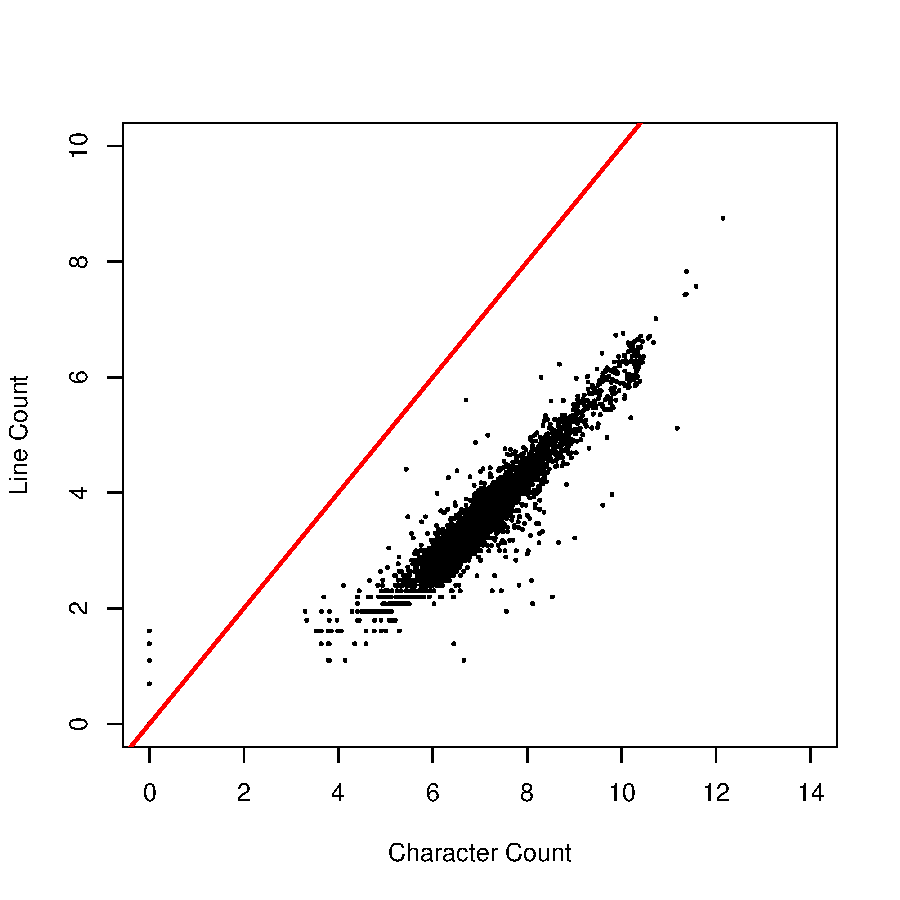
\epsfig{file=Spam/CharVSLineCount,width=10cm}
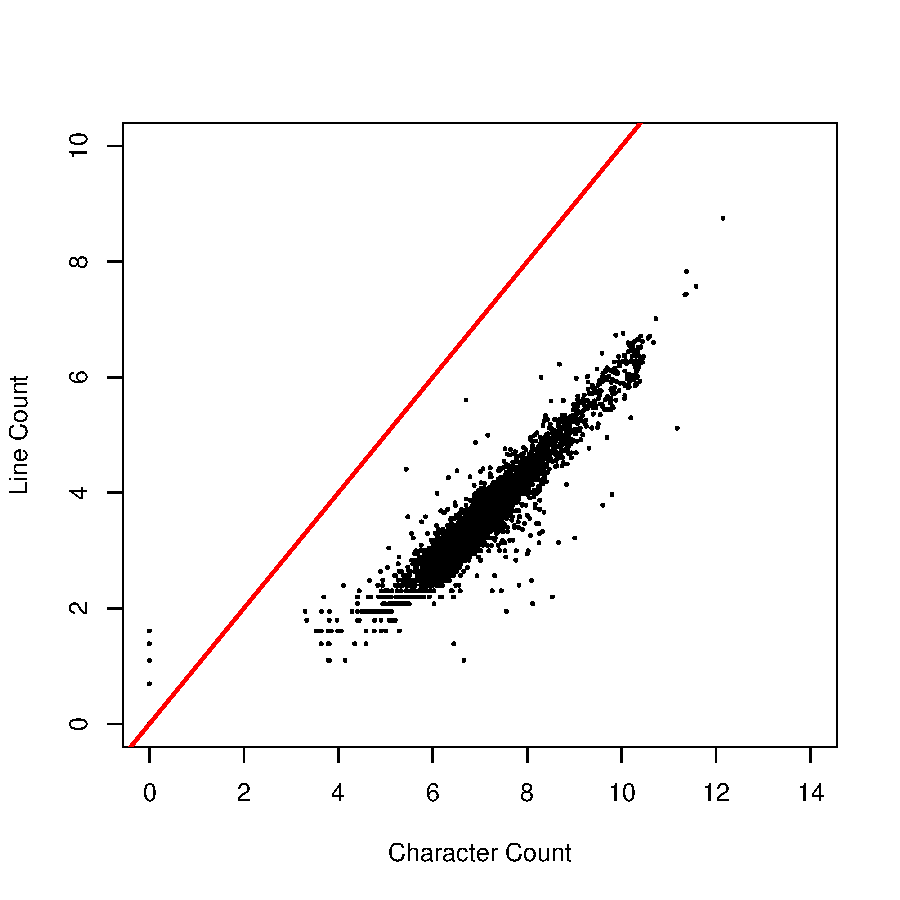
\includegraphics[width=10cm]{Spam/CharVSLineCount.pdf}
\caption{A scatter plot of the number of lines in the 
body of an email message against the number of characters
in the body.  Note that the plot is on log scale, and $1$
is added to all of the values before taking logs.
A few email messages have a few blank lines and nothing
else. These are the only points that fall above the 
$y = x$ red line.}
\label{fig:compareCharLines}
\end{figure}


\subsection{Exploratory Data Analysis}

We derived a few dozen variables from the header, body, and
attachments of each email message. 
Before conducting a formal analysis, we may ask ourselves,
whether or not these derived variables are useful
for predicting spam.
Before embarking on a complex statistical analysis it is
often a good idea to perform some simple analyses to get
a better understanding of the data and its possibilities.
This exploratory analysis may indicate that we need to
do a better job of determing variables from the messages.
This will not only help us in our future statistical
analysis, it will also help us check that the variables
have been correctly coded.

We explore the percentage of capitals in the message body, 
comparing this percentage among spam versus ham messages.  
Side-by-side boxplots (Figure~\ref{fig:boxplotSpam}) help 
us compare the distributions for these two groups.
We see from the boxplots that about 75\% of the ham
data have values at about the lower quartile for the spam
values even though the ham group maximum is much larger
than the spam maximum.  Putting the boxplots on a log
scale makes it easier to make this comparison.
Another way to see this is with a quantile-quantile 
plot. If the two distributions are roughly the same shape
then their paired quantiles will fall on a line.
We see that this is the case for the percent capitals
with spam having a larger mean and greater spread than ham. 
(A slope other than 1 indicates the distributions have
different spread, and an intercept other than zero indicates
a shift in the distributions).

\begin{verbatim}
boxplot(percentCapitals ~ isSpam)
boxplot(log(percentCapitals) ~isSpam)

qqplot(log(percentCapitals[isSpam]),
       log(percentCapitals[!isSpam]))

summary(bodyCharacterCount[isSpam])    
 Min. 1st Qu.  Median    Mean 3rd Qu.    Max.
   0     593    1459    3171    3735   71450

summary(bodyCharacterCount[!isSpam])
 Min. 1st Qu.  Median    Mean 3rd Qu.    Max.
   0     441     883    2290    1567  188500
\end{verbatim}

\begin{figure}
%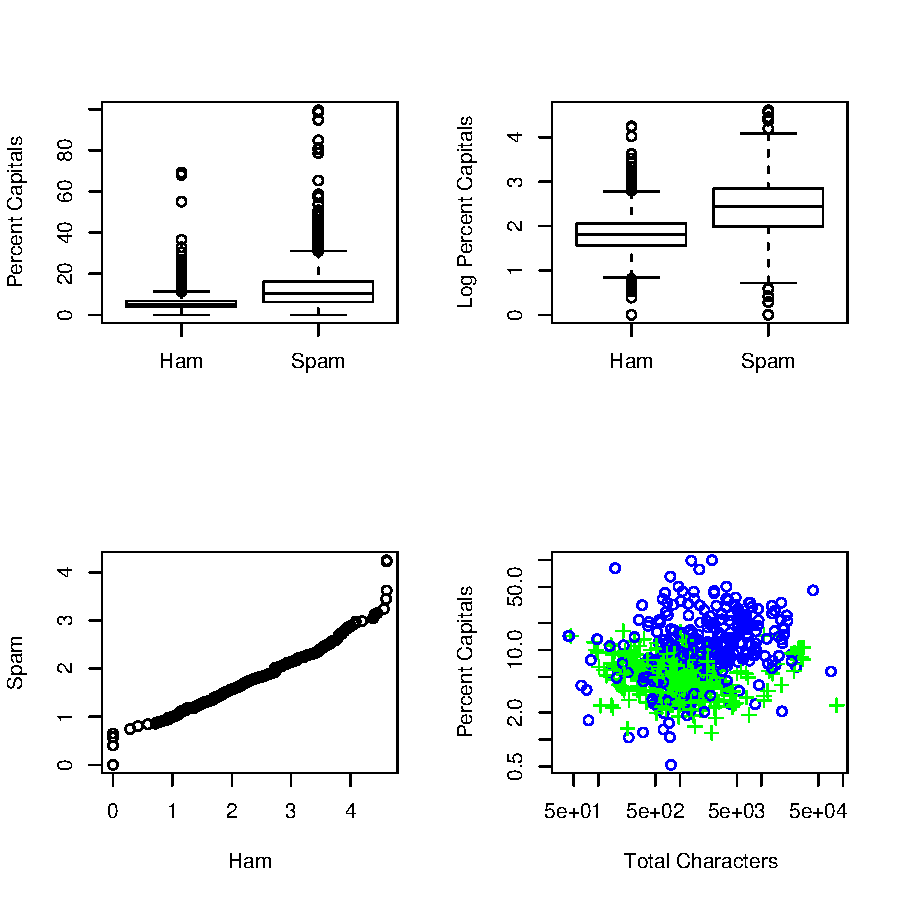
\epsfig{file=Spam/EDApercentCapitals}
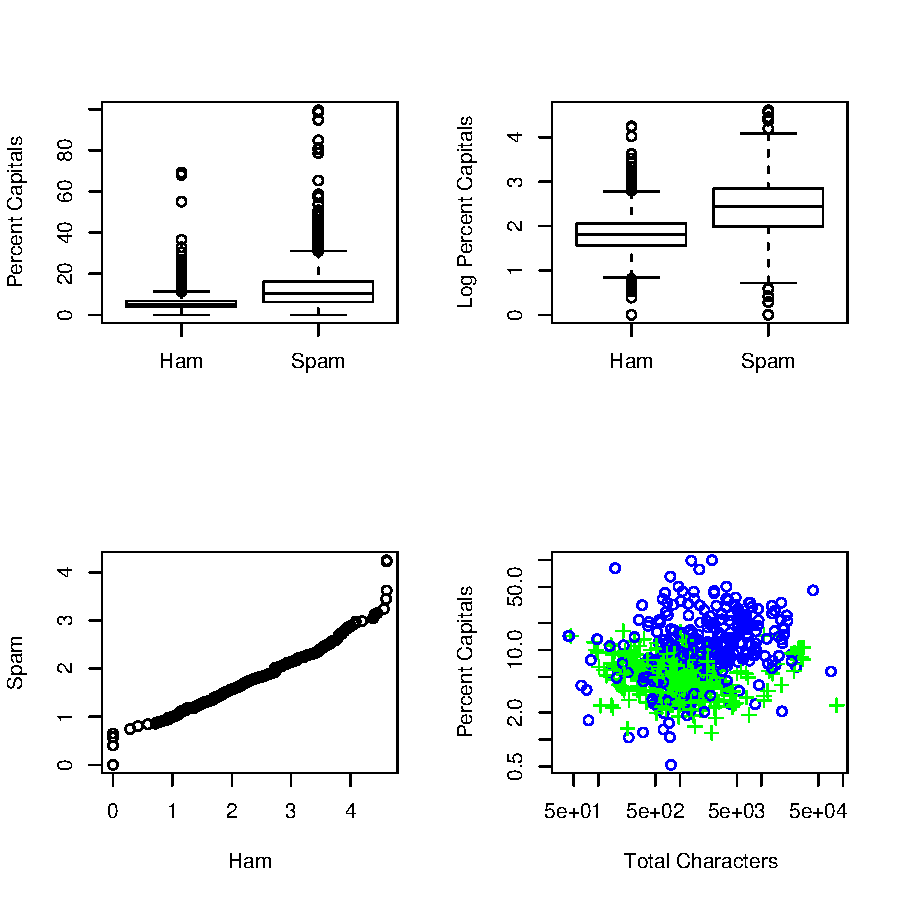
\includegraphics{Spam/EDApercentCapitals.pdf}
\caption{In the two sets of boxplots (top) we see that the 
distribution of the percentage of capitals is skewed with a 
long right tail. 
On a log scale, it is easier to see that about $3/4$ of the spam 
have more capital letters than most of the ham. 
The quantile plot (bottom left) shows that the distribution of capitals
is roughly the same shape for ham and spam.
In the lower right plot, we compare two variables,
percent capitals (crosses) and number of characters (circles)
for 800 randomly sampled emails.}
\label{fig:boxplotSpam}
\end{figure}

Further, we can compare the joint distribution of 
the percentage capitals and the number of characters 
in the body of the message via a scatter plot, 
where the ham is denoted by crosses and the spam by circles.
We see a lot of overlap between ham and spam but the spam
messages tend to be longer and have a greater percentage of capitals.

The numerical summary of the number of attachments (below)
shows that there is very little difference between
spam and ham in that most messages have no attachments.
It is doubtful that this variable will be useful
for classification.
In the two mosaic plots in Figure~\ref{fig:mosiacRe} 
we see that the spam messages are less likely to contain 
an ``Re'' than ham, but more likely to have a numeric end 
to the email address.

\begin{verbatim}
> summary(numAttachments[isSpam])
      Min. 1st Qu.  Median    Mean 3rd Qu.    Max.
    0.0000  0.0000  0.0000  0.2658  0.0000  6.0000
     summary(numAttachments[!isSpam])
     Min.  1st Qu.   Median     Mean  3rd Qu.     Max.
    0.00000  0.00000  0.00000  0.09704  0.00000 19.00000

> par(mfrow=c(1,2))
> mosaicplot(table(isSpam, isRe),shade = TRUE)
> mosaicplot(table(isSpam, fromNumericEnd),shade = TRUE)
\end{verbatim}

\begin{figure}
%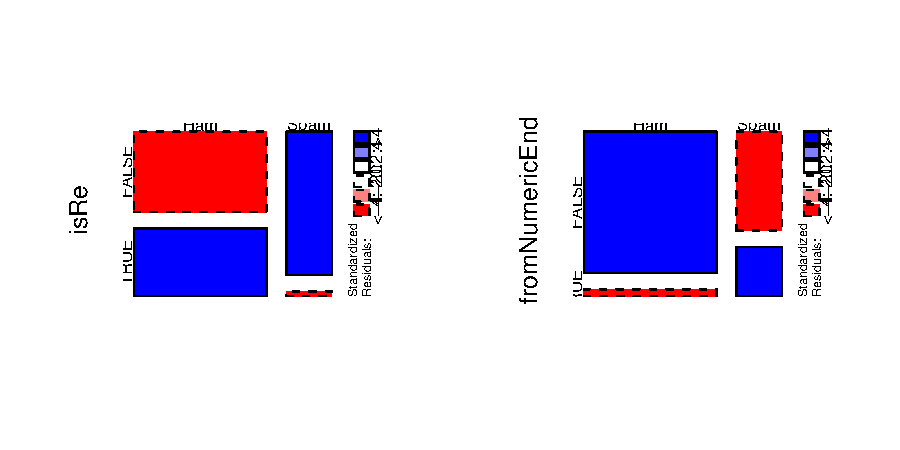
\epsfig{file=Spam/EDAmosaic}
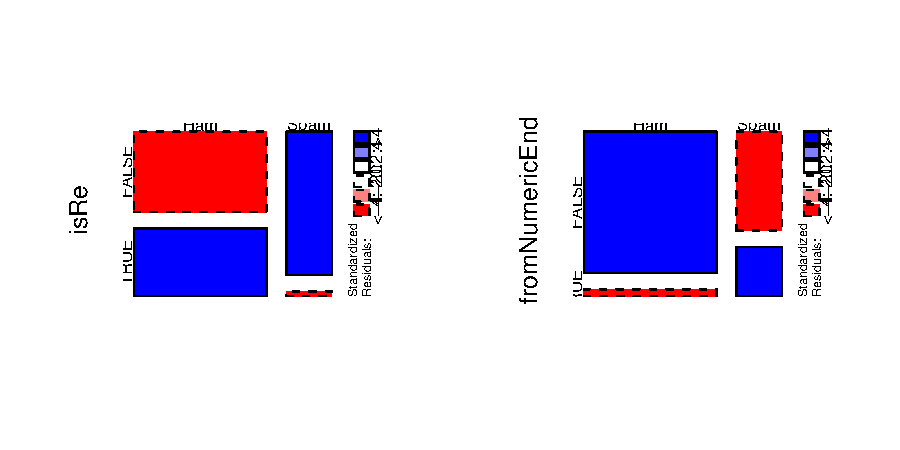
\includegraphics{Spam/EDAmosaic.pdf}
\caption{These two mosaic plots use area to denote 
the proportion of messages that fall in each category.
The plot on the left shows that most of the messages
are ham and have no Re in the subject line.
}
\label{fig:mosiacRe}
\end{figure}


\subsection{Nearest neighbor and Cross-validation algorithms}
Our goal is to create a nearest neighbor classifier to predict whether
a mail message is spam or ham.  To classify an email message, we work
with the variables derived (Section~\ref{sec:derivedVar}) from a
message to find its $k$ nearest neighbors and use them to classify the
message.  A simple classification can be made according to whether the
majority of the $k$ neighbors are spam or ham.  But, we need to
determine $k$.  At one extreme, we have nearest neighbor
classification, when $k$ is $1$, and the new email is classified as
spam or ham depending on whether its nearest neighbor is spam or ham,
respectively.  At the other extreme, we could use all the data
available to us to classify the new email. In this case, the
classification would be the same for any email, i.e. it would be ham
if the majority of the emails in the training set are ham.

To choose a value for $k$, we compare how well the method does for
messages where we know the truth, i.e. when we know whether the new
email is spam or ham.  We can compute the probability that a mistake
is made.  As with the Naive Bayes method in
Section~\ref{sec:naiveBayes}, there are two types of mistakes: a Type
I error occurs when a ham message is incorrectly classified as spam,
and a Type II error when a spam message is misclassified as ham.  We
compare the performance of the $k^{th}$-nearest neighbor classifier
for various values of $k$ via cross-validation to determine the $k$
which best controls these errors.

In the current scenario, we think of our data as pairs $(x_i, y_i)$
for $i= 1, \ldots , n$, where $x_i$ represents the vector of values
for the derived variables from the $i^{th}$ electronic-mail message,
and $y_i$ is an indicator for spam, i.e. it is $1$ when the message is
spam and 0 otherwise.  When a new message comes along we want to use
our nearest neighbor method along with our data to predict whether the
message is spam or ham.  For the new message, we observe the derived
variables, which we call $x_0$, and classify the message as spam if
the majority of its $k$ nearest neighbors among the $\{x_i\}$ are
spam.  For a loss function, ${l}$, the average loss will be

$$  \textbf{E} [ {l}(y_0 , h_k(x_0 ~| ~(x_i , y_i)~ i=1, \ldots , n) )],$$
where $h_k( \cdot ~| ~(x_i , y_i)~ i=1, \ldots , n)$ represents the
nearest-neighbor method that finds the $k$ closest neighbors to $x_0$
among the $x_i$ that are closest to $x_0$ and returns 1 (spam) or 0
(ham) according to whether the corresponding $y_i$ are a majority of
1s or 0s, respectively (Figure~\ref{fig:knnDiagram}).  Zero-one loss,
depending on whether $y_0$ is spam or ham, gives us the desired Type I
and II errors.  As with the Naive Bayes method, we use $v$-fold
cross-validation to approximate this expectation and find the
minimizing $k$.  That is, we divide at random the original data into
$v$ subsets of roughly equal size.  These subsets, $P_1$, $P_2$ ,
$\ldots$, $P_v$ form a random partition of the data.  Then for each
subset, $P_i$, we use $P_i^c$ as the training set:

$$ \frac {1}{v} \sum_{i=1}^v \frac {1} {\#P_i} \sum_{x_j \in P_i} {l}(y_j , h_k(x_j ~|~(x,y) \in P_i^c )) $$
Note that we treat the observations in $P_i$ as new observations and
look for neighbors to these new observations among those in $P_i^c$.
To estimate Type I error we take the average of those $(x_j , y_j)$ in
$P_i$ where $y_j = 0$, and similarly we restrict the average to those
$y_j = 1$ to estimate Type II error.

\begin{figure}

\vspace{2in}

\caption{Diagram of red and green nearest neighbors 
from his lecture notes.}
\label{fig:knnDiagram}
\end{figure}

The above equation helps us understand how cross-validation is
applied to the case of nearest neighbor estimation. It also suggests 
a way to code the nearest neighbor and cross-validation procedures:

\begin{itemize}
\item Partition the data into $v$ subsets.
\item For each observation in a partition $P_i$, 
find the k nearest neighbors in $P_i^c$.
\item Classify the observation according to its neighbors' values. 
\item Repeat for $k = 1, \ldots ,\#P_i^c$
and for $i = 1, \ldots ,v$. 
\end{itemize}

To find the $k$ nearest neighbors, we need to find the distances
between observations. The \Sfunc{dist} function takes a data
frame and computes the distance between all pairs of rows in the data
frame. (For now we ignore the issue of which metric to use and proceed
with the default Euclidean distance).  Although the equation above
provides an intuitive explanation of cross-validation for this
example, it does not indicate an efficient way to program the method.
In this case study, many unnecessary computations can be avoided with
a little attention to the specifics of the problem.  Two important
ones are described here:

\begin{itemize}
\item To find the nearest neighbor in the training set to an
  observation in the validation set, we need to find the distance from
  the validation observation to all observations in the training set.
  But once we have computed all of these distances then we also have
  the $k$ nearest neighbors for $k = 2, \ldots , \#P_i^c$.

\item In one iteration of cross-validation, we need to find the
  distances between all observations in $P_i$ and all those in $P_i^c$
  (Figure~\ref{fig:knnCVdiagram}).  When we consider the iteration
  over $i$, we notice that we need to find distances between all pairs
  of observations because each observation belongs to one validation
  set and $v-1$ training sets.  So, we need only compute all distances
  between pairs of observations in the data once and pull out those
  that are needed for a particular fold $i$ in the $v$-fold
  cross-validation method.
\end{itemize}

\begin{figure}
\vspace{2in}
\caption{Grid figure for cross validating distance matrix}
\label{fig:knnCVdiagram}
\end{figure}

These two properties point out an important feature of 
nearest neighbor methods: no models or parameters are fitted  
that reduce the dimensionality of the problem.
That is, all of the training data must be held around in
order to compute the distance of a new observation to past
observations. 
As a result, for efficiency in terms of space and time,
it is important to take these properties into consideration
when developing the code.
When we do, we see that once we compute all pairs of distances 
between observations, then reordering and subsetting gives us 
all the cross-validated nearest neighbors for any (all) $k$.

The following functions, \SFunctionRef{knnCV} and
\SFunctionRef{knnPredict} take these aspects into consideration.  The
\SFunctionRef{knnPredict} function makes predictions for a test set.
Its inputs are: an $m \times n$ matrix of distances between $m$
observations in the validation and $n$ observations in the training
set; the true classifications for the training set, where spam is
\SValue{TRUE} and ham \SValue{FALSE}; and additional parameters to
specify how to handle ties in voting.  The output is an $m \times p$
matrix of logicals indicating the classification of each element in
the validation set for $p$ different $k$ between \SVariable{kmin} and
\SVariable{kmax}.

The function \SFunctionRef{knnCV} finds the cross-validated prediction
error.  The inputs of this function are: an $N \times N$ matrix of
distances between $N$ observations, the true classification of each of
the $N$ observations, and an $n \times v$ matrix of indices from $1,
..., N$, where the $j^{th}$ column contains the indices $(i_1, \ldots,
i_n) \in \{1, \ldots , N\}$ of the observations in the $j^{th}$
validation set.

\begin{verbatim}
knnCV <-
function(Dist, actualClass, groups, kmin = 1, kmax = 100)
{
# Determine which k's will be reported
  krange  = range(c(kmin, kmax))
  krange[2] = min(krange[2], nrow(groups))  
  knnCorrect = matrix(0, nrow = 0, 
                      ncol = (krange[2] - krange[1] + 1))

 # Loop over v to make predictions for the v test sets
 # using the corresponding v training sets.

  for (i in 1:ncol(groups)) {
    knnPreds = knnPredict( Dist[groups[,i] , - groups[,i]],
                           actualClass[ - groups[, i]], 
                           krange[1], krange[2])

# Determine if the predictions are correct
    knnCorrect = rbind(knnCorrect, 
                   knnCheck( knnPreds, 
                             actualClass[groups[, i]]))
  }

# Compute the Type I and II errors
  ans = predError(knnCorrect, actualClass[groups])
  ans
}
\end{verbatim}

\begin{verbatim}
knnPredict <-
function(distM, trainClass, kmin, kmax, tieRandom = FALSE, 
         tieNearest = FALSE)
{
# distM: m by n matrix where we have m test and 
# n training observations
# trainClass: vector of n logicals

# Returns m by kmax-kmin+1 matrix of logicals (predictions)
  votes <-
      apply(distM, 1, function(nn) {
               tmp = trainClass[order(nn)[1:kmax]]
               percents = cumsum(tmp)/(1:kmax)
               predict = (percents[kmin:kmax] >= .5)
               if (tieRandom) {
                 predict[percents == .5] = 
                    rbinom(n=1,size=1, prob=0.5)
               } else {
                 if  (tieNearest) {
                   predict[percents == .5] = 
                      (percents[1] > 0.5)
                 } else {
                   predict[percents == .5] = 
                      predict[(which(percents == .5) - 1)]
                 }
               } 
               predict  
               })
  t(votes)
}
\end{verbatim}

The computation of the type I and II errors follows the same
approach as shown for the Naive Bayes method so it is not
presented here.


\subsection{Cross-validating the metric}
Now that we have the ability to find type I and type II 
errors for various values of $k$, we turn to the problem
of choosing an appropriate metric for computing distances
between email messages.
One well known metric is Euclidean distance, which 
may not be appropriate for logical variables.
A binary metric may be more appropriate because logicals
take on only two possible values.  
For variables, such as the number of lines in the
body of the email \SVariable{numLinesInBody}, 
the percentage of capital letters in the subject of the email
\SVariable{percentCapitals}, 
and the number of recipients \SVariable{numRecipients},
we compute the Euclidean distance between two email
messages $i$ and $j$ as follows:
\begin{eqnarray*}
 [(numLinesInBody_i &-& numLinesInBody_j)^2 \\
   &+& (percentCapitals_i - percentCapitals_j)^2\\
     &+& (numRecipients_i - numRecipients_j)^2 ]^{1/2} 
\end{eqnarray*}
and the Manhattan distance between them is:
\begin{eqnarray*}
  |numLinesInBody_i &-& numLinesInBody_j|\\
    &+& |percentCapitals_i - percentCapitals_j|\\
      &+& |numRecipients_i - numRecipients_j|
\end{eqnarray*}

Note however that the percentage of capitals in the subject will always
be between 0 and 100, whereas the number of lines in the body of an
email can get quite large.
We may want to normalize the continuous variables before
computing the distance between two records.
One way to do this is center the variable on
the mean value and to scale it by the standard deviation,
i.e.
$$
\frac{(numLinesInBody - mean(numLinesInBody))}
{SD(numLinesInBody)} .$$
Alternatively, the median and median asolute deviation could
standardize a variable.
Or, proportions and percentages (scaled by 100) could be left
alone, and the other non-binary values scaled by 3SDs to bring
them all in the range of 0 to 1. 
The Canberra distance includes a standardization,
\begin{eqnarray*}
 &~& \frac {|numLinesInBody_i - numLinesInBody_j|} 
  {|numLinesInBody_i + numLinesInBody_j|} \\
    &+& \frac {|percentCapitals_i - percentCapitals_j|} 
            {|percentCapitals_i + percentCapitals_j|} \\
      &+& \frac {|numRecipients_i - numRecipients_j|} 
            {|numRecipients_i + numRecipients_j|}
\end{eqnarray*}

The rule for the asymmetric distance is as follows:
compute the number of elements in the vectors for which at least one
of the two records has a non-zero value; count the number of these
elements for which the two records are different (i.e. one is a 1
and the other is a 0); and report the proportion of these two
counts as the distance.  
When neither record has any 1s, the distance is 0.
An example may help. Suppose we look the three variables
\SVariable{isRe}, \SVariable{replyUnderline} and \SVariable{multipartText}
and we have email records $i$ and $j$ as

\begin{verbatim}
    isRe    replyUnderline   multipartText
    TRUE          FALSE         FALSE
    FALSE         FALSE         FALSE
\end{verbatim}
The distance is 1 (or 1/1) since there is only one
entry for which there is at least one 1 (i.e. TRUE).
And in this position (the first), the values are different so we count 1.
For two records of the form
\begin{verbatim}
     isRe    replyUnderline   multipartText
     TRUE        TRUE            TRUE
     FALSE       FALSE           TRUE
\end{verbatim}
the distance would be 2/3.

Whichever metric we use, we then have to combine the distance 
values, $D$, for the binary and non-binary variables. 
An obvious way to combine them is
\[ D_{\textrm{non-binary}} + w D_{\textrm{binary}}\]
Of course, we need to determine $w$, so we use cross-validation
to obtain values for both $w$ and $k$.

Since we have our cross-validation functions for finding $k$, 
we can write a simple wrapper function to cross-validate the metric
and the weight $w$.
The function \Sfunc{knnExpr} takes various values of these
three parameters ($k$, $w$, and the metric) and cross-validates the
prediction error for all combinations of the values.  
The R function
\Sfunc{dist} computes distances via various metrics,
including Euclidean, Manhattan, Minkowski, Canberra, 
and asymmetric binary.

\begin{verbatim}
knnExpt <-
function(derivedEmails, actualClass, w = 1, 
         metric = c("euclidean", "manhattan", "canberra"), v = 10, 
                    perm = sample(1:nrow(derivedEmails)),
                    kmin = 1, kmax = 100)
{
   logVars = which(sapply(derivedEmails, is.logical))
   conVars = (1:ncol(derivedEmails))[-logVars]

   binDist = as.matrix(dist(derivedEmails[, logVars], 
                            method = "binary"))
   groups = cvSet(v = v, perm = perm) 

   for(i in metric) {
      conDist = as.matrix(dist(derivedEmails[, conVars],
                               method= i))
      predErrs = list()
      for (j in 1:length(w)) 
        {
           Dist = (w[j] * binDist) + conDist
           predErrs[[j]] = knnCV(Dist, actualClass,   
                                 groups, kmin, kmax)
           remove(Dist)
        }
      assign(paste("outKNN", i, sep = "."), predErrors)
      save(paste("outKNN", i, sep = "."), 
           file =paste("outKNN", i, ".rda", sep = ""))
    }
}
\end{verbatim}
Note that we use the \Sfunc{assign} function here 
in order to create an R object with name based on the metric
specified via an input parameter at the time the function is called. 

We use the following script to analyzes the email messages.
It takes the default values for the metrics (Canberra, Manhattan,
and Euclidean) and for the $k$ (1 to 100), and specifies $w$ only.
We may want to run the script in batch mode (say more ...).
The script is annotated to explain the various steps of the 
analysis process.

\begin{verbatim}
# All of the functions are in the file myKNN.S.
source("myKNN.S")
# Load the data to cross-validate
load("knnData.rda")

# After exploratory data analysis we settle on transforming
# the non-binary variables which are also not proportions/percentages

logTrans = c("numLinesInBody", "numAttachments", 
             "numRecipients", "numDollarSigns", 
             "bodyCharacterCount", "subjectQuestCount",
             "subjectExclamationCount", "averageWordLength")

for (i in logTrans) {
    derivedEmails[, i ] = log(1+ derivedEmails[, i])
}
# Transform the time to fall between 0 and 1.
derivedEmails[,"hourSent"]= derivedEmails[,"hourSent"]/24

actualClass = derivedEmails[, "isSpam"]
knnExpt(derivedEmails, actualClass, w = c(1,5,10,15,20))
\end{verbatim}

Once we have the cross-validated prediction errors, plots such as those
in Figure~\ref{fig:knn1to100} show us that the metrics produce similar
results, with Manhattan and Canberra slightly outperforming Euclidean.
We make the following observations.

\begin{figure}
%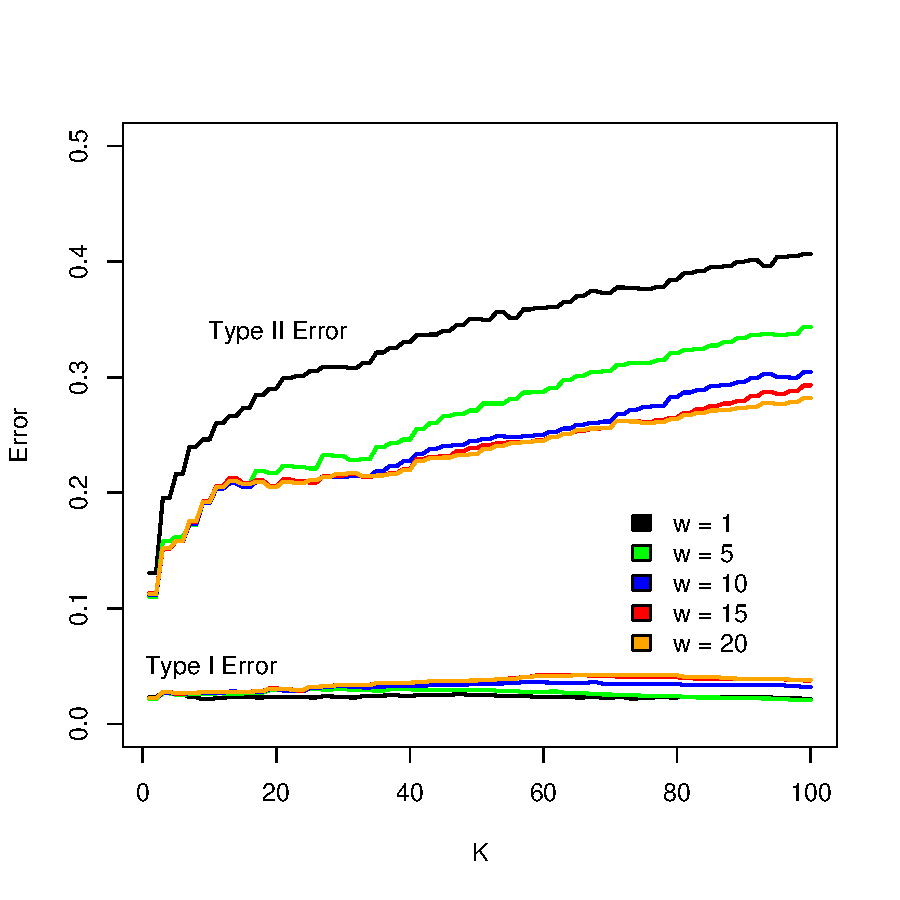
\epsfig{file=Spam/knn1to100}
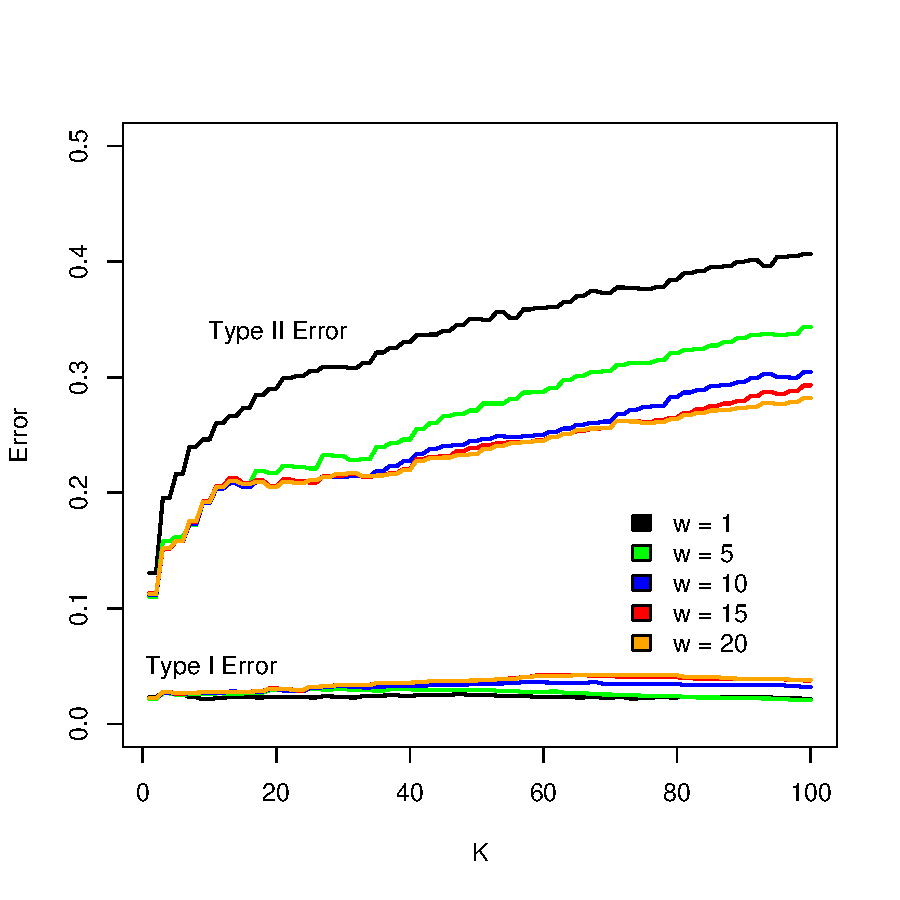
\includegraphics{Spam/knn1to100.pdf}
\caption{Type I and II error rates for Canberra distance.}
\label{fig:knn1to100}
\end{figure}

\begin{itemize}
\item The Type I error is much smaller than Type II, and has less variability.

\item There is a sharp increase in Type II errors as $k$ grows, and we need to
zoom in on the region where $k< 15$ in order to see better which value of 
$w$ should be used (Figure~\ref{fig:knn1to15}).

\begin{figure}
%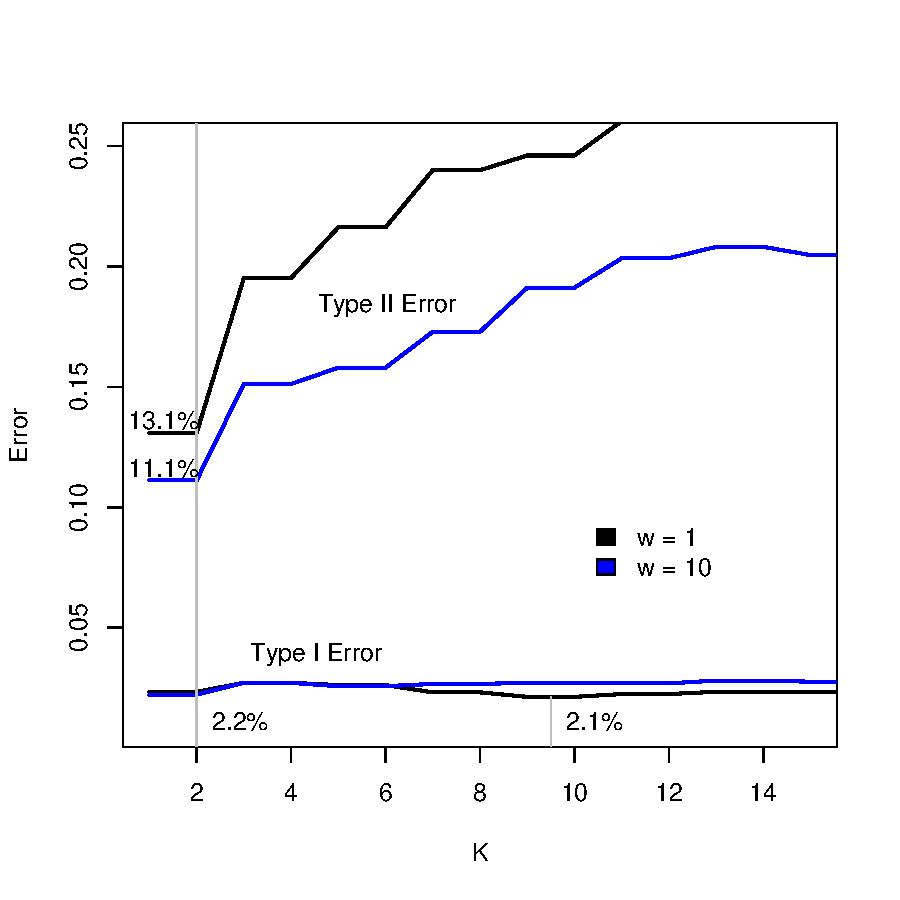
\epsfig{file=Spam/knn1to15}
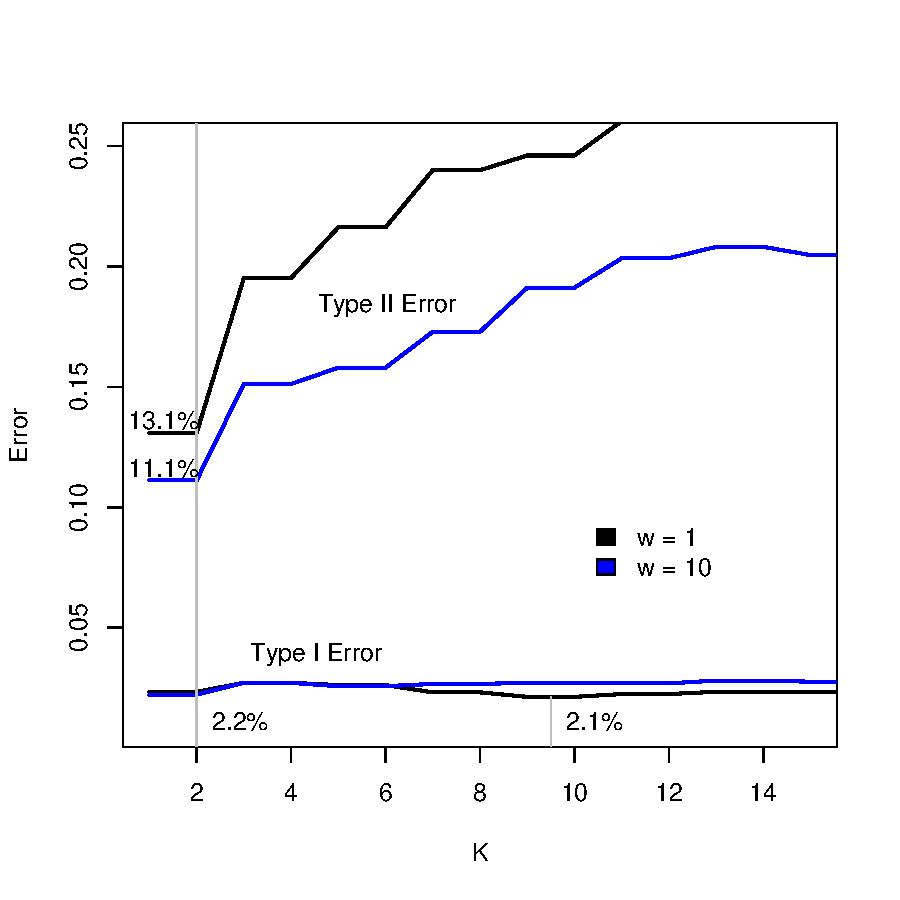
\includegraphics{Spam/knn1to15.pdf}
\caption{Type I and II error rates for Canberra distance.}
\label{fig:knn1to15}
\end{figure}

\item The Type II error is minimized at $k=1, 2$, regardless of the value for $w$,
but it does appear that there is a big drop in the Type II errors for larger weights.
In order to see which weights do best, we need to zoom in on the Type II errors 
separately because they are on a different scale in comparison to Type I errors
(Figure~\ref{fig:knnTypeII}).
In this figure, we see that the curves for Type II error
are the same shape with w=10 being the best.

\item Similarly, we see that for Type I (Figure~\ref{fig:knnTypeI}), 
when $w=1$, the best $k$ is about $9$, with $k=1,2$ a close second. 
For $w = 1$, the Type I error curve has a sharp dip at the minimum
and slowly rises for larger $k$, but remains relatively small in
comparison to the Type II error for all $w$..
\end{itemize}

Based on these considerations, we choose $k = 2$, $w = 10$, and the 
Canberra metric.

\begin{figure}
%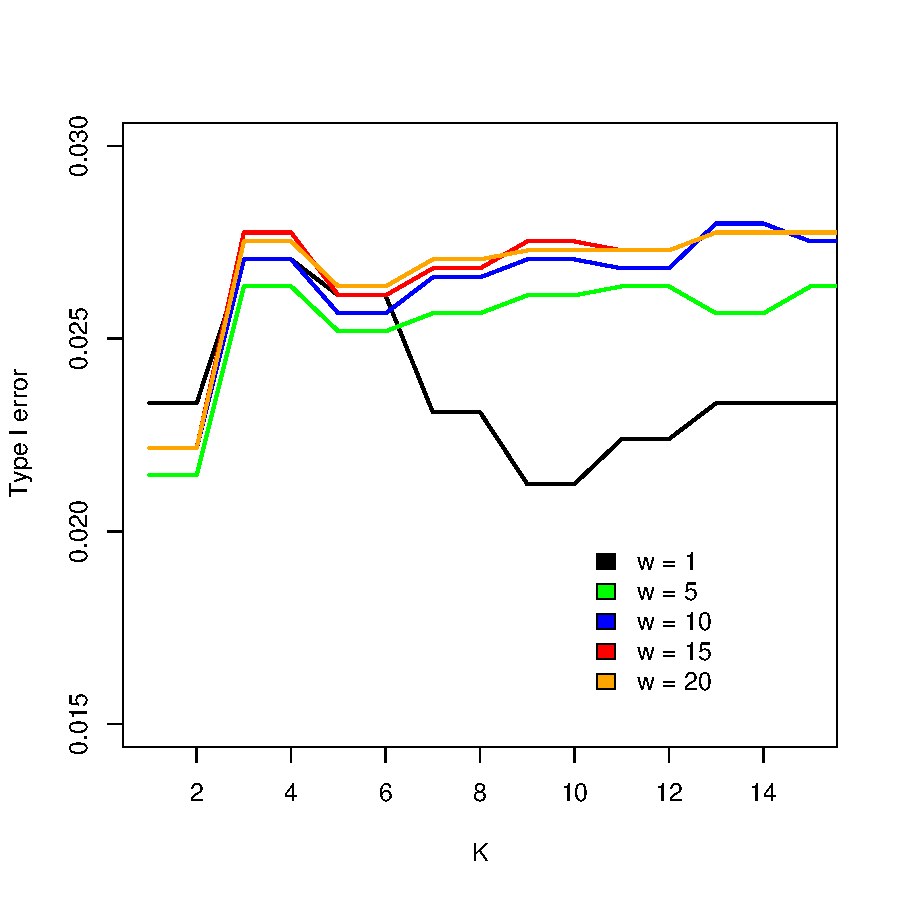
\epsfig{file=Spam/knnTypeI}
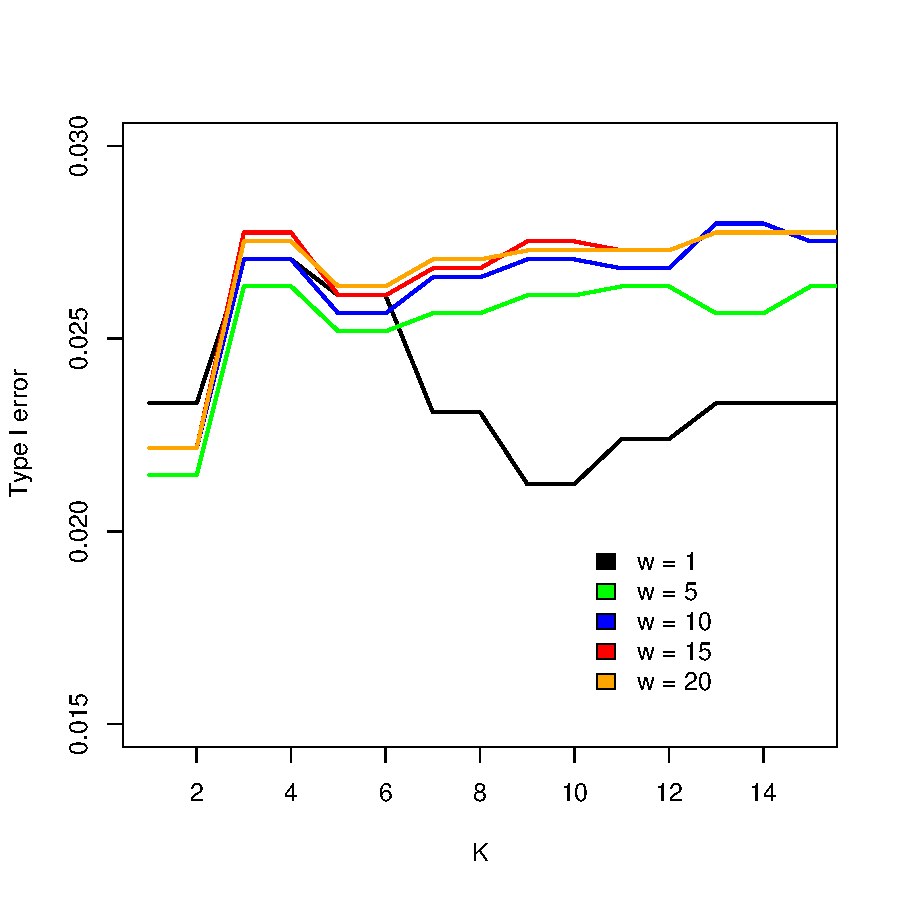
\includegraphics{Spam/knnTypeI.pdf}
\caption{Type I error rates for Canberra distance.}
\label{fig:knnTypeI}
\end{figure}

\begin{figure}
%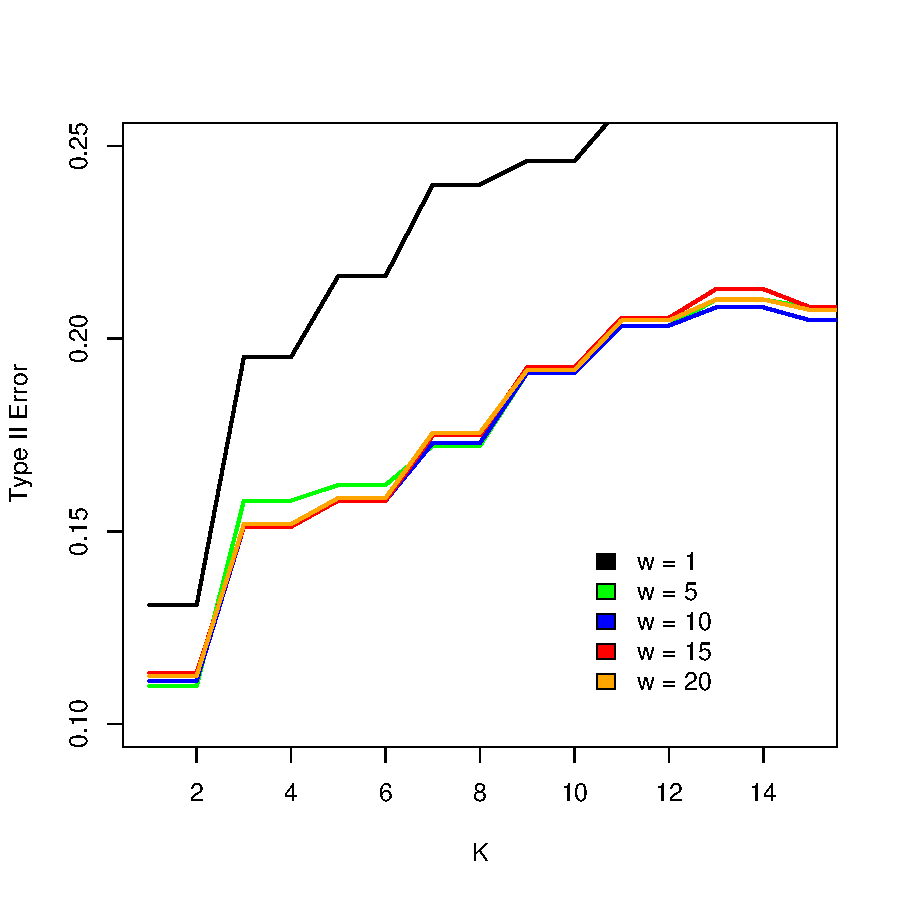
\epsfig{file=Spam/knnTypeII}
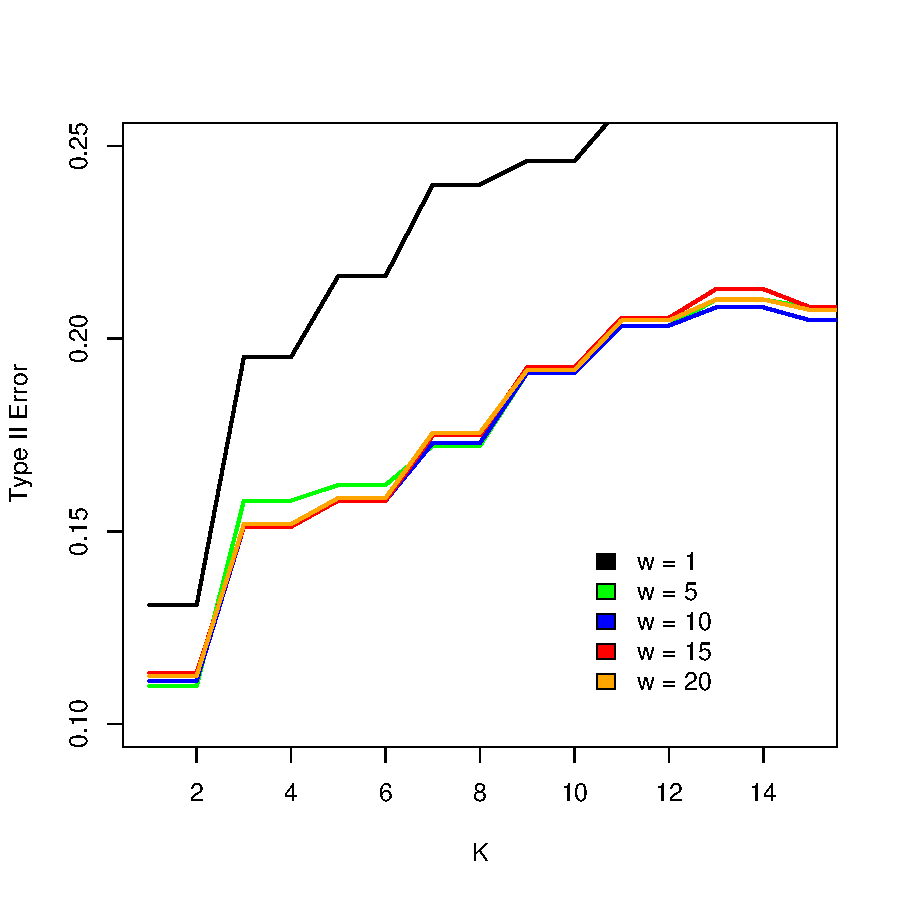
\includegraphics{Spam/knnTypeII.pdf}
\caption{Type II error rates for Canberra distance.}
\label{fig:knnTypeII}
\end{figure}


\subsection{Further validation and comparison}
We can validate how well $k^{th}$ nearest neighbor
performs on a new, independent set of date.
We mean here validate, not cross-validate, because
we have set aside a portion of the Spam Assassin data for 
this purpose, and did not use it to select
the parameters, $k$, $w$ and the non-binary metric.
We now apply the nearest-neighbor method to these
new data, with $k =2$, $w = 10$, and the Canberra metric,
and compute the Type I and II errors.

We reap the benefits now of having written separate functions
for the two distinct tasks: classification and  cross-validation.
We do not have to write additional code in order to apply
the classification to the new data.
We need only prepare the data for inputting to our function.
We first construct the distance matrix from the combined data,
i.e. the original set, \SVariable{derivedEmails} and the
new validation set of 750 messages, \SVariable{newEmails}.
Then we use \Sfunc{knnPredict} to make the
nearest neighbor predictions, where a prediction is made
for each message in \SVariable{newEmails} by looking
for neighbors among the observations in \SVariable{derivedEmails}.

\begin{verbatim}
testEmails = rbind(derivedEmails,newEmails)
nOld = nrow(derivedEmails)

binDist = as.matrix(dist(testEmails[, logVars], 
                         method = "binary"))
conDist = as.matrix(dist(testEmails[, conVars], 
                         method = "canberra"))
bothDist = (10*binDist) + conDist
remove(binDist,conDist)

actualClass = testEmails[,1]
knnPreds = knnPredict(bothDist[ -(1:nOld), 1:nOld],
              actualClass[1:nOld], kmin = 1, kmax = 10)
knnCorrect = knnCheck(knnPreds, actualClass[-(1:nOld)])
knnErrs = predError(knnCorrect, actualClass[-(1:nOld)])
\end{verbatim}

We find that both Type I and II errors are worse for these
750 new observations (they are both over 17\%).
Why did the method not work as well on these observations?
There may be a difference between the data that have been
held out and the data that we used to choose $k$ and $w$.

Exploratory analysis of the data reveals several
differences between the old and new mail messages.
These are presented in tables below.
We see that there is little difference between
the two sets of email messages in terms of the presence
of ``Dear'' in the email, \SVariable{isDear}; and
there is a small difference between old and new
as far as the amount of yelling in the subject line,
\SVariable{isYelling}. 
But there is a big difference in the use of ``Re'';
75\% of the new ham has an ``Re'', in comparison to 57\% 
of the old ham.
Also, there is a large difference when it comes to the
use of a numeric end on the email address. 
Less than 5\% of the old ham has a numeric end in comparison 
to 22\% of new ham, and roughly 30\% of spam whether old or new 
has a numeric end.

\begin{table}
\begin{tabular}{rrrrrr}
       &  &  \multicolumn{2}{c}{Old Mail} & \multicolumn{2}{c}{New Mail} \\
       & isDear & FALSE & TRUE & FALSE & TRUE \\
isSpam & FALSE & 4287  &   0  & 500 &  0\\
       & TRUE  & 1380  &  44 & 237 & 7 \\
\end{tabular}
\end{table}

\begin{table}
\begin{tabular}{rrrrrr}
       &  &  \multicolumn{2}{c}{Old Mail} & \multicolumn{2}{c}{New Mail} \\
       & isYelling & FALSE & TRUE & FALSE & TRUE \\
isSpam & FALSE & 4278  &   6  & 493 &  4\\
       & TRUE  & 1346  &  129 & 234 & 16 \\
\end{tabular}
\end{table}

\begin{table}
\begin{tabular}{rrrrrr}
       &  &  \multicolumn{2}{c}{Old Mail} & \multicolumn{2}{c}{New Mail} \\
       & isRe & FALSE & TRUE & FALSE & TRUE \\
isSpam & FALSE & 2459  & 1828 & 376 & 124\\
       & TRUE  & 1432  &  43  & 245 &  5 \\
\end{tabular}
\end{table}

\begin{table}
\begin{tabular}{rrrrrr}
       &  &  \multicolumn{2}{c}{Old Mail} & \multicolumn{2}{c}{New Mail} \\
       & fromNumericEnd & FALSE & TRUE & FALSE & TRUE \\
isSpam & FALSE & 4085  & 202  & 392  & 108 \\
       & TRUE  & 984  &  491  & 175 &  75  \\
\end{tabular}
\end{table}

The boxplots on a log scale show that: the
number of characters in the message body for the 
new ham has a long left tail (Figure~\ref{fig:knnBoxPlotBCC})
and so will more likely be confused with the old spam;
the proportion of capital letters to all letters in the
body of the message and the proportion of blanks in the 
subject line both appear about the same
in the new and old emails (Figures~\ref{fig:knnBoxPlotPC}
and~\ref{fig:knnBoxPlotPSB});
but there are far more forwards in the old ham than in
the new ham. 

\begin{figure}
%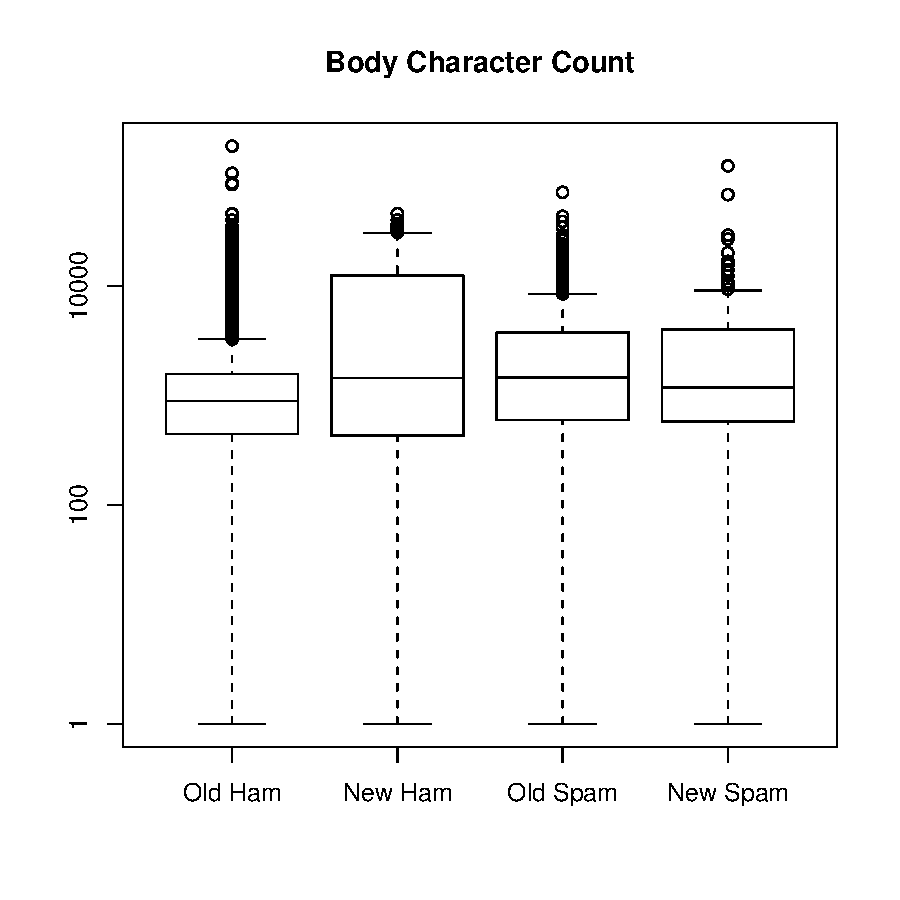
\epsfig{file=Spam/knnBoxPlotBCC}
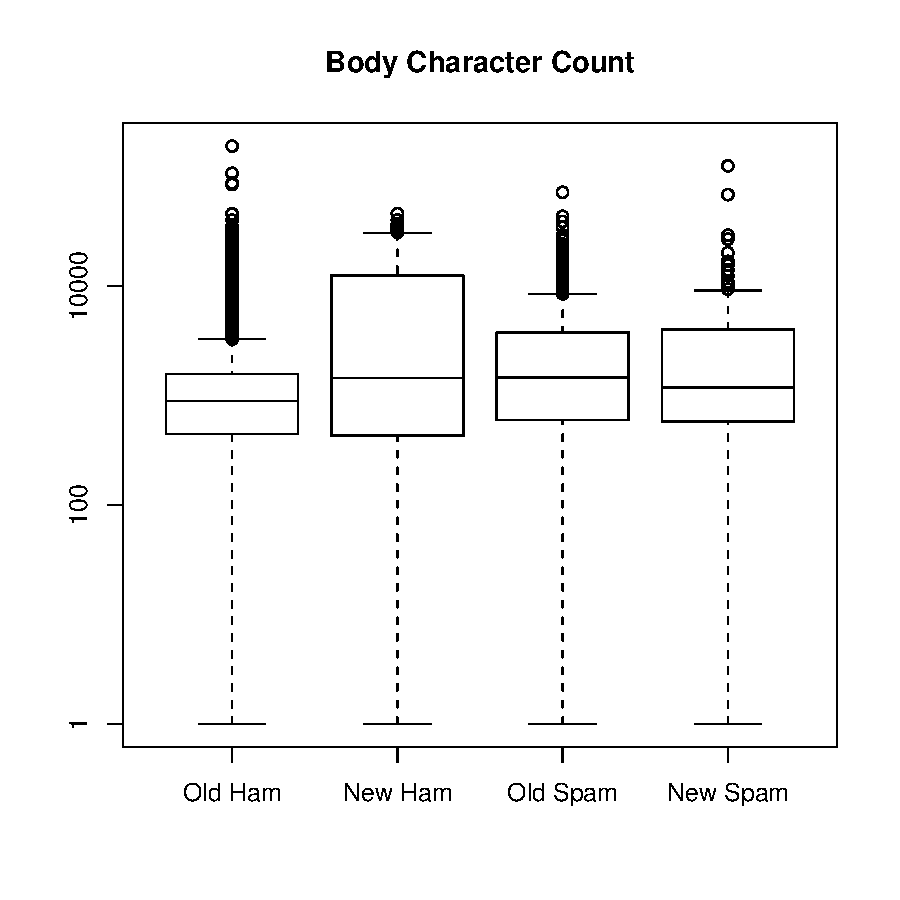
\includegraphics{Spam/knnBoxPlotBCC.pdf}
\caption{Boxplot of the number of characters in the body of the
email message. The counts are one a log scale.}
\label{fig:knnBoxPlotBCC}
\end{figure}

\begin{figure}
%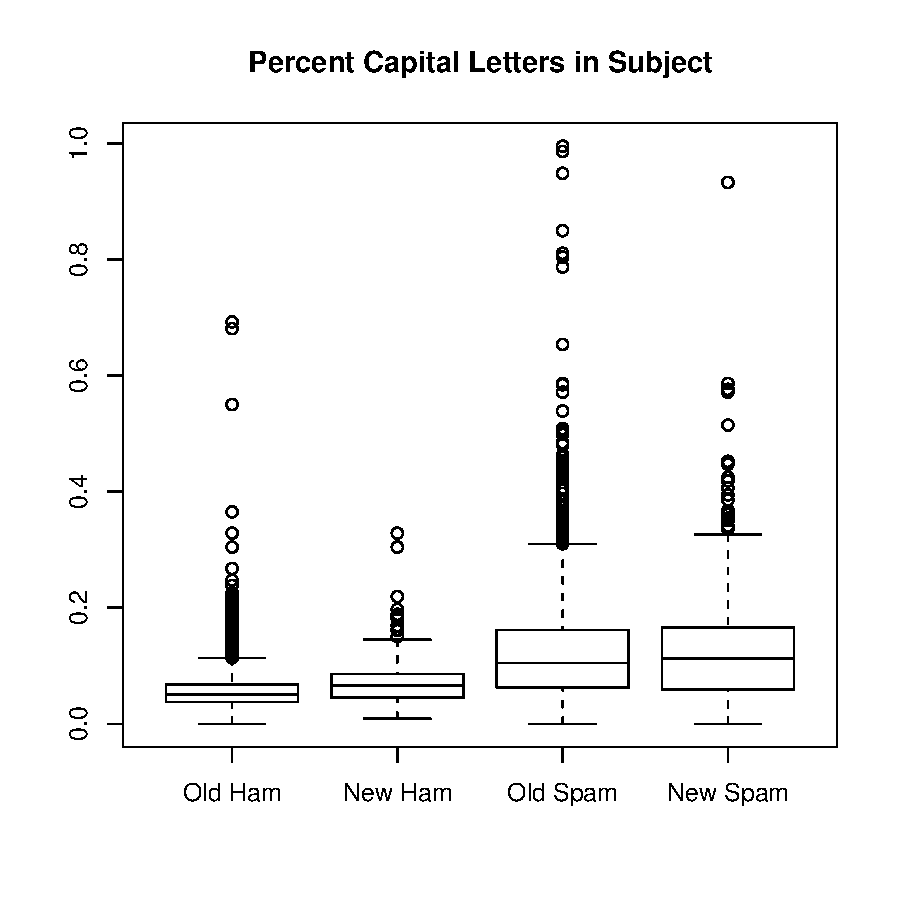
\epsfig{file=Spam/knnBoxPlotPC}
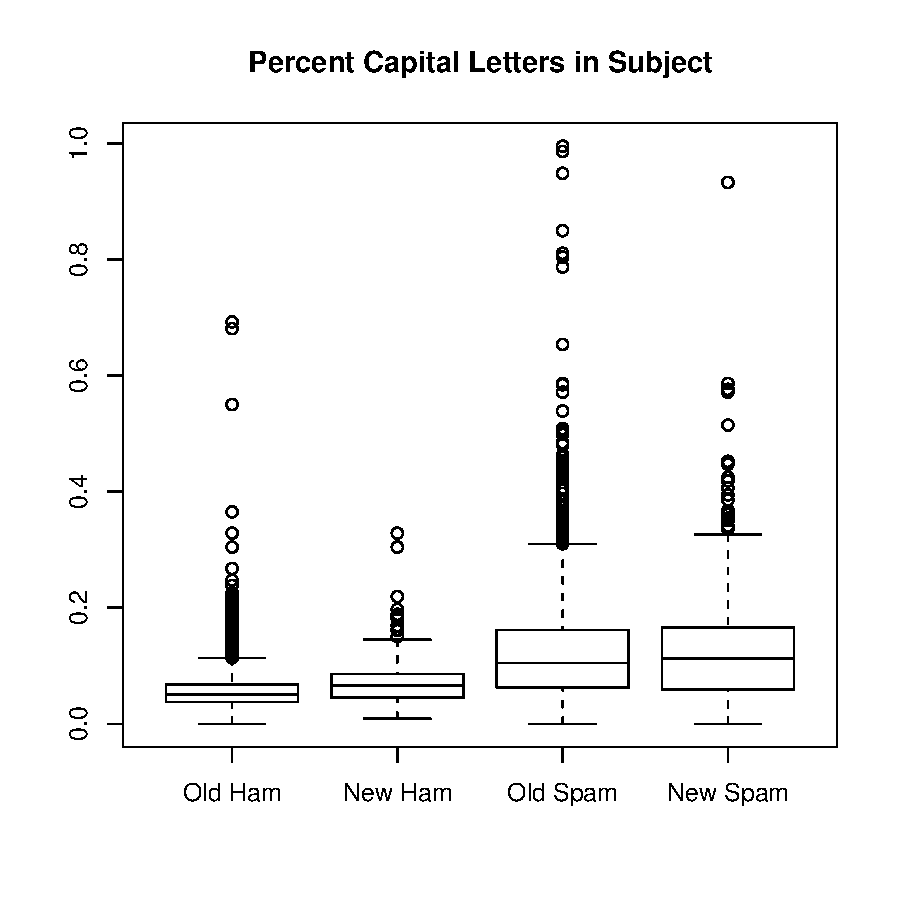
\includegraphics{Spam/knnBoxPlotPC.pdf}
\caption{Boxplot of the percenatge of characters in the body which
are capitalized. The percentage is one a log scale.}
\label{fig:knnBoxPlotPC}
\end{figure}

\begin{figure}
%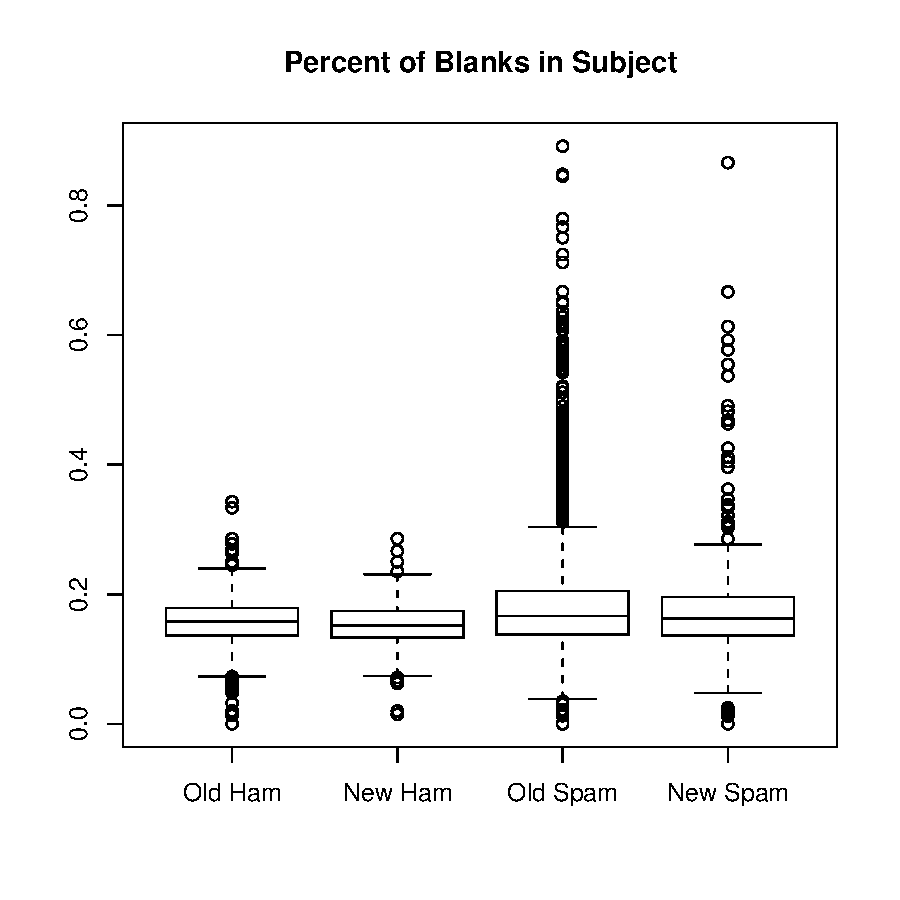
\epsfig{file=Spam/knnBoxPlotPSB}
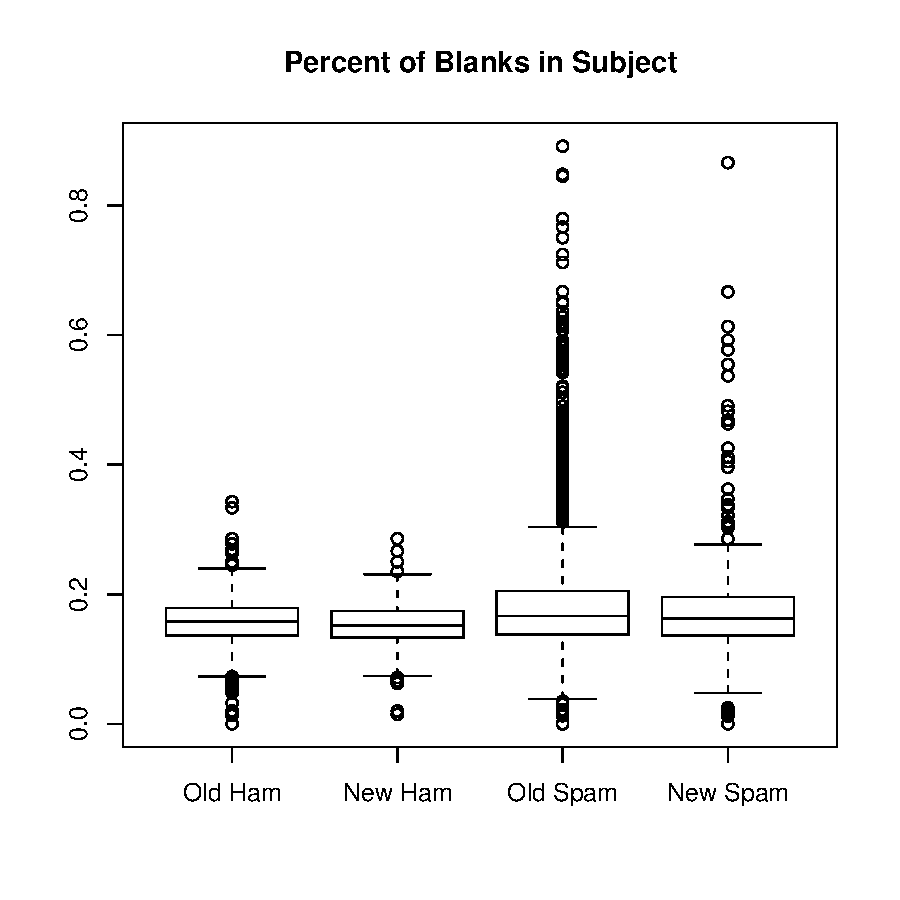
\includegraphics{Spam/knnBoxPlotPSB.pdf}
\caption{Boxplot of the percentage of blanks in the subject line.
The percentage is one a log scale.}
\label{fig:knnBoxPlotPSB}
\end{figure}


We complete the chapter by comparing our optimal nearest neighbor 
procedure to the method of classification trees.
A classification tree is an intuitively simple classification
method. Beginning at the root node of the tree, the data
split or branch into two groups according to the
value of a single variable.
For example, the first split in the classification tree shown in
Figure~\ref{fig:rpartTree} is according to the value of 
percentCapitals, where the data are divided into two groups
according to whether an observation's value for percentCapitals is
above $0.1136$ or not. 

\begin{figure}
%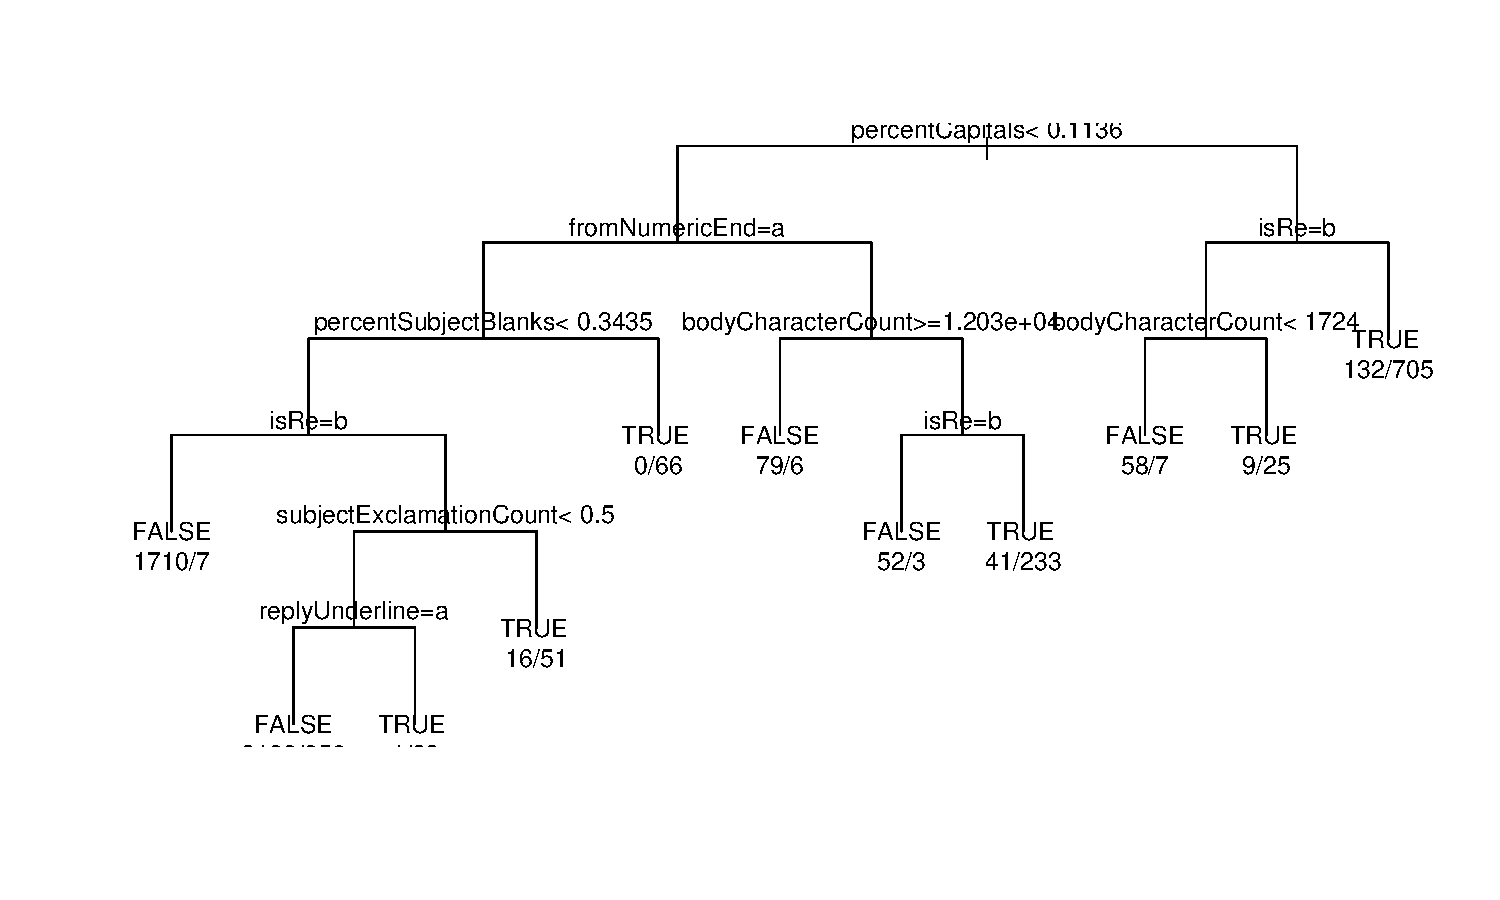
\epsfig{file=Spam/rpartTree, angle=90, height=8in}
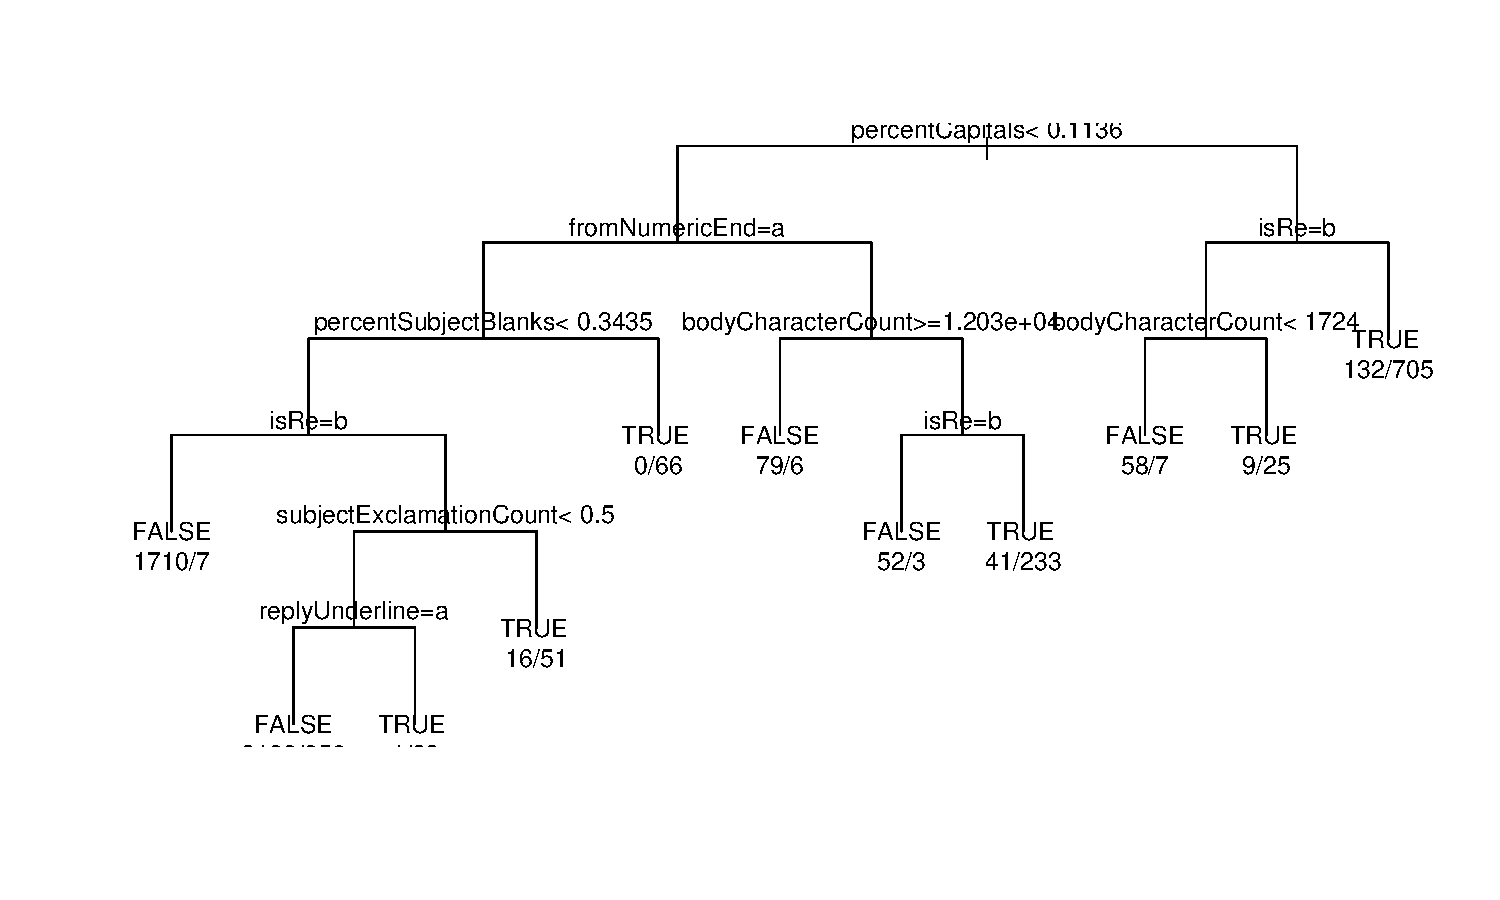
\includegraphics[height=6in, angle=90]{Spam/rpartTree.pdf}
\caption{Classification tree for spam built using the
default arguments to \Sfunc{rpart}}
\label{fig:rpartTree}
\end{figure}

Subsequent splits are made along the resulting two branches
in a similiar fashion; that is, each split considers the
value of a single variable and subdivides the 
data at that node into two groups according to whether the
observation falls above or below the chosen value. 
The variables must all be either factors or numeric.
For a factor variable, the split is made according to a 
particular level of the factor; that is, if an observation has 
that particular factor level than it branches to the right,
otherwise it branches to the left.

The branching attempts to make the observations in the resulting 
subgroups as similar as possible. 
All observations in a subgroup 
at the end of the tree (i.e. a leaf) are given the same classification.
If the observations in the leaves are as homogeneous as possible, 
then we reduce the prediction error.
Does the classification tree approach outperform 
the nearest neighbor approach?
We use the \SPackage{rpart} package to build a classification
tree using the original data in \SVariable{derivedEmails}, 
and then we evaluate the tree's predictive abililty on 
the new set of emails messages in \SVariable{newEmails}.

Before we proceed, we investigate how to use the 
\SPackage{rpart} package.
The \Sfunc{rpart} function returns an object of class
\SClass{rpart}, which means that many functions
know how to handle this object. 
For example, if we use the \Sfunc{plot} function 
with an \SClass{rpart} object,
it will plot the subdivisions of the data as a tree. 
That is how the trees in Figures~\ref{fig:rpartTree}
and~\ref{fig:repartTree00001} are made, with simple
calls to the \Sfunc{plot} function.
Also, the \Sfunc{predict} function (see help
on \Sfunc{predict.rpart} allows us to 
classify records using an \SClass{rpart} object.
To find out more about the \SPackage{rpart}
library, read the documentation at\\
\texttt{http://cran.r-project.org/doc/packages/rpart.pdf}\\
or other documentation that you may find in a Google search.

\begin{comment}
\begin{figure}
%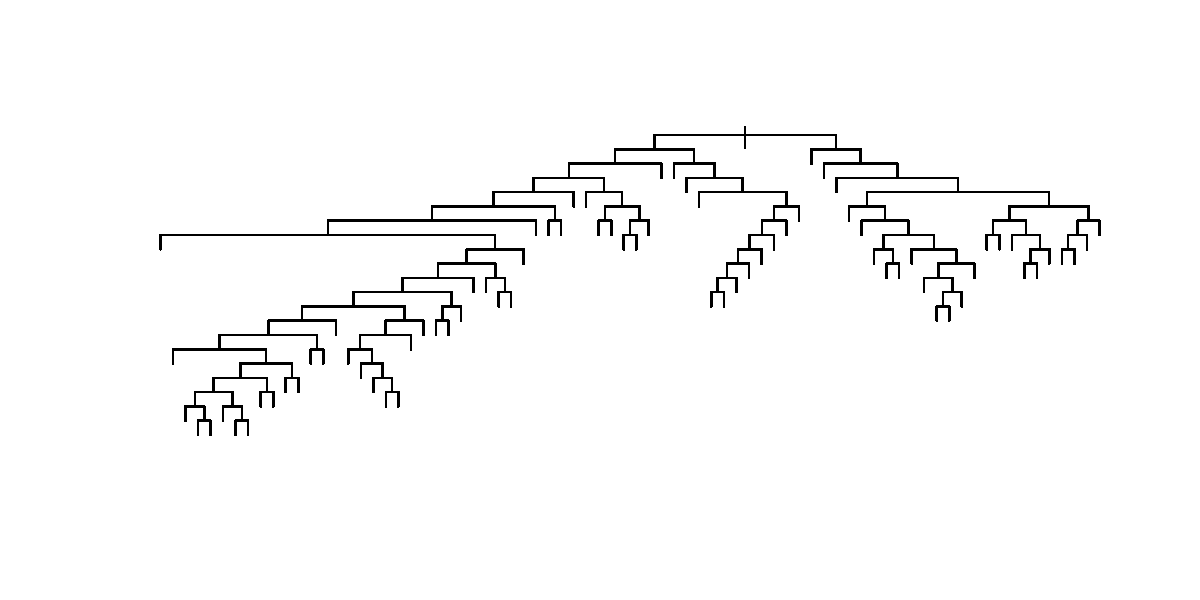
\epsfig{file=Spam/rpartTree00001, angle =90}
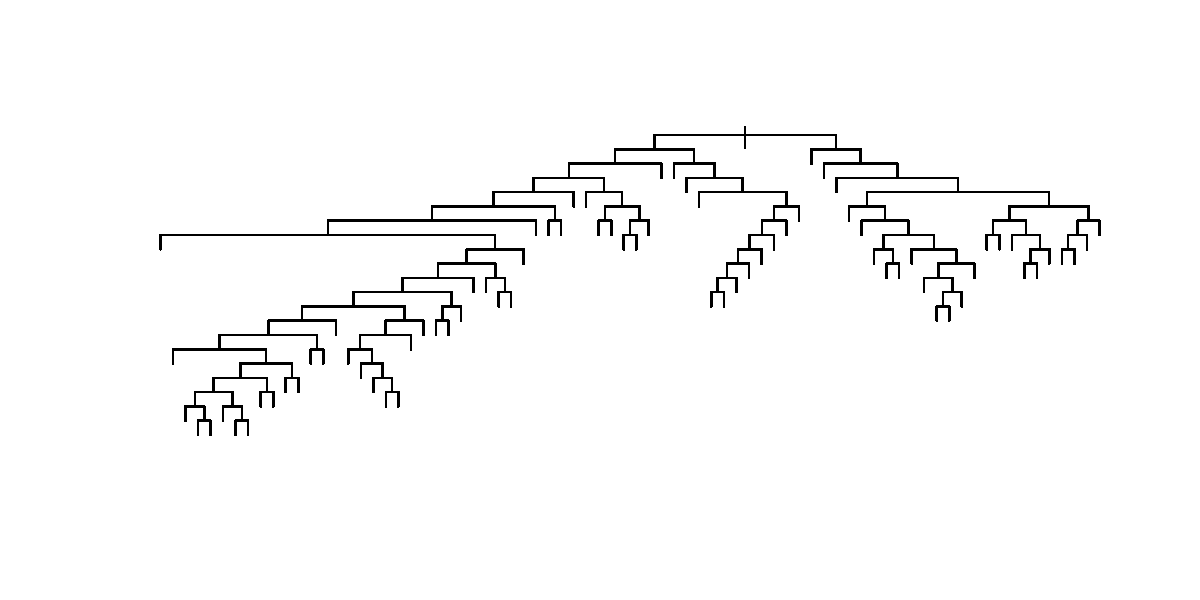
\includegraphics[angle=90]{Spam/rpartTree00001.pdf}
\caption{Classification tree for spam built using a complexity
paramater value of 0.00001 in the call to \Sfunc{rpart}}
\label{fig:rpartTree00001}
\end{figure}
\end{comment}

\begin{verbatim}
load("knnData.rda")
library(rpart)

#Convert logicals to factors
factorVars = as.data.frame(
                  lapply(derivedEmails[,logVars],as.factor))
rpartVars = cbind(factorVars, derivedEmails[,conVars])

#Fit a classification tree to classify spam
rpartFit = rpart(isSpam ~ ., data = rpartVars, 
                 method = "class")

plot(rpartFit, uniform = TRUE)
text(rpartFit)

# Fit a classification tree with smaller complexity parameter
rpartFit0001 = rpart(isSpam ~ ., data = rpartVars, 
                method="class", 
                control = rpart.control(cp=0.0001) )

# Classify the original data using the tree
oPreds0001 = predict(rpartFit0001, 
                newdata = rpartVars[,names(rpartVars) != "isSpam"], 
		type="class")

# Compute the type I and II errors 
> 1 - sum(as.logical(oPreds0001) & derivedEmails[,1])
          /sum(derivedEmails[,1]) 
[1] 0.09830508
> sum(as.logical(oPreds0001) & (!derivedEmails[,1]))
         /sum(1-derivedEmails[,1]) 
[1] 0.02076044

# Try classification on the new email messages, using the 
# tree obtained from derivedEmails
newFactorVars = as.data.frame(lapply(newEmails[,logVars],
                                     as.factor))
newRpartVars = cbind(newFactorVars, newEmails[,contVars])

nPreds00001 = predict(rpartFit0001, 
               newdata =
                 newRpartVars[,names(newRpartVars) != "isSpam"], 
                              type="class")

# The Type I and II errors shoot up 
> 1 - sum(as.logical(nPreds0001) & newEmails[,1])
          /sum(newEmails[,1]) 
[1] 0.18
> sum(as.logical(nPreds0001) & (!newEmails[,1]))
          /sum(1-newEmails[,1])
[1] 0.086
\end{verbatim}

A small complexity parameter produces a tree with more branches
%(Figure~\ref{fig:rpartTree00001}), 
and we can reduce the Type I and
II errors to 2\% and 10\% respectively. 
Table  shows the Type I and II errors for various values
of the complexity parameter.
Both errors reduce as the complexity parameter shrinks,
but when applied to the new email messages both
types of errors are much larger.
In comparison to $k^{th}$ nearest neighbor,
the best fitted tree when applied to
the new email messages does no better 
in terms of Type II error, but is 
a big improvement for Type I error.

\begin{table}
\begin{tabular}{rrrrr}
       &  \multicolumn{2}{c}{Old Mail} & \multicolumn{2}{c}{New Mail} \\
Complexity Parameter       & Type I & Type II & Type I  & Type II  \\
0.01 & 0.151 & 0.177 & 0.196 & 0.340 \\
0.005 & 0.037 & 0.190  & 0.154  & 0.208 \\
0.001 & 0.027 & 0.086  & 0.102 & 0.132 \\
0.0001 & 0.021 & 0.098 & 0.086  & 0.18 \\
0.00001 & 0.021 & 0.098 & 0.086  & 0.18 \\
\end{tabular}
\end{table}
 
%\chapter{Election Maps}

\section{Introduction}\
The ability to display geographically oriented data on maps is an 
indispensable tool for statisticians.
Election results are one example of such data, for votes are tallied according 
to political boundaries.
Well known to all of us is the map (Figure~\ref{fig:statemapredbluelarge})
that displays the results of the 2004 US presidential election
where each state is colored red for Republican or blue for Democrat according 
to whether Bush or Kerry received the most votes in the state. 
We explore alternative ways for displaying these 
election results that attempt to overcome some of the most
obvious drawbacks of this map--

\begin{figure}
\includegraphics{electionMaps/statemapredbluelarge.pdf}
%\epsfig{file=statemapredbluelarge}
\caption{ }
\label{fig:statemapredbluelarge}
\end{figure} 

\begin{itemize}
\item The map in Figure~\ref{fig:statemapredbluelarge} gives the false impression
that about 3/4 of the country voted Republican because
land area does not accurately represent population.
The red states cover far more geographic area than the blue ones, but
they have smaller populations than the blue states; in other words,
the blue states are small in area but large in terms of voters.
Across the United States, Bush received approximately 62 million votes (51\%) 
in the election,
Kerry received about 59 million (48\%) and Nader 400,000 (1\%), a far cry from 
the red-blue land area comparison. 

\item Further, in many states the election was quite close.
In Iowa Bush received 50\% of the vote compared to 49\% for 
Kerry; in Ohio the split was 51\% (Bush) to 49\%; and in Pennsylvania
it was 51\% Kerry for to  49\% for Bush. 
Where a state lands on the continuum from 0 to 100\% voting Republican 
is not apparent in the map.
The vote in Ohio's closely contested race looks no different than
the vote in North Dakota, where Bush's support was 63\%.
In terms of electoral college votes these distinctions make little
difference because the candidate who wins the popular vote takes all of
the electoral college votes for that state, but the additional information 
is helpful for a more in-depth assessment of the popular vote. 
\end{itemize}

In this chapter we will make election maps that attempt to address these
and other issues. Our first step is to recreate the 
map in Figure~\ref{fig:statemapredbluelarge}.
To do this we need to 
\begin{itemize}
\item acquire the data (vote counts for each state)
\item find and learn how to use map-making software 
\item analyze and map the data
\end{itemize}
Once acquainted with the data and software at hand,
our next step includes a more in-depth analysis that considers
the two issues raised about geographic area and color.
Then in a third round of map making, we go further in our analysis to address
other issues such as the granularity of the information presented 
and whether additional information that is geographically oriented may 
bring more insight to and further enrich our map.
In all of these phases, the three tasks of data acquisition,
learning about software, and data analysis, and the interplay
between these three tasks, are very important  in the process
of creating our map.
For example, data analysis may lead to new ideas for mapping
the data which require us to learn more about how the software
works, or it may lead to ideas about other data to collect
and include in the map.  Reciprocally, the task of
finding and cleaning data may give us ideas about how to analyze and
map it, or exploring the software may provide alternative ideas for
presentation and data organization.
This chapter highlights this process as we twice revisit our 
main goal of producing an election map, each time delving more
deeply into these three tasks as our maps change and evolve.


\section{Get out the votes}

Our first task in making a map like the one shown in 
Figure~\ref{fig:statemapredbluelarge}
is to get the official vote tallies for each state.
A search on \URL{www.google.com} with the keywords
``2004 official presidential election results" points us to
a Wikipedia site that has ``certified results" by state.
A little more snooping brings us 
to the Federal Election Commission website
and the official voting tallies for
each state can be found in a six-page pdf file 
at \URL{www.fec.gov/pubrec/fe2004/2004presgenresults.pdf}
(Figure~\ref{fig:officialElRes} contains a few snippets of it).
We see that over a dozen candidates ran for president from
parties that include the American Independent, Green,
Independent, Libertarian, and Peace and Freedom.

\begin{figure}
\includegraphics[height=2in,width=6in]{electionMaps/officialElRes1.pdf}
\includegraphics[height=2in,width=6in]{electionMaps/officialElRes2.pdf}
\includegraphics[height=2in,width=6in]{electionMaps/officialElRes3.pdf}
%\epsfig{file=officialElRes1,height=2in,width=6in}
%\epsfig{file=officialElRes2,height=1.5in,width=6in}
%\epsfig{file=officialElRes3,height=1.5in,width=6in}
\caption{ }
\label{fig:officialElRes}
\end{figure}
 
Other sites that appear high in Google's ranking include those
of news agencies, such as CNN, CBS, and USA Today.
The USA Today site 
\begin{verbatim}
http://www.usatoday.com/news/politicselections/vote2004/
  nationalelectionresultsbystate.aspx?oi=P&rti=G&cn=1&tf=l
\end{verbatim}
lists elections results from all
states on a single web page with each state in a separate table.
Whereas the CNN site presents each state separately, accessible
via a pull-down menu from\\
\URL{http://www.cnn.com/ELECTION/2004/pages/results/president/}.\\ 
On closer inspection of the voting results, we see that the CNN vote
counts exactly match those presented on the FEC site,
but the USA Today counts do not exactly. 
These discrepancies may be explained by the publication
dates of the data: the date on the document with the official government 
numbers is Feb 24, 2005, and those reported by USA Today have a date of 
Nov 11, 2004.  

Several options present themselves: although it is a bit more complicated to extract data
from a pdf formatted file, we could do this; we could also let Google
do the extraction for us (Google routinely provides HTML versions of
pdf files) and then extract the figures from the HTML;
we could pull the official numbers from the CNN site,
or the unofficial numbers from the USA Today site.
For the first map, we extract the data from the CNN site, and in a later
section we will use the USA today site because it offers an example of how to 
extract data remotely within R from web forms.

Refer to XML chapter for how to go about extracting the data.

Should  we add a function that creates a list(?) or
a  data-frame (?) or a CSV file from a html table?

PUT CODE HERE


\subsection{Map Software}
Our next task is to find software for making geographic maps.
Back on \URL{google.com} the search for 
``map software geographic open source" turns up many
sites related to open source Geographic Informations Systems.
GRASS GIS (Geographic Resources Analysis Support System) at 
\URL{grass.itc.it} looks promising.
The site \URL{opensourceGIS.org} provides scores of links to 
open source GIS-related software.
One that catches our eye is \URL{www.gstat.org}
which is described there as a computer program for geo-statistical
modeling, prediction, and simulation.
It is available as an R package and can read GRASS databases.
On closer inspection of the package on the Comprehensive R Archive
Network (CRAN) site at \URL{cran.us.r-project.org}, 
we find that the emphasis of the package is on
statistical modeling (kriging and variograms) not on mapping.
We also notice a GRASS R package that allows one to call R from
within GRASS.
Rather than pursue these angles, we look for other R packages 
that can make maps because our focus here is
on demonstrating how to find and learn about software not
on learning GIS systems (although that is a useful tool for
statisticians to have). A Google search for ``R geographic map"
turns up two packages, \RPackage{Rmap} and \RPackage{maps},
the later is on CRAN. A third search on Google, this time
for  ``R cran map" turns up a site 
\URL{http://sal.agecon.uiuc.edu/csiss/Rgeo/maps.html}
that describes the map-related R packages both on CRAN and not.  
These include,

\noindent 
\RPackage{mapdata} - Extra Map Databases;\\
\RPackage{mapproj} - Map Projections;\\
\RPackage{maps} - Draw Geographical Maps;\\
\RPackage{maptools} and \RPackage{shapelib} - Tools for reading and handling shape files;\\
\RPackage{rgdal} - provides bindings between R and GDAL for accessing
image and raster data.\\
\RPackage{RArcInfo} - provides an interface to read geographic information in
Arc/Info format.\\


It appears that \RPackage{maps} might work for us.
Packages on CRAN each have a web page where we can download the zipped package
source, view the index of the package contents, and read the reference
manual.
The documentation for the \RPackage{maps} package lists the functions in alpha order,
which is not all that helpful when trying to figure out how to start
to use a package.  We would prefer the central most important functions 
to be listed first in a general overview of the package with examples.
A search online does not uncover any vignettes or  tutorials on how to use the
\RPackage{maps} package, and skimming the contributed documentation on CRAN
we do not find any examples of maps.

Let's install the package and proceed from there  with our exploration of the
package's user philosophy.
To do this, we download and save the package source 
\verb+maps_2.0-27.tar.gz+.
The name of the package includes the version, 2.0-27.
[What does that mean?]...
Also we see on the web page that the package depends on
R version 1.7.0 or higher, since we are running version 2.0.1 
we should have no problems.
If we do have trouble, the maintainer of the package is
listed, and the reference manual contains his contact information.
Also, we can post questions to the R help mailing list 
at \URL{http://www.r-project.org/mail} or
check on the help mailing-list archive to see if our question has 
been answered already. 
(Currently there are about 500 messages referring to the 
\RPackage{maps} package on the archive).
Finally, this page also tell us that the software has a GPL2 license
[WHAT does that mean]...

Once we download the package, to install it we simply run 
R with additional run time arguments:
\begin{verbatim}
R CMD INSTALL maps_2.0-27.tar.gz
\end{verbatim}
[WHAT about environment variables....]
[ What about Mac vs windows vo linux]

Now to continue our research on how the package works, we look for a demo.
The command
\begin{verbatim} 
> demo(package = .packages(all.available = TRUE))
\end{verbatim}
indicates there are no demos for \RPackage{maps}.
Next, we turn to the R help facilities, we start the R help in our browser,
\begin{verbatim}
> help.start()
\end{verbatim}
and look up the \RPackage{maps} package. 
There we find a list of the functions that are documented. 
These  form a subset of the functions that are part of the package. 
The others are not documented because they are generally for internal
use by the package, not the user. 
To see the complete list of functions, 
we call \SFunction{objects} with the argument $3$, 
\begin{verbatim}
> objects(3)
 [1] "apply.polygon"        "area.map"             "area.polygon"        
 [4] "as.matrix.polygon"    "centroid.polygon"     "char.to.ascii"       
 [7] "closed.polygon"       "gp.smooth"            "identify.map"        
[10] "in.one.polygon"       "in.polygon"           "indicators.factor"   
[13] "insert"               "is.regexp"            "kernel.region.region"
[16] "kernel.region.x"      "kernel.smooth"        "makepoly"            
[19] "map"                  "map.axes"             "map.cities"          
[22] "map.old"              "map.poly"             "map.scale"           
[25] "map.text"             "map.where"            "map.wrap"            
[28] "mapgetg"              "mapgetl"              "mapname"             
[31] "mapthin"              "maptype"              "match.map"           
[34] "match.map.grep"       "match.map.slow"       "num.polygons"        
[37] "range.polygon"        "smooth.map"           "sub.polygon"         
[40] "subgroup"            
\end{verbatim}
The argument of $3$ tells R where in the search path for our session
to find \SPackage{maps},
\begin{verbatim}
> search()
 [1] ".GlobalEnv"        "package:mapproj"   "package:maps"     
 [4] "package:methods"   "package:stats"     "package:graphics" 
 [7] "package:grDevices" "package:utils"     "package:datasets" 
[10] "Autoloads"         "package:base"     
\end{verbatim}
We see that the package of interest is the third in line in the search path,

We have found that \SFunction{map} is the main entry
point in the package. To get a quick idea for the user-model for
the package, we run the examples provided by the documentation for
\SFunction{map},
\begin{verbatim}
> example(map)
\end{verbatim}
We discover that the simple command \verb+map("state")+ is a 
good starting point.
It provides a state map of the 48 contiguous states.
The example code for \SArg{state} fills the states with
colors.
\begin{verbatim}
map('state', fill = TRUE, col = palette() )
\end{verbatim}

Before making our election map, we need to understand better the map interface.
The documentation for the \Sfunction{map} function provides 
a simple form: 
\begin{verbatim}map(database, regions)
\end{verbatim} 
where the argument \SArg{database} is described as a
\begin{quote}
character string naming a geographical database, or a list of x, y, and names obtained
from a previous call to map. The string choices include a world map, three 
USA databases (usa, state, county), and more (see the package index). 
\end{quote}
The second argument, \SArg{regions} takes a character vector that names the polygons 
to draw. For example, the state of California is one such polygon in the 
state database.  According to the documentation, for those states 
composed of more than one polygon, 
the individual polygons have the name of the region, 
followed by a colon and a qualifier, as in michigan:north and michigan:south. 
The \SArg{exact} argument is boolean used to specify whether exact matching
(\STrue) or regular expressions are used in matching region names.

Given, the state map example in the documentation, it appears that the 
\SArg{fill} and \SArg{col} arguments are needed to color states red and blue. 
According to the documentation, the \SArg{col} argument takes a vector of colors. 
When the \SArg{Fill} argument is \STrue then 
``the colors are matched one-one with the polygons that get selected by the 
region argument (and are reused cyclically, if necessary)." 

To learn more about the databases that the function takes, we refer to
the documentation for \SVariable{state} describes it as a follows:
\begin{quote} 
The data file is merely an assignment to a character string which specifies 
the name of an environment variable which contains the base location of the 
binary files used by the map drawing functions. 
This environment variable (R\_MAP\_DATA\_DIR for the datasets in the maps package) 
is set at package load time if it does not already exist. 
\end{quote}

Overall, the documentation does not completely satisfy us and we turn to
the references listed there.
The paper, ``Maps in S", by the authors of the 
original code, Becker and Wilks, looks promising.
According to them,

\begin{quote}
The map function is an interface to geographical databases. 
%In developing its capabilities we have used data supplied by the US Census Bureau 
%(see References), which describes all county boundaries in the United States. 
%From this data we constructed three geographical data-bases with information
%on national, state and county boundaries in the USA. 
...
The information in each geographical database is organized into three files. 
The first file has descriptions of polylines. 
These are sequences of points on the earth's surface, which, when joined in order 
by line segments, form a part of the map, typically a political or natural boundary. 
The second file describes polygons in terms of polylines, 
that is, each polygon is given as a list of polyline numbers, 
indexing polylines from the polyline file, which, 
when traversed in the given order, form a closed area of the map. 
Finally, a third file gives names to each of the polygons in the second file. 
It is primarily through these names that the map data is accessed. 
Polygons are named with a convention that allows several polygons to be accessed with
one name, such as referring to the two parts of Michigan with the name ``Michigan.''
\end{quote}

To summarize the process just completed, to look for entry points
in unfamiliar software and to understand the philosophy behind
the use interface, we  

\begin{itemize}
\item search the web for vignettes and tutorials 
\item run demos and examples, such as with \SFunction{demo}
and \SFunction{example}
\item call up the help system, e.g. \SFunction{help.start}
\item read package documentation 
\item track down references in the documentation 
\item search the mailing list archive
\item look for other, undocumented entry points, e.g. \SFunction{objects}
\end{itemize}

Armed with this information about \RPackage{maps}, 
we turn our attention to reproducing the map in 
Figure~\ref{fig:statemapredbluelarge}.

\subsection{Analysis and map making}
The analysis of our data is straightforward in this phase:
we compare vote counts to determine the winner in each state.
For these purposes we can simply compare votes for Bush to votes for
Kerry and ignore the results from the other candidates.
The object \SVariable{stateColor} is a character vector of length 49
for the 48 contiguous states plus the District of Columbiacolumvbia.
The values are ``red" or ``blue" according to whether Bush or 
Kerry won the popular vote in the state. The names of the 
elements are the corresponding state names. 
\begin{verbatim}
> map("state", names(stateColor), col = stateColor, fill = TRUE)
\end{verbatim}
The resulting map is in Figure~\ref{fig:statemapwrong}. 
Something went wrong; New Jersey, New York, Pennsylvania, and 
Washington are red instead of blue.

\begin{figure}
\includegraphics[height=3in]{electionMaps/statemapwrong.pdf}
%\epsfig{file=statemapwrong,height=3in}
\caption{Notice that Pennsylvania, New Jersey, New York, and Washington are red.}
\label{fig:statemapwrong}
\end{figure} 

To trouble shoot the problem we:

\begin{itemize}
\item Check our input vector for correct matching of
state name and color: There does not appear to be a problem
with our input.

\item Try a few simple cases to see if we get what we expect:  
A plot of the region consisting of
Minnesota, Michigan and Texas with the colors red, blue and green,
in that order, yields a surprising result (see Figure~\ref{fig:michigantexas}).
Given our understanding so far, we expect Minnesota to be red, Michigan blue, 
and Texas green. Instead we see that Minnesota is green and Michigan has 
two colors. 
 
\begin{verbatim}
> map("state")
> map("state", c("minnesota","michigan","texas"),
      col = c("red","blue","green"), fill = TRUE, add = TRUE)
\end{verbatim}

\begin{figure}
\includegraphics[height=3in]{electionMaps/michigantexas.pdf}
%\epsfig{file=michigantexas,height=3in}
\caption{A call to the map function with the region Minnesota, Michigan and Texas
and the colors red, blue and green, produced a plot with Minnesota green not red,
Texas red not green, and Michigan two colors.}
\label{fig:michigantexas}
\end{figure} 

\item Save and examine the results from a call to the function:
\small{
\begin{verbatim}
> mapResult = map("state", plot = FALSE)
> class(mapResult)
[1] "map"
> names(mapResult)
[1] "x"     "y"     "range" "names"
> length(mapResult[[ "names" ]])
[1] 63
> mapResult[[ "names" ]][ 53:63 ]
 [1] "virginia:chesapeake"        "virginia:chincoteague"     
 [3] "virginia:main"              "washington:san juan island"
 [5] "washington:lopez island"    "washington:orcas island"   
 [7] "washington:whidbey island"  "washington:main"           
 [9] "west virginia"              "wisconsin"                 
[11] "wyoming"                   
\end{verbatim}
}
The output from a call to \SFunction{map} is an object of 
class map with four elements, \SVariable{x}, \SVariable{y},
\SVariable{range}, and \SVariable{names}.
There appear to be 63 named regions, each corresponding to a polygon,
and named according to the convention described in the previous section.
The name matching apparently does not work the way we expected.

\item Return to the documentation and read it more carefully: 
In the documentation for \SFunction{map} and \SVariable{state}
we do not see a mention of this issue, but we discover the 
function \SFunction{match.map}, which assigns an index to 
each map region and is ``useful for map coloring."

\small{
\begin{verbatim}
> colorIndex = match.map("state", names(stateColor))
> colorIndex
 [1]  1  2  3  4  5  6  7  8  9 10 11 12 13 14 15 16 17 18 19 20 20 20 21 21 22
[26] 23 24 25 26 27 28 29 30 31 31 31 31 32 32 32 33 34 35 36 37 38 39 40 41 42
[51] 43 44 45 45 45 46 46 46 46 46 47 48 49
\end{verbatim}
}
\end{itemize}

The example in match.map shows how to solve the problem.
\begin{verbatim}
map("state", names(stateColor), col = stateColor[colorIndex], fill = TRUE)
\end{verbatim}
We now have a map that is in agreement with Figure~\ref{fig:statemapredbluelarge}.


\section{One acre one vote}
In our example, the geographically oriented data the unit of interest is
typical population, not 
Election results pertain to people. 
Geographic information, where the people live 
Maps of election results aim to show who voted for Bush or Kerry and where they live. 
A difficulty that arises with adding population information to geographic maps pertains
to the uneven population density in the region. 
The colored maps shown here fill the state region with a color to indicate 
how the people of the voted, 
but the states with lower population densities are over-represented in these maps.

Cartograms reshape the map while maintaining geographic boundaries, 
so the area of the regions are proportional to the variable of interest, 
which is population in our case. 
Statisticians, cartographers, and physicists have considered the problem of 
constructing cartograms for the 2004 presidential election results. 
See for example, the cartograms of Venkatasubramanian (Figure~\ref{})
and Gastner, Shalizi, and Newman (Figure~\ref{}).
The later group uses the linear diffusion process of elementary physics to 
create a map where the geographic boundaries are distorted to represent population. 
That is, given a particular population density, they allow the population to 
flow away from high-density areas, stretching the boundaries of regions, in order
to equalized the density everywhere.


\begin{figure}
\includegraphics[height=3in]{electionMaps/venkatasubramanian.pdf}
\includegraphics[height=3in]{electionMaps/gastnerNewman.pdf}
%\epsfig{file=venkatasubramanian,height=3in}
%\epsfig{file=gastnerNewman,height=3in}
\caption{}
\caption{}
\label{fig:cartograms}
\end{figure}

\begin{figure}
\includegraphics{electionMaps/stateCirclesRB.pdf}
%\epsfig{file=stateCirclesRB}
\caption{}
\label{fig:stateCirclesRB}
\end{figure}

For a more simplistic approach that does not distort the geographic region,
but uses color in areas that are proportional to population, we superimpose symbols
of different sizes on the map at appropriate locations.
Figure~\ref{fig:stateCirclesRB} is an example. 
The area of the circles is proportional to the voters in the state, 
and the center of each circle is placed at the center of the corresponding state.
To add the circles to the states, we must find the state centers.
The \SPackage{maps} package documentation lists several 
internal functions related to polygons, which we can also see
with a call to \SFunction{objects}.
\begin{verbatim}
area.polygon(p) 
centroid.polygon(p) 
as.matrix.polygon(x) 
closed.polygon(p) 
in.one.polygon(p, x)
in.polygon(p, x) 
num.polygons(p)
range.polygon(..., na.rm = FALSE) 
sub.polygon(p, i) 
\end{verbatim}

These functions are not exported to the user.
That is, a call to help does not reveal any documentation on how to use 
these functions because it is expected that we will not need them.
However, the source code for \SFunction{centroid.polygon}
is well enough documented for us to figure  out that if we call 
it passing the \SArg{x},\SArg{y} coordinates of the 
polylines of the polygon of interest, then it returns the centroid
of that polygon.
To get the polylines, we store the results from a call to 
\SFunction{map} to plot the \SArg{state} database, which we know 
has vectors \SArg{x},\SArg{y} corresponding to the polylines
for the state polygons with the coordinates for each polygon
marked by \SNA.  We write the function \SFuntion{polys} to 
split up these vectors into a list of vectors, one for each
polygon. Then all we need to do is apply the \SFunction{centroid.polygon} 
function to each element of our list. Finally, we discard the extra polygons for 
those states made up of more than one polygon. 
\begin{verbatim}
mapR = map("state", plot=FALSE, fill= TRUE)
statePolys = polys(mapR[["x"]],mapR[["y"]])
stateCenters = sapply(statePolys, centroid.polygon)

#pick out index for one polygon from each state
onePoly = sort( c( (1:63)[- grep(":",mapR[["names"]])],
                          grep(":south",mapR[["names"]]),
                          grep(":main",mapR[["names"]]) ) )
stateCenters1 = stateCenters[ onePoly,]
\end{verbatim}

How do we decide on the size of the circles? 
We make the area proportional to the number of voters, 
which implies the radius is proportional to the square root of voters.
We further scale the total number of voters in the state by the 
maximum over all states so it fits the scale of the map.
\begin{verbatim}
# determine the radius of each circle
totalVote = bushVote + kerryVote
maxV = max(totalVote)
stateRad = 3*sqrt(totalVotes/maxV)

# determine the color of each circle
colorsRB = ifelse(bushVote > kerryVote, 
               rgb(1, 0, 0, 0.5), rgb(0, 0, 1, 0.5))

map("state")
symbols(stateCenters1[1,], stateCenters1[2,], circles = stateRad,
         add = TRUE, inches = FALSE, fg = colorsRB, bg = colorsRB)
\end{verbatim}

The circles give a much more accurate representation of the support
for Bush versus Kerry. They have been colored using transparency, which
allows us to see the overlapping states in the densely populated
northeastern part of the country.


\section{Winner take all}
Continuous data are often collapsed or transformed into categories or factors. We do this for many reasons: convention dictates it, data reduction makes the task manageable, or the categories are relevant to the analysis. But data reduction can yield a misleading or less-informative analysis. Take for example the map shown below, which appears on the USA Today website . Here, the percentage of votes for Bush in a county in the 2004 presidential election are converted to the categorical information as to whether Bush won or lost the vote in the county. A county is colored red for a Bush win and blue for a Bush loss (Kerry win). What information loss is there?

\begin{figure}
\includegraphics{electionMaps/stateTherms.pdf}
%\epsfig{file=stateTherms}
\caption{}
\label{fig:stateTherms}
\end{figure}

\begin{figure}
\includegraphics[height=3in]{electionMaps/bushPropHist.pdf}
%\epsfig{file=bushPropHist,height=3in}
\caption{}
\label{fig:statePropHist}
\end{figure}

\begin{figure}
\includegraphics{electionaps/stateSquareBrewerLegend.pdf}
%\epsfig{file=stateSquareBrewerLegend}
\caption{}
\label{fig:stateSquareBrewerLegend}
\end{figure}

\begin{figure}
\includegraphics{electionMaps/stateBrewerTrans.pdf}
%\epsfig{file=stateBrewerTrans}
\caption{}
\label{fig:stateBrewerTrans}
\end{figure}


However, with these two maps we can't tell if Bush won by a landslide, if the election was close, or if he lost by a landslide in the counties and states (respectively). That is, we have lost the information as to how close the election was in the county or state. Robert Vanderbei at Princeton University suggests using shades of purple to indicate the percentages of votes cast for Bush versus Kerry. His map appears below,

We get a much different impression of the voting patterns of Americans from this map. However, one drawback with the use of purple that has been pointed out at  http://homepage.mac.com/tcp/PurpleAmerica/

    Red shades tend to stand out more to the human eye than blue shades of the same saturation. As such a blended or ``purple" map of the US, based on the popular vote will tend to look a little more red than blue in its hue, given the bias of the human eye. 

See Brewer notes - we can get help outside of R

Purple maps in the press - problem is that they look red to the eye

Schema for color - depends on whether the data trying
to portray are sequential, diverging, or qualitative
Explain each of these and give some examples

How to specify colors in R that are more than Red and blue?
RGB is one way.

brewer.pal

How many variations in color do we use?
How do we determine the intervals? We can use percentiles,
percentages, square root, log....

Now the circle can be reduced to one 


\section{Granularity}
Level of the data - we can't know how an individual
votes, only the tally of results from a polling place,
or precinct.

County level data

Granularity of data --

For precinct level results we  
need to visit the individual State Records offices,
overseen by the Secretary of State.
The urls for these can be found at the 

\URL{http://www.fec.gov/pubrec/staterec.htm}

States are not obligated to store their data in same format.
Take Alabama and Wyoming for example. 

Alabama
Office of the secretary of State for the State of Alabama.

\URL{http://www.sos.state.al.us/election/2004/index.cfm}


to obtain an Excel files

Wyoming on the other had offers pdf files, one per precinct,
available at 

http://soswy.state.wy.us/election/2004/results/04-g-pp.htm

Precinct level is hard to come by. 
State level is easier. We can extract the official results from
the pdf file (HOW)
or use the election results posted on the web by the 
news agencies, such as USA Today and CNN. 
\begin{verbatim}
http://www.usatoday.com/news/politicselections/vote2004/
      nationalelectionresultsbystate.aspx?oi=P&rti=G&cn=1&tf=l
\end{verbatim}

% Change the sp=
%http://www.usatoday.com/news/politicselections/vote2004/PresidentialByCounty.aspx?oi=P&rti=G&sp=NJ&tf=l

This is how we can use XPath to get the data.

By looking at the HTML for NJ  (and MA), we can see that the 
first row of the table of interest start with 
\begin{verbatim}
<td class="notch_white" width="153"><b>Atlantic</b></td>
\end{verbatim}
It is the notch_white that identifies this table.
One has to make certain of this.
But if we could find that node and then go up
the tree from that to find its parent -- the row (tr) --
and then its parent -- the table, 
we could sweep over all the children and extract the
data.
So, if we use the following code
\begin{verbatim}
z = htmlTreeParse("http://www.usatoday.com/news/politicselections/vote2004/PresidentialByCounty.aspx?oi=P&rti=G&sp=NJ&tf=l", useInternal = TRUE)
v = getNodeSet(z, "//td[@class='notch_white']")
tb =xmlParent(xmlParent(v[[1]]))
\end{verbatim}
Alternatively, we could find all td elements with
a class of notch_white or notch_light and a width.
\begin{verbatim}
v = getNodeSet(z, "//td[@width and @class='notch_light' or @class='notch_white']")
\end{verbatim}
(We need the width or we would pick up the note at the bottom of
the table of ``Vote returns will appear shortly...''.
But we could identify this as not having multiple td elements.)
This  gives all the cells of the table, not just the first element
of each row.  It also gives back the one without the width.
We can identify this as the ``last'' one or alternatively as the one
with more than one child
\begin{verbatim}
table(sapply(v, xmlSize))
v = v[sapply(v, xmlSize) == 1]
\end{verbatim}
Then, we can fetch the values for each cell with
\begin{verbatim}
vals = matrix(sapply(v, xmlValue), , 6, byrow = TRUE)
vals = as.data.frame(vals)
vals[-1] = sapply(vals[-1], function(x) as.integer(gsub(",", "", as.character(x))))
\end{verbatim}
Note that we have to handle the commas in the numbers
and it is easy to just remove them.

So we can put all of this in a function
\begin{verbatim}
getStateVotes =
function(state) {
  uri =paste("http://www.usatoday.com/news/politicselections/vote2004/PresidentialByCounty.aspx?oi=P&rti=G&sp=",state, "&tf=l", sep = "")
  z = htmlTreeParse(uri, useInternal = TRUE)
  v = getNodeSet(z, "//td[@width and @class='notch_light' or @class='notch_white']")
  v = v[sapply(v, xmlSize) == 1]
  vals = matrix(sapply(v, xmlValue), , 6, byrow = TRUE)
  vals = as.data.frame(vals)
  vals[-1] = sapply(vals[-1], function(x) as.integer(gsub(",", "", as.character(x))))
  vals
}
\end{verbatim}

To get all the state abbreviations, we looked up ``state
abbreviations'' on the web and cut and pasted the results into
We should do this properly.
\begin{verbatim}
abbrevs = readLines("~/Classes/StatComputing/Book/electionMaps/stateAbbrevs")
abbrevs = abbrevs[nchar(abbrevs) == 2]
\end{verbatim}
This gives 59 values, yet we expected only 51 (including the
district of Columbia (DC)). We also get Western Samoa, etc.
So we either want to remove these or make the function
robust to handling errors in retrieving the URI.
And in fact it is.
\begin{verbatim}
stateVotes = lapply(abbrevs, getStateVotes)
names(stateVotes) = abbrevs
\end{verbatim}


Where do we get county centers?  -- learn more about the software

Why doesn't our circle show up?
do we need mapproject?

Use the locator function to see what's going on.
Place axes on the map so that we can see if we have the right units
We find that X and Y are reversed
We also find that X and Y are on the wrong scale

problem with jitter

problem with cex

\subsection{reconciling the differences between various sources}

Missing counties

Counties with different names

Parish, Bourough, Townships and Counties


\section{Additional data}

\subsection{Census data}
How to get it

Antoehr data source to reconcile

How to portray it

\subsection{Adding Markers to the Map}    

cities\\
titles\\
legends\\
map markers do not all work the same way as the plot function



=========================================

[A CHAPTER on GIS?  -- or include it as an example of Intersystem interfaces? ]

%Notice that the data are a bit more complicated because there are
%more candidates running than Bush and Kerry
%In Alaska Nader, Peroutka (American Independent), Badnarik (Libertarian), 
%and Cobb (Green)
%In Arizona only Bush, Kerry and Badnarik
%In California Badnarik, Cobb, Peltier (Peace and Freedom), and Peroutka 

%We examine a few other packages, and read the 
%accompanying documentation.

%Although we are not interested in the map of china and new zealand
%found in mapdata package we may be interested in the map,world

%mapproj converts latitude and longitude into projected coordinates.
%map.grid draws a grind on an existing map
%maproject converts latitude and longitude into projected coordinateso

 
%\input{Geolocation/Geolocation}


\chapter{Advanced Graphics}

\begin{summary}
  In this chapter, we focus on more advanced aspects of graphics
  within R and also look at creating graphics that can be displaed in
  other aplications such as Google Earth and also deployed on the Web
  and provide animation and interactivity.  The purpose is to show the
  reader how to create their own complex plots and also to illustrate
  that visualization is a vital field that is much broader and more
  modern than traditional statistical graphics.
\end{summary}

\section{Grid Graphics}

\section{Display Geographic Data with Google Earth: KML}

\section{Graphics on the Web}

\subsection{Scalable Vector Graphics}

\subsection{Flash}

\subsection{JavaScript}

\chapter{Programming with Extensibility in Mind}

\textsl{
The content in this chapter could be merged into 
the second chapter on programming and the
chapter on writing software and R packages.
However, it may make sense to keep it separate and not 
confound it with other topics. The ``writing software''
chapter is already overladen with topics.
}

\begin{summary}
  This chapter is about the philosophy of, and practical approaches
  to, writing code that is extensible and reusable.  We outline why
  reusability is good, including avoiding re-testing when we make
  changes and of course the ability to avoid writing new similar code.
  We contrast the trade-offs of over-generalizing and not recognizing 
  generalities.  We try to characterize when such generalities might
  be present and how to recognize them.
  

  The chapter discusses how we write R functions using default values
  so that they allow callers to customize their behavior without
  having to specify the values.  We move on to object oriented
  programming, both S3 and S4 classes and compare these with
  C++/Java-style OOP.  We try to provide some real-life case studies 
  describing how we design classes and make decisions about the class
  hierarchy and method definitions.

  The purpose of this chapter is to encourage the reader to recognize
  that designing with flexiblity and extensibility in mind is
  empirically a good thing as we tend to reuse software.
\end{summary}

\section{The Purpose of Extensible, Reusable Code}

\section{Extensibilty via Default Arguments}

\section{Object Oriented Programming}

\section{S3 Classes \& Methods}

\section{S4 Classes \& Methods}

\section{Integrating S3 \& S4}

\section{C++/Java-style classes \& methods}



\chapter{Writing Software: Turning Code into Software}

In this chapter, we explore the transition from writing individual
commands, scripts and functions for your own use to writing software
that you can use in different projects or that others can use.

This chapter introduces numerous ideas and software.  It is intended
primarily for graduate students, at the PhD or Master's level.


Put error handling and exceptions/conditions somewhere in the book.

\section{Writing R packages} 

\subsection{Name spaces}

\subsection{Writing Documentation}

\subsection{Vignettes}
\textit{We might want to include this as a separate chapter
on dynamic documents.}

\section{Creating Tests for Functions}

\section{Change Logs}

\section{Todo Lists}

\section{Bug Tracking}

\section{Version Control}

\section{Portability, Installation and Configuration}

\section{Literate Programming}

\section{Etiquette and Behavior in Software Development and Open Source} 

\chapter{Efficient Code: Making code work faster}
\begin{summary}
In this chapter, we discuss how we go about improving code so that it
runs faster and/or uses less memory.  We present the basic ideas of
efficient code that are common to all languages, and also focus on
R-specific aspects.  We also cover the tools in R for measuring
performance. We go through the details of several real examples/case
studies and illustrate the way we think about writing code.  As with
the rest of the book, the goal here is not just to present the tools,
but to try to explain the way users should think about them and
comparing them to alternative approaches.
\end{summary}

\section{The basics of measuring code}
\Rfunc{system.time}

\subsection{Algorithmic Complexity: Theoretical and Empirical}
The idea that there is a relationship between size of input and the
number of computations and the time and memory the computations take. 
We won't spend very much time talking about the theoretical/algebraic
calculations one can perform for algorithmic analysis.
Instead, we focus  on practical ways to empirically estimate 
performance along with some of the difficulties or issues to 
consider (e.g. garbage collection, other tasks running on the machine,
comparing different hardware).


\section{Basic Guidelines for Efficient Code}

\begin{itemize}
\item  Vectorize calculations
\item  Pre-allocating the answer
\end{itemize}

\section{Profiling Code to find Bottlenecks}

\section{Profiling in Action}
Come up with an example similar in spirit to Ross'
excellent 5 step Random Walk example.

\section{Using C}
Here we talk at a high-level of using C code to make computations
faster. We don't show the C code, but more claim that we have it and
show the performance gains. We discuss a little bit about how the come
about because of compiled languages and the difference between
resolving symbols and the need for unboxing in interpreted languages.

\section{Introduction to High-level Distributed  Computing}
\subsection{The basic computational model}
Client-server, master-workers.
Breaking tasks 

\subsection{SNOW}

\subsection{Different Communication Approaches}
MPI/PVM

\subsection{Managing Data}
Here we talk about avoiding the transmission of data
and maximizing the number of computations per
byte transferred.

\chapter{Integrating Other Languages: C, Python, Perl, ...}

\begin{summary}
The primary focus in this chapter is on using C code within R (or
MATLAB, potentially also).  We start by discussing why we might want
to use existing C code within R.  We describe the different steps and
components in compiling, linking and loading compiled code into R,
contrasting this with the interpreted model that R and many other languages
use. We also present some of the tools that we can use to explore and
perform diagnostics on compiled code, e.g. ldd, otool and depends.exe
(on Windows) for examining dependencies on other DLLs,
nm for looking at symbols.

We look at both the \Rfunc{.C} and \Rfunc{.Call} interfaces.
We illustrate the standard marshalling techniques for .C().

We also discuss debugging using a debugger such as gdb
and work through a case study of finding a bug in C code.
We contrast this with using print statements.


We also talk about interfaces with other
systems and languages such as 
\begin{itemize}
\item the Unix Shell (via the \Rfunc{system} function which we have discussed in chapter~\ref{chap:Shells}),
\item Python (\Rpkg{RSPython} and \Rpkg{RPy})
\item Perl (\Rpkg{RSPerl}), 
\item MATLAB (\Rpkg{R.matlab} and \Rpkg{RMatlab})
\item Java (\Rpkg{rJava} and \Rpkg{RSJava})
\item DCOM  (\Rpkg{RDCOMClient} \& friends and \Rpkg{rcom})
\end{itemize}
We illustrate these by example. We won't go into all the details of
all the languages, but discuss the steps of 
\begin{itemize}
\item initializing the Virtual Machine
\item calling a foreign function from R
\item marshalling data between the systems
\item dealing with different computational models, e.g. R's generic
  functions and methods  and Python's objects and methods
\end{itemize}
We also show that most of these are actually simpler in many ways than
working with C/C++ code because of run-time reflection.
We'll also illustrate how we can use this to have code that writes
code -- \textit{meta-programming}.

We'll connect these inter-system intefaces back to Web Services via
SOAP, REST, XML-RPC.
\end{summary}

\section{Why use Compiled Code in R?}
The primary motivations are 
\begin{itemize}
\item  reusing existing code to avoid having to reimplement it
ourselves
\item speed/efficiency
\item writing code in a common language so that it can be used 
\end{itemize}

\section{An overview of Compiled Code: C/C++}
This covers the difference between
compiling, linking and loading DLLS.
Within compiling, we discuss the preprocessor and the compiler proper.
We also talk about different arguments that control the compilation
such as -I, -O2 and -g.
It talks about make files and dependencies.
It talks about linking to other libraries and the use of \verb+(DY)LD_LIBRARY_PATH+.

\section{The Basics of calling C from R : .C()}


\section{The Standard Marshalling of Data}


\section{Debugging Compiled Code}

\section{Automating the interface to routines and data structures}
Here we talk about SWIG and RGCCTranslationUnit.

\section{Writing C code ourselves}
Here we cover the basics of the C language so that 
readers can 

\section{The .Call interface}

We talk about the more advanced and flexible
way to call C code from R and how we can manipulate 
R objects.

We outline external pointers and how they can be used to handle
complex data that don't map to R objects and for dealing with large
data. We describe how this changes the semantics of R ``pass-by-copy''.



We'll also mention the \Rfunc{.External} function
and its \textit{raison d'etre}.

\section{General Interlanguage Interfaces: Combining systems and
  languages}
We talk about the general model.
Here we talk about calling Python or Perl from R.
For example, we can read the email data using Perl modules
and then deal with 


\section{Debugging C Code}
GDB

Break points
Conditional break points.

Attaching to existing/running processes.

Examing core dumps




\chapter{Bibliography}
%\bibliographystyle{plain}
%\bibliography{statcomp}

\end{document}
